\section{Introduction}
\title{Go by Example}
\author{@mmcgrana \and 訳:@oohira}

\maketitle

Go は、シンプルで高速な、信頼性の高いソフトウェアを開発するために設計された、オープンソースのプログラミング言語です。Goのコードやツールのパッケージ、モジュールについて学ぶには、公式ドキュメントを読んでください。

Go by Example は、コメント付きのサンプルプログラムを使った、ハンズオン形式のGoの入門編です。最初のサンプルに進むか、下のリストから読んでください。

この文書は、@mmcgranaさんにより作成されたGo by Exampleの日本語訳となります。



\section{Goの環境設定}
Goの世界へようこそ、さっそく初めてみましょう!

Goは新しい言語です、並列処理、ガベージコレクションを備え、軽快にコンパイルできる言語です。以下のような特徴を持っています:

\begin{itemize}
  \item 一台のコンピュータ上であっという間に大型のGoプログラムをコンパイルすることができます。
  \item Goはソフトウェアの構造にモデルを与えます。分析をより簡単にこなすことができ、ファイルやライブラリのincludeといったCスタイルの書き出しにありがちな部分を大幅に省くことができます。
  \item Goは静的型付け言語です。型に階層の概念が無いのでユーザはその関係に気をとられることもなく、典型的なオブジェクト指向言語よりももっとライトに感じるくらいです。
  \item Goは完全なガベージコレクションタイプの言語です。また、基本的な並列処理とネットワークをサポートしています。
  \item Goはマルチプロセッサ対応のソフトウェアを作成できるようデザインされています。
\end{itemize}


Goはコンパイラ型言語の一種です。インタプリタ型言語の軽い身のこなしと動的型付け言語の開発効率、それに静的型付け言語の安全性を兼ね備えています。また、今風のネットワークとマルチプロセッサもサポートしています。これらを実現する為には、表現力豊かで且つ軽いクラスシステム・並列処理とガベージコレクション・厳格な依存定義などを言語レベルで満たしていなければなりません。どれもライブラリやツールでは解決しきれないものです。Goはその要望に応えます。

この章ではGoのインストール方法と設定についてご紹介します。

\subsection{Goのインストール}
\subsubsection{3つのインストール方法}
Goにはいくつものインストール方法があります。どれでも好きなのを選んでかまいません。ここでは3つのよくあるインストール方法をご紹介します:

\begin{itemize}
  \item ソースコードのインストール:標準的なインストール方法です。Unix系システムをよく使うユーザ、特に開発者であれば、設定を好みに合わせて変更できます。
  \item 標準パッケージのインストール:Goは便利なインストールパッケージを用意しています。Windows, Linux, Macなどのシステムをサポートしています。とりあえずさっとインストールするにはうってつけでしょう。システムのbit数に対応したインストールパッケージをダウンロードして、"Next"をたどるだけでインストールできます。 \textbf{おすすめ}
  \item サードパーティツールによるインストール:現在便利なサードパーティパッケージも多くあります。たとえばUbuntuのapt-get、Macのhomebrewなどです。これらのシステムに慣れたユーザにはぴったりのインストール方法です。
\end{itemize}

最後に同じシステムの中で異なるバージョンのGoをインストールする場合は、GVM(https:\//\//github.com\//moovweb\//gvm)が参考になります。どうすればよいか分からない場合一番うまくやれます。

\subsubsection{Goソースコードのインストール}
GoのソースコードにはPlan 9 CとAT\&Tコンパイラを使って書かれている部分があります。もしソースコードからインストールしたい場合は、あらかじめCのコンパイルツールをインストールしておく必要があります。

Macでは、Xcodeに適切なコンパイラが含まれています。

Unixでは、gccなどのツールをインストールする必要があります。例えばUbuntuではターミナルで\texttt{sudo apt-get install gcc libc6-dev}を実行することでコンパイラをインストールすることができます。

Windowsでは、MinGWをインストールする必要があります。その後MinGWでgccをインストールして、適切な環境変数を設定します。

直接オフィシャルサイトからソースコードをダウンロードできます。対応する\texttt{goVERSION.src.tar.gz}のファイルをダウンロードし、\texttt{\$HOME}ディレクトリに解凍してから以下のコマンドを実行します。

\begin{lstlisting}[numbers=none]
cd go/src
./all.bash
\end{lstlisting}

all.bashを実行後"ALL TESTS PASSED"が表示されると、インストール成功です。

上記はUnixスタイルのコマンドです、Windowsもインストール方法は似ており、\texttt{all.bat}を実行するだけです。コンパイラはMinGWのgccを使います。

もしMacまたはUnixユーザであればいくつかの環境変数を設定する必要があります。再起動しても有効にしたい場合は以下のコマンドを\texttt{.bashrc}や\texttt{.zsh}に書いておきます。

\begin{lstlisting}[numbers=none]
export GOPATH=$HOME/gopath
export PATH=$PATH:$HOME/go/bin:$GOPATH/bin
\end{lstlisting}

ファイルに書き込んだ場合は、\texttt{bash .bashrc}や\texttt{bash .zshrc}を実行してすぐに設定を有効にします。

Windowsシステムの場合は、環境変数を設定する必要があります。pathにgoが存在するディレクトリを追加し、gopath変数を設定します。

設定が終わり、コマンドプロンプトで\texttt{go}を入力すると、下図のような画面が表示されるはずです。

\begin{figure}[H]
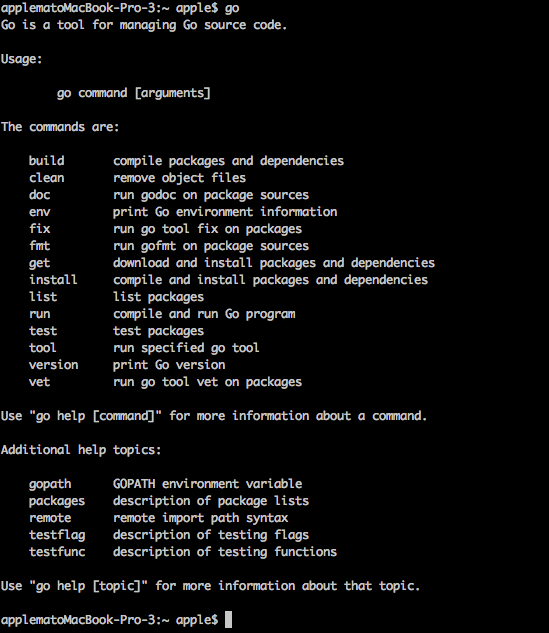
\includegraphics[width=14cm]{1.1.mac.png}
\label{図1.1}
\caption{ソースコードインストール後Goコマンドを実行}
\end{figure}

GoのUsage情報が表示されれば、Goのインストールは成功です:もしこのコマンドが存在しない場合は、PATH環境変数のなかにGoのインストールディレクトリが含まれているか確認してください。

\begin{quote}
  GOPATHについては以降の章で詳しくご説明します
\end{quote}




\subsubsection{Go標準パッケージのインストール}
Goはさまざまなプラットホームでインストールパッケージを提供しています、これらのパッケージはデフォルトで以下のディレクトリにインストールします:\//usr\//local\//go(Windows:c:$\backslash$ Go)。当然これらのインストール場所を変更することもできます、ただし変更後はあなたの環境変数を以下のように設定する必要があります:

\begin{lstlisting}[numbers=none]
export GOROOT=$HOME/go
export GOPATH=$HOME/gopath
export PATH=$PATH:$GOROOT/bin:$GOPATH/bin
\end{lstlisting}


これらのコマンドはMacやUnixユーザであれば\texttt{.bashrc}や\texttt{.zshrc}ファイルに入れておくべきでしょう。Windowsユーザであれば当然環境変数に入れておきます。

\subsubsection{自分の操作しているシステムが32bitか64bitか判断する方法}
Goのインストールにはオペレーティングシステムのbit数を判断する必要があるので、この章では先に自分のシステムの種類を確認しましょう。

WindowsのユーザはWin+Rを押してcmdを実行してください。\texttt{systeminfo}と入力してエンターキーを押します。しばらくするとシステムの情報が表示されます。"システムの種類"の一行に"x64-based PC"と表示されていれば64bitシステムです。もし"X86-based PC"とあれば、32bitシステムです。

Macユーザは直接64bit版を使用することをおすすめします。GoがサポートしているMac OS Xのバージョンは、すでに32bitプロセッサをサポートしていないためです。

LinuxユーザはTerminalで\texttt{arch}(すなわち、\texttt{uname -a})を実行することでシステムの情報を確かめることができます。

64bitシステムであれば以下のように表示されます。

\begin{lstlisting}[numbers=none]
x86_64
\end{lstlisting}

32bitシステムの場合は以下のように表示されます。

\begin{lstlisting}[numbers=none]
i386
\end{lstlisting}

\subsubsection{Mac インストール}
ダウンロードURLにアクセスし、32bitシステムはgo1.4.2.darwin-386-osx10.8.pkgをダウンロードします。64bitシステムであればgo1.4.2.darwin-amd64-osx10.8.pkgをダウンロードします。ファイルをダブルクリックし、すべてデフォルトで「次へ」ボタンをクリックします。これでgoはあなたのシステムにインストールされました。デフォルトでPATHの中に適切な\texttt{~\//go\//bin}が追加されています。端末を開いて\texttt{go}と入力します。

インストール成功の画像が表示されればインストール成功です。

もしgoのUsage情報が表示した場合は、goはすでにインストールされています。もしこのコマンドが存在しないと表示した場合は、自分のPATH環境変数の中にgoのインストールディレクトリが含まれているか確認してください。


\subsubsection{Linux インストール}
ダウンロードURLにアクセスし、32bitシステムであればgo1.4.2.linux-386.tar.gzを、64bitシステムであればgo1.2.2.linux-amd64.tar.gzをダウンロードします。

以下ではGoがインストールされたディレクトリを\texttt{\$GO\_INSTALL\_DIR}と仮定します。

\texttt{tar.gz}をインストールディレクトリに解凍します:\texttt{tar zxvf go1.4.2.linux-amd64.tar.gz -C \$GO\_INSTALL\_DIR}

PATHを設定します。\texttt{export PATH=\$PATH:\$GO\_INSTALL\_DIR\//go\//bin}

その後、\texttt{go}を実行します。

\begin{figure}[H]
  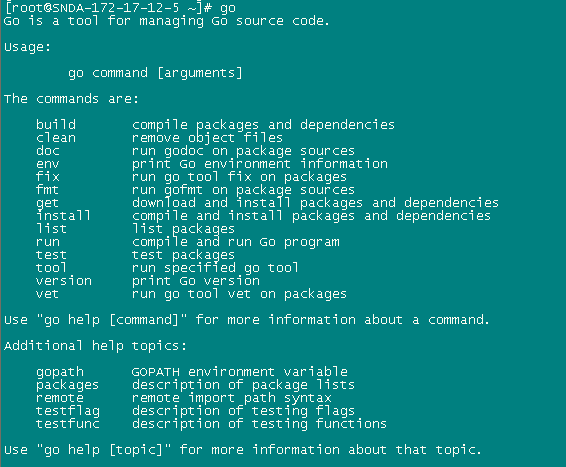
\includegraphics[width=14cm]{1.1.linux.png}
   \label{図1.2}
   \caption{Linuxシステムでインストールに成功したあとgoを実行した時に表示する情報}
\end{figure}

もしgoのUsage情報が表示された場合は、goはすでにインストールされています。もしこのコマンドが存在しないと出てきた場合は、自分のPATH環境変数の中にgoのインストールディレクトリが含まれているか確認してください。


\subsubsection{Windows インストール}
Google Code ダウンロードページ(http:\//\//golang.org\//dl\//)にアクセスし、32bit の場合は名前に windows-386 を含む msi パッケージを、64bit であれば名前に windows-amd64 を含むものをダウンロードします。ダウンロード後実行しますが、デフォルトのインストールフォルダである C:$\backslash$ Go$\backslash$を変更してはいけません。他の場所にインストールしてしまうと、あなたが書いた Go コードが実行できなくなってしまうかもしれません。インストールが終わるとデフォルトで環境変数 Path に Go のインストールフォルダの下にある bin フォルダ $C:\backslash Go\backslash bin\backslash$ が追加され、Go のインストールフォルダである $C:\backslash Go\backslash$ の値が環境変数 GOROOT に追加されます。

\paragraph{インストールが成功しているか確認する}


「ファイル名を指定して実行」に \texttt{cmd} を入力し、コマンドラインツールを開きます。プロンプトで\texttt{go}と入力することで Usage 情報が確認できるか確かめることができます。\texttt{cd \%GOROOT\%} を入力すると、Go のインストールフォルダに入れるか確認できます。どちらも成功していれば、インストールに成功しています。

インストールに成功していなければ、環境変数 Path と GOROOT の値を確認してください。もし存在しなければアンインストールの上再インストールし、存在していればコンピュータを再起動し、上の手順を再度試してください。


\subsubsection{サードパーティツールのインストール}
\paragraph{GVM}
gvmはサードパーティが開発したGoのバージョン管理ツールです。rubyのrvmツールに似ています。相当使い勝手がいいです。gvmをインストールするには以下のコマンド実行します:

\begin{lstlisting}[numbers=none]
bash < <(curl -s -S -L https://raw.github.com/moovweb
/gvm/master/binscripts/gvm-installer)
\end{lstlisting}

インストールが完了したあと、goをインストールすることができます:

\begin{lstlisting}[numbers=none]
gvm install go1.4.2
gvm use go1.4.2
\end{lstlisting}

下のコマンドで、毎回gvm useをコールする手間を省くことができます: gvm use go1.4.2 --default

上のコマンドを実行したあと、GOPATH、GOROOTなどの環境変数が自動的に設定されます。これで、直接利用することができます。

\paragraph{apt-get}
Ubuntuは現在最も多く利用されているLinuxデスクトップシステムです。\texttt{apt-get}コマンドでソフトウェア・パッケージを管理します。下のコマンドでGoをインストールすることができます、今後のため\texttt{git}と\texttt{mercurial}もインストールしておくべきでしょう:

\begin{lstlisting}[numbers=none]
sudo apt-get install python-software-properties
sudo add-apt-repository ppa:gophers/go
sudo apt-get update
sudo apt-get install golang-stable git-core mercurial
\end{lstlisting}

\paragraph{homebrew}
homebrewはMacで現在最も使用されているソフトウェア管理ツールです。現在Goをサポートしており、以下のコマンドでGoを直接インストールすることができます。今後のため\texttt{git}と\texttt{mercurial}もインストールしておくべきでしょう:

\begin{lstlisting}[numbers=none]
brew update && brew upgrade
brew install go
brew install git
brew install mercurial
\end{lstlisting}



\subsection{GOPATHとワーキングディレクトリ}
さきほどGoをインストールする際はGOPATH変数を設定する必要があるとご説明しました。Goはバージョン1.1から必ずこの変数を設定するようになっており、Goのインストールディレクトリと同じにはできません。このディレクトリは、GoのソースコードやGoの実行可能ファイル、並びにコンパイル済みのパッケージファイルを保存する為に使用します。そのためこのディレクトリには3つのサブディレクトリが存在します:src、bin、pkgです。

\subsubsection{GOPATH設定}
 go コマンドは、ある重要な環境変数に依存しています:\$GOPATH

Windowsシステムにおいて環境変数の形式は\texttt{\%GOPATH\%}です。この本の中では主にUnix形式を使用します。Windowsユーザは適時置き換えてください。

(注:これはGoのインストールディレクトリではありません。以下では筆者のワーキングディレクトリで説明します。もし異なるディレクトリを使用する場合はGOPATHをあなたのワーキングディレクトリに置き換えてください。)

Unix に似た環境であれば大体以下のような設定になります:

\begin{lstlisting}[numbers=none]
export GOPATH=/home/apple/mygo
\end{lstlisting}

 上のディレクトリを新たに作成し、上の一行を\texttt{.bashrc}または\texttt{.zshrc}もしくは自分のshの設定ファイルに加えます。

 Windows では以下のように設定します。新しくGOPATHと呼ばれる環境変数を作成します:

\begin{lstlisting}[numbers=none]
  GOPATH=c:\mygo
\end{lstlisting}

GOPATHは複数のディレクトリを許容します。複数のディレクトリがある場合、デリミタに気をつけてください。複数のディレクトリがある場合Windowsはセミコロン、Linuxはコロンを使います。複数のGOPATHがある場合は、デフォルトでgo getの内容が第一ディレクトリとされます。

上の \$GOPATH ディレクトリには3つのディレクトリがあります:

\begin{itemize}
  \item src にはソースコードを保存します(例えば:.go .c .h .s等)
  \item pkg にはコンパイル後に生成されるファイル(例えば:.a)
  \item bin にはコンパイル後に生成される実行可能ファイル(このまま \$PATH 変数に加えてもかまいません。もしいくつもgopathがある場合は、\texttt{\$\{GOPATH\//\//:\//\//bin:\}\//bin}を使って全てのbinディレクトリを追加してください)
\end{itemize}

以降私はすべての例でmygoを私のgopathディレクトリとします。

\subsubsection{ソースコードディレクトリ構成}
GOPATH内のsrcディレクトリはこれから開発するプログラムにとってメインとなるディレクトリです。全てのソースコードはこのディレクトリに置くことになります。一般的な方法では一つのプロジェクトが一つのディレクトリが割り当てられます、例えば:\$GOPATH\//src\//mymath はmymathというアプリケーションパッケージか実行アプリケーションになります。これはpackageがmainかそうでないかによって決定します。mainであれば実行可能アプリケーションで、そうでなければアプリケーションパッケージになります。これに関してはpackageを後ほどご紹介する予定です。

新しくアプリケーションやソースパッケージを作成するときは、srcディレクトリの中にディレクトリを作るところから始めます。ディレクトリ名は一般的にソースパッケージ名になります。もちろんネストしたディレクトリも可能です。例えばsrcの中に\$GOPATH\//src\//github.com\//astaxie\//beedbというディレクトリを作ったとすると、このパッケージパスは"github.com\//astaxie\//beedb"になり、パッケージ名は最後のディレクトリであるbeedbになります。

以下ではmymathを例にどのようにアプリケーションパッケージをコーディングするかご説明します。以下のコードを実行します。


\begin{lstlisting}[numbers=none]
cd $GOPATH/src
mkdir mymath
\end{lstlisting}



\begin{lstlisting}[numbers=none]
// $GOPATH/src/mymath/sqrt.goコードは以下の通り:
package mymath

func Sqrt(x float64) float64 {
    z := 0.0
    for i := 0; i < 1000; i++ {
        z -= (z*z - x) / (2 * x)
    }
    return z
}
\end{lstlisting}


このように私のアプリケーションパッケージディレクトリとコードが作成されました。注意:一般的にpackageの名前とディレクトリ名は一致させるべきです。


\subsubsection{コンパイルアプリケーション}
上のとおり、我々はすでに自分のアプリケーションパッケージを作成しましたが、どのようにコンパイル/インストールすべきでしょうか?2種類の方法が存在します。

\begin{enumerate}
  \item 対応するアプリケーションパッケージディレクトリに入り、\texttt{go install}を実行すればインストールできます。
  \item 任意のディレクトリで以下のコード\texttt{go install mymath}を実行します。
\end{enumerate}

インストールが終われば、以下のディレクトリに入り

\begin{lstlisting}[numbers=none]
cd $GOPATH/src
mkdir mathapp
cd mathapp
vim main.go
\end{lstlisting}

\$GOPATH\//src\//mathapp\//main.goコード:

\begin{lstlisting}[numbers=none]
package main

import (
      "mymath"
      "fmt"
)

func main() {
      fmt.Printf("Hello, world.  Sqrt(2) = %v\n", mymath.Sqrt(2))
}
\end{lstlisting}

このパッケージは\texttt{main}であることが分かると思います。importにおいてコールするパッケージは\texttt{mymath}であり、これが\texttt{\$GOPATH\//src}のパスに対応します。もしネストしたディレクトリであれば、importの中でネストしたディレクトリをインポートします。例えばいくつものGOPATHがあった場合も同じで、Goは自動的に複数の\texttt{\$GOPATH\//src}の中から探し出します。

さて、どのようにプログラムをコンパイルするのでしょうか?このアプリケーションディレクトリに入り、\texttt{go build}を実行すれば、このディレクトリの下にmathappの実行可能ファイルが生成されます。

\begin{lstlisting}[numbers=none]
./mathapp
\end{lstlisting}

以下のように出力されます。

\begin{lstlisting}[numbers=none]
Hello, world.  Sqrt(2) = 1.414213562373095
\end{lstlisting}

どのようにアプリケーションをインストールするのでしょうか。このディレクトリに入り、\texttt{go install}を実行すると、\$GOPATH\//bin\//の下に実行可能ファイルmathappが作成されます。\texttt{\$GOPATH\//bin}が我々のPATHに追加されていることを思い出して下さい、コマンドラインから以下のように入力することで実行することができます。

\begin{lstlisting}[numbers=none]
mathapp
\end{lstlisting}

この場合も以下のように出力されます。

\begin{lstlisting}[numbers=none]
Hello, world.  Sqrt(2) = 1.414213562373095
\end{lstlisting}

ここではどのように実行可能アプリケーションをコンパイル/インストールし、ディレクトリ構造を設計するかについてご紹介しました。





\subsubsection{リモートパッケージの取得}
go言語はリモートパッケージを取得するツール\texttt{go get}を持っています。現在go getは多数のオープンソースリポジトリをサポートしています(github、googlecode、bitbucket、Launchpad)

\begin{lstlisting}[numbers=none]
go get github.com/astaxie/beedb
\end{lstlisting}

\begin{quote}
go get -u オプションはパッケージの自動更新を行います。また、go get時に自動的に当該のパッケージの依存する他のサードパーティパッケージを取得します。
\end{quote}

このコマンドでふさわしいコードを取得し、対応するオープンソースプラットホームに対し異なるソースコントロールツールを利用します。例えばgithubではgit、googlecodeではhg。そのためこれらのコードを取得したい場合は、先に対応するソースコードコントロールツールをインストールしておく必要があります。

上述の方法で取得したコードはローカルの以下の場所に配置されます。

\begin{lstlisting}[numbers=none]
$GOPATH
  src
   |--github.com
          |-astaxie
              |-beedb
   pkg
    |--対応プラットフォーム
         |-github.com
               |--astaxie
                    |beedb.a
\end{lstlisting}

go getは以下のような手順を踏みます。まずはじめにソースコードツールでコードをsrcの下にcloneします。その後\texttt{go install}を実行します。

コードの中でリモートパッケージが使用される場合、単純にローカルのパッケージと同じように頭のimportに対応するパスを添えるだけです。



\begin{lstlisting}[numbers=none]
import "github.com/astaxie/beedb"
\end{lstlisting}



\subsubsection{プログラムの全体構成}
上記で作成したローカルのmygoのディレクトリ構造は以下のようになっています。


\begin{lstlisting}[numbers=none]
bin/
    mathapp
pkg/
    プラットフォーム名/ 例:darwin_amd64、linux_amd64
         mymath.a
         github.com/
              astaxie/
                   beedb.a
src/
    mathapp
          main.go
      mymath/
          sqrt.go
      github.com/
           astaxie/
                beedb/
                    beedb.go
                    util.go
\end{lstlisting}


上述の構成から明確に判断できるのは、binディレクトリの下にコンパイル後の実行可能ファイルが保存され、pkgの下に関数パッケージが保存され、srcの下にアプリケーションのソースコードが保存されているということです。




\subsection{Goのコマンド}
\subsubsection{Goのコマンド}
Go言語は完全なコマンド操作ツールセットを持つ言語です。コマンドラインでgoを実行することでそれらを確認することができます:

\begin{figure}[H]
   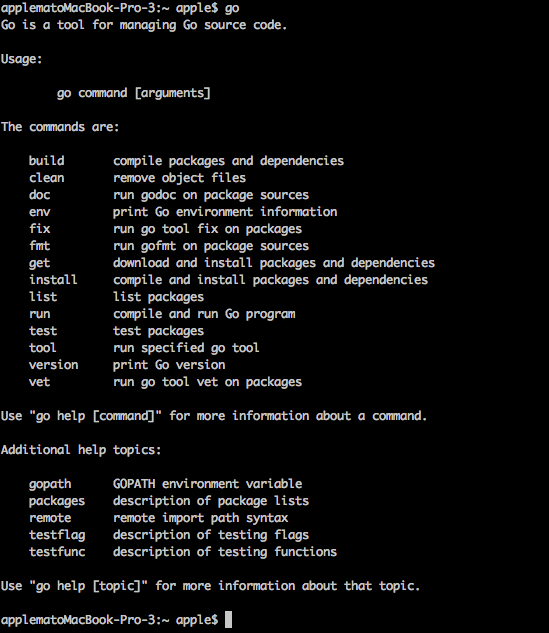
\includegraphics[width=14cm]{1.1.mac.png}
   \label{図1.3}
   \caption{Goコマンドで詳細情報を表示}
\end{figure}

これらのコマンドは我々が普段コードを書いている時に非常に役立つものです。次に普段使用するコマンドを理解していきましょう。

\subsubsection{go build}
このコマンドは主にソースコードのコンパイルに用いられます。パッケージのコンパイル作業中、もし必要であれば、同時に関連パッケージもコンパイルすることができます。

\begin{itemize}
  \item もし普通のパッケージであれば、我々が1.2章で書いた\texttt{mypath}パッケージのように、\texttt{go build}を実行したあと、何のファイルも生成しません。もし\texttt{\$GOPATH\//pkg}の下に対応するファイルを生成する必要があれば、\texttt{go install}を実行してください。
  \item もしそれが\texttt{main}パッケージであれば、\texttt{go build}を実行したあと、カレントディレクトリの下に実行可能ファイルが生成されます。もし\texttt{\$GOPATH\//bin}の下に対応するファイルを生成する必要があれば、\texttt{go install}を実行するか、\texttt{go build -o パス\//a.exe}を実行してください。
  \item もしあるプロジェクトディレクトリに複数のファイルがある場合で、単一のファイルのみコンパイルしたい場合は、\texttt{go build}を実行する際にファイル名を追加することができます。例えば\texttt{go build a.go}です。\texttt{go build}コマンドはデフォルトでカレントディレクトリにある全てのgoファイルをコンパイルしようと試みます。
  \item コンパイル後に出力されるファイル名を指定することもできます。1.2章の\texttt{mathapp}アプリケーションでは\texttt{go build -o astaxie.exe}と指定できます。デフォルトはpackage名(mainパッケージではない)になるか、ソースファイルのファイル名(mainパッケージ)になります。\\(注:実際はpackage名はGo言語の規格においてコード中の"package"に続く名前になります。この名前はファイル名と異なっていても構いません。デフォルトで生成される実行可能ファイル名はディレクトリ名。
  \item go buildはディレクトリ内の"\_"または"."ではじまるgoファイルを無視します。
  \item もしあなたのソースコードが異なるオペレーティングシステムに対応する場合は異なる処理が必要となります。ですので異なるオペレーティングシステムの名称にもとづいてファイルを命名することができます。例えば配列を読み込むプログラムがあったとして、異なるオペレーティングシステムに対して以下のようなソースファイルがあるかもしれません。\\array\_linux.go array\_darwin.go array\_windows.go array\_freebsd.go\\go buildの際、システム名の末尾のファイルから選択的にコンパイルすることができます(Linux、Darwin、Windows、Freebsd)
\end{itemize}

引数の紹介

\begin{description}
  \item[-o] 出力するファイル名を指定します。パスが含まれていても構いません。例えば \texttt{go build -o a\//b\//c}
  \item[-i] パッケージをインストールします。コンパイル+\texttt{go install}
  \item[-a] すでに最新であるパッケージを全て更新します。ただし標準パッケージには適用されません。
  \item[-n] 実行が必要なコンパイルコマンドを出力します。ただし、実行はされません。これにより低レイヤーで一体何が実行されているのかを簡単に知る事ができます。
  \item[-p n] マルチプロセスで実行可能なコンパイル数を指定します。デフォルトはCPU数です。
  \item[-race] コンパイルを行う際にレースコンディションの自動検出を行います。64bitマシンでのみ対応しています。
  \item[-v] 現在コンパイル中のパッケージ名を出力します。
  \item[-work] コンパイル時の一時ディレクトリ名を出力し、すでに存在する場合は削除しなくなります。
  \item[-x] 実行しているコマンドを出力します。\texttt{-n}の結果とよく似ていますが、この場合は実行します。
  \item[-ccflags 'arg list'] オプションを5c, 6c, 8cに渡してコールします。
  \item[-compiler name] コンパイラを指定します。gccgoか、またはgcです。
  \item[-gccgoflags 'arg list'] オプションをgccgoリンカに渡してコールします。
  \item[-gcflags 'arg list'] オプションを5g, 6g, 8gに渡してコールします
  \item[-installsuffix suffix] デフォルトのインストールパッケージと区別するため、このサフィックスを利用して依存するパッケージをインストールします。\texttt{-race}をオプションに指定した場合はデフォルトで\texttt{-installsuffix race}が有効になっています。\texttt{-n}コマンドで確かめることができますよ。
  \item[-ldflags 'flag list'] オプションを5l, 6l, 8lに渡してコールします。
  \item[-tags 'tag list'] コンパイル時にこれらのtagをつけることができます。tagの詳細な制限事項に関しては Build Constraints(http:\//\//golang.org\//pkg\//go\//build\//) を参考にして下さい。
\end{description}

\subsubsection{go clean}
 このコマンドは現在のソースコードパッケージと関連するソースパッケージのなかでコンパイラが生成したファイルを取り除く操作を行います。これらのファイルはすなわち:


\begin{lstlisting}[numbers=none]
_obj/            旧objectディレクトリ、MakeFilesが作成する。
_test/           旧testディレクトリ,Makefilesが作成する。
_testmain.go     旧gotestファイル,Makefilesが作成する。
test.out         旧testログ,Makefilesが作成する。
build.out        旧testログ,Makefilesが作成する。
*.[568ao]        objectファイル,Makefilesが作成する。

DIR(.exe)        go buildが作成する。
DIR.test(.exe)   go test -cが作成する。
MAINFILE(.exe)   go build MAINFILE.goが作成する。
*.so             SWIG によって生成される。
\end{lstlisting}

私は基本的にこのコマンドを使ってコンパイルファイルを掃除します。ローカルでテストを行う場合これらのコンパイルファイルはシステムと関係があるだけで、コードの管理には必要ありません。

\begin{lstlisting}[numbers=none]
$ go clean -i -n
cd /Users/astaxie/develop/gopath/src/mathapp
rm -f mathapp mathapp.exe mathapp.test mathapp.test.exe app app.exe
rm -f /Users/astaxie/develop/gopath/bin/mathapp
\end{lstlisting}

引数紹介

\begin{description}
  \item[-i] go installがインストールするファイル等の、関係するインストールパッケージと実行可能ファイルを取り除きます。
  \item[-n] 実行する必要のある削除コマンドを出力します。ただし実行はされません。これにより低レイヤで何が実行されているのかを簡単に知ることができます。
  \item[-r] importによってインポートされたパッケージを再帰的に削除します。
  \item[-x] 実行される詳細なコマンドを出力します。\texttt{-n}出力の実行版です。
\end{description}

\subsubsection{go fmt}
 読者にC\//C++の経験があればご存知かもしれませんが、コードにK\&Rスタイルを選択するかANSIスタイルを選択するかは常に論争となっていました。goでは、コードに標準のスタイルがあります。すでに培われた習慣やその他が原因となって我々は常にANSIスタイルまたはその他のより自分にあったスタイルでコードを書いて来ました。これは他の人がコードを閲覧する際に不必要な負担を与えます。そのためgoはコードのスタイルを強制し(例えば左大括弧はかならず行末に置く)、このスタイルに従わなければコンパイルが通りません。整形の時間の節約するため、goツールは\texttt{go fmt}コマンドを提供しています。これはあなたの書いたコードを整形するのに役立ちます。あなたの書いたコードは標準のスタイルに修正されますが、我々は普段このコマンドを使いません。なぜなら開発ツールには一般的に保存時に自動的に整形を行ってくれるからです。この機能は実際には低レイヤでは\texttt{go fmt}を呼んでいます。この次の章で2つのツールをご紹介しましょう。この2つのツールはどれもファイルを保存する際に\texttt{go fmt}機能を自動化させます。

go fmtコマンドを使うにあたって実際にはgofmtがコールされますが、-wオプションが必要になります。さもなければ、整形結果はファイルに書き込まれません。gofmt -w -l src、ですべての項目を整形することができます。

go fmtはgofmtの上位レイヤーのパッケージされたコマンドです。より個人的なフォーマットスタイルが欲しい場合は \texttt{gofmt}(http:\//\//golang.org\//cmd\//gofmt\//) を参考にしてください。

gofmtの引数紹介

\begin{description}
  \item[-l] フォーマットする必要のあるファイルを表示します。
  \item[-w] 修正された内容を標準出力に書き出すのではなく、直接そのままファイルに書き込みます。
  \item[-r] “a[b:len(a)] -$>$ a[b:]”のような重複したルールを追加します。大量に変換を行う際に便利です。
  \item[-s] ファイルのソースコードを簡素化します。
  \item[-d] ファイルに書き込まず、フォーマット前後のdiffを表示します。デフォルトはfalseです。
  \item[-e] 全ての文法エラーを標準出力に書き出します。もしこのラベルを使わなかった場合は異なる10行のエラーまでしか表示しません。
  \item[-cpuprofile] テストモードをサポートします。対応するするcpufile指定のファイルに書き出します。
\end{description}

\subsubsection{go get}
このコマンドは動的にリモートコードパッケージを取得するために用いられます。現在BitBucket、GitHub、Google CodeとLaunchpadをサポートしています。このコマンドは内部で実際には2ステップの操作に分かれます:第1ステップはソースコードパッケージのダウンロード、第2ステップは\texttt{go install}の実行です。ソースコードパッケージのダウンロードを行うgoツールは異なるドメインにしたがって自動的に異なるコードツールを用います。対応関係は以下の通りです:

\begin{lstlisting}[numbers=none]
BitBucket (Mercurial Git)
GitHub (Git)
Google Code Project Hosting (Git, Mercurial, Subversion)
Launchpad (Bazaar)
\end{lstlisting}

 そのため、\texttt{go get}を正常に動作させるためには、あらかじめ適切なソースコード管理ツールがインストールされていると同時にこれらのコマンドがあなたのPATHに入っていなければなりません。実は\texttt{go get}はカスタムドメインの機能をサポートしています。具体的な内容は\texttt{go help remote}を参照ください。

引数紹介:

\begin{description}
  \item[-d] ダウンロードするだけでインストールしません。
  \item[-f] \texttt{-u}オプションを与えた時だけ有効になります。\texttt{-u}オプションはimportの中の各パッケージが既に取得されているかを検証しなくなります。ローカルにforkしたパッケージに対して特に便利です。
  \item[-fix] ソースコードをダウンロードするとまずfixを実行してから他の事を行うようになります。
  \item[-t] テストを実行する為に必要となるパッケージも同時にダウンロードします。
  \item[-u] パッケージとその依存パッケージをネットワークから強制的に更新します。
  \item[-v] 実行しているコマンドを表示します。
\end{description}

\subsubsection{go install}
 このコマンドは実際には内部で2ステップの操作に分かれます。第1ステップはリザルトファイルの生成(実行可能ファイルまたはaパッケージ)、第2ステップはコンパイルし終わった結果を\texttt{\$GOPATH\//pkg}または\texttt{\$GOPATH\//bin}に移動する操作です。

 引数は\texttt{go build}のコンパイルオプションをサポートしています。みなさんは\texttt{-v}オプションだけ覚えていただければ結構です。これにより低レイヤーの実行状況をいつでも確認することができます。
 

\subsubsection{go test}
このコマンドを実行すると、ソースコードディレクトリ以下の\texttt{*\_test.go}ファイルが自動的にロードされ、テスト用の実行可能ファイルが生成/実行されます。出力される情報は以下のようなものになります


\begin{lstlisting}[numbers=none]
ok   archive/tar   0.011s
FAIL archive/zip   0.022s
ok   compress/gzip 0.033s
...
\end{lstlisting}

 デフォルトの状態で、オプションを追加する必要はありません。自動的にあなたのソースコードパッケージ以下のすべてのtestファイルがテストされます。もちろんオプションを追加しても構いません。詳細は\texttt{go help testflag}を確認してください。

ここでは良く使われるオプションについてご紹介します:

\begin{description}
  \item[-bench regexp] 指定したbenchmarksを実行します。例えば \texttt{-bench=.}
  \item[-cover] テストカバー率を起動します。
  \item[-run regexp] regexpにマッチする関数だけを実行します。例えば \texttt{-run=Array} とすることで名前がArrayから始まる関数だけを実行します。
  \item[-v] テストの詳細なコマンドを表示します。
\end{description}


\subsubsection{go tool}
\texttt{go tool}にはいくつものコマンドがあります。ここでは2つだけご紹介します。fixと vetです。


\begin{itemize}
  \item \texttt{go tool fix .} は以前の古いバージョンを新しいバージョンに修復します。例えば、go1以前の古いバージョンのコードをgo1に焼き直したり、APIを変化させるといったことです。
  \item \texttt{go tool vet directory|files} はカレントディレクトリのコードが正しいコードであるか分析するために使用されます。例えばfmt.Printfをコールする際のオプションが正しくなかったり、関数の途中でreturnされたことによって到達不可能なコードが残っていないかといった事です。
\end{itemize}

\subsubsection{go generate}
このコマンドはGo1.4になって初めてデザインされました。コンパイル前にある種のコードを自動で生成する目的に使用されます。\texttt{go generate}と\texttt{go build}は全く異なるコマンドです。ソースコード中の特殊なコメントをを分析することで、対応するコマンドを実行します。これらのコマンドは明確に何の依存も存在しません。この機能を使用する場合には必ず次の事を念頭に置いてください。\texttt{go generate}はあなたの為に存在します。あなたのパッケージを使用する誰かの為のものではありません。これはある一定のコードを生成するためにあります。

簡単な例をご紹介します。例えば我々が度々\texttt{yacc}を使ってコードを生成していたとしましょう。その場合以下のようなコマンドをいつも使用することになります:


\begin{lstlisting}[numbers=none]
go tool yacc -o gopher.go -p parser gopher.y
\end{lstlisting}

-o は出力するファイル名を指定します。-pはパッケージ名を指定します。これは単独のコマンドであり、もし\texttt{go generate}によってこのコマンドを実行する場合は当然ディレクトリの任意の\texttt{xxx.go}ファイルの任意の位置に以下のコメントを一行追加します。

\begin{lstlisting}[numbers=none]
//go:generate go tool yacc -o gopher.go -p parser gopher.y
\end{lstlisting}

注意すべきは、\texttt{\//\//go:generate}に空白が含まれていない点です。これは固定のフォーマットで、ソースファイルを舐める時はこのフォーマットに従って判断されます。

これにより以下のようなコマンドによって、生成・コンパイル・テストを行うことができます。もし\texttt{gopher.y}ファイルに修正が発生した場合は、再度\texttt{go generate}を実行することでファイルを上書きすればよいことになります。

\begin{lstlisting}[numbers=none]
$ go generate
$ go build
$ go test
\end{lstlisting}




\subsubsection{godoc}
Go1.2バージョンより以前は\texttt{go doc}コマンドがサポートされていましたが、今後は全てgodocコマンドに移されました。このようにインストールします\texttt{go get golang.org\//x\//tools\//cmd\//godoc}

多くの人がgoにはサードパーティのドキュメントが必要無いと謳っています。なぜなら例えばchmハンドブックのように(もっとも私はすでにchmマニュアルを作っていますが)、この中にはとても強力なドキュメントツールが含まれているからです。

どのように対応するpackageのドキュメントを確認すればよいでしょうか? 例えばbuiltinパッケージであれば、\texttt{go doc builtin}と実行します。 もしhttpパッケージであれば、\texttt{go doc net\//http}と実行してください。 パッケージの中の関数を確認する場合は\texttt{godoc fmt Printf}としてください。 対応するコードを確認する場合は、\texttt{godoc -src fmt Printf}とします。

コマンドラインでコマンドを実行します。 godoc -http=:ポート番号 例えば\texttt{godoc -http=:8080}として、ブラウザで\texttt{127.0.0.1:8080}を開くと、golang.orgのローカルのcopy版を見ることができます。これを通してpkgドキュメントなどの他の内容を確認することができます。もしあなたがGOPATHを設定されていれば、pkgカテゴリの中で、標準パッケージのドキュメントのみならず、ローカルの\texttt{GOPATH}のすべての項目に関連するドキュメントをリストアップすることができます。これはグレートファイアーウォールの中にいるユーザにとっては非常にありがたい選択です。

\subsubsection{その他のコマンド}
 goは他にも様々なツールを提供しています。例えば以下のツール

\begin{lstlisting}[numbers=none]
go version はgoの現在のバージョンを確認します。
go env は現在のgoの環境変数を確認します。
go list は現在インストールされている全てのpackageをリストアップします。
go run はGoプログラムのコンパイルと実行を行います。
\end{lstlisting}


これらのツールはまだ多くのオプションがあり、ひとつひとつはご紹介しませんが、ユーザは\texttt{go help コマンド}で更に詳しいヘルプ情報を取得することができます。


\subsection{Goの開発ツール}
本章ではいくつかの開発ツールをご紹介します。これらはすべて自動化を備えており、fmt機能を自動化します。なぜならこれらはすべてクロスプラットフォームであり、そのためインストール手順といったものはすべて同じものです。

\subsubsection{LiteIDE}
LiteIDEはGo言語の開発に特化したクロスプラットフォームの軽量統合開発環境(IDE)です。visualfcで書かれています。


\begin{figure}[H]
   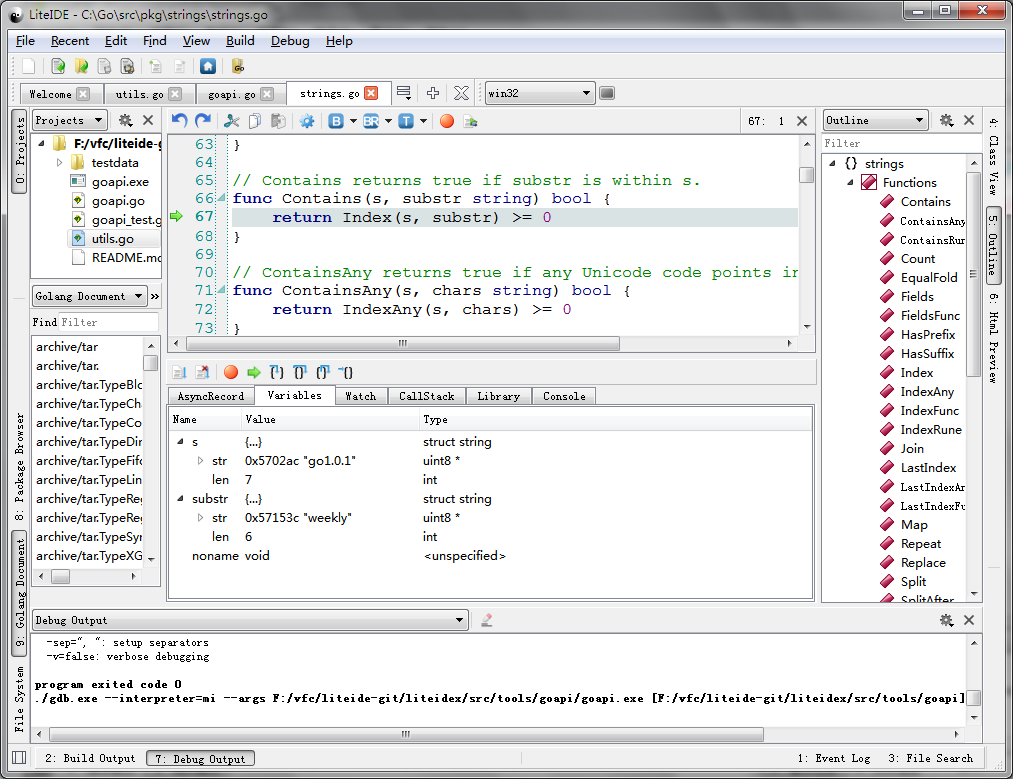
\includegraphics[width=14cm]{1.4.liteide.png}
   \label{図1.4}
   \caption{LiteIDEのメイン画面}
\end{figure}

\paragraph{LiteIDEの主な特徴}
\begin{itemize}
  \item 主なオペレーティングシステムのサポート
  \begin{itemize}
    \item Windows
    \item Linux
    \item MacOS X
  \end{itemize}

  \item Goコンパイル環境の管理と切り替え
    \begin{itemize}
    \item 複数のGoコンパイル環境の管理と切り替え
    \item Go言語のクロスコンパイルのサポート
    \end{itemize}

  \item Go標準と同じ項目管理方式
    \begin{itemize}
    \item GOPATHに基づいたパッケージブラウザ
    \item GOPATHに基づいたコンパイルシステム
    \item GOPATHに基づいたドキュメント検索
    \end{itemize}
  \item Go言語の編集サポート
    \begin{itemize}
    \item クラスブラウザとアウトライン表示
    \item Gocode(コード自動作成ツール)の完全なサポート
    \item Go言語ドキュメントとApi高速検索
    \item コード表現情報の表示\texttt{F1}
    \item ソースコード定義とジャンプのサポート\texttt{F2}
    \item Gdbブレークポイントとテストサポート
    \item gofmt自動整形のサポート
    \end{itemize}
  \item その他の特徴
    \begin{itemize}
    \item 多言語メニューのサポート
    \item 完全にプラガブルな構成
    \item エディタのカラーリングサポート
    \item Kateに基づいた文法表示サポート
    \item 全文に基づく単語の自動補完
    \item キーボードショートカットのバインディングサポート
    \item Markdownドキュメントの編集サポート
      \begin{itemize}
      \item リアルタイムプレビューと表示の同期
      \item カスタムCSS表示
      \item HTML及びPDFドキュメントのエクスポート
      \item HTML\//PDFドキュメントへの変換とマージ
      \end{itemize}
    \end{itemize}
\end{itemize}

\paragraph{LiteIDEインストール設定}
\begin{itemize}
  \item LiteIDEインストール
    \begin{itemize}
    \item ダウンロード http:\//\//sourceforge.net\//projects\//liteide\//files\//
    \item ソースコード https:\//\//github.com\//visualfc\//liteide
    \end{itemize}
  \item コンパイル環境設定
\begin{lstlisting}[numbers=none]
  自身のシステムの要求にしたがってLiteIDEが現在使用している
  環境変数を切り替えまたは設定します。

  Windowsオペレーティングシステムの64bitGo言語の場合、
  ツール欄の環境設定のなかでwin64を選択し、`編集環境`をクリック
  してLiteIDEからwin64.envファイルを編集します。

  GOROOT=c:\go
  GOBIN=
  GOARCH=amd64
  GOOS=windows
  CGO_ENABLED=1

  PATH=%GOBIN%;%GOROOT%\bin;%PATH%
  。。。

  この中の`GOROOT=c:\go`を現在のGoのインストールパスに修正し、
  保存するだけです。もしMinGW64があれば、`c:\MinGW64\bin`を
  PATHの中に入れて、goによるgccのコールでCGOコンパイラのサポートを
  利用することができます。

  Linuxオペレーティングシステムで64bitGo言語の場合、
  ツール欄の環境設定の中からlinux64を選び、`編集環境`をクリックし
  LiteIDEからlinux64.envファイルを編集します。

  GOROOT=$HOME/go
  GOBIN=
  GOARCH=amd64
  GOOS=linux
  CGO_ENABLED=1

  PATH=$GOBIN:$GOROOT/bin:$PATH    
  。。。

  この中の`GOROOT=$HOME/go`を現在のGoのインストールパスに
  修正して保存します。
\end{lstlisting}
  \item GOPATH設定
\begin{lstlisting}[numbers=none]
  Go言語のツールキーはGOPATH設定を使用します。Go言語開発の
  プロジェクトのパスリストです。コマンドライン(LiteIDEでは
  `Ctrl+,`を直接入力できます)で`go help gopath`を入力する
  とGOPATHドキュメントを素早く確認できます。

  LiteIDEでは簡単に確認でき、GOPATHを設定することができます。
  `メニュー-確認-GOPATH`設定を通じて、システム中に存在する
  GOPATHリストを確認することができます。
  同時に必要な追加項目にそってカスタムのGOPATHリストに追加
  することができます。
\end{lstlisting}
\end{itemize}

\subsubsection{Sublime Text}
ここではSublime Text 2(以下「Sublime」)+GoSublimeの組み合わせをご紹介します。なぜこの組み合わせなのでしょうか?


\begin{itemize}
  \item コード表示の自動化、以下の図の通り\\ 
\begin{figure}[H]
  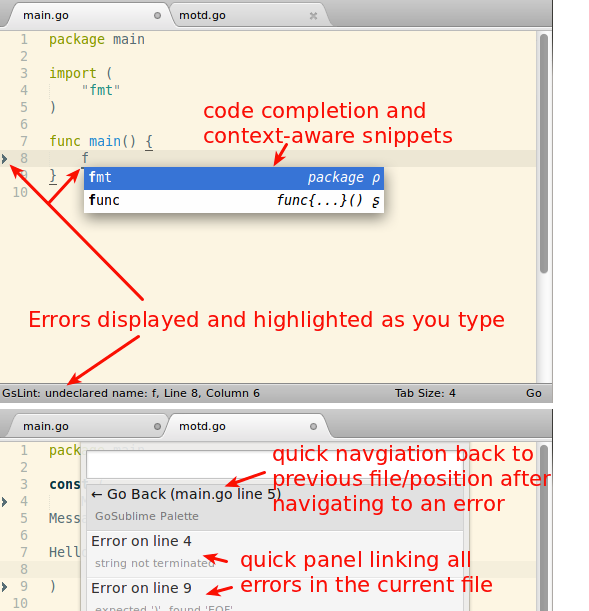
\includegraphics[width=14cm]{1.4.sublime1.png}
   \label{図1.5}
   \caption{sublimeコードの自動化画面}
\end{figure}
  \item 保存した時にはコードが自動的に整形されています。あなたの書いたコードをより美しくGoの標準に合うよう仕上げてくれます。
  \item プロジェクト管理のサポート\\ 
\begin{figure}[H]
  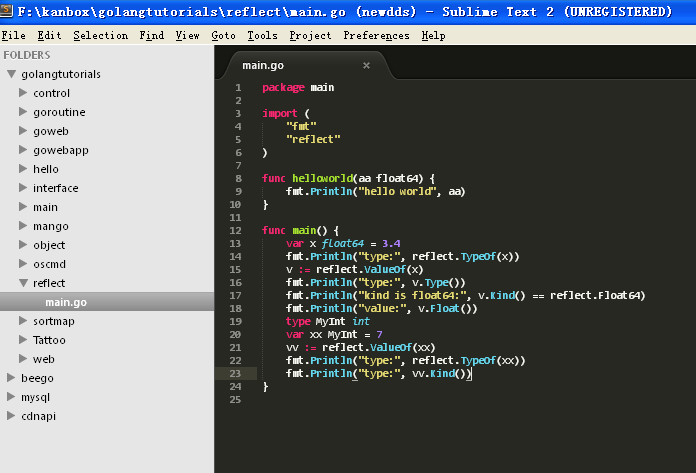
\includegraphics[width=14cm]{1.4.sublime2.png}
   \label{図1.6}
   \caption{sublimeプロジェクト管理画面}
\end{figure}
  \item 文法のハイライトサポート
  \item Sublime Text 2はフリーで使用できます。保存回数が一定の量を超えると購入するかのダイアログが現れるので、継続利用をキャンセルするをクリックします。正式登録版とは何の違いもありません。
\end{itemize}


次はどのようにインストールするかご説明します。Sublimeダウンロードします。

自分のシステムに合わせて対応するバージョンをダウンロードし、Sublimeを開きます。Sublimeに詳しくない方はまずSublime Text 2 入門とテクニック(http:\//\//lucifr.com\//139225\//sublime-text-2-tricks-and-tips\//)の文章を読んでみてください。

\begin{enumerate}
  \item 開いた後、 Package Controlをインストールします。Ctrl+`でコマンドラインを開き、以下のコードを実行します:
\begin{lstlisting}[numbers=none]
  import urllib2,os; pf='Package Control.sublime-package';
  ipp=sublime.installed_packages_path();
  os.makedirs(ipp) if not os.path.exists(ipp) else None;
  urllib2.install_opener(urllib2.build_opener(urllib2.ProxyHandler()));
  open(os.path.join(ipp,pf),'wb').write(
          urllib2.urlopen('http://sublime.wbond.net/'+pf.
          replace(' ','%20')).read());
  print 'Please restart Sublime Text to finish installation'
\end{lstlisting}
この時Sublimeを再度開き直してください。メニュー欄に一つ項目が増えているのがお分かりいただけるかと思います。これでPackage Controlが正しくインストールされました。\\ 
\begin{figure}[H]
  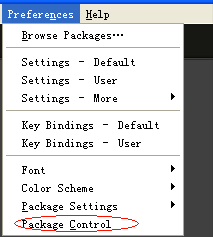
\includegraphics[width=8cm]{1.4.sublime3.png}
   \label{図1.7}
   \caption{sublimeパッケージ管理}
\end{figure}
  \item インストールが完了するとSublimeのプラグインをインストールできます。GoSublime, SidebarEnhancementsとGo Buildをインストールする必要があるので、プラグインをインストールしたあとSublimeを再起動させて有効にしてください。Ctrl+Shift+pでPackage Controlを開き、pcipを入力します。(これは"Package Control: Install Package"と省略されます)。\\ この時、左下のコーナーに現在読み込んでいるパッケージデータが表示されます。完了すると下のような画面になります。\\ 
\begin{figure}[H]
  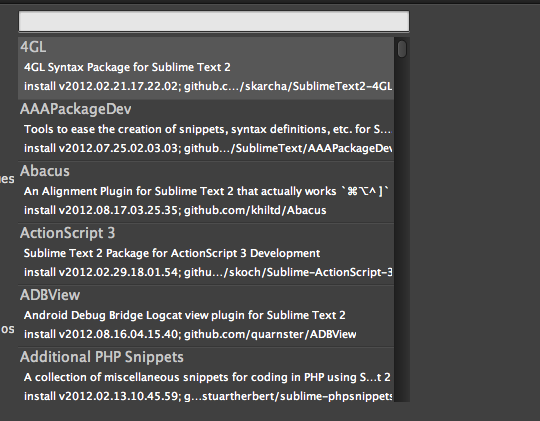
\includegraphics[width=14cm]{1.4.sublime4.png}
   \label{図1.8}
   \caption{sublimeプラグインのインストール画面}
\end{figure}
この時、GoSublimeと入力し、「確認」をクリックするとインストールが始まります。同じようにSidebarEnhancementsとGo Buildにも行います。
  \item インストールが成功したかテストします。Sublimeを開き、main.goを開いて文法がハイライトされているのをご確認ください。\texttt{import}を入力してコードの自動表示がされます。\texttt{import "fmt"}のあとに\texttt{fmt.}を入力すると自動的に関数の候補が現れます。\\ もしすでにこのような表示がされる場合は、インストールが成功しており、自動補完が完了しています。\\ もしこのような表示がなされない場合、あなたの\texttt{\$PATH}が正しく設定されていないのかもしれません。ターミナルを開き、gocodeを入力して、正しく実行できるか確認してください。もしダメであれば\texttt{\$PATH}が正しく設定されていません。 (XP向け)たまたまターミナルでの実行が成功することもあります。しかしsublimeは何も知らせてくれないかデコードエラーが発生します。sublime text3とconvert utf8プラグインを試してみてください。
  \item MacOSではすでに\$GOROOT, \$GOPATH, \$GOBINが設定されていても自動的にはどうすればよいか教えてくれません。\\ sublimeにてcommand + 9を押し、envを入力して\$PATH, \$GOROOT, \$GOPATH, \$GOBINといった変数を確認します。もしなければ、以下の手順に従ってください。\\まず下のシンボリックリンクを作成し、Terminalで直接sublimeを起動します
\begin{lstlisting}[numbers=none]
ln -s /Applications/Sublime\ Text\ 2.app/Contents/SharedSupport/
bin/subl /usr/local/bin/sublime
\end{lstlisting}
\end{enumerate}

\subsubsection{Vim}
Vimはviから発展したテキストエディタです。コード補完、コンパイルまたエラージャンプなど、プログラミングに特化した機能が豊富です。広くプログラマに使用されています。

\begin{figure}[H]
  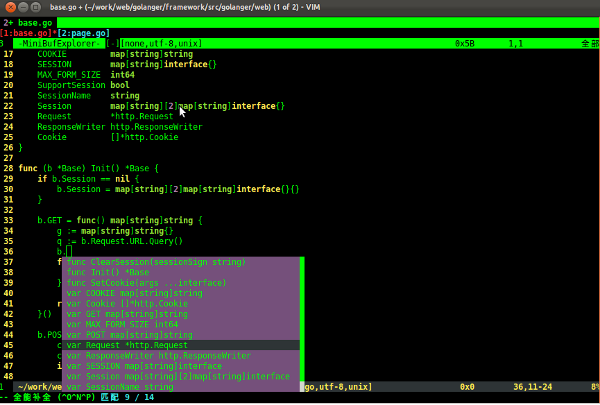
\includegraphics[width=14cm]{1.4.vim.png}
   \label{図1.9}
   \caption{VIMエディタのGoの自動補完画面}
\end{figure}


\begin{enumerate}
\item vimハイライト表示の設定
  \begin{lstlisting}[numbers=none]
cp -r $GOROOT/misc/vim/* ~/.vim/
  \end{lstlisting}
\item ~/.vimrcファイルで文法のハイライト表示を追加します
  \begin{lstlisting}[numbers=none]
filetype plugin indent on
syntax on
  \end{lstlisting}
\item Gocodeをインストールします
  \begin{lstlisting}[numbers=none]
go get -u github.com/nsf/gocode
  \end{lstlisting}
  gocodeはデフォルトで\texttt{\$GOPATH\//bin}の下にインストールされています。
\item Gocodeを設定します。
  \begin{lstlisting}[numbers=none]
~ cd $GOPATH/src/github.com/nsf/gocode/vim
~ ./update.bash
~ gocode set propose-builtins true
propose-builtins true
~ gocode set lib-path "/home/border/gocode/pkg/linux_amd64"
lib-path "/home/border/gocode/pkg/linux_amd64"
~ gocode set
propose-builtins true
lib-path "/home/border/gocode/pkg/linux_amd64"
  \end{lstlisting}
  \begin{quote}
    gocode setの2つのパラメータの意味を説明します:

    propose-builtins:はGoのビルトイン関数を補完するかです。タイプは定数です。デフォルトはfalseで、表示しません。

    lib-path:デフォルトで、gocodeは\$GOPATH\//pkg\//\$GOOS\_\$GOARCHと\$GOROOT\//pkg\//\$GOOS\_\$GOARCHディレクトリのパッケージを検索するだけです。当然この設定には私達の外側のlibを検索できるようパスを設定することができます。
  \end{quote}
\item おめでとうございます。インストール完了です。あなたは今から\texttt{:e main.go}でGoで開発する面白さを体験することができます。
\end{enumerate}


より多くのVIMの設定は、リンク(http:\//\//monnand.me\//p\//vim-golang-environment\//zhCN\//)をご参照ください。

\subsubsection{Emacs}
Emacsは伝説の神器です。彼女はエディタであるだけでなく、統合環境でもあります。または開発環境の集大成と呼んでもよいかもしれません。これらの機能はユーザの身を万能のオペレーティングシステムに置きます。

\begin{figure}[H]
  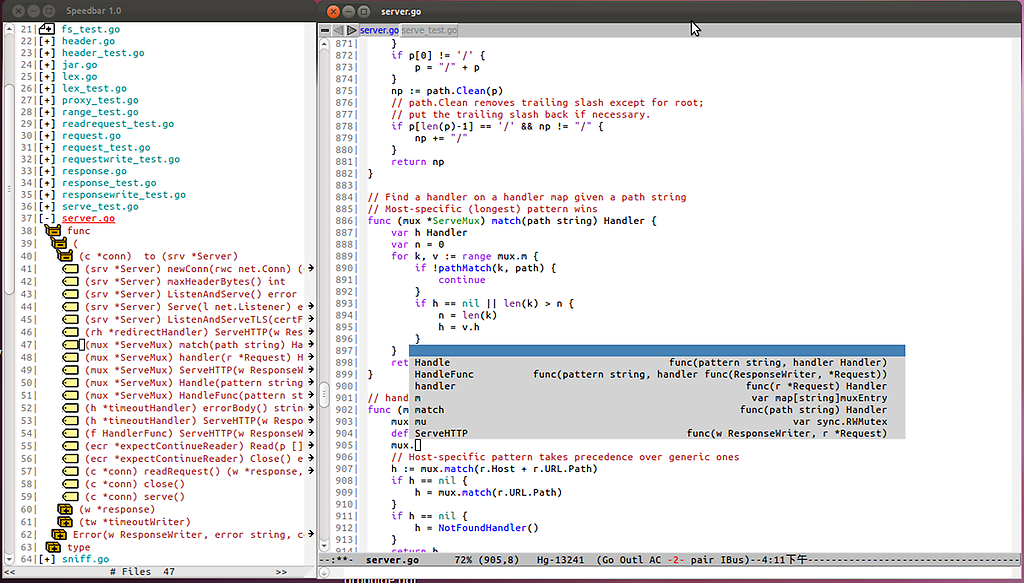
\includegraphics[width=14cm]{1.4.emacs.png}
   \label{図1.10}
   \caption{EmacsでGoを編集するメイン画面}
\end{figure}


\begin{enumerate}
\item Emacsのハイライト表示設定
\begin{lstlisting}[numbers=none]
cp $GOROOT/misc/emacs/* ~/.emacs.d/
\end{lstlisting}
\item Gocodeをインストール
\begin{lstlisting}[numbers=none]
go get -u github.com/nsf/gocode
gocodeはデフォルトで`$GOBIN`の下にインストールされます。
\end{lstlisting}
\item Gocodeを設定
\begin{lstlisting}[numbers=none]
 ~ cd $GOPATH/src/github.com/nsf/gocode/emacs
 ~ cp go-autocomplete.el ~/.emacs.d/
 ~ gocode set propose-builtins true
 propose-builtins true
 ~ gocode set lib-path "/home/border/gocode/pkg/linux_amd64"
                        // あなたのパスに置き換えてください。
 lib-path "/home/border/gocode/pkg/linux_amd64"
 ~ gocode set
 propose-builtins true
 lib-path "/home/border/gocode/pkg/linux_amd64"
\end{lstlisting}
\item Auto Completionをインストールする必要があります。\\ AutoCompleteをダウンロードして解凍します。\\ ~ make install DIR=\$HOME\//.emacs.d\//auto-complete\\ ~\//.emacsファイルを設定します。
\begin{lstlisting}[numbers=none]
;;auto-complete
(require 'auto-complete-config)
(add-to-list 'ac-dictionary-directories
  "~/.emacs.d/auto-complete/ac-dict")
(ac-config-default)
(local-set-key (kbd "M-/") 'semantic-complete-analyze-inline)
(local-set-key "." 'semantic-complete-self-insert)
(local-set-key ">" 'semantic-complete-self-insert)
\end{lstlisting}
詳細情報はこちらを参考にしてください:http://www.emacswiki.org/emacs/AutoComplete
\item .emacsを設定します。
\begin{lstlisting}[numbers=none]
 ;; golang mode
 (require 'go-mode-load)
 (require 'go-autocomplete)
 ;; speedbar
 ;; (speedbar 1)
 (speedbar-add-supported-extension ".go")
 (add-hook
 'go-mode-hook
 '(lambda ()
     ;; gocode
     (auto-complete-mode 1)
     (setq ac-sources '(ac-source-go))
     ;; Imenu & Speedbar
     (setq imenu-generic-expression
         '(("type" "^type *\\([^ \t\n\r\f]*\\)" 1)
         ("func" "^func *\\(.*\\) {" 1)))
     (imenu-add-to-menubar "Index")
     ;; Outline mode
     (make-local-variable 'outline-regexp)
     (setq outline-regexp
       "//\\.\\|//[^\r\n\f][^\r\n\f]\\|pack\\|func\\|impo\\|cons\\|var.\\|type\\|\t\t*....")
     (outline-minor-mode 1)
     (local-set-key "\M-a" 'outline-previous-visible-heading)
     (local-set-key "\M-e" 'outline-next-visible-heading)
     ;; Menu bar
     (require 'easymenu)
     (defconst go-hooked-menu
         '("Go tools"
         ["Go run buffer" go t]
         ["Go reformat buffer" go-fmt-buffer t]
         ["Go check buffer" go-fix-buffer t]))
     (easy-menu-define
         go-added-menu
         (current-local-map)
         "Go tools"
         go-hooked-menu)

     ;; Other
     (setq show-trailing-whitespace t)
     ))
 ;; helper function
 (defun go ()
     "run current buffer"
     (interactive)
     (compile (concat "go run " (buffer-file-name))))

 ;; helper function
 (defun go-fmt-buffer ()
     "run gofmt on current buffer"
     (interactive)
     (if buffer-read-only
     (progn
         (ding)
         (message "Buffer is read only"))
     (let ((p (line-number-at-pos))
     (filename (buffer-file-name))
     (old-max-mini-window-height max-mini-window-height))
         (show-all)
         (if (get-buffer "*Go Reformat Errors*")
     (progn
         (delete-windows-on "*Go Reformat Errors*")
         (kill-buffer "*Go Reformat Errors*")))
         (setq max-mini-window-height 1)
         (if (= 0 (shell-command-on-region
                     (point-min) (point-max)
         "gofmt" "*Go Reformat Output*" nil "*Go Reformat Errors*" t))
     (progn
         (erase-buffer)
         (insert-buffer-substring "*Go Reformat Output*")
         (goto-char (point-min))
         (forward-line (1- p)))
     (with-current-buffer "*Go Reformat Errors*"
     (progn
         (goto-char (point-min))
         (while (re-search-forward "<standard input>" nil t)
         (replace-match filename))
         (goto-char (point-min))
         (compilation-mode))))
         (setq max-mini-window-height old-max-mini-window-height)
         (delete-windows-on "*Go Reformat Output*")
         (kill-buffer "*Go Reformat Output*"))))
 ;; helper function
 (defun go-fix-buffer ()
     "run gofix on current buffer"
     (interactive)
     (show-all)
     (shell-command-on-region (point-min) (point-max)
         "go tool fix -diff"))
\end{lstlisting}
\item おめでとうございます。今からあなたはこの神器を使ってGo開発の楽しみを体験できます。デフォルトのspeedbarは閉じています。もし開く場合は ;; (speedbar 1) の前のコメントを取り去るか、M-x speedbarを手動で起動してください。
\end{enumerate}

\subsubsection{Eclipse}
Eclipseも非常によく使われる開発ツールです。以下ではEclipseを使ってどのようにGoプログラムを編集するかご紹介します。

\begin{figure}[H]
  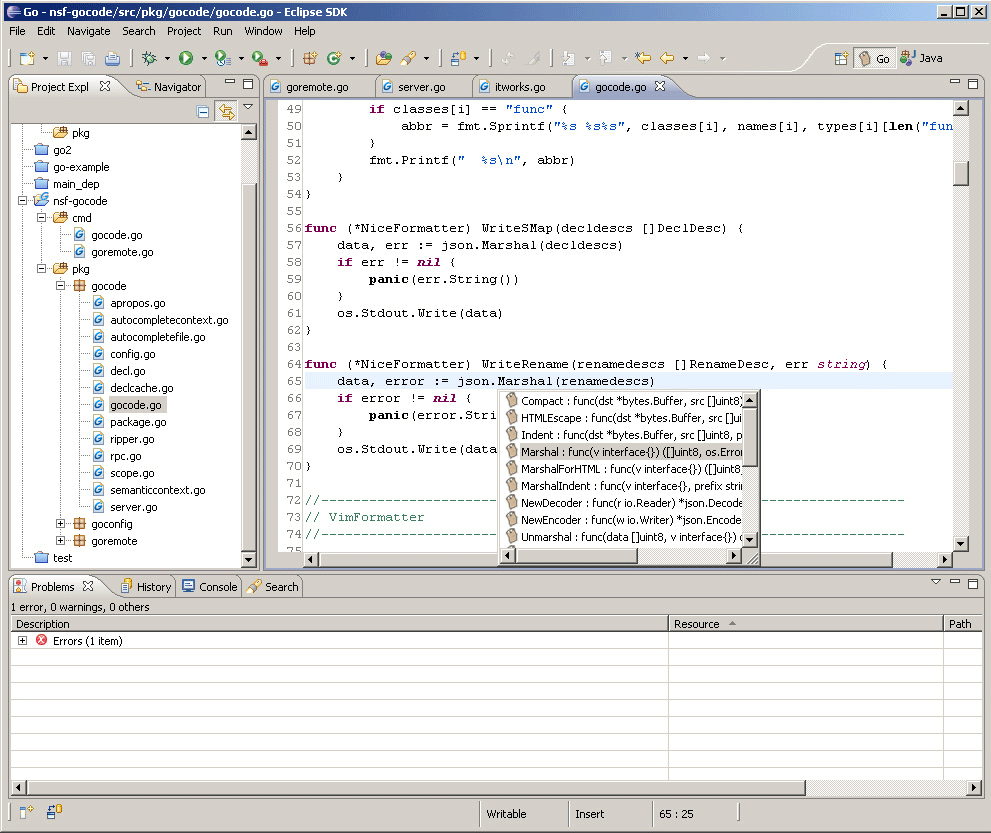
\includegraphics[width=14cm]{1.4.eclipse1.png}
   \label{図1.11}
   \caption{EclipseでのGo編集のメイン画面}
\end{figure}

\begin{enumerate}
\item まずEclipseをダウンロードしてインストールします。
\item goclipseプラグインをダウンロードします。\\ http:\//\//code.google.com\//p\//goclipse\//wiki\//InstallationInstructions
\item gocodeをダウンロードして、goのコード補完を表示させます。
\begin{lstlisting}[numbers=none]
 gocodeのgithubアドレス:
 https://github.com/nsf/gocode
 windowsではgitをインストールする必要があります。通常は
 [msysgit](https://code.google.com/p/msysgit/)を使います。
 cmdでインストールを行います:
 go get -u github.com/nsf/gocode
 以下のコードをダウンロードし、直接go buildでコンパイルしても
 かまいません。
 この場合はgocode.exeが生成されます。
\end{lstlisting}
\item MinGWをダウンロードして要求に従いインストールしてください。
\item プラグイン設定\\ Windows-$>$Reference-$>$Go
  \begin{enumerate}
  \item Goのコンパイラを設定します。
\begin{figure}[H]
  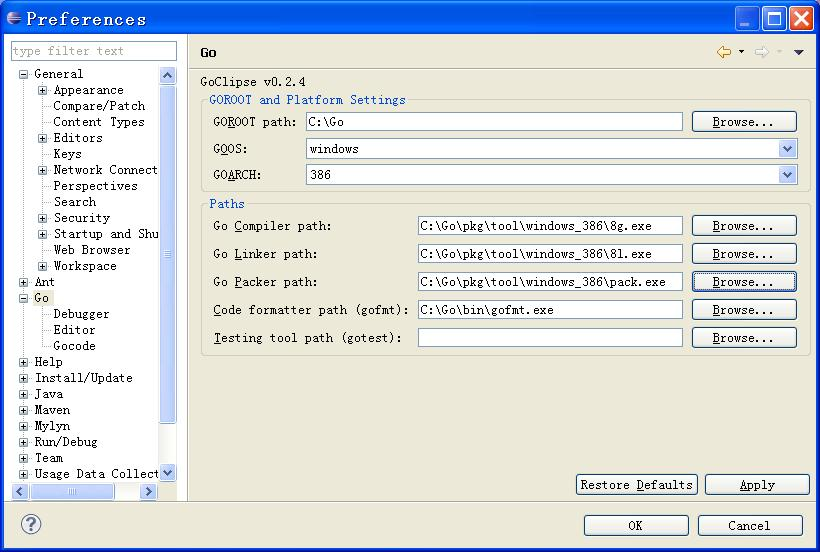
\includegraphics[width=14cm]{1.4.eclipse2.png}
   \label{図1.12}
   \caption{Goの基本情報を設定します。}
\end{figure}
  \item Gocodeを設定します(オプション、コード補完)、Gocodeのパスは事前に生成したgocode.exeファイルを設定します。
\begin{figure}[H]
  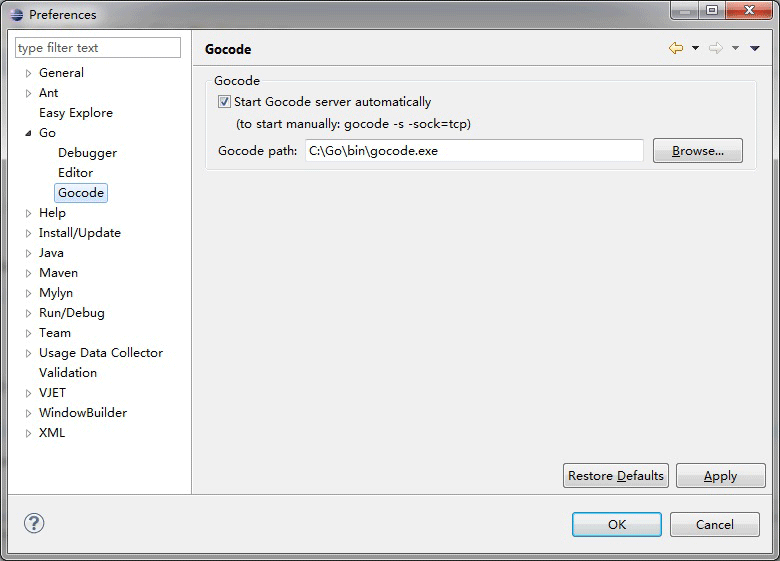
\includegraphics[width=14cm]{1.4.eclipse3.png}
   \label{図1.13}
   \caption{gocode情報を設定します。}
\end{figure}
  \item GDBを設定します(オプション、テスト用)、GDBのパスはMingGWのインストールディレクトリ下のgdb.exeファイルを設定します。
\begin{figure}[H]
  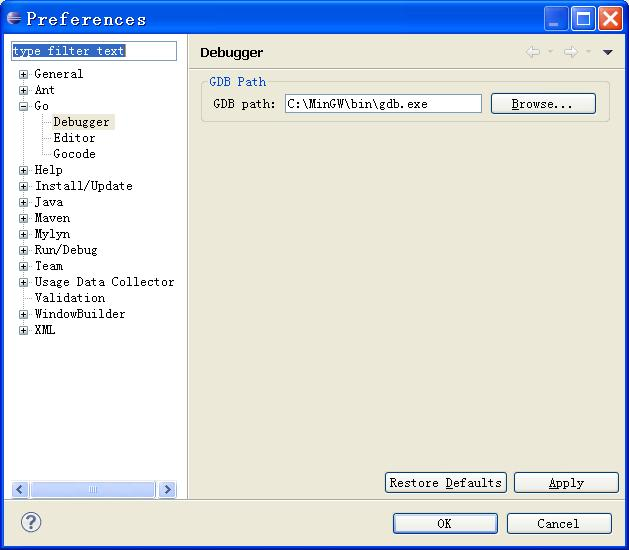
\includegraphics[width=14cm]{1.4.eclipse4.png}
   \label{図1.14}
   \caption{GDB情報の設定}
\end{figure}
  \end{enumerate}
\item テストが成功するか\\ goプロジェクトを一つ新規作成して、hello.goを作成します:
\begin{figure}[H]
   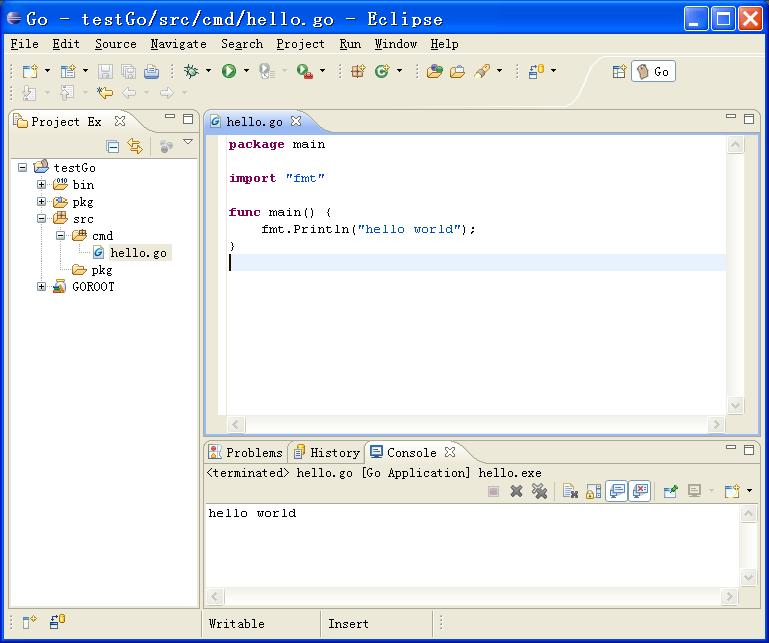
\includegraphics[width=14cm]{1.4.eclipse5.png}
   \label{図1
     .15}
   \caption{プロジェクトの新規作成とファイルの編集}
\end{figure}
\item テストの実行(consoleでコマンドを入力する必要があります):
\begin{figure}[H]
  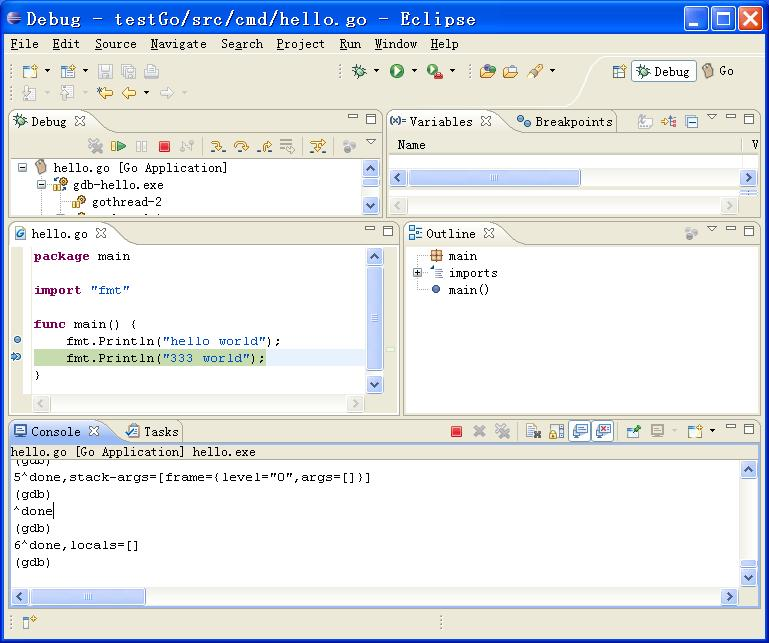
\includegraphics[width=14cm]{1.4.eclipse6.png}
   \label{図1.16}
   \caption{Goプログラムのテスト}
\end{figure}
\end{enumerate}

\subsubsection{IntelliJ IDEA}
Javaに親しい読者はideaに詳しいことでしょう。ideaはプラグインを通してgo言語のシンタックスハイライト、コード補完およびリビルドをサポートしています。

\begin{enumerate}
  \item ideaを先にダウンロードします。ideaはマルチプラットフォームをサポートしています:win,mac,linux、もしお金があれば正式版を購入します、もし無ければ、コミュニティの無料版を使ってください。Go言語を開発するだけであれば無料版で十分事足ります。
    \begin{figure}[H]
      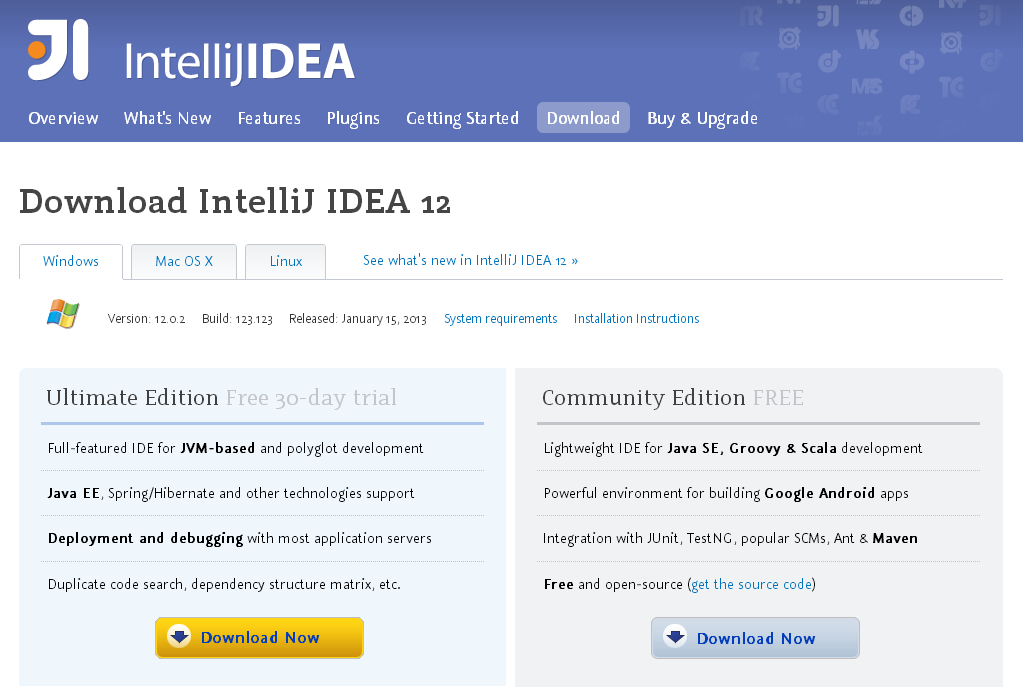
\includegraphics[width=14cm]{1.4.idea1.png}
    \end{figure}
  \item Goプラグインをインストールし、FileメニューのSettingをクリックします。Pluginsを探したら、Browser repoボタンをクリックします。中国国内のユーザはおそらくエラーが出るかもしれませんが、自分で解決してくれよな。
    \begin{figure}[H]
      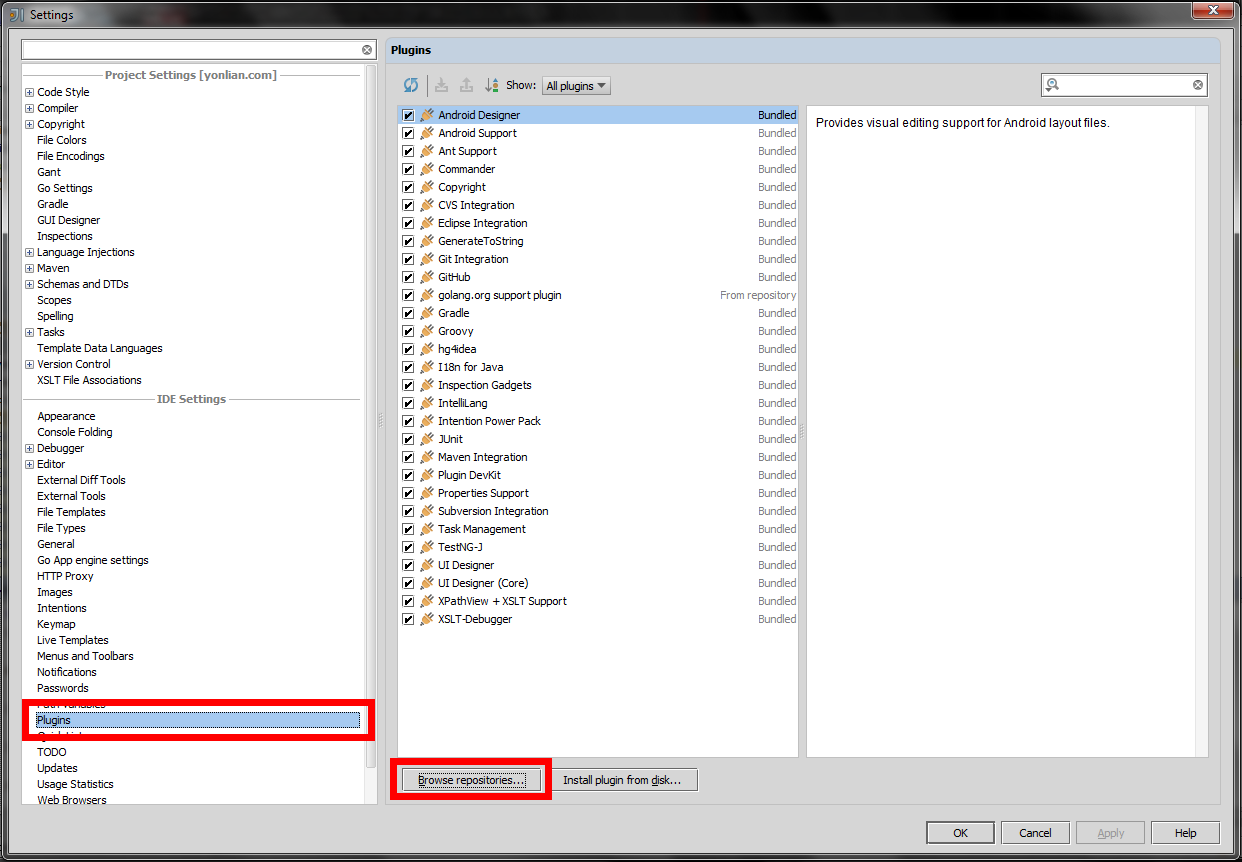
\includegraphics[width=14cm]{1.4.idea3.png}
    \end{figure}
  \item この時いくつものプラグインが見つかります。Golangを検索して、download and installをダブルクリックしてください。golangの行末にDownloadedの表示が現れるのを待って、OKをクリックします。
    \begin{figure}[H]
      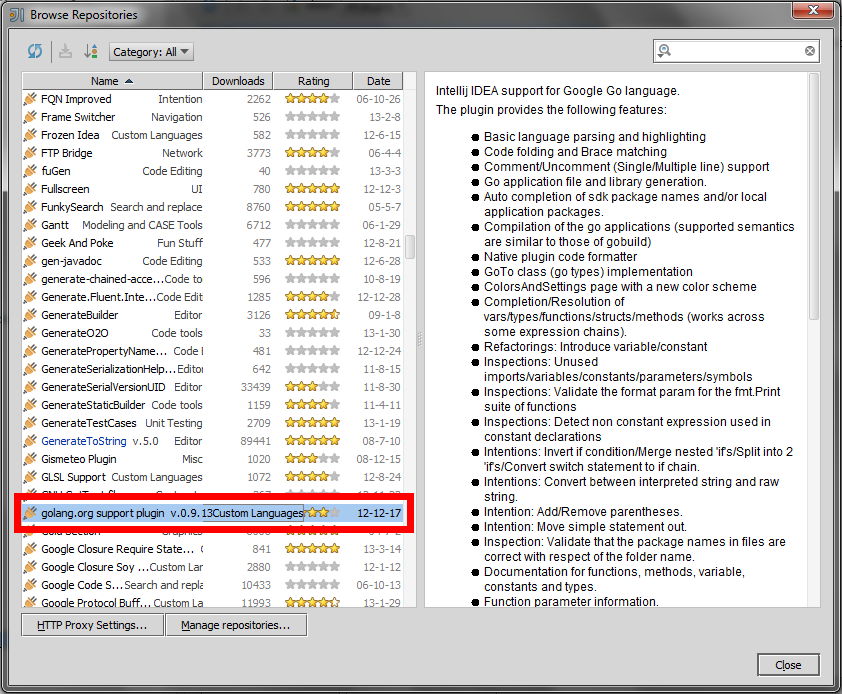
\includegraphics[width=14cm]{1.4.idea4.png}
    \end{figure}
    その後Applyをクリックすると、IDEが再起動を要求します。
  \item 再起動が完了し、新規プロジェクトを作成すると、golangプロジェクトが作成可能であることがお分かりいただけるかとおもいます:
    \begin{figure}[H]
      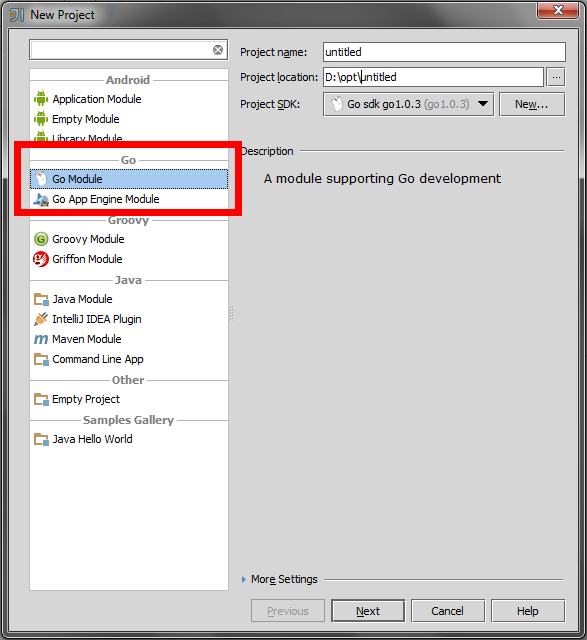
\includegraphics[width=14cm]{1.4.idea5.png}
    \end{figure}
    次に、go sdkの場所を入力するよう促されるかもしれません。普段はいつもC:\textbackslash Goにインストールされています。Linuxとmacは自分のインストールディレクトリの設定にしたがって、ディレクトリを選択すれば大丈夫です。
\end{enumerate}


\subsection{まとめ}
この章では主にどのようにしてGoをインストールするかについてご紹介しました。Goは3つの種類のインストール方法があります:ソースコードインストール、標準パッケージインストール、サードパーティツールによるインストールです。インストール後開発環境を整え、ローカルの\texttt{\$GOPATH}を設定します。\texttt{\$GOPATH}設定を通じて読者はプロジェクトを作成することができます。次にどのようにプロジェクトをコンパイルするのか説明しました。アプリケーションのインストールといった問題はたくさんのGoコマンドを使用する必要があります。そのため、Goで日常的に用いられるコマンドツールについてもご説明しました。コンパイル、インストール、整形、テストなどのコマンドです。最後にGoの開発ツールについてご紹介しました。現在多くのGoの開発ツールには:LiteIDE、sublime、VIM、Emacs、Eclipse、Ideaといったツールがあります。読者は自分が一番慣れ親しんだツールを設定することができます。便利なツールで素早くGoアプリケーションを開発できるよう願っています。



\section{Go言語の基礎}
GoはCに似たコンパイラ型言語です。ですが、このコンパイル速度は非常に速く、この言語のキーワードもたったの25個です。英文よりも少し少なく勉強するにはかなり簡単です。まずはこれらのキーワードがどのようなものか見てみることにしましょう:

\begin{lstlisting}[numbers=none]
break    default      func    interface    select
case     defer        go      map          struct
chan     else         goto    package      switch
const    fallthrough  if      range        type
continue for          import  return       var
\end{lstlisting}

この章では、この言語の基礎勉強にあなたを連れていきます。各章の紹介を通じて、Goの世界がどれほどまでに簡潔で絶妙にデザインされているかお分かりいただけるはずです。Goを書くことはとても楽しいことです。後から振り返ると、この25個のキーワードがどれだけフレンドリーか理解するはずです。


\subsection{こんにちは、Go}
\section{Basics}

出発点は言語の全ての基本を学ぶことです。

変数の宣言方法や関数の呼び出し方、次のレッスンに移る前に知っておくべき全てのこと。

\subsection{Packages}

Goのプログラムは、パッケージ( package )で構成されます。

プログラムは \texttt{main} パッケージから開始されます。

このプログラムでは \texttt{"fmt"} と \texttt{"math/rand"} パッケージをインポート( import )しています。

規約で、パッケージ名はインポートパスの最後の要素と同じ名前になります。
例えば、インポートパスが \texttt{"math/rand"} のパッケージは、
\texttt{package rand} ステートメントで始まるファイル群で構成します。

\textbf{Note}: ここで実行するプログラムは常に同じ環境で実行されますので、
擬似乱数を返す \texttt{rand.Intn} はいつも同じ数を返します。

(数を強制的に変える場合は、乱数生成でシードを与える必要があります。
\texttt{rand.Seed}を見てみてください。
playground 上での時間は一定なので他のものをシードとして使う必要があります。)

\lstinputlisting[caption = packages.go]{packages.go}
\lstinputlisting[caption = packages.run,numbers=none]{packages.run}

\subsection{Imports}

このコードでは、括弧でパッケージのインポートをグループ化し、
factoredインポートステートメント( factored import statement )としています。

もちろん、複数のインポートステートメントで書くこともできます:

\begin{lstlisting}[firstnumber=3]
import "fmt"
import "math"
\end{lstlisting}

ですが、先に示したfactoredインポートステートメントの方がより良いスタイルです。

訳注: ここの factored の意味は、「要素化、グループ化、整理済み」ということです。
良い日本語募集中。

\lstinputlisting[caption = imports.go]{imports.go}
\lstinputlisting[caption = imports.run,numbers=none]{imports.run}

\subsection{Exported names}
Goでは、最初の文字が大文字で始まる名前は、
外部のパッケージから参照できるエクスポート(公開)された
名前( exported name )です。 
例えば、 \texttt{Pi} は \texttt{math} パッケージでエクスポートされています。

小文字ではじまる \texttt{pi} や \texttt{hoge} などは
エクスポートされていない名前です。

パッケージをインポートすると、そのパッケージがエクスポートしている名前を
参照することができます。 エクスポートされていない名前(小文字ではじまる名前)は、
外部のパッケージからアクセスすることはできません。

コードを実行し、エラーを確認してみましょう。

エラーを修正するために、 \texttt{math.pi} を \texttt{math.Pi} に書き換え、
もう一度実行してみてください。

\lstinputlisting[caption = exported-names.go]{exported-names.go}
\lstinputlisting[caption = エラーする場合,numbers=none]{exported-names.run1}
\lstinputlisting[caption = 修正した実行イメージ,numbers=none]{exported-names.run}

\subsection{Functions}

関数は、0個以上の引数を取ることができます。

この例では、 \texttt{add} 関数は、 \texttt{int} 型の2つのパラメータを取ります。

変数名の {\large {\textbf{後ろ}}} に型名を書くことに注意してください。

(型をなぜこのように宣言するのか、についての詳細な情報は、 記事「Go's declaration syntax」 を参照してください。)
\lstinputlisting[caption = functions.go]{functions.go}
\lstinputlisting[caption = functions.run,numbers=none]{functions.run}

\subsection{Functions continued}

関数の2つ以上の引数が同じ型である場合には、最後の型を残して省略して記述できます。

この例では、
\begin{lstlisting}[firstnumber=5]
x int, y int
\end{lstlisting}
を

\begin{lstlisting}[firstnumber=5]
x, y int
\end{lstlisting}
へ省略できます。
\lstinputlisting[caption = functions-continued.go]{functions-continued.go}
\lstinputlisting[caption = functions-continued.run,numbers=none]{functions-continued.run}

\subsection{Multiple results}

関数は複数の戻り値を返すことができます。

この \texttt{swap} 関数は2つの string を返します。 とても簡単に交換できますね!
\lstinputlisting[caption = functions.go]{multipul-results.go}
\lstinputlisting[caption = functions.run,numbers=none]{multipul-results.run}

\subsection{Named return values}
Goでの戻り値となる変数に名前をつける( named return value )ことができます。
戻り値に名前をつけると、関数の最初で定義した変数名として扱われます。

この戻り値の名前は、戻り値の意味を示す名前とすることで、関数のドキュメントとして
表現するようにしましょう。

名前をつけた戻り値の変数を使うと、 \texttt{return} ステートメントに何も書かずに
戻すことができます。これを "naked" return と呼びます。

例のコードのように、naked returnステートメントは、短い関数でのみ利用すべきです。
長い関数で使うと読みやすさ( readability )に悪影響があります。
\lstinputlisting[caption = named-results.go]{named-results.go}
\lstinputlisting[caption = named-results.run,numbers=none]{named-results.run}

\subsection{Variables}
\texttt{var} ステートメントは変数( variable )を宣言します。 
関数の引数リストと同様に、複数の変数の最後に型を書くことで、
変数のリストを宣言できます。

\texttt{var} ステートメントはパッケージ、または、関数で利用できます。
例のコードで示します。
\lstinputlisting[caption = variables.go]{variables.go}
\lstinputlisting[caption = variables.run,numbers=none]{variables.run}

\subsection{Variables with initializers}
\texttt{var} 宣言では、変数毎に初期化子( initializer )を与えることができます。

初期化子が与えられている場合、型を省略できます。
その変数は初期化子が持つ型になります。
\lstinputlisting[caption = variables-with-initializers.go]{variables-with-initializers.go}
\lstinputlisting[caption = variables-with-initializers.run,numbers=none]{variables-with-initializers.run}

\subsection{Short variable declarations}
関数の中では、 \texttt{var} 宣言の代わりに、短い \texttt{:=} の代入文を使い、
暗黙的な型宣言ができます。

なお、関数の外では、キーワードではじまる宣言( \texttt{var}, \texttt{func}, など)が必要で、
\texttt{:=} での暗黙的な宣言は利用できません。
\lstinputlisting[caption = short-variable-declarations.go]{short-variable-declarations.go}
\lstinputlisting[caption = short-variable-declarations.run,numbers=none]{short-variable-declarations.run}

\subsection{Basic types}
Go言語の基本型(組み込み型)は次のとおりです:

\begin{lstlisting}[numbers=none]
bool

string

int  int8  int16  int32  int64
uint uint8 uint16 uint32 uint64 uintptr

byte // uint8 の別名

rune // int32 の別名
     // Unicode のコードポイントを表す

float32 float64

complex64 complex128
\end{lstlisting}

(訳注:runeとは古代文字を表す言葉(runes)ですが、
Goでは文字そのものを表すためにruneという言葉を使います。)

例では、いくつかの型の変数を示しています。また、変数宣言は、
インポートステートメントと同様に、まとめて( factored )宣言可能です。

\texttt{int}, \texttt{uint}, \texttt{uintptr} 型は、
32-bitのシステムでは32 bitで、
64-bitのシステムでは64 bitです。 
サイズ、符号なし( unsigned )整数の型を使うための特別な理由がない限り、
整数の変数が必要な場合は \texttt{int} を使うようにしましょう。
\lstinputlisting[caption = basic-types.go]{basic-types.go}
\lstinputlisting[caption = basic-types.run,numbers=none]{basic-types.run}

\subsection{Zero values}
変数に初期値を与えずに宣言すると、ゼロ値( zero value )が与えられます。

ゼロ値は型によって以下のように与えられます:

\begin{description}
    \item 数値型(int,floatなど): \texttt{0}
    \item bool型: \texttt{false}
    \item string型: \texttt{""} (空文字列( empty string ))
\end{description}
\lstinputlisting[caption = zero.go]{zero.go}
\lstinputlisting[caption = zero.run,numbers=none]{zero.run}

\subsection{Type conversions}
{\large 型変換}

変数 \texttt{v} 、型 \texttt{T} があった場合、 \texttt{T(v)} は、
変数 \texttt{v} を \texttt{T} 型へ変換します。

いくつかの変換を見てみましょう:

\begin{lstlisting}[numbers=none]
var i int = 42
var f float64 = float64(i)
var u uint = uint(f)
\end{lstlisting}

よりシンプルに記述できます:

\begin{lstlisting}[numbers=none]
i := 42
f := float64(i)
u := uint(f)
\end{lstlisting}

C言語とは異なり、Goでの型変換は明示的な変換が必要です。
例のコードで、 \texttt{float64} や \texttt{uint} の変換
を削除し、何が起きるのか確認しましょう。
\lstinputlisting[caption = type-conversions.go]{type-conversions.go}
\lstinputlisting[caption = type-conversions.run,numbers=none]{type-conversions.run}
\lstinputlisting[caption = 変換を削除した場合,numbers=none]{type-conversions.run1}

\subsection{Type inference}
明示的な型を指定せずに変数を宣言する場合
( \texttt{:=} や \texttt{var =} のいずれか)、
変数の型は右側の変数から型推論されます。

右側の変数が型を持っている場合、左側の新しい変数は同じ型になります:

\begin{lstlisting}[numbers=none]
var i int
j := i // j is an int
\end{lstlisting}

右側に型を指定しない数値である場合、左側の新しい変数は
右側の定数の精度に基いて \texttt{int}, \texttt{float64},
\texttt{complex128} の型になります:

\begin{lstlisting}[numbers=none]
i := 42           // int
f := 3.142        // float64
g := 0.867 + 0.5i // complex128
\end{lstlisting}

例のコードにある変数 \texttt{v} の初期値を変えて、
型がどのように変化するかを見てみてください。
\lstinputlisting[caption = type-inference.go]{type-inference.go}
\lstinputlisting[caption = type-inference.run,numbers=none]{type-inference.run}

\subsection{Constants}
定数( constant )は、 \texttt{const} キーワードを使って変数と同じように宣言します。

定数は、文字(character)、文字列(string)、boolean、数値(numeric)のみで使えます。

なお、定数は \texttt{:=} を使って宣言できません。
\lstinputlisting[caption = constants.go]{constants.go}
\lstinputlisting[caption = constants.run,numbers=none]{constants.run}

\subsection{Numeric Constants}
数値の定数は、高精度な 値 ( values )です。

型のない定数は、その状況によって必要な型を取ることになります。

例で \texttt{needInt(Big)} も出力してみてください。

( \texttt{int} は最大64-bitの整数を保持できますが、環境によっては精度が低いこともあります)
\lstinputlisting[caption = numeric-constants.go]{numeric-constants.go}
\lstinputlisting[caption = numeric-constants.run,numbers=none]{numeric-constants.run}
\lstinputlisting[caption = needInt(Big) の出力,numbers=none]{numeric-constants.run1}

\subsection{Goの基礎}
この節では変数、定数、Goの内部クラスの定義と、Goプログラムの設計におけるテクニックをご紹介します。

\subsubsection{変数の定義}
Go言語では変数は数多くの方法で定義されます。

\texttt{var}キーワードを使用することはGoの最も基本的な変数の定義方法です。C言語と異なり、Goでは変数の型を変数の後に置きます。


\begin{lstlisting}[numbers=none]
//"variableName"という名前で定義します。型は"type"です。
var variableName type
\end{lstlisting}

複数の変数を定義します。

\begin{lstlisting}[numbers=none]
//すべて"type"型の3つの変数を定義します。
var vname1, vname2, vname3 type
\end{lstlisting}

変数を定義し、初期化します。

\begin{lstlisting}[numbers=none]
//"variableName"の変数を"value"で初期化します。型は"type"です。
var variableName type = value
\end{lstlisting}

複数の変数を同時に初期化します。

\begin{lstlisting}[numbers=none]
/*
  すべてが"type"型となる変数をそれぞれ定義し、個別に初期化を行います。
  vname1はv1,vname2はv2,vname3はv3
*/
var vname1, vname2, vname3 type= v1, v2, v3
\end{lstlisting}

あなたは上述の定義が面倒だと思いますか?大丈夫、Go言語の設計者もわかっています。少し簡単に書くこともできます。直接型の宣言を無視することができるので、上のコードはこのようにも書けます:

\begin{lstlisting}[numbers=none]
/*
   3つの変数を定義し、それぞれ個別に初期化する。
   vname1はv1,vname2はv2,vname3はv3
   このあとGoは代入される値の肩に従ってそれぞれ初期化を行います。
*/
var vname1, vname2, vname3 = v1, v2, v3
\end{lstlisting}

これでもまだ面倒ですか?ええ、私もそう思います。更に簡単にしてみましょう。

\begin{lstlisting}[numbers=none]
/*
   3つの変数を定義し、それぞれ個別に初期化します。
   vname1はv1,vname2はv2,vname3はv3
   コンパイラは初期化する値に従って自動的にふさわしい型を導き出します。
*/
vname1, vname2, vname3 := v1, v2, v3
\end{lstlisting}

これなら非常に簡潔になったでしょう?\texttt{:=}の記号は\texttt{var}と\texttt{type}に直接取って代わるものです。これらの形式を短縮宣言と呼びます。ただしこれにはひとつ制限があります。これらは関数の内部でしか使用できません。関数の外で使用するとコンパイルが通らなくなります。そのため、一般的には\texttt{var}方式でグローバル変数が定義されます。

\texttt{\_}(アンダースコア)は特別な変数名です。どのような値もすべて捨てられてしまいます。この例では\texttt{35}という値を\texttt{b}に与えますが、同時に\texttt{34}は失われてしまいます。

\begin{lstlisting}[numbers=none]
_, b := 34, 35
\end{lstlisting}

Goはすでに宣言されている未使用の変数をコンパイル時にエラーとして出力します。例えば下のコードはエラーを一つ生成します。\texttt{i}は宣言されましたが使用されていません。

\begin{lstlisting}[numbers=none]
package main

func main() {
    var i int
}
\end{lstlisting}





\subsubsection{定数}
いわゆる定数というのは、プログラムがコンパイルされる段階で値が決定されます。そのため、プログラムが実行される時には値の変更は許されません。定数には数値、bool値または文字列等の型を定義することができます。

この文法は以下の通りです:

\begin{lstlisting}[numbers=none]
const constantName = value
//もし必要であれば、定数の型を明示することもできます:
const Pi float32 = 3.1415926
\end{lstlisting}

ここでは定数の宣言の例を示します:

\begin{lstlisting}[numbers=none]
const Pi = 3.1415926
const i = 10000
const MaxThread = 10
const prefix = "astaxie_"
\end{lstlisting}

Go の定数は一般的なプログラミング言語と異なり、かなり多くの小数点以下の桁を指定することができます(たとえば200桁など)、 float32に自動的な32bitへの短縮を指定したり、float64に自動的な64bitへの短縮を指定するにはリンク(http:\//\//golang.org\//ref\//spec\#Constants)をご参照ください。

\subsubsection{ビルトイン基本型}
\paragraph{Boolean}
Goではbool値の型は\texttt{bool}です。値は\texttt{true}もしくは\texttt{false}です。デフォルト値は\texttt{false}です。

\begin{lstlisting}[numbers=none]
// コード例
var isActive bool  // グローバル変数の宣言
var enabled, disabled = true, false  // 型を省略した宣言
func test() {
    var available bool  // 通常の宣言
    valid := false      // 短縮宣言
    available = true    // 代入操作
}
\end{lstlisting}

\paragraph{数値型}
整数型には符号付きと符号無しの2つがあります。Goはまた\texttt{int}と\texttt{uint}をサポートしています。この2つの型の長さは同じですが、実際の長さは異なるコンパイラによって決定されます。Goでは直接bit数を指定できる型もあります:\texttt{rune}, \texttt{int8}, \texttt{int16}, \texttt{int32}, \texttt{int64}と\texttt{byte}, \texttt{uint8}, \texttt{uint16}, \texttt{uint32}, \texttt{uint64}です。この中で\texttt{rune}は\texttt{int32}のエイリアスです。\texttt{byte}は\texttt{uint8}のエイリアスです。

\begin{quote}
注意しなければならないのは、これらの型の変数間は相互に代入または操作を行うことができないということです。コンパイル時にコンパイラはエラーを発生させます。

下のコードはエラーが発生します。:invalid operation: a + b (mismatched types int8 and int32)
\begin{lstlisting}[numbers=none]
    var a int8
    var b int32
    c:=a + b
\end{lstlisting}
また、intの長さは32bitですが、intとint32もお互いに利用することはできません。
\end{quote}

浮動小数点の型には\texttt{float32}と\texttt{float64}の二種類があります(\texttt{float}型はありません。)。デフォルトは\texttt{float64}です。

これで全てですか?No! Goは複素数もサポートしています。このデフォルト型は\texttt{complex128}(64bit実数+64bit虚数)です。もしもう少し小さいのが必要であれば、\texttt{complex64}(32bit実数+32bit虚数)もあります。複素数の形式は\texttt{RE + IMi}です。この中で\texttt{RE}が実数部分、\texttt{IM}が虚数部分になります。最後の\texttt{i}は虚数単位です。以下に複素数の使用例を示します:

\begin{lstlisting}[numbers=none]
var c complex64 = 5+5i
//output: (5+5i)
fmt.Printf("Value is: %v", c)
\end{lstlisting}

\paragraph{文字列}
前の章で述べた通り、Goの文字列はすべて\texttt{UTF-8}コードが採用されています。文字列は一対のダブルクォーテーション(\texttt{""})またはバッククォート(\texttt{` `} )で括られることで定義されます。この型は\texttt{string}です。

\begin{lstlisting}[numbers=none]
//コード例
var frenchHello string  // 文字列変数の宣言の一般的な方法
var emptyString string = ""
// 文字列変数を一つ宣言し、空文字列で初期化する。
func test() {
    no, yes, maybe := "no", "yes", "maybe"
    // 短縮宣言、同時に複数の変数を宣言
    japaneseHello := "Konichiwa"  // 同上
    frenchHello = "Bonjour"  // 通常の代入
}
\end{lstlisting}

Goの文字列は変更することができません。例えば下のコードはコンパイル時にエラーが発生します。:cannot assign to s[0]

\begin{lstlisting}[numbers=none]
var s string = "hello"
s[0] = 'c'
\end{lstlisting}

ただし、本当に変更したくなったらどうしましょうか?ここでは以下のコードで実現します:

\begin{lstlisting}[numbers=none]
s := "hello"
c := []byte(s)  // 文字列 s を []byte 型にキャスト
c[0] = 'c'
s2 := string(c)  // もう一度 string 型にキャストし直す
fmt.Printf("%s\n", s2)
\end{lstlisting}

Goでは+演算子を使って文字列を連結することができます:

\begin{lstlisting}[numbers=none]
s := "hello,"
m := " world"
a := s + m
fmt.Printf("%s\n", a)
\end{lstlisting}

文字列の修正もこのように書けます:

\begin{lstlisting}[numbers=none]
s := "hello"
s = "c" + s[1:] // 文字列を変更することはできませんが
                // スライスは行えます。
fmt.Printf("%s\n", s)
\end{lstlisting}

もし複数行の文字列を宣言したくなったらどうしましょうか?この場合\texttt{` }で宣言することができます:

\begin{lstlisting}[numbers=none]
m := `hello
    world`
\end{lstlisting}

\texttt{`} で括られた文字列はRaw文字列です。すなわち、文字列はコード内の形式がそのままプリント時の形式になります。文字列の変更はありません。改行はそのまま出力されます。例えばこの例では以下のように出力されます:

\begin{lstlisting}[numbers=none]
hello
    world
\end{lstlisting}


\paragraph{エラー型}
Goにはビルトインの\texttt{error}型があります。専らエラー情報の処理に使用されます。Goの\texttt{package}の中にはエラー処理を行う\texttt{errors}というパッケージがあります。


\begin{lstlisting}[numbers=none]
err := errors.New("emit macho dwarf: elf header corrupted")
if err != nil {
    fmt.Print(err)
}
\end{lstlisting}

\subsubsection{Goデータの低レイヤの保存}
下の図はRuss Cox Blogの中の一文で紹介されているGoデータ構造の文章です。これらの基本型は低レイヤでメモリを分配し、対応する値を保存していることが見て取れるとおもいます。

\begin{figure}[H]
  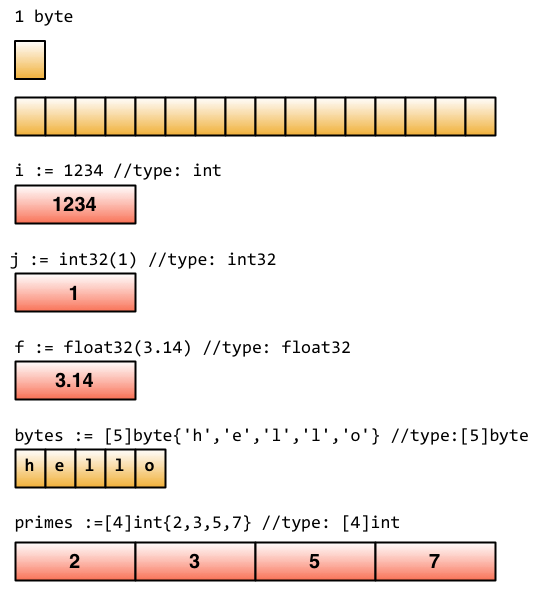
\includegraphics[width=14cm]{2.2.basic.png}
   \label{図2.1}
   \caption{Goデータ形式の保存}
\end{figure}

\subsubsection{テクニック}
\paragraph{グループ化による宣言}
Go言語では、複数の定数・変数を宣言する場合、または複数のパッケージをインポートする場合、グループ化による方法で宣言することができます。

例えば以下のコード:

\begin{lstlisting}[numbers=none]
import "fmt"
import "os"

const i = 100
const pi = 3.1415
const prefix = "Go_"

var i int
var pi float32
var prefix string
\end{lstlisting}

グループ化によって以下のような形式になります:

\begin{lstlisting}[numbers=none]
import(
    "fmt"
    "os"
)

const(
    i = 100
    pi = 3.1415
    prefix = "Go_"
)

var(
    i int
    pi float32
    prefix string
)
\end{lstlisting}



\paragraph{iota列挙型}
Goでは\texttt{iota}というキーワードがあります。このキーワードは\texttt{enum}を宣言する際に使用されます。このデフォルト値は0からはじまり、順次1が追加されます:



\begin{lstlisting}[numbers=none]
const(
    x = iota  // x == 0
    y = iota  // y == 1
    z = iota  // z == 2
    w  // 定数の宣言で値を省略した場合、デフォルト値は
       // 前の値と同じになります。ここではw = iotaと
       // 宣言していることと同じになりますので、
       // w == 3となります。実は上のyとzでも
       // この"= iota"は省略することができます。
)

 const v = iota // constキーワードが出現する度に、
          // iotaは置き直されます。ここではv == 0です。

const ( 
  e, f, g = iota, iota, iota //e=0,f=0,g=0 iotaの同一行は同じです
  )
\end{lstlisting}

\begin{quote}
他の値や\texttt{iota}に設定されているものを除いて、各\texttt{const}グループのはじめの定数はデフォルトで0となります。二番目以降の定数は前の定数の値がデフォルト値となります。もし前の定数の値が\texttt{iota}であれば、直後の値も\texttt{iota}になります。
\end{quote}


\subsubsection{Goプログラムのデザインルール}
Goがこのように簡潔なのは、それがいくつかのデフォルトの行為を持っているからです:

\begin{itemize}
  \item 大文字で始まる変数はエクスポート可能です。つまり、他のパッケージから読むことができる、パブリックな変数だということです。対して小文字で始まる変数はエクスポートできません。これはプライベート変数です。
  \item 大文字で始まる関数も同じです。\texttt{class}の中で\texttt{public}キーワードによってパブリック関数となっているのと同じです。対して小文字で始まる関数は\texttt{private}キーワードのプライベート関数です。
\end{itemize}

\paragraph{array}
\texttt{array}は配列です。この定義は以下のようになります:

\begin{lstlisting}[numbers=none]
var arr [n]type
\end{lstlisting}

\texttt{[n]type}の中で、\texttt{n}は配列の長さを表しています。\texttt{type}は保存する要素の型を示しています。配列に対する操作は他の言語とよく似ていて、どれも\texttt{[]}を通して値の取得および代入を行います。

\begin{lstlisting}[numbers=none]
var arr [10]int  // int型の配列を宣言します。
arr[0] = 42      // 配列のインデックスは0からはじまります。
arr[1] = 13      // 代入操作
fmt.Printf("The first element is %d\n", arr[0])
                 // データを取得して、42を返します。
fmt.Printf("The last element is %d\n", arr[9])
                 // 値が代入されていない最後の要素を返します。
                 // デフォルトでは0が返ります。
\end{lstlisting}

長さも配列の一部ですので、\texttt{[3]int}と\texttt{[4]int}は異なる型になります。配列も長さを変えることはできません。配列間の代入は値渡しです。つまり、一つの配列が関数の引数となった場合、渡されるのは実はこの配列のコピーであり、ポインタではありません。もしポインタを使いたい場合は、この後にご紹介する\texttt{slice}型をご利用ください。

配列はもうひとつの\texttt{:=}で宣言することができます。

\begin{lstlisting}[numbers=none]
a := [3]int{1, 2, 3} // 長さが3のintの配列を宣言します。

b := [10]int{1, 2, 3} // 長さが10のint配列を宣言します。
                      // この中で3つの要素の初期値は1、2、3で、
                      // そのほかのデフォルトは0です。

c := [...]int{4, 5, 6} // 長さを`...`で省略することも
                      // できます。Goは自動で要素数から長さを
                      // 計算します。
\end{lstlisting}

もしあなたが「配列に配列を込めたい場合は実現できますか?」と問うならば、当然ですとも、とお応えしましょう。Goはネストした配列をサポートしています。例えば下のコードでは二次元配列を宣言しています:


\begin{lstlisting}[numbers=none]
  // 二次元配列を一つ宣言します。この配列は
  // 2つの配列を要素としており、各配列には4つ
  // のint型の要素が含まれます。
doubleArray := [2][4]int{[4]int{1, 2, 3, 4},
                           [4]int{5, 6, 7, 8}}

    // 上の宣言は簡略化できます。直接内部の型を省略しています。
easyArray := [2][4]int{{1, 2, 3, 4}, {5, 6, 7, 8}}
\end{lstlisting}

配列の状態は以下のとおりです:

\begin{figure}[H]
  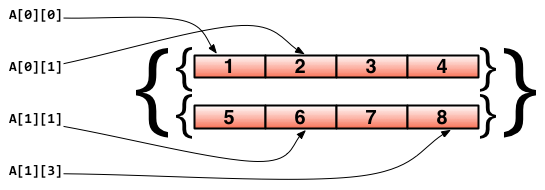
\includegraphics[width=14cm]{2.2.array.png}
   \label{図2.2}
   \caption{多次元配列のマッピング関係}
\end{figure}


\paragraph{slice}
多くのアプリケーションでは、配列はあまりわたしたちの要求を満たしてはくれません。配列を初期化する場合、どれぐらいの大きさの配列が必要かわからないからです。そのため、"動的な配列"が必要となります。Goではこのようなデータ構造を\texttt{slice}と呼びます。

\texttt{slice}は本当の意味での動的な配列ではありません。これは単なる参照型です。\texttt{slice}は常に低レイヤの\texttt{array}を指しています。\texttt{slice}の宣言も\texttt{array}と同様に長さを指定する必要はありません。

\begin{lstlisting}[numbers=none]
// arrayの宣言と同じですが、長さは必要ありません。
var fslice []int
\end{lstlisting}

次に\texttt{slice}を宣言すると同時にデータを初期化します:

\begin{lstlisting}[numbers=none]
slice := []byte {'a', 'b', 'c', 'd'}
\end{lstlisting}

\texttt{slice}はひとつの配列またはすでに存在する\texttt{slice}の中から宣言することができます。\texttt{slice}は\texttt{array[i:j]}で取得することができます。この中で\texttt{i}は配列の開始位置です。\texttt{j}は終了位置です。ただし\texttt{array[j]}は含みません。長さは\texttt{j-i}となります。

\begin{lstlisting}[numbers=none]
// 10個の要素を宣言します。要素の型はbyteの配列です。
var ar = [10]byte {'a', 'b', 'c', 'd', 'e',
                   'f', 'g', 'h', 'i', 'j'}

// byteを含む2つのsliceを宣言します
var a, b []byte

    // aポインタ配列の3つ目の要素から始まり、5つ目の要素まで
a = ar[2:5]
    //現在aの持つ要素は:ar[2]、ar[3]とar[4]です。

    // bは配列arのもう一つのsliceです。
b = ar[3:5]
// bの要素は:ar[3]とar[4]です。
\end{lstlisting}

\begin{quote}
  \texttt{slice}と配列は宣言時に区別されますのでご注意ください:配列を宣言するとき、中括弧の中で配列の長さを明示するかまたは\texttt{...}で自動的に長さを計算します。一方\texttt{slice}を宣言する時は、中括弧内には文字はありません。
\end{quote}

これらのデータ構造は以下のようになっています。

\begin{figure}[H]
  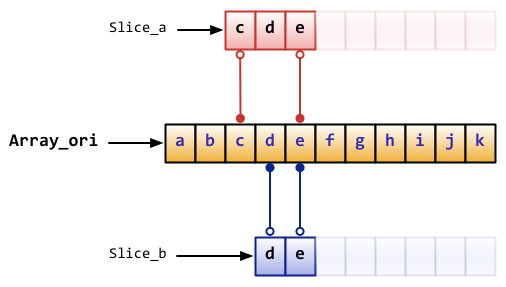
\includegraphics[width=14cm]{2.2.slice.png}
   \label{図2.3}
   \caption{sliceとarrayの対応関係図}
\end{figure}

sliceには便利な操作があります

\begin{itemize}
  \item \texttt{slice}のデフォルト開始位置は0です。\texttt{ar[:n]}などは\texttt{ar[0:n]}と等価です。
  \item \texttt{slice}の2つ目の値のデフォルトは配列の長さです。\texttt{ar[n:]}は\texttt{ar[n:len(ar)]}等価です。
  \item もし配列の中から直接\texttt{slice}を取り出す場合は、\texttt{ar[:]}というような形で指定することができます。なぜならデフォルトのはじめの値は0で2つ目は配列の長さだからです。すなわち、\texttt{ar[0:len(ar)]}と等価となります。
\end{itemize}

ここではより多くの\texttt{slice}の操作についていくつか例を挙げます:

\begin{lstlisting}[numbers=none]
// 配列を宣言
var array = [10]byte{'a', 'b', 'c', 'd', 'e',
                     'f', 'g', 'h', 'i', 'j'}
// sliceを2つ宣言
var aSlice, bSlice []byte

// 便利な操作のデモンストレーション
aSlice = array[:3] // aSlice = array[0:3] と同じ。
// aSliceには以下の要素が含まれます: a,b,c
aSlice = array[5:] // aSlice = array[5:10] と同じ。
// aSliceには以下の要素が含まれます: f,g,h,i,j
aSlice = array[:]  // aSlice = array[0:10] と同じ。
// この場合aSliceにはすべての要素が含まれます。

// sliceからsliceを取り出す
aSlice = array[3:7]  // aSliceには以下の要素が含まれます:
                     // d,e,f,g,len=4,cap=7
bSlice = aSlice[1:3] // bSlice にはaSlice[1], aSlice[2] が
// 含まれそれぞれの要素は以下のとおりです: e,f
bSlice = aSlice[:3]  // bSlice には aSlice[0], aSlice[1],
// aSlice[2] が含まれます。それぞれ以下のとおりです: d,e,f
bSlice = aSlice[0:5] // sliceのsliceに対してcapの
// 範囲内で拡張することができます。
// この時bSliceには以下の要素が含まれます:d,e,f,g,h
bSlice = aSlice[:]   // bSliceにはaSliceのすべての
                     // 要素が含まれます: d,e,f,g
\end{lstlisting}

\texttt{slice}は参照型ですので、この中の要素の値を変更すると、そのほかのすべての参照でも値が変更されます。たとえば上の\texttt{aSlice}と\texttt{bSlice}で、\texttt{aSlice}の中の要素を変更すると、\texttt{bSlice}の対応する値も同時に変更されます。

概念上では、\texttt{slice}は構造体です。この構造体には3つの要素が含まれます: 

\begin{itemize}
  \item 一つはポインタです。配列中の\texttt{slice}が示す開始位置を指しています。
  \item 長さ、つまり\texttt{slice}の長さです。
  \item 最大の長さ、\texttt{slice}の開始位置から配列の最後の位置までの長さです。
\end{itemize}


\begin{lstlisting}[numbers=none]
Array_a := [10]byte{'a', 'b', 'c', 'd', 'e', 'f', 'g', 'h', 'i', 'j'}
Slice_a := Array_a[2:5]
\end{lstlisting}

上のコードの正しい保存構造は下の図に示す通りです。

\begin{figure}[H]
  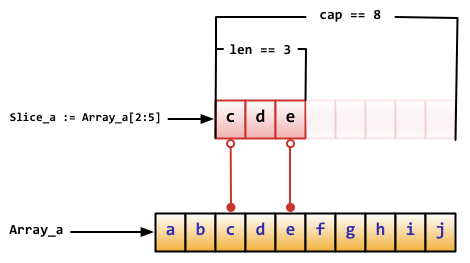
\includegraphics[width=14cm]{2.2.slice2.png}
   \label{図2.4}
   \caption{sliceに対応する配列の情報}
\end{figure}

\texttt{slice}に対しては、いくつかの便利なビルトイン関数があります:

\begin{description}
  \item[\texttt{len}] \texttt{slice}の長さを取得します。
  \item[\texttt{cap}] \texttt{slice}の最大容量を取得します。
  \item[\texttt{append}] \texttt{slice}に対して一つまたは複数の要素を追加します。その後\texttt{slice}と同じ型の\texttt{slice}を返します。
  \item[\texttt{copy}] 関数\texttt{copy}はもとの\texttt{slice}の\texttt{src}を\texttt{dst}に要素をコピーし、コピーした要素の個数を返します。
\end{description}

注:\texttt{append}関数は\texttt{slice}が参照した配列の内容を変更し得ます。そのため、参照先と同一の配列の他の\texttt{slice}にも影響します。 しかし\texttt{slice}の中に余分なスペースが無い(\texttt{(cap-len) == 0})場合、動的なメモリから新たな配列空間が割り当てられます。返される\texttt{slice}配列のポインタはこの空間を指しています。また、もとの配列の内容は変わりません。この配列を参照している他の\texttt{slice}は影響を受けません。

Go1.2より、sliceは三引数のsliceをサポートするようになりました。以前まで我々は以下のような方法でsliceまたはarrayからsliceを取り出していました

\begin{lstlisting}[numbers=none]
var array [10]int
slice := array[2:4]
\end{lstlisting}

この例ではsliceの要素数は8で、新しいバージョンでは以下のように要素数を指定することができます

\begin{lstlisting}[numbers=none]
slice = array[2:4:7]
\end{lstlisting}

上の要素数は\texttt{7-2}、即ち\texttt{5}となります。このように生成された新しいsliceでは最後の3つの要素にアクセスする方法がなくなります。

もしsliceが\texttt{array[:i:j]}のような形式だった場合は、第一引数は空と見なされ、デフォルトの0となります。



\paragraph{map}
\texttt{map}の概念もPythonのディクショナリです。この形式は\texttt{map[keyType]valueType}です。

下のコードをご覧ください。\texttt{map}の読み込みと代入は\texttt{slice}と似ています。\texttt{key}を通して操作します。ただ、\texttt{slice}の\texttt{index}は\texttt{int}型のみになります。\texttt{map}には多くの型があります。\texttt{int}でもかまいませんし、\texttt{string}や\texttt{==}と\texttt{!=}演算子が定義されている全ての型でもかまいません。

\begin{lstlisting}[numbers=none]
  // keyを文字列で宣言します。値はintとなるディクショナリです。
  // この方法は使用される前にmakeで初期化される必要があります。
var numbers map[string]int
// もうひとつのmapの宣言方法
numbers := make(map[string]int)
numbers["one"] = 1  //代入
numbers["ten"] = 10 //代入
numbers["three"] = 3

fmt.Println("3つ目の数字は: ", numbers["three"]) // データの取得
// "3つ目の数字は: 3"という風に出力されます。
\end{lstlisting}

この\texttt{map}は我々が普段目にする表と同じです。左の列に\texttt{key}、右の列に値があります。

mapを使う段階で注意しなければならないことがいくつかあります:

\begin{itemize}
\item \texttt{map}は順序がありません。毎回\texttt{map}の出力は違ったものになるかもしれません。\texttt{index}で値を取得することはできず、かならず\texttt{key}を使うことになります。
\item \texttt{map}の長さは固定ではありません。\texttt{slice}と同じで、参照型の一種です。
\item ビルトインの\texttt{len}関数を\texttt{map}に適用すると、\texttt{map}がもつ\texttt{key}の個数を返します。
\item \texttt{map}の値は簡単に修正することができます。\texttt{numbers["one"]=11}というようにkeyが\texttt{one}のディクショナリの値を\texttt{11}に変えることができます。
\item \texttt{map}は他の基本型と異なり、thread-safeではありません。複数のgo-routineを扱う際には必ずmutex lockメカニズムを使用する必要があります。
\end{itemize}

\texttt{map}の初期化では\texttt{key:val}の方法で初期値を与えることができます。また同時に\texttt{map}には標準で\texttt{key}が存在するか確認する方法が存在します。

\texttt{delete}で\texttt{map}の要素を削除します:

\begin{lstlisting}[numbers=none]
// ディクショナリを初期化します。
rating := map[string]float32{"C":5, "Go":4.5,
                             "Python":4.5, "C++":2 }
// mapは2つの戻り値があります。2つ目の戻り値では、
// もしkeyが存在しなければ、okはfalseに、存在すれ
// ばokはtrueになります。
csharpRating, ok := rating["C#"]
if ok {
fmt.Println("C# is in the map and its rating is ",
            csharpRating)
} else {
fmt.Println("We have no rating associated
             with C# in the map")
}

delete(rating, "C")  // keyがCの要素を削除します。
\end{lstlisting}

上述の通り、\texttt{map}は参照型の一種ですので、もし2つの\texttt{map}が同時に同じポインタを指している場合、一つの変更で、もう一つにも変更が行われます。

\begin{lstlisting}[numbers=none]
m := make(map[string]string)
m["Hello"] = "Bonjour"
m1 := m
m1["Hello"] = "Salut" // この時、m["hello"]の
                // 値もすでにSalutになっています。
\end{lstlisting}





\paragraph{make, new操作}
\texttt{make}はビルトイン型(\texttt{map}、\texttt{slice}および\texttt{channel})のメモリの割り当てです。\texttt{new}は各型のメモリを割り当てます。

ビルトイン関数\texttt{new}は本質的には他の言語で使われる同名の関数と機能が同じです:\texttt{new(T)}はゼロサプレスされた\texttt{T}型のメモリ空間を割り当て、そのアドレスを返します。すなわち\texttt{*T}型の値です。Goの専門用語で言えば、ポインタを返すということです。新たに割り当てられた型\texttt{T}のゼロ値です。とても重要なことに:

\begin{quote}
\texttt{new}はポインタを返します。
\end{quote}

ビルトイン関数\texttt{make(T, args)}と\texttt{new(T)}は異なる機能を持っています。makeは\texttt{slice}、\texttt{map}または\texttt{channel}を作成し、初期値(非ゼロ値)を持つ\texttt{T}型を返すのみで、\texttt{*T}ではありません。本質的には、この3つの型が異なる点はデータ構造を指し示す参照が使用される前に初期化されているということです。例えば、データ(内部\texttt{array})を指し示すポインタ、長さ,容量による3点で記述される\texttt{slice}の各項目が初期化される前は、\texttt{slice}は\texttt{nil}です。\texttt{slice}, \texttt{map}, \texttt{channel}にとって、makeは内部のデータ構造を初期化し、適当な値で埋め尽くされます。


\begin{quote}
\texttt{make}は初期化後の(非ゼロの)値を返します。
\end{quote}




\begin{figure}[H]
  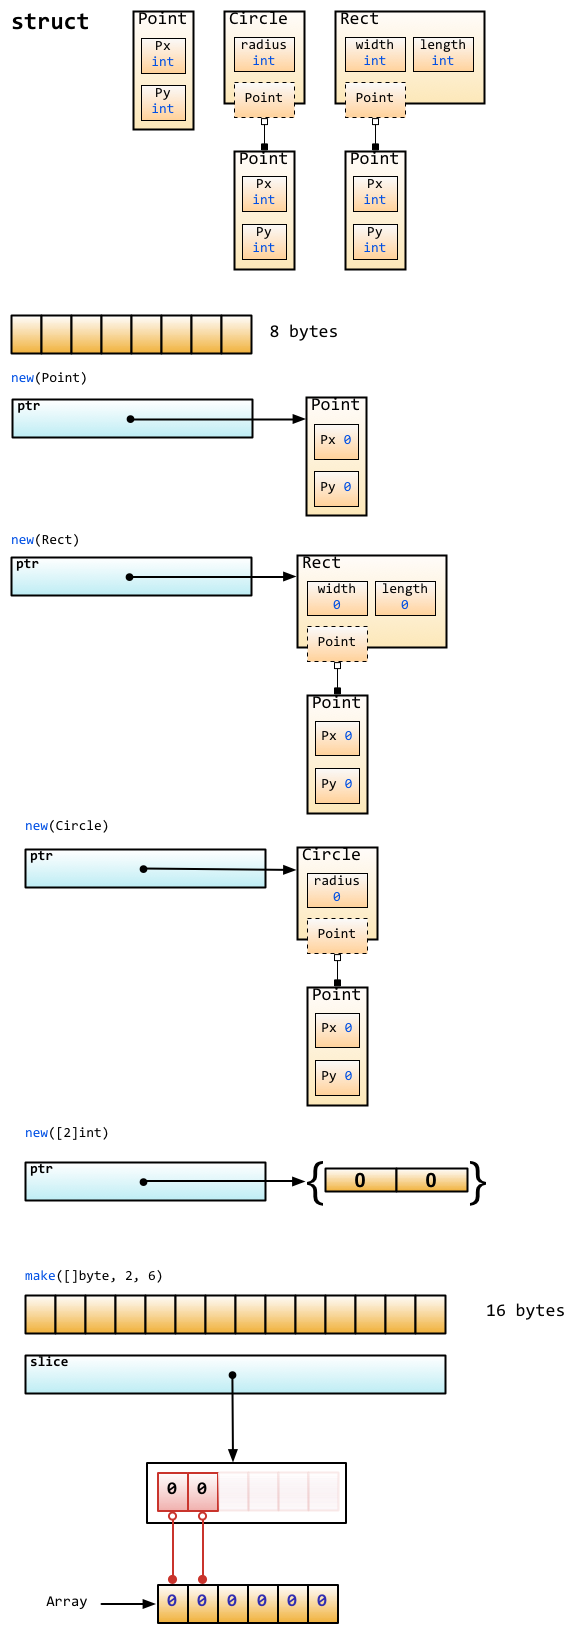
\includegraphics[width=7cm]{2.2.makenew.png}
   \label{図2.5}
   \caption{makeとnewの低レイヤでのメモリの割り当て}
\end{figure}

\subsubsection{ゼロ値}
"ゼロ値"というのは何も空の値ではありません。これは一種の"変数が埋めらる前"のデフォルト値であり、通常は0です。 それぞれの型のゼロ値は以下の通りです


\begin{lstlisting}[numbers=none]
int     0
int8    0
int32   0
int64   0
uint    0x0
rune    0 //runeの実際の型は int32 です。
byte    0x0 // byteの実際の型は uint8 です。
float32 0 //長さは 4 byte
float64 0 //長さは 8 byte
bool    false
string  ""
\end{lstlisting}


\subsection{フローと関数}
この節ではGoの中のフロー制御と関数操作についてご紹介します。

\subsubsection{フロー制御}
フロー制御はプログラム言語の中の最も偉大な発明です。なぜならこれがあるだけで、あなたはとても簡単なフローの記述でとても複雑なロジックを表現できるからです。Goではフロー制御は3つの部分から成ります:条件判断、ループ制御及び無条件ジャンプです。

\paragraph{if}
\texttt{if}はあらゆるプログラミング言語の中で最もよく見かけるものかもしれません。この文法は大雑把に言えば:もし条件を満足しなければ何々を行い、そうでなければまたもう一つ別のことをやるということです。

Goの中では\texttt{if}分岐の文法の中は括弧で括る必要はありません。以下のコードをご覧ください。

\begin{lstlisting}[numbers=none]
if x > 10 {
    fmt.Println("x is greater than 10")
} else {
    fmt.Println("x is less than 10")
}
\end{lstlisting}

Goの\texttt{if}はすごいことに、条件分岐の中で変数を宣言できます。この変数のスコープはこの条件ロジックブロック内のみ存在し、他の場所では作用しません。以下に示します

\begin{lstlisting}[numbers=none]
// 取得値xを計算し、xの大きさを返します。
// 10以上かどうかを判断します。
if x := computedValue(); x > 10 {
    fmt.Println("x is greater than 10")
} else {
    fmt.Println("x is less than 10")
}

/ /ここではもしこのようにコールしてしまうとコンパイルエラー
// となります。xは条件の中の変数だからです。
fmt.Println(x)
\end{lstlisting}

この条件の時は以下のようになります:

\begin{lstlisting}[numbers=none]
if integer == 3 {
    fmt.Println("The integer is equal to 3")
} else if integer < 3 {
    fmt.Println("The integer is less than 3")
} else {
    fmt.Println("The integer is greater than 3")
}
\end{lstlisting}


\paragraph{goto}
Goには\texttt{goto}句があります- - ぜひ賢く使ってください。\texttt{goto}は必ず事前に関数内で定義したタグにジャンプします。例えばこのようなループがあったと仮定します:

\begin{lstlisting}[numbers=none]
func myFunc() {
    i := 0
Here:   //この行の最初の単語はコロンを
        // 最後に持ってくることでタグとなります。
    println(i)
    i++
    goto Here   //Hereにジャンプします。
}
\end{lstlisting}

\begin{quote}
タグの名前は大文字小文字を区別します。
\end{quote}


\paragraph{for}
Goにで最も強力なロジックコントロールといえば、\texttt{for}です。これはループでデータを読むのに使えます。\texttt{while}でロジックをコントロールしても構いません。イテレーション操作も行えます。文法は以下の通りです:

\begin{lstlisting}[numbers=none]
for expression1; expression2; expression3 {
    //...
}
\end{lstlisting}

\texttt{expression1}、\texttt{expression2}と\texttt{expression3}はどれも式です。この中で\texttt{expression1}と\texttt{expression3}は変数宣言または関数のコールの戻り値のようなものです。\texttt{expression2}は条件判断に用いられます。\texttt{expression1}はループの開始前にコールされます。\texttt{expression3}は毎回ループする際の終了時にコールされます。

だらだら喋るよりも例を見たほうが早いでしょう。以下に例を示します:


\begin{lstlisting}[numbers=none]
package main
import "fmt"

func main(){
    sum := 0;
    for index:=0; index < 10 ; index++ {
        sum += index
    }
    fmt.Println("sum is equal to ", sum)
}
// 出力:sum is equal to 45
\end{lstlisting}

時々複数の代入操作を行いたい時があります。Goのなかには\texttt{,}という演算子はないので、平行して代入することができます。\texttt{i, j = i+1, j-1}

時々\texttt{expression1}と\texttt{expression3}を省略します:


\begin{lstlisting}[numbers=none]
sum := 1
for ; sum < 1000;  {
    sum += sum
}
\end{lstlisting}

この中で\texttt{;}は省略することができます。ですので下のようなコードになります。どこかで見た覚えはありませんか?そう、これは\texttt{while}の機能です。

\begin{lstlisting}[numbers=none]
sum := 1
for sum < 1000 {
    sum += sum
}
\end{lstlisting}

ループの中では\texttt{break}と\texttt{continue}という2つのキーとなる操作があります。\texttt{break}操作は現在のループから抜け出します。\texttt{continue}は次のループに飛び越えます。ネストが深い場合、\texttt{break}はタグと組み合わせて使用することができます。つまり、タグが指定する位置までジャンプすることになります。詳細は以下の例をご覧ください。

\begin{lstlisting}[numbers=none]
for index := 10; index>0; index-- {
    if index == 5{
        break // またはcontinue
    }
    fmt.Println(index)
}
// breakであれば10、9、8、7、6が出力されます。
// continueの場合は10、9、8、7、6、4、3、2、1が出力されます。
\end{lstlisting}

\texttt{break}と\texttt{continue}はタグを添えることができます。複数ネストしたループで外側のループからジャンプする際に使用されます。

\texttt{for}は\texttt{range}と組み合わせて\texttt{array}、\texttt{slice}、\texttt{map}、\texttt{string}のデータを読み込むことができます:

\begin{lstlisting}[numbers=none]
for k,v:=range map {
    fmt.Println("map's key:",k)
    fmt.Println("map's val:",v)
}
\end{lstlisting}

Goは"複数の戻り値"をサポートしていますが、"宣言して使用されていない"変数に対してコンパイラはエラーを出力します。このような状況では\texttt{\_}を使って必要のない戻り値を捨てる事ができます。 例えば

\begin{lstlisting}[numbers=none]
for _, v := range map{
    fmt.Println("map's val:", v)
}
\end{lstlisting}



\paragraph{switch}
時々たくさんの\texttt{if-else}を書くことでロジック処理を行いたくなるかもしれません。コードは非常に醜く冗長になります。またメンテナンスも容易ではなくなるので、\texttt{switch}を使って解決することができます。この文法は以下のようなものです

\begin{lstlisting}[numbers=none]
switch sExpr {
case expr1:
    some instructions
case expr2:
    some other instructions
case expr3:
    some other instructions
default:
    other code
}
\end{lstlisting}

\texttt{sExpr}と\texttt{expr1}、\texttt{expr2}、\texttt{expr3}の型は一致させる必要があります。Goの\texttt{switch}は非常に使い勝手がよく、式は必ずしも定数や整数である必要はありません。実行のプロセスは上から下まで、マッチする項目が見つかるまで行われます。もし\texttt{switch}に式がなければ、\texttt{true}とマッチします。

\begin{lstlisting}[]
i := 10
switch i {
case 1:
    fmt.Println("i is equal to 1")
case 2, 3, 4:
    fmt.Println("i is equal to 2, 3 or 4")
case 10:
    fmt.Println("i is equal to 10")
default:
    fmt.Println("All I know is that i is an integer")
}
\end{lstlisting}

5行目で、いくつもの値を\texttt{case}の中に集めています。また同時に、Goの\texttt{switch}はデフォルトで\texttt{case}の最後に\texttt{break}があることになっているので、マッチに成功した後は他のcaseが実行されることはなく、\texttt{switch}全体から抜け出します。ただし、\texttt{fallthrough}を使用することであとに続くcaseコードを強制的に実行させることができます。

\begin{lstlisting}[numbers=none]
integer := 6
switch integer {
    case 4:
    fmt.Println("The integer was <= 4")
    fallthrough
    case 5:
    fmt.Println("The integer was <= 5")
    fallthrough
    case 6:
    fmt.Println("The integer was <= 6")
    fallthrough
    case 7:
    fmt.Println("The integer was <= 7")
    fallthrough
    case 8:
    fmt.Println("The integer was <= 8")
    fallthrough
    default:
    fmt.Println("default case")
}
\end{lstlisting}

上のプログラムは以下のように出力します

\begin{lstlisting}[numbers=none]
The integer was <= 6
The integer was <= 7
The integer was <= 8
default case
\end{lstlisting}


\subsubsection{関数}
関数はGoの中心的な設計です。キーワード\texttt{func}によって宣言します。形式は以下の通り:

\begin{lstlisting}[numbers=none]
func funcName(input1 type1, input2 type2)
                (output1 type1, output2 type2) {
    //ここはロジック処理のコードです。
    //複数の値を戻り値とします。
    return value1, value2
}
\end{lstlisting}

上のコードから次のようなことが分かります

\begin{itemize}
\item キーワード\texttt{func}で\texttt{funcName}という名前の関数を宣言します。
\item 関数はひとつまたは複数の引数をとることができ、各引数の後には型が続きます。\texttt{,}をデリミタとします。
\item 関数は複数の戻り値を持ってかまいません。
\item 上の戻り値は2つの変数\texttt{output1}と\texttt{output2}であると宣言されています。もしあなたが宣言したくないというのであればそれでもかみません。直接2つの型です。
\item もしひとつの戻り値しか存在せず、また戻り値の変数が宣言されていなかった場合、戻り値の括弧を省略することができます。
\item もし戻り値が無ければ、最後の戻り値の情報も省略することができます。
\item もし戻り値があれば、関数の中でreturn文を追加する必要があります。
\end{itemize}

以下では実際に関数の例を応用しています(Maxの値を計算します)

\begin{lstlisting}[numbers=none]
package main
import "fmt"

// a、bの中から最大値を返します。
func max(a, b int) int {
    if a > b {
        return a
    }
    return b
}

func main() {
    x := 3
    y := 4
    z := 5

    max_xy := max(x, y) //関数max(x, y)をコール
    max_xz := max(x, z) //関数max(x, z)をコール

    fmt.Printf("max(%d, %d) = %d\n", x, y, max_xy)
    fmt.Printf("max(%d, %d) = %d\n", x, z, max_xz)
    fmt.Printf("max(%d, %d) = %d\n", y, z, max(y,z))
                   // 直接コールしてもかまいません。
}
\end{lstlisting}

上では\texttt{max}関数に2つの引数があることがわかります。この型はどれも\texttt{int}です。第一引数の型は省略することができます(つまり、a,b int,でありa int, b intではありません)、デフォルトは直近の型です。2つ以上の同じ型の変数または戻り値も同じです。同時に戻り値がひとつであることに注意してください。これは省略記法です。


\paragraph{複数の戻り値}
Go言語はCに比べ先進的な特徴を持っています。関数が複数の戻り値を持てるのもその一つです。

コードの例を見てみましょう

\begin{lstlisting}[numbers=none]
package main
import "fmt"

//A+B と A*B を返します
func SumAndProduct(A, B int) (int, int) {
    return A+B, A*B
}

func main() {
    x := 3
    y := 4

    xPLUSy, xTIMESy := SumAndProduct(x, y)

    fmt.Printf("%d + %d = %d\n", x, y, xPLUSy)
    fmt.Printf("%d * %d = %d\n", x, y, xTIMESy)
}
\end{lstlisting}

上の例では直接2つの引数を返しました。当然引数を返す変数に命名してもかまいません。この例では2つの型のみ使っていますが、下のように定義することもできます。値が返る際は変数名を付けなくてかまいません。なぜなら関数の中で直接初期化されているからです。しかしもしあなたの関数がエクスポートされるのであれば(大文字からはじまります)オフィシャルではなるべく戻り値に名前をつけるようお勧めしています。なぜなら名前のわからない戻り値はコードをより簡潔なものにしますが、生成されるドキュメントの可読性がひどくなるからです。

\begin{lstlisting}[numbers=none]
func SumAndProduct(A, B int) (add int, Multiplied int) {
    add = A+B
    Multiplied = A*B
    return
}
\end{lstlisting}


\paragraph{可変長引数}
Goの関数は可変長引数をサポートしています。可変長引数を受け付ける関数は不特定多数の引数があります。これを実現するために、関数が可変長引数を受け取れるよう定義する必要があります:

\begin{lstlisting}[numbers=none]
func myfunc(arg ...int) {}
\end{lstlisting}

\texttt{arg ...int}はGoにこの関数が不特定多数の引数を受け付けることを伝えます。ご注意ください。この引数の型はすべて\texttt{int}です。関数ブロックの中で変数\texttt{arg}は\texttt{int}の\texttt{slice}となります。

\begin{lstlisting}[numbers=none]
for _, n := range arg {
    fmt.Printf("And the number is: %d\n", n)
}
\end{lstlisting}


\paragraph{値渡しと参照渡し}
引数をコールされる関数の中に渡すとき、実際にはこの値のコピーが渡されます。コールされる関数の中で引数に修正をくわえても、関数をコールした実引き数には何の変化もありません。数値の変化はコピーの上で行われるだけだからです。

この内容を検証するために、ひとつ例を見てみましょう


\begin{lstlisting}[numbers=none]
package main
import "fmt"

//引数+1を行う、簡単な関数
func add1(a int) int {
    a = a+1 // aの値を変更します。
    return a //新しい値を返します。
}

func main() {
    x := 3

    fmt.Println("x = ", x)  // "x = 3"と出力するはずです。

    x1 := add1(x)  //add1(x) をコールします。

    fmt.Println("x+1 = ", x1)
    // "x+1 = 4" と出力するはずです。

    fmt.Println("x = ", x)
    // "x = 3" と出力するはずです。
}
\end{lstlisting}

どうです?\texttt{add1}関数をコールし、\texttt{add1}のなかで\texttt{a = a+1}の操作を実行したとしても、上述の\texttt{x}変数には何の変化も発生しません。

理由はとても簡単です:\texttt{add1}がコールされた際、\texttt{add1}が受け取る引数は\texttt{x}そのものではなく、\texttt{x}のコピーだからです。

もし本当にこの\texttt{x}そのものを渡したくなったらどうするの?と疑問に思うかもしれません。

この場合いわゆるポインタにまで話がつながります。我々は変数がメモリの中のある特定の位置に存在していることを知っています。変数を修正するということはとどのつまり変数のアドレスにあるメモリを修正していることになります。\texttt{add1}関数が\texttt{x}変数のアドレスを知ってさえいれば、\texttt{x}変数の値を変更することが可能です。そのため、我々は\texttt{x}の存在するアドレスである\texttt{\&x}を関数に渡し、関数の変数の型を\texttt{int}からポインタ変数である\texttt{*int}に変更します。これで関数の中で\texttt{x}の値を変更することができるようになりました。この時関数は依然としてコピーにより引数を受け渡しますが、コピーしているのはポインタになります。以下の例をご覧ください。

\begin{lstlisting}[numbers=none]
package main
import "fmt"

//引数に+1を行う簡単な関数
func add1(a *int) int { // ご注意ください。
    *a = *a+1 // aの値を修正しています。
    return *a // 新しい値を返します。
}

func main() {
    x := 3

    fmt.Println("x = ", x)  // "x = 3"と出力するはずです。

    x1 := add1(&x)
    // add1(&x) をコールしてxのアドレスを渡します。

    fmt.Println("x+1 = ", x1)
    // "x+1 = 4"を出力するはずです。

    fmt.Println("x = ", x)
    // "x = 4"を出力するはずです。
}
\end{lstlisting}

このように\texttt{x}を修正するという目的に到達しました。では、ポインタを渡す長所はなんなのでしょうか?

\begin{itemize}
  \item ポインタを渡すことで複数の関数が同じオブジェクトに対して操作を行うことができます。
  \item ポインタ渡しは比較的軽いです(8バイト)、ただのメモリのアドレスです。ポインタを使って大きな構造体を渡すことができます。もし値渡しを行なっていたら、相対的にもっと多くのシステムリソース(メモリと時間)を毎回のコピーで消費することになります。そのため大きな構造体を渡す際は、ポインタを使うのが賢い選択というものです。
  \item Go言語の\texttt{channel}、\texttt{slice}、\texttt{map}の3つの型はメカニズムを実現するポインタのようなものです。ですので、直接渡すことができますので、アドレスを取得してポインタを渡す必要はありません。(注:もし関数が\texttt{slice}の長さを変更する場合はアドレスを取得し、ポインタを渡す必要があります。)
\end{itemize}


\paragraph{defer}
Go言語のすばらしいデザインの中に、遅延(defer)文法があります。関数の中でdefer文を複数追加することができます。関数が最後まで実行された時、このdefer文が逆順に実行されます。最後にこの関数が返ります。特に、リソースをオープンする操作を行なっているようなとき、エラーの発生に対してロールバックし、必要なリソースをクローズする必要があるかと思います。さもなければとても簡単にリソースのリークといった問題を引き起こすことになります。我々はリソースを開く際は一般的に以下のようにします:

\begin{lstlisting}[numbers=none]
func ReadWrite() bool {
    file.Open("file")
// 何かを行う
    if failureX {
        file.Close()
        return false
    }

    if failureY {
        file.Close()
        return false
    }

    file.Close()
    return true
}
\end{lstlisting}

上のコードはとても多くの重複がみられます。Goの\texttt{defer}はこの問題を解決します。これを使用した後、コードは減るばかりでなく、プログラムもよりエレガントになります。\texttt{defer}の後に指定された関数が関数を抜ける前にコールされます。

\begin{lstlisting}[numbers=none]
func ReadWrite() bool {
    file.Open("file")
    defer file.Close()
    if failureX {
        return false
    }
    if failureY {
        return false
    }
    return true
}
\end{lstlisting}

もし\texttt{defer}を多用する場合は、\texttt{defer}はLIFOモードが採用されます。そのため、以下のコードは\texttt{4 3 2 1 0}を出力します。

\begin{lstlisting}[numbers=none]
for i := 0; i < 5; i++ {
    defer fmt.Printf("%d ", i)
}
\end{lstlisting}


\paragraph{値、型としての関数}
Goでは関数も変数の一種です。\texttt{type}を通して定義します。これは全て同じ引数と同じ戻り値を持つ一つの型です。


\begin{lstlisting}[numbers=none]
type typeName func(input1 inputType1 ,
                   input2 inputType2 [, ...])
                     (result1 resultType1 [, ...])
\end{lstlisting}

関数を型として扱うことにメリットはあるのでしょうか?ではこの型の関数を値として渡してみましょう。以下の例をご覧ください。

\begin{lstlisting}[numbers=none]
package main
import "fmt"

type testInt func(int) bool // 関数の型を宣言します。

func isOdd(integer int) bool {
    if integer%2 == 0 {
        return false
    }
    return true
}

func isEven(integer int) bool {
    if integer%2 == 0 {
        return true
    }
    return false
}

// ここでは宣言する関数の型を引数のひとつとみなします。

func filter(slice []int, f testInt) []int {
    var result []int
    for _, value := range slice {
        if f(value) {
            result = append(result, value)
        }
    }
    return result
}

func main(){
    slice := []int {1, 2, 3, 4, 5, 7}
    fmt.Println("slice = ", slice)
    odd := filter(slice, isOdd)    // 関数の値渡し
    fmt.Println("Odd elements of slice are: ", odd)
    even := filter(slice, isEven)  // 関数の値渡し
    fmt.Println("Even elements of slice are: ", even)
}
\end{lstlisting}

共有のインターフェースを書くときに関数を値と型にみなすのは非常に便利です。上の例で\texttt{testInt}という型は関数の型の一つでした。ふたつの\texttt{filter}関数の引数と戻り値は\texttt{testInt}の型と同じですが、より多くのロジックを実現することができます。このように我々のプログラムをより優れたものにすることができます。


\paragraph{PanicとRecover}
GoにはJavaのような例外処理はありません。例外を投げないのです。その代わり、\texttt{panic}と\texttt{recover}を使用します。ぜひ覚えておいてください、これは最後の手段として使うことを。つまり、あなたのコードにあってはなりません。もしくは\texttt{panic}を極力減らしてください。これは非常に強力なツールです。賢く使ってください。では、どのように使うのでしょうか?


Panic
\begin{quote}
ビルトイン関数です。オリジナルの処理フローを中断させることができます。パニックが発生するフローの中に入って関数\texttt{F}が\texttt{panic}をコールします。このプロセスは継続して実行されます。一旦\texttt{panic}の\texttt{goroutine}が発生すると、コールされた関数がすべて返ります。この時プログラムを抜けます。パニックは直接\texttt{panic}をコールします。実行時にエラーを発生させてもかまいません。例えば配列の境界を超えてアクセスする、などです。
\end{quote}


Recover
\begin{quote}
ビルトイン関数です。パニックを発生させるフローの\texttt{goroutine}を復元することができます。\texttt{recover}は遅延関数の中でのみ有効です。通常の実行中、\texttt{recover}をコールすると\texttt{nil}が返ります。他には何の効果もありません。もし現在の\texttt{goroutine}がパニックに陥ったら\texttt{recover}をコールして、\texttt{panic}の入力値を補足し、正常な実行に復元することができます。
\end{quote}

下の関数のフローの中でどのように\texttt{panic}を使うかご覧ください

\begin{lstlisting}[numbers=none]
var user = os.Getenv("USER")

func init() {
    if user == "" {
        panic("no value for $USER")
    }
}
\end{lstlisting}

この関数は引数となっている関数が実行時に\texttt{panic}を発生するか検査します:

\begin{lstlisting}[numbers=none]
func throwsPanic(f func()) (b bool) {
    defer func() {
        if x := recover(); x != nil {
            b = true
        }
    }()
    f() // 関数fを実行します。もしfの中でpanicが出現したら、
        // 復元を行うことができます。
    return
}
\end{lstlisting}


\paragraph{\texttt{main}関数と\texttt{init}関数}
Goでは2つの関数が予約されています:\texttt{init}関数(すべての\texttt{package}で使用できます)と\texttt{main}関数(\texttt{package main}でしか使用できません)です。この2つの関数は定義される際いかなる引数と戻り値も持ちません。\texttt{package}のなかで複数の\texttt{init}関数を書いたとしても、もちろん可読性か後々のメンテナンス性に対してですが、\texttt{package}の中では各ファイルに一つだけの\texttt{init}関数を書くよう強くおすすめします。

Goのプログラムは自動で\texttt{init()}と\texttt{main()}をコールしますので、どこかでこの2つの関数をコールする必要はありません。各\texttt{package}の\texttt{init}関数はオプションです。しかし\texttt{package main}は必ず一つ\texttt{main}関数を含まなければなりません。

プログラムの初期化と実行はすべて\texttt{main}パッケージから始まります。もし\texttt{main}パッケージが他のパッケージをインポートしていたら、コンパイル時にその依存パッケージがインポートされます。あるパッケージが複数のパッケージに同時にインポートされている場合は、先にその他のパッケージがインポートされ、その後このパッケージの中にあるパッケージクラス定数と変数が初期化されます。次にinit関数が(もしあれば)実行され、最後に\texttt{main}関数が実行されます。以下の図で実行過程を詳しくご説明しています。

\begin{figure}[H]
  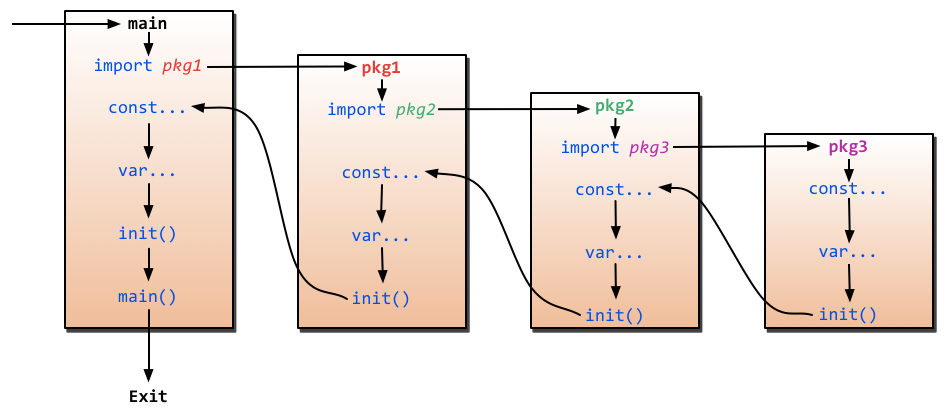
\includegraphics[width=14cm]{2.3.init.png}
   \label{図2.6}
   \caption{main関数によるパッケージのインポートと初期化過程の図}
\end{figure}

\paragraph{import}
Goのコードを書いている時は、importコマンドによってパッケージファイルをインポートすることがよくあります。私達が通常使う方法は以下を参考にしてください:


\begin{lstlisting}[numbers=none]
import(
    "fmt"
)
\end{lstlisting}

その後コードの中では以下のような方法でコールすることができます。

\begin{lstlisting}[numbers=none]
fmt.Println("hello world")
\end{lstlisting}

上のfmtはGo言語の標準ライブラリです。実は\texttt{GOROOT}環境変数で指定されたディレクトリの下にこのモジュールが加えられています。当然Goのインポートは以下のような2つの方法で自分の書いたモジュールを追加することができます:

\begin{enumerate}
  \item 相対パス\\ import "./model" //カレントファイルと同じディレクトリにあるmodelディレクトリ、ただし、この方法によるimportはおすすめしません。
  \item 絶対パス\\ import "shorturl/model" //gopath/src/shorturl/modelモジュールを追加します。
\end{enumerate}

ここではimportの通常のいくつかの方法をご説明しました。ただ他にも特殊なimportがあります。新人を悩ませる方法ですが、ここでは一つ一つ一体何がどうなっているのかご説明しましょう

\begin{enumerate}
  \item ドット操作\\ 時々、以下のようなパッケージのインポート方法を見ることがあります
    \begin{lstlisting}[numbers=none]
import(
    . "fmt"
)
    \end{lstlisting}
 このドット操作の意味はこのパッケージがインポートされた後このパッケージの関数をコールする際、パッケージ名を省略することができます。つまり、前であなたがコールしたようなfmt.Println("hello world")はPrintln("hello world")というように省略することができます。
  \item エイリアス操作\\ エイリアス操作はその名の通りパッケージ名に他の覚えやすい名前をつけることができます。
    \begin{lstlisting}[numbers=none]
import(
    f "fmt"
)
    \end{lstlisting}
エイリアス操作の場合パッケージ関数をコールする際プレフィックスが自分たちのものになります。すなわち、f.Println("hello world")
  \item \_操作\\ この操作は通常とても理解しづらい方法です。以下のimportをご覧ください。
    \begin{lstlisting}[numbers=none]
import (
    "database/sql"
    _ "github.com/ziutek/mymysql/godrv"
)
    \end{lstlisting}
\_操作はこのパッケージをインポートするだけでパッケージの中の関数を直接使うわけではなく、このパッケージの中にあるinit関数をコールします。
\end{enumerate}





\subsection{struct型}
\subsubsection{struct}
Go言語では、Cや他の言語と同じように、他の型の属性やフィールドのコンテナとして新しい型を宣言することができます。例えば、一個人のエンティティを表している\texttt{person}型を作成することができます。このエンティティは属性を持っています:性別と年齢です。このような型は\texttt{struct}と呼ばれます。以下にコードを示します:

\begin{lstlisting}[numbers=none]
type person struct {
    name string
    age int
}
\end{lstlisting}

お分かりいただけましたでしょうか?structの宣言はこのように簡単です。上の型は2つのフィールドを持っています。

\begin{itemize}
  \item string型のフィールドnameはユーザの名前を保存するプロパティです。
  \item int型のフィールドageはユーザの年齢を保存するプロパティです。
\end{itemize}

どのようにstructは使用されるのでしょうか?下のコードをご覧ください。

\begin{lstlisting}[numbers=none]
type person struct {
    name string
    age int
}

var P person  // Pは現在person型の変数です。

P.name = "Astaxie"
// "Astaxie"を変数Pのnameプロパティに代入します。
P.age = 25  // "25"を変数Pのageプロパティに代入します。
fmt.Printf("The person's name is %s", P.name)
// Pのnameプロパティにアクセスします。
\end{lstlisting}

上のようなPの宣言以外に他にもいくつかの宣言方法があります。

\begin{enumerate}
  \item 順序にしたがって初期化する。\\ P := person\{"Tom", 25\}
  \item \texttt{field:value}の方法によって初期化します。この場合は順序は任意でかまいません。\\ P := person\{age:24, name:"Tom"\}
  \item もちろん\texttt{new}関数を通してポインタを作ることもできます。このPの型は*personです。\\ P := new(person)
\end{enumerate}

以下ではひと通りのstructの使用例をご説明します。

\begin{lstlisting}[numbers=none]
package main
import "fmt"

// 新しい型を宣言します。
type person struct {
    name string
    age int
}

// 二人の年齢を比較します。
// 年齢が大きい方の人を返し、また年齢差も返します。
// structも値渡しです。
func Older(p1, p2 person) (person, int) {
    if p1.age>p2.age {  // p1とp2の二人の年齢を比較します。
        return p1, p1.age-p2.age
    }
    return p2, p2.age-p1.age
}

func main() {
    var tom person

    // 初期値を代入します。
    tom.name, tom.age = "Tom", 18

    // 2つのフィールドを明確に初期化します。
    bob := person{age:25, name:"Bob"}

    // structの定義の順番に従って初期化します。
    paul := person{"Paul", 43}

    tb_Older, tb_diff := Older(tom, bob)
    tp_Older, tp_diff := Older(tom, paul)
    bp_Older, bp_diff := Older(bob, paul)

    fmt.Printf("Of %s and %s, %s is older by %d years\n",
        tom.name, bob.name, tb_Older.name, tb_diff)

    fmt.Printf("Of %s and %s, %s is older by %d years\n",
        tom.name, paul.name, tp_Older.name, tp_diff)

    fmt.Printf("Of %s and %s, %s is older by %d years\n",
        bob.name, paul.name, bp_Older.name, bp_diff)
}
\end{lstlisting}

\subsubsection{structの匿名フィールド}
上でstructをどのように定義するかご紹介しました。定義する際はフィールド名とその型が一つ一つ対応しています。実はGoは型だけの定義もサポートしています。これはフィールド名を書かない方法ではなく、匿名フィールドです。組み込みフィールドとも呼ばれます。

匿名フィールドがstructである場合、このstructがもつすべてのフィールドは隠されたまま現在定義しているこのstructに導入されます。

ひとつ例をお見せしましょう。上の説明がより具体的になります。

\begin{lstlisting}[numbers=none]
package main
import "fmt"

type Human struct {
    name string
    age int
    weight int
}

type Student struct {
    Human  // 匿名フィールド、デフォルトでStudentは
           // Humanのすべてのフィールドを含むことになります。
    speciality string
}

func main() {
    // 学生を一人初期化します。
    mark := Student{Human{"Mark", 25, 120},
                    "Computer Science"}

    // 対応するフィールドにアクセスします。
    fmt.Println("His name is ", mark.name)
    fmt.Println("His age is ", mark.age)
    fmt.Println("His weight is ", mark.weight)
    fmt.Println("His speciality is ", mark.speciality)
    // 対応するメモ情報を修正します。
    mark.speciality = "AI"
    fmt.Println("Mark changed his speciality")
    fmt.Println("His speciality is ", mark.speciality)
    // 彼の年齢情報を修正します。
    fmt.Println("Mark become old")
    mark.age = 46
    fmt.Println("His age is", mark.age)
    // 体重情報も修正します。
    fmt.Println("Mark is not an athlet anymore")
    mark.weight += 60
    fmt.Println("His weight is", mark.weight)
}
\end{lstlisting}

\begin{figure}[H]
  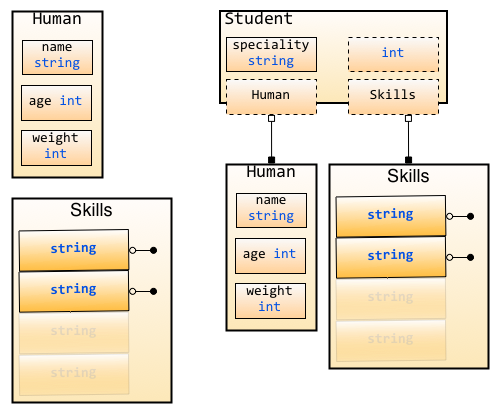
\includegraphics[width=14cm]{2.4.student_struct.png}
   \label{図2.7}
   \caption{StudentとHumanの継承方法}
\end{figure}

Studentがageとnameの属性にアクセスする際、あたかも自分のフィールドであるかのようにアクセスしたのをご覧いただけるかと思います。そうです。匿名フィールドというのはこういうものです。フィールドの継承を実現できるのです。これってクールじゃないですか?もっとクールにする方法もありますよ。studentはHumanのフィールド名でアクセスできます。下のコードを御覧ください。ほら、とってもクールでしょ?

\begin{lstlisting}[numbers=none]
mark.Human = Human{"Marcus", 55, 220}
mark.Human.age -= 1
\end{lstlisting}

匿名によるアクセスとフィールドの修正はとても便利です。でも単なるstructのフィールドですから、すべてのビルトイン型と自分で定義した型をすべて匿名フィールドとみなすことができます。下の例をご覧ください。

\begin{lstlisting}[numbers=none]
package main
import "fmt"

type Skills []string

type Human struct {
    name string
    age int
    weight int
}

type Student struct {
    Human  // 匿名フィールド、struct
    Skills // 匿名フィールド、自分で定義した型。string slice
    int    // ビルトイン型を匿名フィールドとします。
    speciality string
}

func main() {
    // 学生Jannを初期化します。
    jane := Student{Human:Human{"Jane", 35, 100},
                    speciality:"Biology"}
    // ここで対応するフィールドにアクセスしてみます。
    fmt.Println("Her name is ", jane.name)
    fmt.Println("Her age is ", jane.age)
    fmt.Println("Her weight is ", jane.weight)
    fmt.Println("Her speciality is ", jane.speciality)
    // 彼のskill技能フィールドを修正します。
    jane.Skills = []string{"anatomy"}
    fmt.Println("Her skills are ", jane.Skills)
    fmt.Println("She acquired two new ones ")
    jane.Skills = append(jane.Skills, "physics", "golang")
    fmt.Println("Her skills now are ", jane.Skills)
    // 匿名ビルトイン型のフィールドを修正します。
    jane.int = 3
    fmt.Println("Her preferred number is", jane.int)
}
\end{lstlisting}

上の例のとおり、structはstructを匿名フィールドとするだけでなく、自分で定義した型やビルトイン型も匿名フィールドとすることができます。また、対応するフィールド上で関数操作を行うこともできます(例えば例の中のappendです)。

ここで一つ疑問がでてきます:もしhumanにphoneというフィールドがあったとすると、studentもphoneと呼ばれるフィールドができます。これはどうすべきでしょうか?

Goでは簡単にこの問題を解決することができます。外側が優先的にアクセスされますので、\texttt{student.phone}とアクセスした場合studentの中のフィールドにアクセスし、humanのフィールドにはアクセスしません。

このように匿名フィールドを通じてフィールドを継承することができます。当然もしあなたが対応する匿名型のフィールドにアクセスしたくなったら、匿名フィールドの名前からアクセスすることができます。下の例をご覧ください。

\begin{lstlisting}[numbers=none]
package main
import "fmt"

type Human struct {
    name string
    age int
    phone string  // Human型がもつフィールド
}

type Employee struct {
    Human  // 匿名フィールドHuman
    speciality string
    phone string  // 社員のphoneフィールド
}

func main() {
    Bob := Employee{Human{"Bob", 34, "777-444-XXXX"},
                          "Designer", "333-222"}
    fmt.Println("Bob's work phone is:", Bob.phone)
    // もし我々がHumanのphoneフィールドにアクセスする場合は
    fmt.Println("Bob's personal phone is:",
                Bob.Human.phone)
}
\end{lstlisting}



\subsection{オブジェクト指向}
前の2つの章で関数とstructをご紹介しました。関数をstructのフィールドとして処理したくなったんじゃないですか?今日は関数のもう一つの形態についてご説明します。受け取り手のいる関数で、我々が\texttt{method}とよんでいるものです。

\subsubsection{method}
今、このような状況にいると仮定します。あなたは長方形というstructを定義してこの面積を求めようとしています。我々の一般的な思考回路に基づけば下のような方法で実現するでしょう。


\begin{lstlisting}[numbers=none]
package main
import "fmt"

type Rectangle struct {
    width, height float64
}

func area(r Rectangle) float64 {
    return r.width*r.height
}

func main() {
    r1 := Rectangle{12, 2}
    r2 := Rectangle{9, 4}
    fmt.Println("Area of r1 is: ", area(r1))
    fmt.Println("Area of r2 is: ", area(r2))
}
\end{lstlisting}

このコードは長方形の面積を求めることができますが、area()はRectangleの(一般的なオブジェクト指向でいうような)メソッドで実現されたものではありません。Rectangleのオブジェクト(ここではr1,r2)を引数に面積を計算する関数に渡しているだけです。

このように実現してももちろん構わないのですが、図形が増えてきて、正方形、五角形ついには多角形になってきた頃、これらの面積も求めようとするとどうでしょう?この場合関数を増やすしかなくなってしまいます。関数名はそれぞれ用意しなければなりません。\texttt{area\_rectangle}, \texttt{area\_circle}, \texttt{area\_triangle}...といった具合に。

下の図で示すように、楕円が関数を表しています。これらの関数はstructに属していない(オブジェクト指向用語で言い換えるとclassに属していない)ので、structの外側に単独で存在しており、概念上どのstructにも属していないことになります。

\begin{figure}[H]
  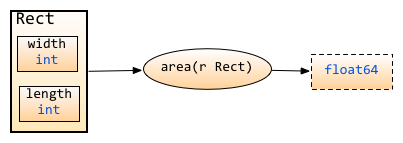
\includegraphics[width=8cm]{2.5.rect_func_without_receiver.png}
   \label{図2.8}
   \caption{メソッドとstructの関係図}
\end{figure}

明らかにこのような実現方法はエレガントではありません。それに概念からしても"面積"は"形状"の一属性です。これはある特定の形状に属しています。長方形の縦と横と同じようなものです。

このような理由から\texttt{method}の概念が生まれました。\texttt{method}はある型に属しています。この文法と関数の宣言の文法はほとんど同じです。ただ、\texttt{func}の後にreceiver(methodがくっついているということです)を追加します。

上で述べた形状の例からすると、method \texttt{area()} はある形状(たとえばRectangle)に由来して発生しています。Rectangle.area()の主語はRectangle、area()はRectangleに属するメソッドで外側の関数ではありません。

より具体的に述べると、Rectangleにはフィールドlengthとwidthが存在します。同時にarea()メソッドが存在します。これらのフィールドとメソッドは共にRectangleに属しています。

Rob Pikeの言葉を借りると:

\begin{quote}
"A method is a function with an implicit first argument, called a receiver."
\end{quote}

methodの文法は以下のとおりです:

\begin{lstlisting}[numbers=none]
func (r ReceiverType) funcName(parameters) (results)
\end{lstlisting}

はじめの例をとってmethodを実現してみます:

\begin{lstlisting}[numbers=none]
package main
import (
    "fmt"
    "math"
)

type Rectangle struct {
    width, height float64
}

type Circle struct {
    radius float64
}

func (r Rectangle) area() float64 {
    return r.width*r.height
}

func (c Circle) area() float64 {
    return c.radius * c.radius * math.Pi
}


func main() {
    r1 := Rectangle{12, 2}
    r2 := Rectangle{9, 4}
    c1 := Circle{10}
    c2 := Circle{25}

    fmt.Println("Area of r1 is: ", r1.area())
    fmt.Println("Area of r2 is: ", r2.area())
    fmt.Println("Area of c1 is: ", c1.area())
    fmt.Println("Area of c2 is: ", c2.area())
}
\end{lstlisting}

methodを使う時にはいくつか注意が必要です。

\begin{itemize}
  \item methodはまったく同じ名前でもレシーバが異なればmethodも異なります。
  \item methodはレシーバのフィールドにアクセスすることができます。
  \item methodの呼び出しは\texttt{.}を通じて行います。structがフィールドにアクセスするのと同じです。
\end{itemize}

図解:

\begin{figure}[H]
  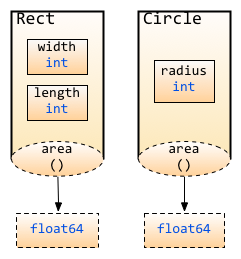
\includegraphics[width=6cm]{2.5.shapes_func_with_receiver_cp.png}
   \label{図2.9}
   \caption{異なるstructのmethodは異なる。}
\end{figure}

上の例では method area() はそれぞれRectangleとCircleに属します。この時これらの Receiver は Rectangle と Circleになります。またはこのarea()メソッドはRectangle/Circleを主語とします。

\begin{quote}
特に、図中のmethodは破線で表示しています。これは、このメソッドのレシーバは値渡しであり、参照渡しではありません。そうです。レシーバはポインタでもいいのです。両者の違いはポインタはレシーバがエンティティの内容に操作を行うことがあるのに対し、普通の型ではレシーバは操作するオブジェクトのコピーでしかありません。オリジナルのエンティティに対して操作が発生しないのです。詳細は後述します。
\end{quote}

methodはstructの上でしか使用されないのでしょうか?当然違います。これはカスタム定義型、ビルトイン型、structなどあらゆる型でも定義することができます。ちょっとよくわからなくなってきましたか?何がカスタム定義型だ、カスタム定義型はstructじゃないのか。そういうわけではありません。structはカスタム定義型のなかでも比較的特殊な型であるだけです。下のような宣言で実現します。

\begin{lstlisting}[numbers=none]
type typeName typeLiteral
\end{lstlisting}

以下のカスタム定義型の宣言のコードをご覧ください。

\begin{lstlisting}[numbers=none]
type ages int

type money float32

type months map[string]int

m := months {
    "January":31,
    "February":28,
    ...
    "December":31,
}
\end{lstlisting}

わかりましたか?簡単でしょう?このように自分のコードの中に意味のある型を定義することができるのです。実際はエイリアスを定義しているだけです。Cのtypedefに似たようなもので、例えば上のagesはintの代わりになっています。

それじゃあ、\texttt{method}にもどりましょう。

カスタム定義型の中で任意の\texttt{method}を定義することができます。次にちょっと複雑な例を見てみましょう。

\begin{lstlisting}[numbers=none]
package main
import "fmt"

const(
    WHITE = iota
    BLACK
    BLUE
    RED
    YELLOW
)

type Color byte

type Box struct {
    width, height, depth float64
    color Color
}

type BoxList []Box //a slice of boxes

func (b Box) Volume() float64 {
    return b.width * b.height * b.depth
}

func (b *Box) SetColor(c Color) {
    b.color = c
}

func (bl BoxList) BiggestColor() Color {
    v := 0.00
    k := Color(WHITE)
    for _, b := range bl {
        if bv := b.Volume(); bv > v {
            v = bv
            k = b.color
        }
    }
    return k
}

func (bl BoxList) PaintItBlack() {
    for i, _ := range bl {
        bl[i].SetColor(BLACK)
    }
}

func (c Color) String() string {
    strings := []string {"WHITE", "BLACK",
                         "BLUE", "RED", "YELLOW"}
    return strings[c]
}

func main() {
    boxes := BoxList {
        Box{4, 4, 4, RED},
        Box{10, 10, 1, YELLOW},
        Box{1, 1, 20, BLACK},
        Box{10, 10, 1, BLUE},
        Box{10, 30, 1, WHITE},
        Box{20, 20, 20, YELLOW},
    }

    fmt.Printf("We have %d boxes in our set\n",
               len(boxes))
    fmt.Println("The volume of the first one is",
                boxes[0].Volume(), "cm³")
    fmt.Println("The color of the last one is",
                boxes[len(boxes)-1].color.String())
    fmt.Println("The biggest one is",
                boxes.BiggestColor().String())

    fmt.Println("Let's paint them all black")
                boxes.PaintItBlack()
    fmt.Println("The color of the second one is",
                 boxes[1].color.String())

    fmt.Println("Obviously, now, the biggest one is",
                boxes.BiggestColor().String())
}
\end{lstlisting}

上のコードはconstでいくつかの定数を定義しています。その後カスタム定義型を定義しています。

\begin{itemize}
  \item Colorはbyteのエイリアスです。
  \item struct:Boxを定義します。3つの縦横高さのフィールドと色プロパティを持っています。
  \item slice:BoxListを定義します。Boxを持っています。
\end{itemize}

次に上のカスタム定義型をレシーバとしてmethodを定義します。

\begin{itemize}
  \item Volume()はレシーバをBoxとして定義します。Boxの体積を返します。
  \item SetColor(c Color)はBoxの色をcに変更します。
  \item BiggestColor()はBoxListに定義されており、listの中の体積が最大の色を返します。
  \item PaintItBlack()はBoxListのすべてのBoxの色を全部黒に変更します。
  \item String()はColorに定義されており、Colorの具体的な色を返します(文字列形式)
\end{itemize}

上のコードは文字で書くと非常に簡単に思えませんか?私達は問題を解決する場合問題の描写を通して、対応するコードを書くことで実現します。



\subsubsection{ポインタとしてのreceiver}
ではここで、SetColorのメソッドを見なおしてみましょう。このreceiverはBoxのポインタをさしています。そうです。*Boxを使えるのです。どうしてBox本体ではなくポインタを使うのでしょうか?

SetColorを定義した本当の目的はこのBoxの色を変更することです。もしBoxのポインタを渡さなければ、SetColorが受け取るのは実はBoxのコピーになってしまいます。つまり、メソッド内で色の変更を行うと、Boxのコピーを操作しているだけで、本当のBoxではないのです。そのため、ポインタを渡す必要があります。

ここではreceiverをメソッドの第一引数にしました。こうすれば前の関数で説明した値渡しと参照渡しも難しくなくなるでしょう。

もしかしたらSetColor関数の中で以下のように定義すべきじゃないかと思われたかもしれません。\texttt{*b.Color=c}、ところが\texttt{b.Color=c}でよいのです。ポインタに対応する値を読み込むことが必要ですから。

そのとおりです。Goの中ではこの2つの方法はどちらも正しいのです。ポインタを使って対応するフィールドにアクセスした場合(ポインタになんのフィールドがなかったとしても)、Goはあなたがポインタを通してその値を必要としていることを知っています。どうです。Goのデザインに魅了されてきたんじゃないですか?

注意深い読者はこのように思うかもしれません。PointItBlackの中でSetColorをコールした時、ひょっとして\texttt{(\&bl[i]).SetColor(BLACK)}と書かなければならないんじゃないかと。SetColorのreceiverは*Boxであり、Boxではありませんから。

ええ、その通りなんです。この2つの方法はどちらでもかまいません。Goはreceiverがポインタであることを知っています。こいつは自動的に解釈してくれるのです。

つまり:

\begin{quote}
もしメソッドのreceiverが*Tであれば、T型のエンティティの変数V上でこのメソッドをコールすることができます。\&Vによってメソッドをコールする必要はありません。
\end{quote}



\begin{quote}
もしメソッドのreceiverがTであれば、T型の変数P上でこのメソッドをコールすることができます。Pを使ってメソッドをコールする必要はありません。
\end{quote}

ですので、コールしているポインタのメソッドがポインタのメソッドであるかどうかは気にする必要がありません。Goはあなたが行おうとしているすべてのことを知っているのです。C/C++でプログラムを経験されてこられた方にとっては、とてもとても大きな苦痛が解決されることでしょう。

\subsubsection{method継承}
前の章でフィールドの継承を学びました。するとあなたはGoの不思議なところに気がついたかもしれません。methodも継承できるのです。もし匿名フィールドが一つのメソッドを実現している場合、この匿名フィールドを含むsturctもこのメソッドをコールすることができるのです。例をお見せします。


\begin{lstlisting}[numbers=none]
  package main
  import "fmt"

  type Human struct {
    name string
    age int
    phone string
  }

  type Student struct {
    Human //匿名フィールド
    school string
  }

  type Employee struct {
    Human //匿名フィールド
    company string
  }

  //human上でメソッドを定義
  func (h *Human) SayHi() {
    fmt.Printf("Hi, I am %s you can call me on %s\n",
               h.name, h.phone)
  }

  func main() {
    mark := Student{Human{"Mark", 25, "222-222-YYYY"},
                    "MIT"}
    sam := Employee{Human{"Sam", 45, "111-888-XXXX"},
                    "Golang Inc"}

    mark.SayHi()
    sam.SayHi()
  }
\end{lstlisting}

\subsubsection{methodの書き直し}
上の例で、もしEmployeeにSayHiを実現したい場合はどうすればよいでしょうか?簡単です。匿名フィールドの衝突と同じ道理で、Employee上でもメソッドを定義することができます。匿名フィールドを書き直す方法は下の例をご確認ください。

\begin{lstlisting}[numbers=none]
package main
import "fmt"

type Human struct {
    name string
    age int
    phone string
}

type Student struct {
    Human //匿名フィールド
    school string
}

type Employee struct {
    Human //匿名フィールド
    company string
}

//Humanでmethodを定義
func (h *Human) SayHi() {
    fmt.Printf("Hi, I am %s you can call me on %s\n",
               h.name, h.phone)
}

//EmployeeのmethodでHumanのmethodを書き直す。
func (e *Employee) SayHi() {
  fmt.Printf("Hi, I am %s, I work at %s. Call me on %s\n",
             e.name, e.company, e.phone)
            //Yes you can split into 2 lines here.
}

func main() {
    mark := Student{Human{"Mark", 25, "222-222-YYYY"},
                   "MIT"}
    sam := Employee{Human{"Sam", 45, "111-888-XXXX"},
                  "Golang Inc"}

    mark.SayHi()
    sam.SayHi()
}
\end{lstlisting}

上のコードのデザインはこのように絶妙です。Goのデザインに驚くことでしょう。

このように、基本的なオブジェクト指向のプログラムを設計することができます。ですが、Goのオブジェクト指向はこのように簡単です。プライベートやパブリックといったキーワードは出てきません。大文字と小文字によって実現しているのです(大文字で始まるものはパブリック、小文字で始まるものはプライベートです)、メソッドにも同じルールが適用されます。



\subsection{interface}
\subsubsection{interface}
Goではとても繊細なinterfaceと呼ぶべき設計があります。これはオブジェクト指向と内容構成にとって非常に便利です。この章を終わった時にはあなたはinterfaceの巧妙な設計に感服することでしょう。


\subsubsection{interfaceとは何か}
簡単にいえば、interfaceはmethodの組み合わせです。interfaceを通してオブジェクトの振る舞いを定義することができます。

前の章の最後の例でStudentとEmployeeはどちらもSayHiを持っていました。彼らの内部処理は異なりますが、それは重要ではありません。重要なのは彼らがどちらも\texttt{say hi}と言えることです。

続けてさらに拡張していきましょう。StudentとEmployeeで他のメソッド\texttt{Sing}を実現します。その後StudentはBorrowMoneyメソッドを追加してEmployeeはSpendSalaryを追加しましょう。

Studentには3つのメソッドがあることになります:SayHi、Sing、BorrowMoneyです。EmployeeはSayHi、Sing、SpendSalaryです。

このようなメソッドの組み合わせはinterfaceと呼ばれます。そして、それらはStudentとEmployeeで実装されます。StudentとEmployeeはinterfaceのSayHiとSingを実装します。同時にEmployeeはBorrowMoneyを実装しません。そして、StudentはSpendSalaryを実装しません。なぜなら、EmployeeはBorrowMoneyメソッドを持っていません。また、StudentはSpendSalaryメソッドを持っていないからです。


\subsubsection{interface型}
interface型ではメソッドのセットを定義します。もしあるオブジェクトがインターフェースとなるすべてのメソッドを実装するとしたら、このオブジェクトはこのインターフェースを実装することになります。細かい文法は下の例を参考にしてください。

\begin{lstlisting}[numbers=none]
type Human struct {
    name string
    age int
    phone string
}

type Student struct {
    Human //匿名フィールドHuman
    school string
    loan float32
}

type Employee struct {
    Human //匿名フィールドHuman
    company string
    money float32
}

//HumanオブジェクトにSayHiメソッドを実装します。
func (h *Human) SayHi() {
    fmt.Printf("Hi, I am %s you can call me on %s\n",
               h.name, h.phone)
}

// HumanオブジェクトにSingメソッドを実装します。
func (h *Human) Sing(lyrics string) {
    fmt.Println("La la, la la la, la la la la la...",
                lyrics)
}

//HumanメソッドにGuzzleメソッドを実装します。
func (h *Human) Guzzle(beerStein string) {
    fmt.Println("Guzzle Guzzle Guzzle...", beerStein)
}

// EmployeeはHumanのSayHiメソッドをオーバーロードします。
func (e *Employee) SayHi() {
    fmt.Printf("Hi, I am %s, I work at %s. Call me on %s\n",
               e.name, e.company, e.phone)
              //この行は複数に渡ってもかまいません。
}

//StudentはBorrowMoneyメソッドを実装します。
func (s *Student) BorrowMoney(amount float32) {
    s.loan += amount // (again and again and...)
}

//EmployeeはSpendSalaryメソッドを実装します。
func (e *Employee) SpendSalary(amount float32) {
    e.money -= amount
    // More vodka please!!! Get me through the day!
}

// interfaceを定義します。
type Men interface {
    SayHi()
    Sing(lyrics string)
    Guzzle(beerStein string)
}

type YoungChap interface {
    SayHi()
    Sing(song string)
    BorrowMoney(amount float32)
}

type ElderlyGent interface {
    SayHi()
    Sing(song string)
    SpendSalary(amount float32)
}
\end{lstlisting}

上のコードを通して、interfaceは任意のオブジェクトで実装できることがわかるかと思います。上のMen interfaceはHuman、Student及びEmployeeによって実装されます。例えばStudentはMenとYoungChapの2つのinterfaceを実装することになります。

最後に、任意の型は空のinterface(ここではinterface\{\}と定義しましょう)を実装しています。これには0個のメソッドが含まれるinterfaceです。

\subsubsection{interfaceの値}
では、interfaceの中には一体どのような値が存在しているのでしょうか。もし我々がinterfaceの変数を定義すると、この変数にはこのinterfaceの任意の型のオブジェクトを保存することができます。上の例でいえば、我々はMen interface型の変数mを定義しました。このmにはHuman、StudentまたはEmployeeの値を保存できます。

mは3つの型を持つことのできるオブジェクトなので、Men型の要素を含むsliceを定義することができます。このsliceはMenインターフェースの任意の構造のオブジェクトを代入することができます。このsliceともともとのsliceにはいくつか違いがあります。

次の例を見てみましょう。

\begin{lstlisting}[numbers=none]
package main
import "fmt"

type Human struct {
    name string
    age int
    phone string
}

type Student struct {
    Human //匿名フィールド
    school string
    loan float32
}

type Employee struct {
    Human //匿名フィールド
    company string
    money float32
}

//HumanにSayHiメソッドを実装します。
func (h Human) SayHi() {
    fmt.Printf("Hi, I am %s you can call me on %s\n",
               h.name, h.phone)
}

//HumanにSingメソッドを実装します。
func (h Human) Sing(lyrics string) {
    fmt.Println("La la la la...", lyrics)
}

//EmployeeはHumanのSayHiメソッドをオーバーロードします。
func (e Employee) SayHi() {
    fmt.Printf("Hi, I am %s, I work at %s. Call me on %s\n",
               e.name, e.company, e.phone)
    }

// Interface MenはHuman,StudentおよびEmployeeに実装されます。
// この3つの型はこの2つのメソッドを実装するからです。
type Men interface {
    SayHi()
    Sing(lyrics string)
}

func main() {
    mike := Student{Human{"Mike", 25, "222-222-XXX"},
                    "MIT", 0.00}
    paul := Student{Human{"Paul", 26, "111-222-XXX"},
                   "Harvard", 100}
    sam := Employee{Human{"Sam", 36, "444-222-XXX"},
                    "Golang Inc.", 1000}
    tom := Employee{Human{"Tom", 37, "222-444-XXX"},
                    "Things Ltd.", 5000}

    //Men型の変数iを定義します。
    var i Men

    //iにはStudentを保存できます。
    i = mike
    fmt.Println("This is Mike, a Student:")
    i.SayHi()
    i.Sing("November rain")

    //iにはEmployeeを保存することもできます。
    i = tom
    fmt.Println("This is Tom, an Employee:")
    i.SayHi()
    i.Sing("Born to be wild")

    //sliceのMenを定義します。
    fmt.Println("Let's use a slice of Men and see what happens")
    x := make([]Men, 3)
    //この3つはどれも異なる要素ですが、
    //同じインターフェースを実装しています。
    x[0], x[1], x[2] = paul, sam, mike

    for _, value := range x{
        value.SayHi()
    }
}
\end{lstlisting}

上のコードで、interfaceはメソッドの集合を抽象化したものだとお分かりいただけるとおもいます。他のinterfaceでない型によって実装されなければならず、自分自身では実装することができません。Goはinterfaceを通してduck-typingを実現できます。すなわち、"鳥の走る様子も泳ぐ様子も鳴く声もカモのようであれば、この鳥をカモであると呼ぶことができる"わけです。

\subsubsection{空のinterface}
空のinterface(interface\{\})にはなんのメソッドも含まれていません。この通り、すべての型は空のinterfaceを実装しています。空のinterfaceはそれ自体はなんの意味もありません(何のメソッドも含まれていませんから)が、任意の型の数値を保存する際にはかなり役にたちます。これはあらゆる型の数値を保存することができるため、C言語のvoid*型に似ています。

\begin{lstlisting}[numbers=none]
// aを空のインターフェースとして定義
var a interface{}
var i int = 5
s := "Hello world"
// aは任意の型の数値を保存できます。
a = i
a = s
\end{lstlisting}

ある関数がinterface\{\}を引数にとると、任意の型の値を引数にとることができます。もし関数がinterface\{\}を返せば、任意の型の値を返すことができるのです。とても便利ですね!

\subsubsection{interface関数の引数}
interfaceの変数はこのinterface型のオブジェクトを持つことができます。これにより、関数(メソッドを含む)を書く場合思いもよらない思考を与えてくれます。interface引数を定義することで、関数にあらゆる型の引数を受けさせることができるです。

例をあげましょう:fmt.Printlnは私達がもっともよく使う関数です。ですが、任意の型のデータを受けることができる点に気づきましたか。fmtのソースファイルを開くとこのような定義が書かれています:


\begin{lstlisting}[numbers=none]
type Stringer interface {
     String() string
}
\end{lstlisting}

つまり、Stringメソッドを持つ全ての型がfmt.Printlnによってコールされることができるのです。ためしてみましょう。

\begin{lstlisting}[numbers=none]
package main
import (
    "fmt"
    "strconv"
)

type Human struct {
    name string
    age int
    phone string
}

// このメソッドを使ってHumanにfmt.Stringerを実装します。
func (h Human) String() string {
    return "<"+h.name+" - "+strconv.Itoa(h.age)+
           " years -  Tel:" +h.phone+">"
}

func main() {
    Bob := Human{"Bob", 39, "000-7777-XXX"}
    fmt.Println("This Human is : ", Bob)
}
\end{lstlisting}

前のBoxの例を思い出してみましょう。Color構造体もメソッドを一つ定義しています:String。実はこれもfmt.Stringerというinterfaceを実装しているのです。つまり、もしある型をfmtパッケージで特殊な形式で出力させようとした場合Stringerインターフェースを実装する必要があります。もしこのインターフェースを実装していなければ、fmtはデフォルトの方法で出力を行います。

\begin{lstlisting}[numbers=none]
//同じ機能を実装します。
fmt.Println("The biggest one is",
            boxes.BiggestsColor().String())
fmt.Println("The biggest one is",
            boxes.BiggestsColor())
\end{lstlisting}

注:errorインターフェースのオブジェクト(Error() stringのオブジェクトを実装)を実装します。fmtを使って出力を行う場合、Error()メソッドがコールされます。そのため、String()メソッドを再定義する必要はありません。

\subsubsection{interface変数を保存する型}
interfaceの変数の中にはあらゆる型の数値を保存できることを学びました(この型はinterfaceを実装しています)。では、この変数に実際に保存されているのはどの型のオブジェクトであるかどのように逆に知ることができるのでしょうか?現在二種類の方法があります:

\paragraph{Comma-okアサーション}

 Go言語の文法では、ある変数がどの型か直接判断する方法があります: value, ok = element.(T), ここでvalueは変数の値を指しています。okはbool型です。elementはinterface変数です。Tはアサーションの型です。

もしelementにT型の数値が存在していれば、okにはtrueが返されます。さもなければfalseが返ります。

例を見ながら詳しく理解していきましょう。

\begin{lstlisting}[numbers=none]
package main

import (
    "fmt"
    "strconv"
)

type Element interface{}
type List [] Element

type Person struct {
    name string
    age int
}

//Stringメソッドを定義します。fmt.Stringerを実装します。
func (p Person) String() string {
    return "(name: " + p.name + " - age: "
           +strconv.Itoa(p.age)+ " years)"
}

func main() {
    list := make(List, 3)
    list[0] = 1 // an int
    list[1] = "Hello" // a string
    list[2] = Person{"Dennis", 70}

    for index, element := range list {
        if value, ok := element.(int); ok {
            fmt.Printf("list[%d] is an int and its value is %d\n",
                       index, value)
        } else if value, ok := element.(string); ok {
            fmt.Printf("list[%d] is a string and its value is %s\n",
                       index, value)
        } else if value, ok := element.(Person); ok {
            fmt.Printf("list[%d] is a Person and its value is %s\n",
                       index, value)
        } else {
            fmt.Printf("list[%d] is of a different type\n", index)
        }
    }
}
\end{lstlisting}

 とても簡単ですね。前のフローの項目の際にご紹介したとおり、いくつもifの中で変数の初期化が許されているのにお気づきでしょうか。

また、アサーションの型が増えれば増えるほど、ifelseの数も増えるのにお気づきかもしれません。下ではswitchをご紹介します。

\paragraph{switchテスト}

コードの例をお見せしたほうが早いでしょう。上の実装をもう一度書きなおしてみます。

\begin{lstlisting}[numbers=none]
package main

import (
    "fmt"
    "strconv"
)

type Element interface{}
type List [] Element

type Person struct {
    name string
    age int
}

//プリント
func (p Person) String() string {
    return "(name: " + p.name + " - age: "
           +strconv.Itoa(p.age)+ " years)"
}

func main() {
    list := make(List, 3)
    list[0] = 1 //an int
    list[1] = "Hello" //a string
    list[2] = Person{"Dennis", 70}

    for index, element := range list{
        switch value := element.(type) {
            case int:
              fmt.Printf("list[%d] is an int and its value is %d\n",
                         index, value)
            case string:
              fmt.Printf("list[%d] is a string and its value is %s\n",
                         index, value)
            case Person:
              fmt.Printf("list[%d] is a Person and its value is %s\n",
                         index, value)
            default:
              fmt.Println("list[%d] is of a different type",
                          index)
        }
    }
}
\end{lstlisting}

ここで強調したいのは、\texttt{element.(type)}という文法はswitchの外のロジックで使用できないということです。もしswitchの外で型を判断したい場合は\texttt{comma-ok}を使ってください。

\subsubsection{組み込みinterface}
Goが本当に魅力的なのはビルトインのロジック文法です。Structを学んだ際の匿名フィールドはあんなにもエレガントでした。では同じようなロジックをinterfaceに導入すればより完璧になります。もしinterface1がinterface2の組み込みフィールドであれば、interface2は暗黙的にinterface1のメソッドを含むことになります。

ソースパッケージのcontainer/heapの中にこのような定義があるのを確認できると思います。

\begin{lstlisting}[numbers=none]
type Interface interface {
    sort.Interface
    //組み込みフィールドsort.Interface
    Push(x interface{})
    //a Push method to push elements into the heap
    Pop() interface{}
    //a Pop elements that pops elements from the heap
}
\end{lstlisting}

sort.Interfaceは実は組み込みフィールドです。sort.Interfaceのすべてのメソッドを暗黙的に含んでいます。つまり以下の3つのメソッドです。

\begin{lstlisting}[numbers=none]
type Interface interface {
    // Len is the number of elements in the collection.
    Len() int
    // Less returns whether the element with index i should sort
    // before the element with index j.
    Less(i, j int) bool
    // Swap swaps the elements with indexes i and j.
    Swap(i, j int)
}
\end{lstlisting}

もう一つの例はioパッケージの中にある io.ReadWriterです。この中にはioパッケージのReaderとWriterの2つのinterfaceを含んでいます:

\begin{lstlisting}[numbers=none]
// io.ReadWriter
type ReadWriter interface {
    Reader
    Writer
}
\end{lstlisting}


\subsubsection{リフレクション}
Goはリフレクションを実装しています。リフレクションはプログラムの実行時の状態を検査することができます。私達が一般的に使用しているパッケージはreflectパッケージです。どのようにreflectパッケージを使うかはオフィシャルのドキュメントに詳細な原理が説明されています。laws of reflection(http:\//\//golang.org\//doc\//articles\//laws\_of\_reflection.html)

reflectを使うには3つのステップに分けられます。下で簡単にご説明します:リフレクションは型の値(これらの値はすべて空のインターフェースを実装しています。)。まずこれをreflectオブジェクトに変換する必要があります(reflect.Typeまたはreflect.Valueです。異なる状況によって異なる関数をコールします。)この2つを取得する方法は:

\begin{lstlisting}[numbers=none]
t := reflect.TypeOf(i)
//元データを取得します。tを通して型定義の中の
//すべての要素を取得することができます。
v := reflect.ValueOf(i)
//実際の値を取得します。vを通して保存されている
//中の値を取得することができます。値を変更することもできます。
\end{lstlisting}

reflectオブジェクトに変換した後、何かしらの操作を行うことができます。つまり、reflectオブジェクトを対応する値に変換するのです。例えば

\begin{lstlisting}[numbers=none]
tag := t.Elem().Field(0).Tag
//structの中で定義されているタグを取得する。
name := v.Elem().Field(0).String()
//はじめのフィールドに保存されている値を取得する。
\end{lstlisting}

reflectの値を取得することで対応する型と数値を返すことができます。

\begin{lstlisting}[numbers=none]
var x float64 = 3.4
v := reflect.ValueOf(x)
fmt.Println("type:", v.Type())
fmt.Println("kind is float64:", v.Kind() == reflect.Float64)
fmt.Println("value:", v.Float())
\end{lstlisting}

最後にリフレクションを行ったフィールドは修正できる必要があります。前で学んだ値渡しと参照渡しも同じ道理です。リフレクションのフィールドが必ず読み書きできるということは、以下のように書いた場合、エラーが発生するということです。



\begin{lstlisting}[numbers=none]
var x float64 = 3.4
v := reflect.ValueOf(x)
v.SetFloat(7.1)
\end{lstlisting}

もし対応する値を変更したい場合、このように書かなければなりません。

\begin{lstlisting}[numbers=none]
var x float64 = 3.4
p := reflect.ValueOf(&x)
v := p.Elem()
v.SetFloat(7.1)
\end{lstlisting}

上はリフレクションに対する簡単なご説明ではありますが、より深い理解には実際のプログラミングで実践していく他ありません。


\subsection{マルチスレッド}
Goを21世紀のC言語だという人もいます。Go言語は設計が簡単で、21世紀で最も重要なのはマルチスレッドだからです。Goは言語レベルでマルチスレッドをサポートしています。

\subsubsection{goroutine}
goroutineはGoのマルチスレッドのコアです。goroutineは実は最初から最後までスレッドです。しかしスレッドよりも小さく、十数個のgoroutineは低レイヤーで5,6個のスレッドを実現しているだけです。Go言語の内部ではこれらのgoroutineの間ではメモリの共有を実現しています。goroutineを実行するには非常に少ないスタックメモリ(大体4$\sim$5KBです。)を必要とするだけです。当然対応するデータによって伸縮しますが、まさにこのためいくつものマルチスレッドタスクを実行することができます。goroutineはthreadに比べより使いやすく、効果的で、便利です。

goroutineはGoのruntime管理を利用したスレッドコントローラです。goroutineは\texttt{go}キーワードによって実現します。実は単なる普通の関数です。

\begin{lstlisting}[numbers=none]
go hello(a, b, c)
\end{lstlisting}

キーワードgoを通じてgoroutineを起動します。例を見てみましょう。

\begin{lstlisting}[numbers=none]
package main

import (
    "fmt"
    "runtime"
)

func say(s string) {
    for i := 0; i < 5; i++ {
        runtime.Gosched()
        fmt.Println(s)
    }
}

func main() {
    go say("world") //新しいGoroutinesを実行する。
    say("hello") //現在のGoroutines実行
}

// 上のプログラムを実行すると以下のように出力されます:
// hello
// world
// hello
// world
// hello
// world
// hello
// world
// hello
\end{lstlisting}

goキーワードで非常に簡単にマルチスレッドプログラミングを実現することがお分かりいただけるかと思います。 上の複数のgoroutineは同じプロセスで実行されています。メモリのデータを共有しますが、デザイン上共有を利用して通信を行ったりせず、通信によって共有を行うようにしましょう。


\begin{quote}
    runtime.Gosched()ではCPUに時間を他の人に受け渡します。次にある段階で継続してこのgoroutineを実行します。

    デフォルトでは、ディスパッチャはプロセスを使うのみで、マルチスレッドを実現するだけです。マルチコアプロセッサのマルチスレッドを実現したい場合は、我々のプログラムでruntime.GOMAXPROCS(n)をコールすることでディスパッチャに同時に複数のプロセスを使用させる必要があります。GOMAXPROCSは同時に実行するロジックコードのシステムプロセスの最大数を設定し、前の設定を返します。もしn < 1であった場合、現在の設定は変更されません。Goの新しいバージョンでディスパッチャが修正されれば、これは削除されるでしょう。Robによるマルチスレッドの開発についてはこちらに文章があります。http:\//\//concur.rspace.googlecode.com\//hg\//talk\//concur.html\#landing-slide
\end{quote}



\subsubsection{channels}
goroutineは同じアドレス空間で実行されます。そのため、共有されたメモリへのアクセスはかならず同期されていなければなりません。では、goroutineの間ではどのようにしてデータの通信を行うのでしょうか。Goはチャネルというとても良い通信機構を提供しています。チャネルはUnix shellとの双方向パイプを作成します。これを通して値を送信したり受信することができます。これらの値は特定の型のみが許容されます。チャネル型。channelを定義した場合チャネルに送信する値の型も定義しなければなりません。ご注意ください。かならずmakeを使ってchannelを作成します。

\begin{lstlisting}[numbers=none]
ci := make(chan int)
cs := make(chan string)
cf := make(chan interface{})
\end{lstlisting}

channelは\texttt{<-}演算子を使ってデータを送ったり受けたりします。

\begin{lstlisting}[numbers=none]
ch <- v    // vをchannel chに送る。
v := <-ch  // chの中からデータを受け取り、vに代入する。
\end{lstlisting}

これを私達の例の中に当てはめてみましょう:

\begin{lstlisting}[numbers=none]
package main

import "fmt"

func sum(a []int, c chan int) {
    total := 0
    for _, v := range a {
        total += v
    }
    c <- total  // send total to c
}

func main() {
    a := []int{7, 2, 8, -9, 4, 0}

    c := make(chan int)
    go sum(a[:len(a)/2], c)
    go sum(a[len(a)/2:], c)
    x, y := <-c, <-c  // receive from c

    fmt.Println(x, y, x + y)
}
\end{lstlisting}

デフォルトでは、channelがやり取りするデータはブロックされています。もう片方が準備できていなければ、Goroutinesの同期はもっと簡単になります。lockを表示する必要はありません。いわゆるブロックとは、もし(value := $<$-ch)を読み取った場合、これはブロックされます。データを受け取った段階で(ch$<$-5)を送信するいずれのものもデータが読み込まれるまでブロックされます。バッファリングの無いchannelは複数のgoroutineの間で同期を行う非常に優れたツールです。



\subsubsection{Buffered Channels}
上ではデフォルトでバッファリング型の無いchannelをご紹介しました。しかし、Goはchannelのバッファリングの大小も指定することを許しています。とても簡単です。つまりchannelはいくつもの要素を保存することができるのです。ch:= make(chan bool, 4)は4つのbool型の要素を持てるchannelを作成します。このchannelの中で、前の4つの要素はブロックされずに入力することができます。5番目の要素が入力された場合、コードはブロックされ、その他のgoroutineがchannelから要素を取り出すまで空間を退避します。


\begin{lstlisting}[numbers=none]
ch := make(chan type, value)

value == 0 ! バッファリング無し(ブロック)
value > 0 ! バッファリング(ブロック無し、value個の要素まで)
\end{lstlisting}

下の例をご覧ください。ローカルでテストしてみることができます。対応するvalue値を変更してください

\begin{lstlisting}[numbers=none]
package main

import "fmt"

func main() {
    c := make(chan int, 2)
    //2を1に修正するとエラーが発生します。
    //2を3に修正すると正常に実行されます。
    c <- 1
    c <- 2
    fmt.Println(<-c)
    fmt.Println(<-c)
}
\end{lstlisting}


\subsubsection{RangeとClose}
上の例では、2回cの値を読み込む必要がありました。これではあまり便利ではありません。Goはこの点を考慮し、rangeによってsliceやmapを操作するのと同じ感覚でバッファリング型のchannelを操作することができます。下の例をご覧ください。


\begin{lstlisting}[numbers=none]
package main

import (
    "fmt"
)

func fibonacci(n int, c chan int) {
    x, y := 1, 1
    for i := 0; i < n; i++ {
        c <- x
        x, y = y, x + y
    }
    close(c)
}

func main() {
    c := make(chan int, 10)
    go fibonacci(cap(c), c)
    for i := range c {
        fmt.Println(i)
    }
}
\end{lstlisting}

\texttt{for i := range c}でこのchannelがクローズを明示されるまで連続してchannelの中のデータを読み込むことができます。上のコードでchannelのクローズが明示されているのが確認できるかと思います。生産者は\texttt{close}ビルトイン関数によってchannelを閉じます。channelを閉じた後はいかなるデータも送信することはできません。消費側は\texttt{v, ok := <-ch}という式でchannelがすでに閉じられているかテストすることができます。もしokにfalseが返ってきたら、channelはすでにどのようなデータも無く、閉じられているということになります。

\begin{quote}
生産者の方でchannelが閉じられる事に注意してください。消費側ではありません。これは容易にpanicを引き起こします。

また、channelはファイルのようなものでないことにも注意してください。頻繁に閉じる必要はありません。何のデータも送ることが無い場合またはrangeループを終了させたい場合などで結構です。
\end{quote}

\subsubsection{Select}
ここではひとつだけのchannelがある状況についてご紹介しました。では複数のchannelが存在した場合、どのように操作すべきでしょうか。Goではキーワード\texttt{select}を提供しています。\texttt{select}を通して、channel上のデータを監視することができます。

\texttt{select}はデフォルトでブロックされます。channelの中でやりとりされるデータを監視する時のみ実行します。複数のchannelの準備が整った時に、selectはランダムにひとつ選択し、実行します。

\begin{lstlisting}[numbers=none]
package main

import "fmt"

func fibonacci(c, quit chan int) {
    x, y := 1, 1
    for {
        select {
        case c <- x:
            x, y = y, x + y
        case <-quit:
            fmt.Println("quit")
            return
        }
    }
}

func main() {
    c := make(chan int)
    quit := make(chan int)
    go func() {
        for i := 0; i < 10; i++ {
            fmt.Println(<-c)
        }
        quit <- 0
    }()
    fibonacci(c, quit)
}
\end{lstlisting}

\texttt{select}の中にもdefault文があります。\texttt{select}は実はswitchの機能によくにています。defaultは監視しているchannelがどれも準備が整っていない時に、デフォルトで実行されます。(selectはchannelを待ってブロックしません。)

\begin{lstlisting}[numbers=none]
select {
case i := <-c:
    // use i
default:
    // cがブロックされた時にここが実行されます。
}
\end{lstlisting}


\subsubsection{タイムアウト}
ときどきgoroutineがブロックされる状況にでくわします。ではプログラム全体がブロックされる状況をどのように回避するのでしょうか?selectを使ってタイムアウトを設定することができます。下のような方法で実現します:

\begin{lstlisting}[numbers=none]
func main() {
    c := make(chan int)
    o := make(chan bool)
    go func() {
        for {
            select {
                case v := <- c:
                    println(v)
                case <- time.After(5 * time.Second):
                    println("timeout")
                    o <- true
                    break
            }
        }
    }()
    <- o
}
\end{lstlisting}

\subsubsection{runtime goroutine}
runtimeパッケージにはgoroutineを処理するいくつかの関数が含まれます:

\begin{description}
  \item[Goexit] 事前に実行されたgoroutineから抜けます。ただし、defer関数は継続してコールされます。
  \item[Gosched] 事前のgoroutineの実行権限をジェネレートします。ディスパッチャが他の待機中のタスクの実行を予定し、次のある時点でこの位置から実行を復元します。
  \item[NumCPU] CPUのコア数を返します。
  \item[NumGoroutine] 現在実行しているgoroutineの総数を返します。
  \item[GOMAXPROCS] 実行できるCPUコア数の最大値を設定し、前のコア数を返します。
\end{description}


\subsection{まとめ}
この章では主にGo言語のいくつかの文法をご紹介しました。文法を通してGoがいかに簡単かご覧いただけたかと思います。たった25個のキーワードです。もう一度これらキーワードが何に使われるのか見てみることにしましょう。

\begin{lstlisting}[numbers=none]
break    default      func    interface    select
case     defer        go      map          struct
chan     else         goto    package      switch
const    fallthrough  if      range        type
continue for          import  return       var
\end{lstlisting}


\begin{itemize}
  \item varとconstは2.2のGo言語の基礎に出てくる変数と定数の宣言を参考にしてください。
  \item packageとimportにはすでに少し触れました。
  \item func は関数とメソッドの定義に用いられます。
  \item return は関数から返るために用いられます。
  \item defer はデストラクタのようなものです。
  \item go はマルチスレッドに用いられます。
  \item select は異なる型の通信を選択するために用いられます。
  \item interface はインターフェースを定義するために用いられます。2.6章をご参考ください。
  \item struct は抽象データ型の定義に用いられます。2.5章をご参考ください。
  \item break、case、continue、for、fallthrough、else、if、switch、goto、defaultは2.3のフロー紹介をご参考ください。
  \item chanはchannel通信に用いられます。
  \item typeはカスタム定義型の宣言に用いられます。
  \item mapはmap型のデータの宣言に用いられます。
  \item rangeはslice、map、channelデータの読み込みに用いられます。
\end{itemize}




\section{Webの基礎}
Webのプログラミングの基礎を勉強することはあなたにとってまさにこの本を読む理由でしょう。事実、どのようにGoを使ってWebアプリケーションをプログラムするかはこの本の目的でもあります。前回までで、Goは既に成熟したHTTP処理パッケージを持つことをご紹介しました。これによってどのような事情の動的なWebプログラミングも簡単に作成できます。これ以降の章でご紹介する内容はどれもWebプログラミングの範疇です。この章ではWebに関する概念とGo言語がいかにWebプログラムを実行するかに集中して討論します。


\subsection{webでの作業方法}
普段ホームページを閲覧する際、ブラウザを開くと思います。アドレスを入力してエンターキーを押すと、あなたが見たいコンテンツが表示されます。この見た目には簡単なユーザの行動には一体何が隠されているのでしょうか?

普通のネットワーク上の操作に対して、システムは実はこのように行なっています:ブラウザそのものはクライアントです。URLを入力する際まずブラウザはDNSサーバにアクセスします。DNSを通してドメインと対応するIPを取得し、IPアドレスからIPに対応したサーバを探しだした後、TCPコネクションの設立を要求します。ブラウザがHTTP Request(リクエスト)パケットを送信し終わると、サーバはリクエストパケットを受け取ってリクエストパケットを処理しはじめます。サーバは自分のサービスをコールし、HTTP Response(レスポンス)パケットを返します。クライアントがサーバからのレスポンスを受け取ると、このレスポンスパケットのbodyを読み出します。すべての内容を受け取ると、このサーバとのTCP接続を切断します。


\begin{figure}[H]
  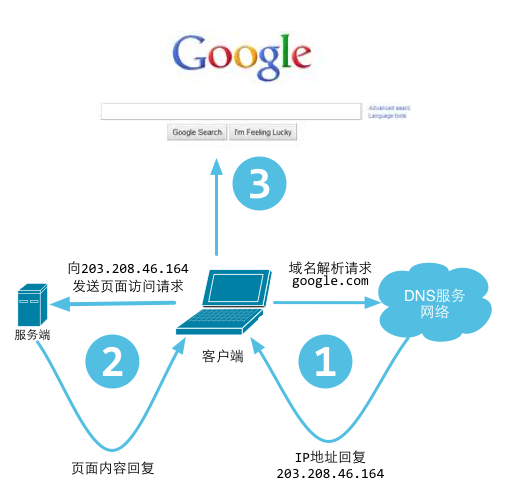
\includegraphics[width=14cm]{3.1.web2.png}
   \label{図3.1}
   \caption{ユーザがWebサーバにアクセスする過程}
\end{figure}


WebサーバはHTTPサーバとも呼ばれます。HTTPプロトコルを通じてクライアントと通信を行います。このクライアントは普通はWebブラウザを指します(実はモバイルクライアントでも内部ではブラウザによって実現されています。)

Webサーバの動作原理は簡単に説明できます:

\begin{itemize}
  \item クライアントがTCP/IPプロトコルによってサーバまでTCP接続を設立します。
  \item クライアントはサーバに対してHTTPプロトコルのリクエストパケットを送信し、サーバのリソースドキュメントを要求します。
  \item サーバはクライアントに対してHTTPプロトコルの応答パケットを送信し、もし要求されたリソースに動的な言語によるコンテンツが含まれている場合、サーバが動的言語のインタープリターエンジンに"動的な内容"の処理をコールさせます。処理によって得られたデータをクライアントに返します。
  \item クライアントとサーバが切断されます。クライアントはHTMLドキュメントを解釈し、クライアントの画面上に図形として結果を表示します。
\end{itemize}


簡単なHTTPタスクはこのように実現されます。見た目にはとても複雑ですが、原理はとても簡単です。気をつけなければならないのは、クライアントとサーバの間の通信は常に接続されているわけではありません。サーバが応答を送信した後クライアントと接続が切断され、次のリクエストを待ち受けます。

\subsubsection{URLとDNS解決}
ホームページの閲覧は常にURLの訪問で行われます。ではURLとは一体どういうものなのでしょうか?

URL(Uniform Resource Locator)は"統一資源位置指定子"の英語の短縮です。ネットワーク上のリソースを表現しています。基本的なシンタックスは以下のとおりです。

\begin{lstlisting}[numbers=none]
scheme://host[:port#]/path/.../[?query-string][#anchor]
scheme         低レイヤーで使用されるプロトコルを指定します。
              (例えば:http, https, ftp)
host           HTTPサーバのIPアドレスまたはドメイン
port#          HTTPサーバのデフォルトのポート番号は80です。
               この場合ポート番号は省略することができます。
               もし別のポートを使用する場合は指定しなければなりません。
               例えば http://www.cnblogs.com:8080/
path           リソースまでのパス
query-string   httpサーバへ送るデータ
anchor         アンカー
\end{lstlisting}


DNS(Domain Name System)は"ドメインシステム"の英文の省略です。これは組織の木構造の計算機とネットワークサービスの命名システムです。これはTCP/IPネットワークで使用されます。ホスト名またはドメインを実際のIPアドレスに変換する作業を行う役目を担っています。DNSはこのような翻訳家です。この基本的な動作原理は下の図に示しているとおりです。


\begin{figure}[H]
  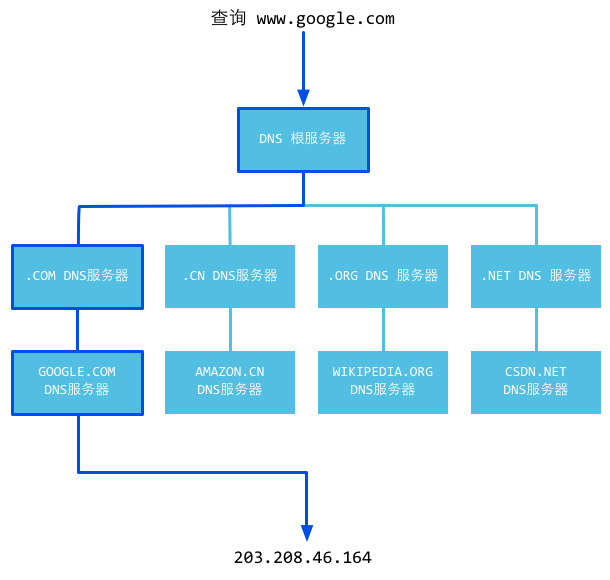
\includegraphics[width=14cm]{3.1.dns_hierachy.png}
   \label{図3.2}
   \caption{DNSの動作原理}
\end{figure}


より詳細なDNS解決のプロセスは下のようなものです。このプロセスは我々がDNSの作業モードを理解するのに助けとなります。

\begin{enumerate}
  \item ブラウザでwww.qq.comドメインを入力します。オペレーティングシステムはまず自分のローカルのhostsファイルにこのアドレスがないか検査します。もしあれば、このIPアドレスの設定が適用されます。ドメイン解決終了。
  \item もしhostsにこのドメインの設定がなければ、ローカルのDNSリゾルバのバッファを探します。もしあれば、これを返します。ドメイン解決終了。
  \item もしhostsとローカルのDNSリゾルバのバッファのどちらにも目的のドメインがなかった場合、まずTCP/IPのオプションで設定されているプライマリDNSサーバを探します。ここではこれをローカルDNSサーバと呼びましょう。このサーバが要求を受けた時、もし要求したドメイン名がローカルで設定されたリソースの中に含まれている場合、解決の結果をクライアントに返します。ドメイン解決終了。これは権威ある解決です。
  \item もし要求したドメイン名がローカルDNSサーバのゾーンでは解決できなかったものの、このサーバがこのURLをバッファリングしていた場合このIPアドレスが適用されます。ドメイン名解決終了。これは権威ある解決ではありません。
  \item もしローカルDNSサーバがそのゾーンファイルとバッファリングのどちらも有効でなかった場合、ローカルDNSサーバの設定に従って(リピータが設定されているか)検査を行います。もし転送モードが使用されていなければローカルDNSはリクエストを"ルートDNSサーバ"に送ります。"ルートDNSサーバ"はリクエストを受け取った後このドメイン名(.com)が誰によって権限を受け管理されているか判断し、このトップレベルドメインの権威サーバのIPを返します。ローカルDNSサーバがIP情報を受け取った後、.comドメインを担当するこのサーバと接続を行います。.comドメインを担当するサーバがリクエストを受け取った後、もし自分で名前解決できなければ、.comドメインを管理するもう一つ下のレイヤーのDNSサーバのアドレス(qq.com)をローカルDNSサーバに送ります。ローカルDNSサーバがこのアドレスを受け取った後、qq.comドメインのサーバを探し出し、www.qq.comのホストが見つかるまで上の動作を繰り返します。
  \item もし転送モードを使用していれば、このDNSサーバはリクエストをひとつ上のレイヤーのDNSサーバに転送します。このサーバが名前解決を行い、名前が解決できなかった場合は、ルートDNSを探すか、もう一つ上のレイヤーのにリクエストを転送します。またはルートが提示されます。最後に結果をローカルDNSサーバに返し、このDNSサーバはクライアントに返します。
\end{enumerate}


\begin{figure}[H]
  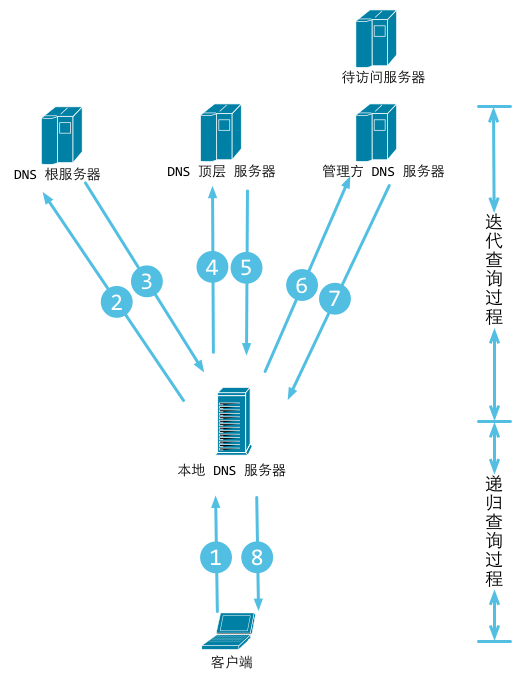
\includegraphics[width=14cm]{3.1.dns_inquery.png}
   \label{図3.3}
   \caption{DNS解決の全体のプロセス}
\end{figure}


\begin{quote}
いわゆる再帰検索プロセスは"検索者"の交代を意味します。また、反復する検索プロセスでは"検索者"は不変です。

例をあげて説明しましょう。あなたは一緒に法律の授業を受けている女の子の電話番号を知りたいとします。あなたはこっそり彼女の写真も撮っています。寝室にもどって、正義感の強いアニキたちにそのことを伝えます。このアニキたちは異議を唱えることもなく、胸を叩いてあなたにこう言います。「急ぐ必要はない。私があなたに替わって調べてあげましょう」(この時一時再帰検索が完了しています。すなわち、検索者の役割が変更されました。)。その後彼は写真を携え学部の4年生の先輩のところに聞きにいきます。「この女の子はxx学部なんですけど・・・」その後このアニキは矢継ぎ早にxx学部のオフィス主任の助手を務めているクラスメートに聞きます。このクラスメートはxx学部のyyゼミであると言います。またこの正義感の強いアニキたちはxx学部のyyゼミのゼミ長のところにいき、この女の子の電話番号をゲットします。(ここまでで何回かの連続検索が完了しました。すなわち、検索者の役は変わっていませんが、聞きに行く対象を反復して取り替えています。)最後に彼は番号をあなたの手に渡すことで全体の検索が完了します。
\end{quote}

上のステップを通して、IPアドレスを最後に取得します。つまりブラウザが最後にリクエストを送る時はIPにもとづいて、サーバと情報のやりとりをするのです。



\subsubsection{HTTPプロトコル詳細}
HTTPプロトコルはWeb作業の核心です。そのためWebの作業方法をくまなく理解するためには、HTTPがいったいどのような作業を行なっているのか深く理解する必要があります。

HTTPはWebサーバにブラウザ(クライアント)とInternetを通してデータをやり取りさせるプロトコルです。これはTCPプロトコルの上で成立しますので、一般的にはTCPの80番ポートが採用されます。これはリクエストとレスポンスのプロトコルです--クライアントはリクエストを送信しサーバがこのリクエストに対してレスポンスを行います。HTTPでは、クライアントは常に接続を行いHTTPリクエストを送信することでタスクをこなします。サーバは主導的にクライアントと接続することはできません。また、クライアントに対してコールバック接続を送信することもできません。クライアントとサーバは事前に接続を中断することができます。例えば、ブラウザでファイルをダウンロードする際、"停止"ボタンをクリックすることでファイルのダウンロードを中断し、サーバとのHTTP接続を閉じることができます。

HTTPプロトコルはステートレスです。同じクライアントの前のリクエストと今回のリクエストの間にはなんの対応関係もありません。HTTPサーバからすれば、この2つのリクエストが同じクライアントから発せられたものかすらも知りません。この問題を解決するため、WebプログラムではCookie機構を導入することで、接続の持続可能状態を維持しています。

\begin{quote}
HTTPプロトコルはTCPプロトコルの上で確立しますので、TCPアタックはHTTPの通信に同じように影響を与えます。例えばよく見かける攻撃として:SYN Floodは現在最も流行したDoS(サービス不能攻撃)とDdoS(分散型サービス不能攻撃)などがあります。これはTCPプロトコルの欠陥を利用して大量に偽造されたTCP接続要求を送信するのです。これにより攻撃された側はリソースが枯渇(CPUの高負荷やメモリ不足)する攻撃です。
\end{quote}

\subsubsection{HTTPリクエストパケット(ブラウザ情報)}
まずRequestパケットの構造を見てみることにしましょう。Requestパケットは3つの部分にわけられます。第一部分はRequest line(リクエスト行)。第二部分はRequest header(リクエストヘッダ)、第三部分はbody(ボディ)と呼ばれます。headerとbodyの間には空行があり、リクエストパケットの例は以下のようなものです。

\begin{lstlisting}[numbers=none]
GET /domains/example/ HTTP/1.1
//リクエスト行:リクエスト方法 リクエストRUI HTTPプロトコル/プロトコルバージョン
Host:www.iana.org  //サーバのホスト名
User-Agent:Mozilla/5.0 (Windows NT 6.1)
            AppleWebKit/537.4 (KHTML, like Gecko)
            Chrome/22.0.1229.94 Safari/537.4
//ブラウザ情報
Accept:text/html,application/xhtml+xml,
       application/xml;q=0.9,*/*;q=0.8    //クライアントが受け取れるmime
Accept-Encoding:gzip,deflate,sdch //ストリーム圧縮をサポートするか否か
Accept-Charset:UTF-8,*;q=0.5        //クライアントの文字コードセット
//空行、リクエストヘッダとボディを分けるために使われます。
//ボディ、リソースへのリクエストのオプション、例えばPOSTが渡すオプション
\end{lstlisting}

HTTPプロトコルはサーバに対して交互にリクエストを送る方法が定義されています。基本は四種類。GET,POST,PUT,DELETEです。ひとつのURLアドレスはひとつのネットワーク上のリソースを描写しています。またHTTPの中のGET, POST, PUT, DELETEはこのリソースの検索、修正、増加、削除の4つの操作に対応しています。よく見かけるのはGETとPOSTです。GETは一般的にリソースの情報を取得/検索するために用いられ、POSTはリソース情報を更新するために用いられます。

fiddlerパケットキャプチャを通して下のようなリクエスト情報を見ることができます。

\begin{figure}[H]
  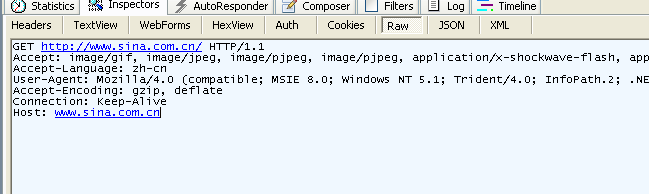
\includegraphics[width=14cm]{3.1.http.png}
   \label{図3.4}
   \caption{fiddlerがキャプチャしたGET情報}
\end{figure}


\begin{figure}[H]
  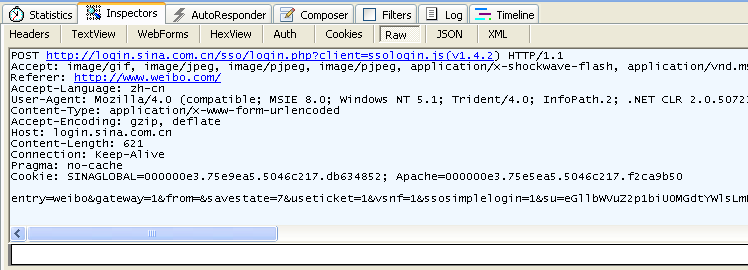
\includegraphics[width=14cm]{3.1.httpPOST.png}
   \label{図3.5}
   \caption{fiddlerがキャプチャしたPOST情報}
\end{figure}

GETとPOSTの区別を見てみましょう。

\begin{enumerate}
  \item GETリクエストのボディが空であることがわかります。POSTリクエストにはボディがあります。
  \item GETが入力するデータはURLの後に置かれます。?によってURLと渡すデータを分割します。オプションの間は\&で繋ぎます。例えばEditPosts.aspx?name=test1\&id=12345。POSTメソッドは入力するデータをHTTPパケットのBodyの中に置きます。
  \item GETが入力するデータの大きさには制限があります。(ブラウザのURLに対する長に制限があるためです。)またPOSTメソッドで入力するデータには制限がありません。
  \item GETメソッドで入力されたデータはセキュリティの問題を引き起こします。例えばログイン画面があったとして、GETメソッドでデータを入力した場合、ユーザ名とパスワードはURL上にあらわれてしまうことになります。もしページがバッファリングされていたり他の人によっがこのマシンにアクセスすることができれば、ヒストリログからこのユーザのアカウントとパスワードを取得することができてしまいます。
\end{enumerate}



\subsubsection{HTTPレスポンスパケット(サーバ情報)}
HTTPのresponseパケットを見てみることにしましょう。構造は以下のとおりです:

\begin{lstlisting}[numbers=none]
HTTP/1.1 200 OK     //ステータス行
Server: nginx/1.0.8 //サーバが使用するWEBソフトウェアの名称及びバージョン
Date:Date: Tue, 30 Oct 2012 04:14:25 GMT //送信時刻
Content-Type: text/html   //サーバが送信するデータの型
Transfer-Encoding: chunked //送信するHTTPパケットが分解されることを表しています。
Connection: keep-alive   //コネクション状態の保持
Content-Length: 90        //ボディの内容の長さ
//空行 ヘッダとボディを分けるために使われます。
<!DOCTYPE html PUBLIC "-//W3C//DTD XHTML 1.0 Transitional//EN"... //ボディ
\end{lstlisting}

レスポンスパケットの第一行はステータス行と呼ばれ、HTTPプロトコルバージョン番号、ステータスコード、及びステータスメッセージの3つの部分から構成されています。

ステータスコードはHTTPクライアントにHTTPサーバが事前にResponseを発生させるか伝えます。HTTP/1.1プロトコルでは5種類のステータスコードが定義されています。ステータスコードは3桁の数字で表されます。はじめの数字はレスポンスの型を定義しています。

\begin{description}
  \item[1XX] 情報の表示 - リクエストの取得に成功しました。継続して処理します。
  \item[2XX] 成功 - リクエストの取得に成功しました。わかりました。受け付けます。
  \item[3XX] リダイレクション - リクエストを完了させる為に一歩進んだ処理が必要です。
  \item[4XX] クライアントエラー - リクエストにシンタックスエラーまたはリクエストを実現できません。
  \item[5XX] サーバーエラー - サーバは合法なリクエストを実現できません。
\end{description}

下の図で詳細なレスポンス情報について説明しております。左側にたくさんのリソースのレスポンスコードを見ることができます。200は通常です。正常なデータであることを意味しています。302ははリダイレクトを意味します。response headerの中には詳細な情報が展開されています。

\begin{figure}[H]
  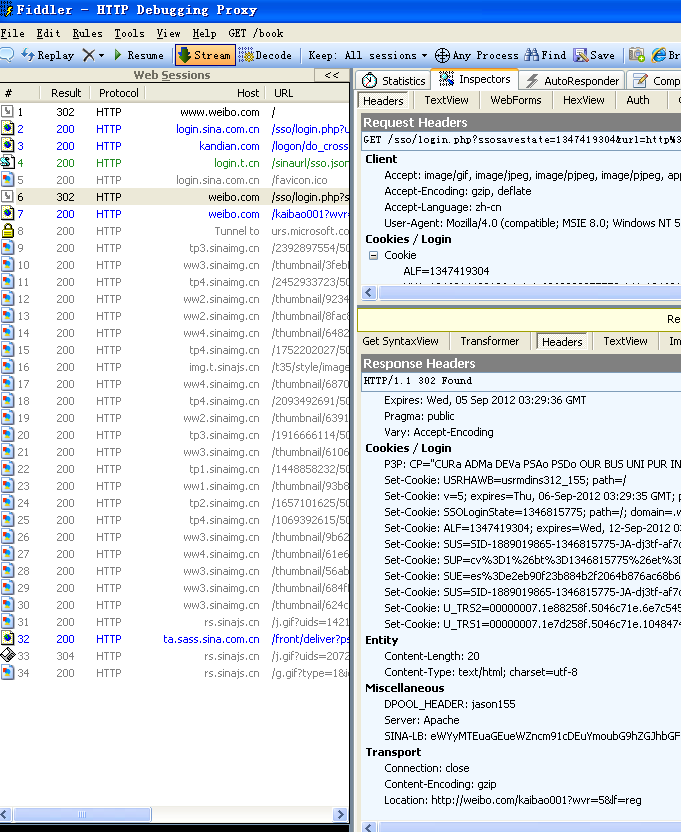
\includegraphics[width=14cm]{3.1.response.png}
   \label{図3.6}
   \caption{ホームページに一度訪問した場合のリクエスト情報のすべて}
\end{figure}



\subsubsection{HTTPプロトコルはステートレスでConnection: keep-aliveの区別}
ステートレスとはプロトコルがタスク処理に対して記憶力を有していないことを意味します。サーバはクライアントがどんな状態にあるか知らず、別の角度から言えば、サーバ上のホームページを開いたのと、あなたが以前このサーバ上のホームページを開いた事との間には何の関係もないことを意味しています。

HTTPはステートレスなコネクション指向のプロトコルです。ステートレスとはHTTPがTCP接続を保持していないことを意味するものではありません。また、HTTPがUDPプロトコルを使っていることを示すものでもありません。(コネクションロスに対して)

HTTP/1.1から、デフォルトでKeep-Aliveがオンになっており、接続性が保持されます。簡単にいえば、あるホームページを開き終わった後、クライアントとサーバの間ではHTTPデータを転送するためのTCP接続は閉じません。もしクライアントが再度このサーバ上のホームページを開いた場合、すでに確立されたTCP接続を継続して使用し得ます。

Keep-Aliveは永久にコネクションを保持するものではありません。これには保持する時間があります。異なるサーバソフトウェア(例えばApache)ではこの時間を設定することができます。

\subsubsection{リクエスト実例}
\begin{figure}[H]
  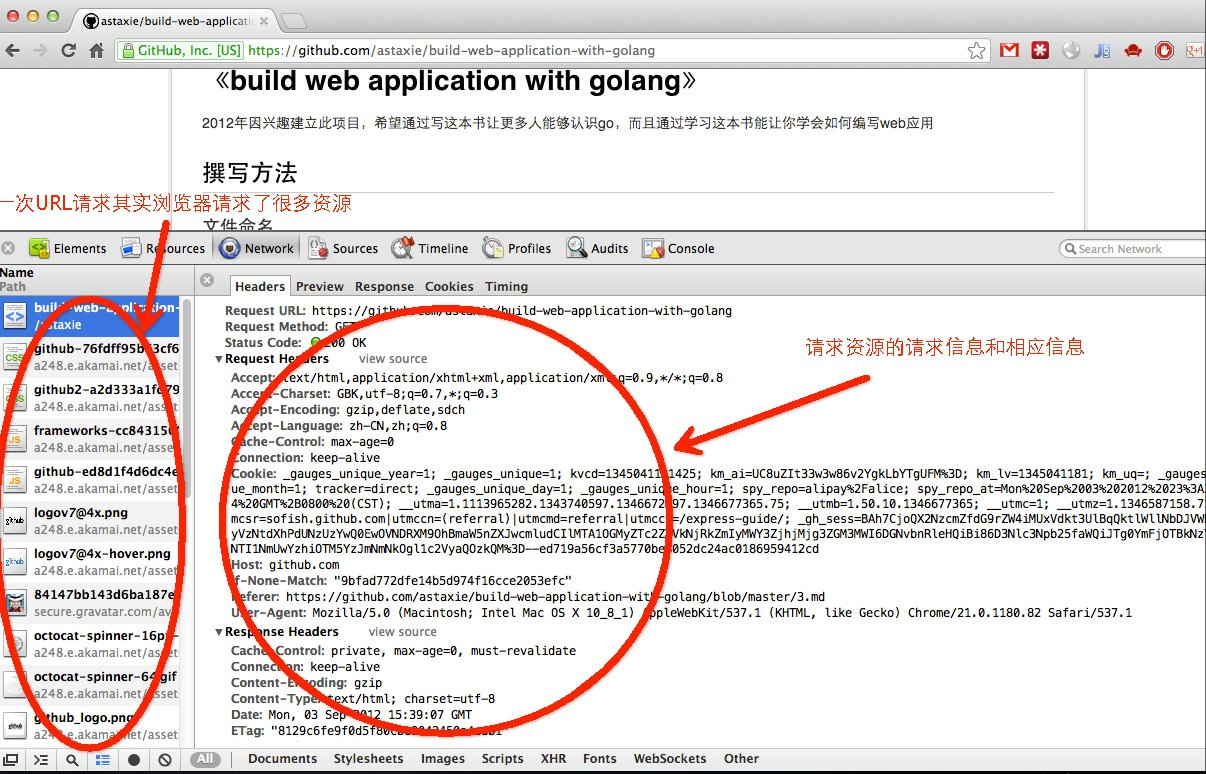
\includegraphics[width=14cm]{3.1.web.jpg}
   \label{図3.7}
   \caption{一回の要求のrequestとresponse}
\end{figure}



上の図で全体の通信プロセスをご理解いただけるかと思います。同時に注意深い読者はひとつのURLリクエストにもかかわらず左のペインではどうしてこのように多くのリソース要求があるのかと思われたかもしれません。(これらはすべて静的なファイルです。goは静的なファイルに対して専門的に処理する方法を有しています。)

これはブラウザの機能の一つです。URLを一度要求すると、サーバはhtmlページを返します。その後ブラウザはHTMLを読み取り、HTMLのDOMの中にあるイメージリンク、cssスクリプトとjsスクリプトのリンクを見つけた時、ブラウザは自動的に静的なリソースのHTTP要求を行います。目的の静的なリソースを取得すると、ブラウザは読み始めます。最後にすべてのリソースを整理し、我々の前のスクリーン上に展開します。

\begin{quote}
ホームページの改良では、HTTPのリクエスト回数を減らすことがあります。つまり、なるべく多くのcssとjsリソースを同じところに集めるのです。目的は出来る限りホームページの静的リソースのリクエスト回数を減少させる事にあります。ホームページの表示速度を上げると同時にサーバのバッファリングを減らす事ができます。
\end{quote}


\subsection{Goで簡単なwebサーバを立てる}
前の節でWebはhttpプロトコルに基づいたサービスであるとご紹介しました。Go言語では完全なnet/httpパッケージを提供しています。httpパッケージを通して実行できるWebサービスを非常に簡単に立ち上げる事ができます。同時にこのパッケージを使用することで、簡単にWebのルーティング、静的なファイル、テンプレート、cookie等のデータに対して設定と操作を行うことができます。


\subsubsection{httpパッケージでWebサーバを立てる}
\begin{lstlisting}[numbers=none]
package main

import (
    "fmt"
    "net/http"
    "strings"
    "log"
)

func sayhelloName(w http.ResponseWriter, r *http.Request) {
    r.ParseForm()  //オプションを解析します。
                   //デフォルトでは解析しません。
    fmt.Println(r.Form)
    //このデータはサーバのプリント情報に出力されます。
    fmt.Println("path", r.URL.Path)
    fmt.Println("scheme", r.URL.Scheme)
    fmt.Println(r.Form["url_long"])
    for k, v := range r.Form {
        fmt.Println("key:", k)
        fmt.Println("val:", strings.Join(v, ""))
    }
    fmt.Fprintf(w, "Hello astaxie!")
    //ここでwに入るものがクライアントに出力されます。
}

func main() {
    http.HandleFunc("/", sayhelloName)
    //アクセスのルーティングを設定します。
    err := http.ListenAndServe(":9090", nil)
    //監視するポートを設定します。
    if err != nil {
        log.Fatal("ListenAndServe: ", err)
    }
}
\end{lstlisting}

上のコードはbuildした後、web.exeを実行した際、9090ポートでhttpリンクリクエストを監視します。

ブラウザで\texttt{http:\/\//\/\//localhost:9090}を入力してください。

ブラウザでHello astaxie!と出力されたのが見えたかと思います。

アドレスを変えて試してみましょう:\texttt{http:\//\//localhost:9090\//?url\_long=111\&url\_long=222}

ブラウザで出力されたものは何でしょうか。サーバは何と出力していますか?

サーバで出力される情報は以下の通りです:

\begin{figure}[H]
  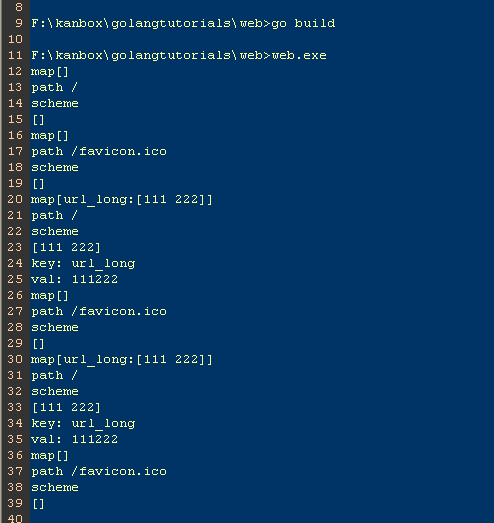
\includegraphics[width=14cm]{3.2.goweb.png}
   \label{図3.8}
   \caption{ユーザがWebにアクセスしてサーバが出力する情報}
\end{figure}

上のコードでWebサーバを書くためにはhttpパッケージの2つの関数を呼ぶだけで良いことがわかります。


\begin{quote}
もしあなたが以前PHPプログラマであれば。こう問うかもしれません。我々のnginx、apacheサーバは必要ないのですかと?なぜならこいつは直接tcpポートを監視しますので、nginxがやることをやってくれます。またsayhelloNameは実は我々が書いたロジック関数ですので、phpの中のコントローラ(controller)関数に近いものです。

もしあなたがPythonプログラマであったのなら、tornadoを聞いたことがあると思います。このコードはそれとよく似ていませんか?ええ、その通りです。GoはPythonのような動的な言語によく似た特性を持っています。Webアプリケーションを書くにはとても便利です。

もしあなたがRubyプログラマであったのなら、RORの/script/serverを起動したのと少し似ている事に気づいたかもしれません。
\end{quote}


Goを通じて簡単な数行のコードでwebサーバを立ち上げることができました。さらにこのWebサーバの内部ではマルチスレッドの特性をサポートしています。続く2つの節でGoが如何にWebのマルチスレッドを実現しているのか細かくご紹介します。



\subsection{Goはどのようにしてweb作業を行うか}
前の節でどのようにGoを通じてWebサービスを立てるかご紹介しました。net/httpパッケージを簡単に応用して便利に立てることができたかと思います。では、Goは低レイヤーで一体何を行なっているのでしょうか?万物は姿を変えてもその元は同じであります。GoのWebサービス作業も第一章でご紹介したWebの作業方法に関係しています。


\subsubsection{webの作業方法のいくつかの概念}
以下はどれもサーバの概念のいくつかです

\begin{description}
  \item[Request] ユーザが要求するデータ。ユーザのリクエスト情報を解析します。post、get、cookie、url等の情報を含みます。
  \item[Response] サーバがクライアントにデータをフィードバックする必要があります。
  \item[Conn] ユーザの毎回のリクエストリンクです。
  \item[Handler] リクエストを処理し、返すデータを生成する処理ロジック。
\end{description}

\subsubsection{httpパッケージが実行する機能を分析する}
下の図はGoが実現するWebサービスの作業モードのプロセス図です

\begin{figure}[H]
  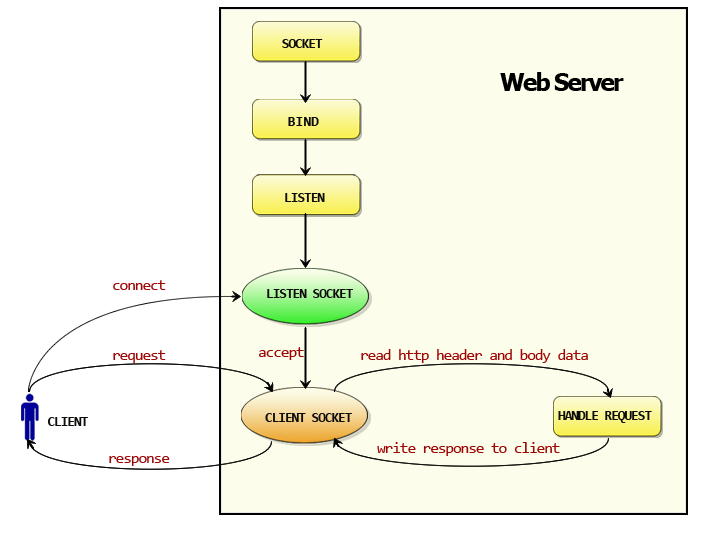
\includegraphics[width=14cm]{3.3.http.png}
   \label{図3.9}
   \caption{httpパッケージの実行フロー}
\end{figure}

\begin{enumerate}
  \item Listen Socketを作成し、指定したポートを監視します。クライアントのリクエストを待ちます。
  \item Listen Socketはクライアントのリクエストを受け付けます。Client Socketを得ると、Client Socketを通じてクライアントと通信を行います。
  \item クライアントのリクエストを処理します。まず、Client SocketからHTTPリクエストのプロトコルヘッダを読み取り、もしPOSTメソッドであれば、クライアントが入力するデータをさらに読み取るかもしれません。その後対応するhandlerがリクエストを処理します。handlerがクライアントの要求するデータを準備し終えたら、Client Socketを通じてクライアントに書き出します。
\end{enumerate}

この全体のプロセスでは3つの問題についてだけ理解しておけば構いません。これはまたGoがいかにしてWebを実行するのかということを知るという意味です。

\begin{itemize}
  \item どのようにポートを監視するか?
  \item クライアントのリクエストをどのように受け付けるか?
  \item handlerにどのように受け渡すか?
\end{itemize}

前の節のコードではGoは関数\texttt{ListenAndServe}を通してこれらの事を処理していました。ここでは実はこのように処理しています:serverオブジェクトを初期化します。その後\texttt{net.Listen("tcp", addr)}をコールします。つまり、低レイヤでTCPプロトコルを用いてサービスを立ち上げます。その後我々が設定したポートを監視します。

下のコードはGoのhttpパッケージのソースコードから引用したものです。下のコードで全体のHTTP処理プロセスを見ることができます。

\begin{lstlisting}[numbers=none]
func (srv *Server) Serve(l net.Listener) error {
    defer l.Close()
    var tempDelay time.Duration
                  // how long to sleep on accept failure
    for {
        rw, e := l.Accept()
        if e != nil {
            if ne, ok := e.(net.Error); ok && ne.Temporary() {
                if tempDelay == 0 {
                    tempDelay = 5 * time.Millisecond
                } else {
                    tempDelay *= 2
                }
                if max := 1 * time.Second; tempDelay > max {
                    tempDelay = max
                }
                log.Printf("http: Accept error: %v; retrying in %v",
                           e, tempDelay)
                time.Sleep(tempDelay)
                continue
            }
            return e
        }
        tempDelay = 0
        c, err := srv.newConn(rw)
        if err != nil {
            continue
        }
        go c.serve()
    }
}
\end{lstlisting}

監視した後どのようにしてクライアントのリクエストを受け取るのでしょうか?上のコードではポートの監視を実行後、\texttt{srv.Serve(net.Listener)}関数をコールしています。この関数はクライアントのリクエスト情報を処理しています。この関数では\texttt{for\{\}}が置かれており、まずListenerを通じてリクエストを受け取った後、Connを作成します。最後に単独のgoroutineを開きます。このリクエストのデータを引数としてこのconnに渡します。:\texttt{go c.serve()}。これはマルチスレッドを行なっています。ユーザが行うリクエストはすべて真新しいgoroutineの上で行われ、互いに影響しません。

ではいかにして具体的に目的の関数でリクエストを処理するように振り分けるのでしょうか?connはまずrequestを解析します:\texttt{c.readRequest()}、その後目的のhandlerを取得します:\texttt{handler := sh.srv.Handler}、つまり、我々がさきほど\texttt{ListenAndServe}をコールした時、その2つ目の引数です。前の例でnilを渡したのですが、これは空ということです。デフォルトで\texttt{handler = DefaultServeMux}を取得します。この変数は一体何に使われるのでしょうか?そうです。この変数はルータです。これはマッチするurlを対応するhandler関数にリダイレクトするために用いられます。我々はこれを設定したでしょうか?ええ。我々がコールしたコードのいの一番で\texttt{http.HandleFunc("/", sayhelloName)}をコールしたじゃないですか。これは\texttt{/}をリクエストするルートのルールを登録します。urlが"/"をリクエストした場合、ルートは関数sayhelloNameにリダイレクトします。DefaultServeMuxはServeHTTPメソッドをコールします。このメソッド内では実はsayhelloName本体をコールしています。最後にresponseの情報を入力することで、クライアントにフィードバックを返します。

全体のフローの詳細は以下の図の通りです:

\begin{figure}[H]
  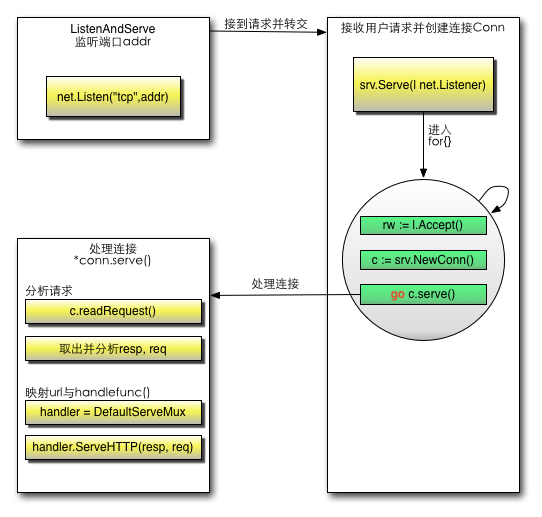
\includegraphics[width=14cm]{3.3.illustrator.png}
   \label{図3.10}
   \caption{http接続の処理フロー}
\end{figure}

ここに来て我々は3つの問題に対して全て解答を得ました。Goが如何にWebを走らせるか、すでに基本的なことは理解されたのではないでしょうか?


\subsection{Goのhttpパッケージ詳細}
前の節でGoが如何にWebの作業モードを実現するかフローをご紹介しました。この節では、httpパッケージを詳しく解剖していきます。これはどのように全体のプロセスを実現しているのでしょうか。

Goのhttpには2つのコアとなる機能があります:Conn、ServeMux

\subsubsection{Connのgoroutine}
我々が普段書くhttpサーバとは異なり、Goはマルチスレッドと高い性能を実現するため、goroutinesを使ってConnのイベント読み書きを処理します。これによって各リクエストは独立性を保持することができます。互いにブロックせず、効率よくネットワークイベントにレスポンスすることができます。これがGoに高い効率を保証します。

Goがクライアントのリクエストを待ち受けるには以下のように書きます:

\begin{lstlisting}[numbers=none]
c, err := srv.newConn(rw)
if err != nil {
    continue
}
go c.serve()
\end{lstlisting}

クライアントの各リクエストはどれもConnを一つ作成しているのがわかるかと思います。このConnには今回のリクエストの情報が保存されています。これは目的のhandlerに渡され、このhandlerで目的のhandler情報を読み取ることができます。このように各リクエストの独立性を保証します。


\subsubsection{ServeMuxのカスタム定義}
前の節でconn.serverについてご説明した際、拾は内部ではhttpパッケージのデフォルトのルートをコールしていました。ルータを通して今回のリクエストのデータをバックエンドの処理関数に渡します。ではこのルータはどのように実現されているのでしょうか?

構造は以下のとおりです:


\begin{lstlisting}[numbers=none]
type ServeMux struct {
    mu sync.RWMutex   //ミューテックス、リクエストが
                      //マルチスレッド処理に及んだことで
                      //ミューテックス機構が必要になります。
    m  map[string]muxEntry  // ルーティングルール、一つの
                            //stringがひとつのmuxエンティティ
                            //に対応します。ここではstringは
                            //登録されるルーティングを表現しています。
    hosts bool // 任意のルールにhost情報が含まれているか
}
\end{lstlisting}

以下でmuxEntryを見てみましょう

\begin{lstlisting}[numbers=none]
type muxEntry struct {
    explicit bool   // 精確にマッチするか否か
    h        Handler // このルーティング式はどのhandlerに対応するか
    pattern  string  //マッチング文字列
}
\end{lstlisting}

次にHandlerの定義を見てみましょう。

\begin{lstlisting}[numbers=none]
type Handler interface {
    ServeHTTP(ResponseWriter, *Request)  // ルーティング実現器
}
\end{lstlisting}

Handlerはインターフェースですが、前の節の中の\texttt{sayhelloName}関数では特にServeHTTPというインターフェースを実装してはいませんでした。どうして追加できるのでしょうか?もともとhttpパッケージの中では\texttt{HandlerFunc}という型が定義されています。私達が定義した\texttt{sayhelloName}関数はまさにこのHandlerFuncがコールされた結果であり、この型はデフォルトでServeHTTPインターフェースを実装していることになります。つまり、HandlerFunc(f)をコールして強制的にfをHandlerFunc型に型変換しているのです。このようにしてfはServeHTTPメソッドを持つようになります。

\begin{lstlisting}[numbers=none]
type HandlerFunc func(ResponseWriter, *Request)

// ServeHTTP calls f(w, r).
func (f HandlerFunc) ServeHTTP(w ResponseWriter, r *Request) {
    f(w, r)
}
\end{lstlisting}

ルータでは対応するルーティングルールを保存した後、具体的にはどのようにリクエストを振り分けているのでしょうか?以下のコードをご覧ください。デフォルトのルータは\texttt{ServeHTTP}を実装します:

\begin{lstlisting}[numbers=none]
func (mux *ServeMux) ServeHTTP(w ResponseWriter, r *Request) {
    if r.RequestURI == "*" {
        w.Header().Set("Connection", "close")
        w.WriteHeader(StatusBadRequest)
        return
    }
    h, _ := mux.Handler(r)
    h.ServeHTTP(w, r)
}
\end{lstlisting}

上に示す通りルータはリクエストを受け取った後、\texttt{*}であれば接続を切断し、そうでなければ\texttt{mux.handler(r).ServeHTTP(w, r)}をコールして対応する設定された処理Handlerを返し、\texttt{h.ServeHTTP(w, r)}を実行します。

つまり、目的のルーティングのhandlerのServerHTTPインターフェースへのコールです。ではmux.Handler(r)はどのように処理するのでしょうか?

\begin{lstlisting}[numbers=none]
func (mux *ServeMux) Handler(r *Request) (h Handler, pattern string) {
    if r.Method != "CONNECT" {
        if p := cleanPath(r.URL.Path); p != r.URL.Path {
            _, pattern = mux.handler(r.Host, p)
            return RedirectHandler(p, StatusMovedPermanently), pattern
        }
    }    
    return mux.handler(r.Host, r.URL.Path)
}

func (mux *ServeMux) handler(host, path string) (h Handler, pattern string) {
    mux.mu.RLock()
    defer mux.mu.RUnlock()

    // Host-specific pattern takes precedence over generic ones
    if mux.hosts {
        h, pattern = mux.match(host + path)
    }
    if h == nil {
        h, pattern = mux.match(path)
    }
    if h == nil {
        h, pattern = NotFoundHandler(), ""
    }
    return
}
\end{lstlisting}

もともとこれはユーザのリクエストしたURLとルータの中に保存されているmapに従ってマッチングしています。マッチングによって保存されているhandlerが返されるにあたり、このhandlerのServeHTTPインターフェースがコールされ、目的の関数を実行することができます。

上の紹介を通して、私達はルーティングの全体プロセスを理解しました。Goは実は外部で実装されたルータをサポートしています。\texttt{ListenAndServe}の第2引数が外部のルータを設定する為に用いられます。これはHandlerインターフェースのひとつで、外部ルータでHandlerインターフェースを実装し、そのServeHTTPにカスタム定義のルーティング機能を実装することができます。

下のコードを通して、自分自身で簡単なルータを実装してみます。

\begin{lstlisting}[numbers=none]
package main

import (
    "fmt"
    "net/http"
)

type MyMux struct {
}

func (p *MyMux) ServeHTTP(w http.ResponseWriter, r *http.Request) {
    if r.URL.Path == "/" {
        sayhelloName(w, r)
        return
    }
    http.NotFound(w, r)
    return
}

func sayhelloName(w http.ResponseWriter, r *http.Request) {
    fmt.Fprintf(w, "Hello myroute!")
}

func main() {
    mux := &MyMux{}
    http.ListenAndServe(":9090", mux)
}
\end{lstlisting}




\subsubsection{Goのコードの実行プロセス}
httpパッケージへの分析を通して、全体のコードの実行プロセスを整理してみましょう。

\begin{itemize}
  \item まずHttp.HandleFuncをコールします。\\ 順序にしたがっていくつかの事を行います:
  \begin{enumerate}
  \item DefaultServeMuxのHandlerFuncをコールする。
  \item DefaultServeMuxのHandleをコールする。
  \item DefaultServeMuxのmap[string]muxEntryで目的のhandlerとルーティングルールを追加する。
  \end{enumerate}
  \item 次にhttp.ListenAndServe(":9090", nil)をコールする。\\ 順序にしたがっていくつかの事を行う:
  \begin{enumerate}
  \item Serverのエンティティ化
  \item ServerのListenAndServe()をコールする
  \item net.Listen("tcp", addr)をコールし、ポートを監視する
  \item forループを起動し、ループの中でリクエストをAcceptする
  \item 各リクエストに対してConnを一つエンティティ化し、このリクエストに対しgoroutineを一つ開いてgo c.serve()のサービスを行う。
  \item 各リクエストの内容を読み込むw, err := c.readRequest()
  \item handlerが空でないか判断する。もしhandlerが設定されていなければ(この例ではhandlerは設定していません)、handlerはDefaultServeMuxに設定されます。
  \item handlerのServeHttpをコールする
  \item この例の中では、この後DefaultServeMux.ServeHttpの中に入ります
  \item requestに従ってhandlerを選択し、このhandlerのServeHTTPに入ります
    \begin{lstlisting}[numbers=none]
mux.handler(r).ServeHTTP(w, r)
  \end{lstlisting}
  \item handlerを選択します:
\begin{itemize}
  \item ルータがこのrequestを満足したか判断します(ループによってServerMuxのmuxEntryを走査します。)
  \item もしルーティングされれば、このルーティングhandlerのServeHttpをコールします。
  \item ルーティングされなければ、NotFoundHandlerのServeHttpをコールします
\end{itemize}
  \end{enumerate}
\end{itemize}


\subsection{まとめ}
この章ではHTTPプロトコル、DNS名前解決のプロセス、どのようにしてgoで簡単なweb serverを実装するかご紹介しました。net/httpパッケージのソースコードに触れるうちにこのserverを実装する秘密についてお分かりいただけたかと思います。

この章の学習を通じて、GoによるWeb開発の初歩をご理解いただければ幸いです。我々はまた対応するコードを見ることでGoでWebアプリケーションを開発することがとても便利でまた相当柔軟であると分かりました。



\section{フォーム}
フォームは普段Webアプリケーションを書く時によく使われるツールです。フォームを通して便利にユーザにサーバとデータをやり取りさせることができます。以前にWeb開発をしたことのあるユーザにとってはフォームはとてもお馴染みのものです。しかしC/C++のプログラマからすると少々取っ付きにくいかもしれません。フォームとは一体何でしょうか?

フォームは表の要素を含むエリアです。フォームの要素はユーザがフォームの中で(例えば、テキストフィールド、コンボボックス、チェックボックス、セレクトボックス等です。)情報を入力する要素です。フォームはフォームタグ(\textbackslash)で定義します。

\begin{lstlisting}[numbers=none]
<form>
...
input 要素
...
</form>
\end{lstlisting}

Goではformの処理に簡単な方法が既に用意されています。Requestの中にformを専門に処理するものがあり、簡単にWeb開発に利用できます。4.1節の中でGoがどのようにフォームの入力を処理するかご説明します。いかなるユーザの入力も信用はできないので、これらの入力に対し検証を行う必要があります。4.2節では一般的にどのように検証を行うか、細かいデモンストレーションを行います。

HTTPプロトコルはステートレスなプロトコルです。ではどのようにして一人のユーザを同定するのでしょうか?また、フォームが複数回送信されてしまわないように保証するにはどうするのでしょうか?4.3と4.4節ではcookie(cookieはクライアントに保存される情報です。HTTP Headerを通してサーバーとやり取りされます)等をより詳しくご紹介します。

フォームにはもうひとつファイルをアップロードできるという大きな機能があります。Goはファイルのアップロードをどのように処理しているのでしょうか?大きなファイルをアップロードする際効率よく処理するにはどうすればよいでしょうか?4.5節ではGoによるファイルのアップロード処理の知識を一緒に勉強します。



\subsection{フォームの入力を処理する}
まずフォームによる送信の例を見てみましょう。以下のようなフォームのコンテンツがあるとします。login.gtplというファイルを新規作成します。(新しくディレクトリを作ってその中に入れてください)

\begin{lstlisting}[numbers=none]
<html>
<head>
<title></title>
</head>
<body>
<form action="/login" method="post">
    ユーザ名:<input type="text" name="username">
    パスワード:<input type="password" name="password">
    <input type="submit" value="ログイン">
</form>
</body>
</html>
\end{lstlisting}

上で送信されるフォームはサーバの\texttt{/login}に渡されます。ユーザが情報を入力しログインをクリックした後、サーバのルーティングの\texttt{login}にリダイレクトします。まずはこの送信が何のメソッドによるものか判断する必要があります。POSTでしょうかGETでしょうか?

httpパッケージにはそれを取得するとても簡単な方法があります。前のwebの例を基礎にloginページのformデータをどのように処理するか見てみましょう。



\begin{lstlisting}[numbers=none]
package main

import (
    "fmt"
    "html/template"
    "log"
    "net/http"
    "strings"
)

func sayhelloName(w http.ResponseWriter, r *http.Request) {
    r.ParseForm()       //urlが渡すオプションを解析します。
                        //POSTに対してはレスポンスパケットの
                        //ボディを解析します(request body)
    //注意:もしParseFormメソッドがコールされなければ、
    // 以下でフォームのデータを取得することができません。
    //これらのデータはサーバのプリント情報に出力されます
    fmt.Println(r.Form)
    fmt.Println("path", r.URL.Path)
    fmt.Println("scheme", r.URL.Scheme)
    fmt.Println(r.Form["url_long"])
    for k, v := range r.Form {
        fmt.Println("key:", k)
        fmt.Println("val:", strings.Join(v, ""))
    }
    fmt.Fprintf(w, "Hello astaxie!")
    //ここでwに書き込まれたものがクライアントに出力されます。
}

func login(w http.ResponseWriter, r *http.Request) {
    fmt.Println("method:", r.Method) //リクエストを取得するメソッド
    if r.Method == "GET" {
        t, _ := template.ParseFiles("login.gtpl")
        t.Execute(w, nil)
    } else {
        //ログインデータがリクエストされ、
        //ログインのロジック判断が実行されます。
        fmt.Println("username:", r.Form["username"])
        fmt.Println("password:", r.Form["password"])
    }
}

func main() {
    //アクセスのルーティングを設定します
    http.HandleFunc("/", sayhelloName)
    //アクセスのルーティングを設定します
    http.HandleFunc("/login", login)
    //監視するポートを設定します
    err := http.ListenAndServe(":9090", nil)
    if err != nil {
        log.Fatal("ListenAndServe: ", err)
    }
}
\end{lstlisting}

上のコードにおいてリクエストのメソッドを取得するには\texttt{r.Method}だけで済むことがわかります。これは文字列型の変数です。GET, POST, PUT等のmethod情報を返します。

login関数では\texttt{r.Method}に従ってログイン画面を表示するのかログインロジックを処理するのかが判断されます。GETメソッドによるリクエストの場合はログイン画面を表示し、その他のメソッドによるリクエストではログインロジックを処理します。例えばデータベースを検索したり、ログイン情報を検証したりといった事です。

ブラウザで\texttt{http://127.0.0.1:9090/login}を開いた時に以下のような画面が現れます。

\begin{figure}[H]
  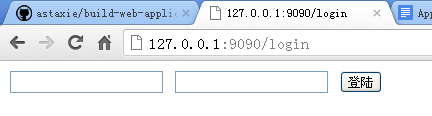
\includegraphics[width=14cm]{4.1.login.png}
   \label{図4.1}
   \caption{ユーザログイン画面}
\end{figure}

我々がユーザ名とパスワードを入力してもサーバは何も出力しません。なぜでしょうか?デフォルトではHandlerの中ではformの内容を自動的に解析しないからです。必ず明示的に\texttt{r.ParseForm()}をコールした後でなければ、このフォームのデータに対して操作を行うことはできません。コードを少し修正して、\texttt{fmt.Println("username:", r.Form["username"])}の前に\texttt{r.ParseForm()}という一行を追加してください。再コンパイルしてもう一度入力、送信してみると、今度はサーバがあなたの入力したユーザ名とパスワードを出力するはずです。

\texttt{r.Form}では全てのリクエストのデータが含まれています。例えばURLの中のquery-string、POSTのデータ、PUTのデータなどです。URLのquery-stringフィールドとPOSTが衝突する場合はsliceに保存されます。これには複数の値が保存されています。Goのオフィシャルドキュメントでは次のバージョンでPOST、GETといったデータは分離されると述べています。

ではlogin.gtplのformのaction値である\texttt{http://127.0.0.1:9090/login}を\texttt{http://127.0.0.1:9090/login?username=astaxie}に変更してもういちど試してみましょう。サーバが出力するusernameはsliceになっていませんか。サーバの出力は以下のようになります:

\begin{figure}[H]
  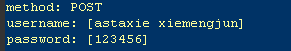
\includegraphics[width=7cm]{4.1.slice.png}
   \label{図4.1}
   \caption{サーバが受け取ったデータを表示}
\end{figure}

\texttt{request.Form}はurl.Values型です。この中には\texttt{key=value}のような対応するデータが保存されています。ここではformデータに対していくつかの操作をご紹介します:

\begin{lstlisting}[numbers=none]
v := url.Values{}
v.Set("name", "Ava")
v.Add("friend", "Jess")
v.Add("friend", "Sarah")
v.Add("friend", "Zoe")
// v.Encode() == "name=Ava&friend=Jess&friend=Sarah&friend=Zoe"
fmt.Println(v.Get("name"))
fmt.Println(v.Get("friend"))
fmt.Println(v["friend"])
\end{lstlisting}

\begin{quote}
\textbf{Tips}: RequestそのものもFormValue()関数でユーザが送信したデータを取得できます。例えばr.Form["username"]はr.FormValue("username")とも書けます。r.FormValueをコールした時は自動的にr.ParseFormがコールされますので、事前にコールする必要はありません。r.FormValueは同名のデータの中から一つ目のものだけを返します。もしデータが存在しない場合は空文字列を返します。
\end{quote}




\subsection{フォームに入力された内容の検証}
Web開発にはユーザが入力したいかなる情報も信用してはならないという原則があります。そのためユーザの入力した情報を検証しフィルターすることは非常に重要になってきます。ブログやニュースの中でどこそこのホームページがハッキングされたりセキュリティホールが存在するといったことをよく聞くかもしれません。これらの大部分はユーザの入力した情報に対してホームページが厳格な検証を行わなかった事によるものです。そのため、安全なWebプログラムを書くために、フォームの入力を検証する意義は非常に大きいのです。

Webアプリケーションを書く時は主に2つの場所でデータ検証を行います。ひとつはページ上でのJavaScriptによる検証で(現在この方面では多くのプラグインがあります。例えばValidationJSプラグインなどがそうです)、もうひとつはサーバ側での検証です。この節ではどのようにサーバでの検証を行うか解説します。

\subsubsection{必須フィールド}
あるフォーム要素から一つの値を取り出したいとします。例えば前の節のユーザ名はどのように処理するのでしょうか?Goにはbuiltin関数\texttt{len}があり、文字列の長さを得ることができます。lenを使ってデータの長さを測ることができます。例えば:


\begin{lstlisting}[numbers=none]
if len(r.Form["username"][0])==0{
    //空だった場合の処理
}
\end{lstlisting}

\texttt{r.Form}は異なる型のフォーム要素の空白に対して異なる処理を行います。空のテキストフィールド、テキストエリアおよびファイルアップロードに対して、その要素の値を空にします。また選択されていないコンボボックスやセレクトボックスr.Formの中にはそもそもその項目を作りません。上の例の中の方法でデータを取得した時プログラムはエラーを発生させます。そのため、\texttt{r.Form.Get()}を使って値を取る必要があります。なぜなら、もしフィールドが存在しなかった場合、この方法で取得すると空の値を得るからです。ですが、\texttt{r.Form.Get()}は単体の値しか得ることができません。もしmapの値であれば必ず上の方法で得る必要があります。

\subsubsection{数}
例えばフォームからある人の年齢が50歳や10歳といった具体的な値を必要としていて、"おっさん"とか"まだ若い"というようなものでなかったとします。このようにフォームの入力フィールドの中で数字のみを許容するようにさせたい場合、整数かどうかを判断するために、まずint型に変換を行ってから処理を行います。

正の整数を判断しようとする場合は、まずint型に変換してから処理を行います

\begin{lstlisting}[numbers=none]
getint,err:=strconv.Atoi(r.Form.Get("age"))
if err!=nil{
    //数の変換でエラーが発生。つまり、数字ではありません。
}

//次にこの数の取りうる範囲を判断します。
if getint >100 {
    //大きすぎる
}
\end{lstlisting}

もう一つの方法は正規表現による方法です。

\begin{lstlisting}[numbers=none]
if m, _ := regexp.MatchString("^[0-9]+$", r.Form.Get("age")); !m {
    return false
}
\end{lstlisting}

性能の高さを必要とするユーザからすればこれはよく話題にのぼる問題です。彼らはなるべく正規表現を避けるべきだと考えています。なぜなら正規表現の速度は一般的に遅いからです。しかし現在のようにコンピュータの性能がこれほど発達した時代では、このように簡単な正規表現の効率と型変換関数の間ではそれほど大きな差はありません。もしあなたが正規表現に詳しく、他の言語でも使用されているのであれば、Goの中で正規表現を使うのは便利な方法の一つです。

\begin{quote}
Goの正規表現の実装はRE2(http://code.google.com/p/re2/wiki/Syntax)です。すべての文字はUTF-8エンコーディングです。
\end{quote}



\subsubsection{中国語}
フォームの要素からユーザの中国語名を得たい場合で、なおかつ正しい中国語であることを保証したい場合、検証を行う必要があります。ユーザに自由に入力はさせません。中国語に対する有効な検証には、\texttt{unicode} パッケージが提供する \texttt{func Is(rangeTab *RangeTable, r rune) bool} と正規表現を使う方法があります。下のコードをご確認ください

\begin{lstlisting}[numbers=none]
if m, _ := regexp.MatchString("^\\p{Han}+$", r.Form.Get("realname")); !m {
    return false
}
\end{lstlisting}

\subsubsection{英語}
あるユーザの英語名を知りたいときなど、フォームの要素から英語の値を取り出したい場合は、astaxieであってasta謝ではないはずです。(訳注:「謝」はピンインでxieと書く)


簡単な正規表現を使ってデータを検証することができます:

\begin{lstlisting}[numbers=none]
if m, _ := regexp.MatchString("^[a-zA-Z]+$", r.Form.Get("engname")); !m {
    return false
}
\end{lstlisting}

\subsubsection{メールアドレス}
ユーザが入力したEmailアドレスが正しいか確認したい場合は以下のような方法で検証できます:

\begin{lstlisting}[numbers=none]
if m, _ := regexp.MatchString(`^([\w\.\_]{2,10})@(\w{1,}).([a-z]{2,4})$`,
                              r.Form.Get("email")); !m {
    fmt.Println("no")
}else{
    fmt.Println("yes")
}
\end{lstlisting}

\subsubsection{携帯電話番号}
ユーザが入力した携帯電話番号が正しいか判断したい場合は以下の正規表現で検証できます(訳注:中国の携帯電話番号):

\begin{lstlisting}[numbers=none]
if m, _ := regexp.MatchString(`^(1[3|4|5|8][0-9]\d{4,8})$`,
                              r.Form.Get("mobile")); !m {
    return false
}
\end{lstlisting}

\subsubsection{プルダウンメニュー}
フォームの中の\texttt{<select>}要素が生成するプルダウンメニューにおいて、ハッカーは時々このプルダウンメニューに無い項目を偽造してあなたに送りつけるかもしれません。このような場合値がもともと設定されたものであることを判断するにはどうすればよいでしょうか?

selectには以下の要素があるとします:


\begin{lstlisting}[numbers=none]
<select name="fruit">
<option value="apple">apple</option>
<option value="pear">pear</option>
<option value="banane">banane</option>
</select>
\end{lstlisting}

この場合は以下のように検証することができます

\begin{lstlisting}[numbers=none]
slice:=[]string{"apple","pear","banane"}

for _, v := range slice {
    if v == r.Form.Get("fruit") {
        return true
    }
}
return false
\end{lstlisting}


\subsubsection{ラジオボタン}
男と女という性別の選択肢を出力するようなラジオボタンでどれかが選択されているか判断するとします。15歳の退屈な少年がhttpプロトコルの本を片手にtelnetクライアントからあなたのプログラムに対してリクエストを送信したとしましょう。あなたは男に1を、女に2を設定していて、彼が3という値を送信した場合、あなたのプログラムは例外を出すでしょうか?プルダウンメニューの判断と同じように我々が得ようとしている値がそもそも設定されたものであるかを判断しなければなりません。

\begin{lstlisting}[numbers=none]
<input type="radio" name="gender" value="1">男
<input type="radio" name="gender" value="2">女
\end{lstlisting}

プルダウンメニューの方法と同じように行うことができます

\begin{lstlisting}[numbers=none]
slice:=[]int{1,2}

for _, v := range slice {
    if v == r.Form.Get("gender") {
        return true
    }
}
return false
\end{lstlisting}

\subsubsection{チェックボックス}
趣味を選択するチェックボックスがあり、ユーザが選択したものとあなたがユーザに提供した選択が同じ型のデータであることを保証する場合

\begin{lstlisting}[numbers=none]
<input type="checkbox" name="interest" value="football">サッカー
<input type="checkbox" name="interest" value="basketball">バスケットボール
<input type="checkbox" name="interest" value="tennis">テニス
\end{lstlisting}

チェックボックスではラジオボタンの時とくらべ検証方法が少し異なります。受け取るデータはsliceだからです。

\begin{lstlisting}[numbers=none]
slice:=[]string{"football","basketball","tennis"}
a:=Slice_diff(r.Form["interest"],slice)
if a == nil{
    return true
}

return false
\end{lstlisting}

上の\texttt{Slice\_diff}という関数には私のオープンソースのライブラリが含まれます(sliceとmapを操作するライブラリ)https://github.com/astaxie/beeku


\subsubsection{日付と時間}
ユーザが入力した日時が有効か確認したいとします。例えばユーザがスケジュールで8月45日にパーティを開く予定を入力したり、未来の時間を誕生日にしてみたりといった場合です。

Goではtimeの処理パッケージを提供しています。ユーザの入力した年月日を目的の時間に変換してから、判断を行います。

\begin{lstlisting}[numbers=none]
t := time.Date(2009, time.November, 10, 23, 0, 0, 0, time.UTC)
fmt.Printf("Go launched at %s\n", t.Local())
\end{lstlisting}


timeを取得した後、多くの時間関数の操作を行うことができます。具体的な判断は自身の要件に合わせて調整してください。


\subsubsection{身分証明書番号}
フォームに入力された身分証明書を検証する場合、正規表現を使って簡単に検証できます。しかし身分証明書番号は15桁と18桁があるので2つとも検証しなければなりません。(訳注:中国では身分証明書に個人を特定する身分証明番号(以前は15桁、現在は18桁)が記載されています。)

\begin{lstlisting}[numbers=none]
//15桁の身分証明書の検証。15桁はすべて数字です。
if m, _ := regexp.MatchString(`^(\d{15})$`,
                              r.Form.Get("usercard")); !m {
    return false
}

//18桁の身分証明書の検証。18桁の前17桁は数字で、
//最後の一桁はチェックデジットです。
//数字または文字Xを取り得ます。
if m, _ := regexp.MatchString(`^(\d{17})([0-9]|X)$`,
                              r.Form.Get("usercard")); !m {
    return false
}
\end{lstlisting}

以上、よく使用されるサーバ側でのフォーム要素の検証をいくつかご紹介しました。このイントロダクションを通してGoによるデータ検証、特に正規表現での処理に対する理解が深まるよう願っています。



\subsection{クロスサイトスクリプティングの予防}
現在のホームページは大量の動的なコンテンツを含みユーザのエクスペリエンスを高めています。以前に比べてとても複雑になっています。いわゆる動的なコンテンツとはユーザの環境と要求に応じてWebアプリケーションが目的の内容を出力できることを指します。動的なホームページは"クロスサイトスクリプティング"(Cross Site Scripting、セキュリティ専門家が一般的にXSSと省略するもの)と呼ばれる攻撃を受けることがあります。

攻撃者は通常セキュリティホールのあるプログラム中にJavaScript、VBScript、ActiveXまたはFlashを挿入することでユーザを騙します。一旦攻撃が成功するとユーザアカウント情報が盗まれ、ユーザの設定を改ざんされてしまったり、cookieを盗みまたは汚染して悪意ある広告を埋め込んだりされます。

XSSに対する最も効果的な予防は以下の二種類を組み合わせることです:すべての入力データを検証し攻撃の検査をすること(これに関しては前の節でいくつかご紹介しました)。もうひとつは出力されるデータに対し適切な処理を行うことによってすでに挿入されてしまったいかなるスクリプトに対してもブラウザで実行されないようにすることです。

Goではどのようにこの効果的な防御を行なっているのでしょうか?Goのhtml/templateの中では以下のいくつかの関数によってエスケープすることができます。


\begin{itemize}
  \item func HTMLEscape(w io.Writer, b []byte) //bに対してエスケープを行い、wに出力する。
  \item func HTMLEscapeString(s string) string //sに対してエスケープを行い、結果の文字列を返す。
  \item func HTMLEscaper(args ...interface{}) string //複数の引数を同時にエスケープします。結果となる文字列を返します。
\end{itemize}

4.1節の例を見てみましょう。

\begin{lstlisting}[numbers=none]
fmt.Println("username:", template.HTMLEscapeString(r.Form.Get("username")))
//サーバ側に出力されます。
fmt.Println("password:", template.HTMLEscapeString(r.Form.Get("password")))
template.HTMLEscape(w, []byte(r.Form.Get("username")))
//クライアントに出力されます。
\end{lstlisting}

もし入力されたusernameが\texttt{<script>alert()</script>}だった場合、ブラウザ上では以下のように表示されます:

\begin{figure}[H]
  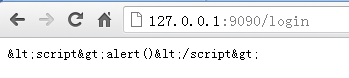
\includegraphics[width=8cm]{4.3.escape.png}
   \label{図4.3}
   \caption{Javascriptフィルターによる出力}
\end{figure}

Goのhtml/templateパッケージはデフォルトでhtmlタグをフィルターします。しかし時にはこの\texttt{<script>alert()</script>}を正常な情報として出力したい場合があるかもしれません。そのような場合はどのように処理するべきでしょうか?この場合はtext/templateをご利用ください。下の例をご覧ください: \texttt{import "text/template" ... t, err := template.New("foo").Parse(\{\{define "T"\}\}Hello, \{\{.\}\}!\{\{end\}\}) err = t.ExecuteTemplate(out, "T", "")}

出力

\begin{lstlisting}[numbers=none]
Hello, <script>alert('you have been pwned')</script>!
\end{lstlisting}

またはtemplate.HTML型を使用すると

\begin{lstlisting}[numbers=none]
import "html/template"
...
t, err := template.New("foo").Parse(`{{define "T"}}Hello,
                                    {{.}}!{{end}}`)
err = t.ExecuteTemplate(out, "T",
 template.HTML("<script>alert('you have been pwned')</script>"))
\end{lstlisting}

出力

\begin{lstlisting}[numbers=none]
Hello, <script>alert('you have been pwned')</script>!
\end{lstlisting}

\texttt{template.HTML}に変換した後も変数の内容はエスケープされません。

エスケープの例:

\begin{lstlisting}[numbers=none]
import "html/template"
...
t, err := template.New("foo").Parse(`{{define "T"}}Hello,
                                    {{.}}!{{end}}`)
err = t.ExecuteTemplate(out, "T",
           "<script>alert('you have been pwned')</script>")
\end{lstlisting}

エスケープ後の出力:

\begin{lstlisting}[numbers=none]
Hello, &lt;script&gt;alert(&#39;you have been pwned&#39;)&lt;/script&gt;!
\end{lstlisting}





\subsection{フォームの複数回送信の防止}
これまでにどこかのBBSやブログでご覧になったことがあるかもしれませんが、一つのスレッドや文章の後でいくつもの重複が記録されていることがあります。これらの大多数はユーザが複数回書き込みフォームを送信してしまったことによるものです。様々な原因でユーザはよくフォームを複数回送信してしまいます。通常はマウスの誤操作によるもので、送信ボタンをダブルクリックしてしまったり、一旦送信した内容を再度修正しようとして、ブラウザの戻るボタンを押した後に次へボタンではなくまた送信ボタンを押してしまうことによるものです。当然、故意によるものもあります。- - 例えばネット上のアンケート調査やくじ引きにおいて重複して投票するなどです。では、どのようにしてユーザが同じ内容のフォームの送信を行うことを効果的に防げるのでしょうか?

解決方法はフォームの中にユニークな値を持ったhiddenフィールドを追加することです。フォームを検証する際、このユニークな値を持ったフォームがすでに送信されているかどうか検証します。もしすでに送信されていれば、二回目の送信を拒絶します。そうでなければフォームに対して処理ロジックを行います。また、もしAjax形式で送信するフォームだった場合、フォームが送信された後javascriptによってフォームの送信ボタンを禁止します。

4.2節の例を改良してみましょう:

\begin{lstlisting}[numbers=none]
<input type="checkbox" name="interest" value="football">サッカー
<input type="checkbox" name="interest" value="basketball">バスケットボール
<input type="checkbox" name="interest" value="tennis">テニス
ユーザ名:<input type="text" name="username">
パスワード:<input type="password" name="password">
<input type="hidden" name="token" value="{{.}}">
<input type="submit" value="ログイン">
\end{lstlisting}

テンプレートの中に\texttt{token}というhiddenフィールドを追加しました。この値にはMD5(タイムスタンプ)によってユニークな値を割り当てます。この値をサーバに保存することで(sessionによるコントロールは6章でどのように保存するか解説します)フォームが送信される際の判定に使うことができます。

\begin{lstlisting}[numbers=none]
func login(w http.ResponseWriter, r *http.Request) {
    fmt.Println("method:", r.Method) //リクエストを受け取る方法
    if r.Method == "GET" {
        crutime := time.Now().Unix()
        h := md5.New()
        io.WriteString(h, strconv.FormatInt(crutime, 10))
        token := fmt.Sprintf("%x", h.Sum(nil))

        t, _ := template.ParseFiles("login.gtpl")
        t.Execute(w, token)
    } else {
        //リクエストはログインデータです。
        //ログインのロジックを実行して判断します。
        r.ParseForm()
        token := r.Form.Get("token")
        if token != "" {
            //tokenの合法性を検証します。
        } else {
            //tokenが存在しなければエラーを出します。
        }
        fmt.Println("username length:",
                    len(r.Form["username"][0]))
        fmt.Println("username:",
                    template.HTMLEscapeString(r.Form.Get("username")))
        //サーバ側に出力します。
        fmt.Println("password:",
                    template.HTMLEscapeString(r.Form.Get("password")))
        template.HTMLEscape(w, []byte(r.Form.Get("username")))
        //クライアントに出力します。
    }
}
\end{lstlisting}

出力されるページのソースは以下の通り:

\begin{figure}[H]
  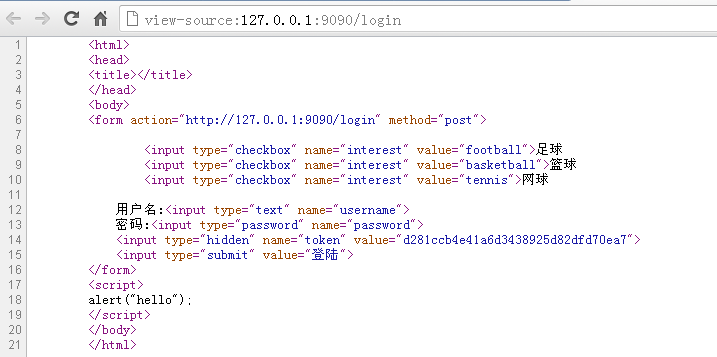
\includegraphics[width=14cm]{4.4.token.png}
   \label{図4.4}
   \caption{tokenを追加した後クライアントが出力するソース情報}
\end{figure}

tokenはすでに出力値を持っていますので連続してページを更新することができます。この値が次々と変化するのがお分かりいただけるかと思います。このように毎回formが表示される時にユニークになるよう保証します。ユーザが送信するフォームは唯一性が保持されます。

この解決方法は悪意の無い攻撃に対しても防止することができます。また悪意のあるユーザに対してもしばらく効果があります。その後、ユーザーにこの悪意のある動機を捨てさせることができなかった場合は更に複雑な作業が必要となります。


\subsection{ファイルのアップロード処理}
ユーザによるファイルのアップロードを処理したいとします。例えば、現在Instagramのようなホームページを作成しているとします。ユーザが撮影した写真を保存する必要があります。このような要求はどのように実現するのでしょうか?

フォームにファイルをアップロードさせるためには、まずformの\texttt{enctype}属性を追加する必要があります。\texttt{enctype}属性には以下の3つの種類があります:


\begin{lstlisting}[numbers=none]
application/x-www-form-urlencoded
     送信前にすべての文字列をエンコードする(デフォルト)
multipart/form-data
     文字列に対してエンコードしません。
     ファイルのアップロードウィジェットを含む
     フォームを使用するときはこの値が必要です。
text/plain
     空白を"+"記号に置き換えます。
     ただし、特殊文字に対してエンコードは行われません。
\end{lstlisting}

そのため、フォームのhtmlコードはこのようになります:

\begin{lstlisting}[numbers=none]
<html>
<head>
    <title>ファイルアップロード</title>
</head>
<body>
<form enctype="multipart/form-data"
      action="http://127.0.0.1:9090/upload"
      method="post">
  <input type="file" name="uploadfile" />
  <input type="hidden" name="token" value="{{.}}"/>
  <input type="submit" value="upload" />
</form>
</body>
</html>
\end{lstlisting}

サーバでは、handlerFuncをひとつ追加します:

\begin{lstlisting}[numbers=none]
http.HandleFunc("/upload", upload)

// /uploadを処理するロジック
func upload(w http.ResponseWriter, r *http.Request) {
    fmt.Println("method:", r.Method) //リクエストを受け取るメソッド
    if r.Method == "GET" {
        crutime := time.Now().Unix()
        h := md5.New()
        io.WriteString(h, strconv.FormatInt(crutime, 10))
        token := fmt.Sprintf("%x", h.Sum(nil))

        t, _ := template.ParseFiles("upload.gtpl")
        t.Execute(w, token)
    } else {
        r.ParseMultipartForm(32 << 20)
        file, handler, err := r.FormFile("uploadfile")
        if err != nil {
            fmt.Println(err)
            return
        }
        defer file.Close()
        fmt.Fprintf(w, "%v", handler.Header)
        f, err := os.OpenFile("./test/"+handler.Filename,
                              os.O_WRONLY|os.O_CREATE, 0666)
        if err != nil {
            fmt.Println(err)
            return
        }
        defer f.Close()
        io.Copy(f, file)
    }
}
\end{lstlisting}

上のコードでは、ファイルのアップロードを処理するためには\texttt{r.ParseMultipartForm}をコールする必要があります。引数には\texttt{maxMemory}が表示されています。\texttt{ParseMultipartForm}をコールした後、アップロードするファイルは\texttt{maxMemory}のサイズのメモリに保存されます。もしファイルのサイズが\texttt{maxMemory}を超えた場合、残った部分はシステムのテンポラリファイルに保存されます。\texttt{r.FormFile}によって上のファイルハンドルを取得することができます。その後実例の中では\texttt{io.Copy}を使ってファイルを保存しています。

\begin{quote}
その他のファイルではないフィールド情報を取得する時は\texttt{r.ParseForm}をコールする必要はありません。必要な時はGoが自動でコールします。また\texttt{ParseMultipartForm}を一度コールすると、その後にもう一度コールしても効果はありません。
\end{quote}

上の実例を通して、ファイルのアップロードには主に3ステップの処理があることが分かります:

\begin{enumerate}
  \item フォームにenctype="multipart/form-data"を追加する。
  \item サーバで\texttt{r.ParseMultipartForm}をコールし、アップロードするファイルをメモリとテンポラリファイルに保存する。
  \item \texttt{r.FormFile}を使用して、ファイルハンドルを取得し、ファイルに対して保存等の処理を行う。
\end{enumerate}

ファイルhandlerはmultipart.FileHeaderです。この中には以下のような構造体が保存されています。

\begin{lstlisting}[numbers=none]
type FileHeader struct {
    Filename string
    Header   textproto.MIMEHeader
    // contains filtered or unexported fields
}
\end{lstlisting}

上のコード例では以下のようにファイルのアップロードを出力します。

\begin{figure}[H]
  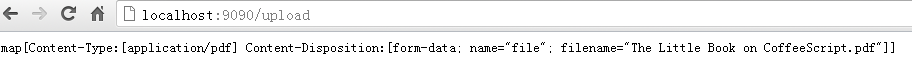
\includegraphics[width=14cm]{4.5.upload2.png}
   \label{図4.5}
   \caption{ファイルのアップロードを行った後サーバが受け取った情報の出力}
\end{figure}

\subsubsection{クライアントによるファイルのアップロード}
上の例でどのようにフォームからファイルをアップロードするのか示しました。その後サーバでファイルを処理しますが、Goは実はクライアントのフォームによるファイルのアップロードをエミュレートする機能をサポートしています。詳しい使用方法は以下の例をご覧ください:

\begin{lstlisting}[numbers=none]
package main

import (
    "bytes"
    "fmt"
    "io"
    "io/ioutil"
    "mime/multipart"
    "net/http"
    "os"
)

func postFile(filename string, targetUrl string) error {
    bodyBuf := &bytes.Buffer{}
    bodyWriter := multipart.NewWriter(bodyBuf)

    //キーとなる操作
    fileWriter, err := bodyWriter.CreateFormFile("uploadfile", filename)
    if err != nil {
        fmt.Println("error writing to buffer")
        return err
    }

    //ファイルハンドル操作をオープンする
    fh, err := os.Open(filename)
    if err != nil {
        fmt.Println("error opening file")
        return err
    }
    defer fh.Close()

    //iocopy
    _, err = io.Copy(fileWriter, fh)
    if err != nil {
        return err
    }

    contentType := bodyWriter.FormDataContentType()
    bodyWriter.Close()

    resp, err := http.Post(targetUrl, contentType, bodyBuf)
    if err != nil {
        return err
    }
    defer resp.Body.Close()
    resp_body, err := ioutil.ReadAll(resp.Body)
    if err != nil {
        return err
    }
    fmt.Println(resp.Status)
    fmt.Println(string(resp_body))
    return nil
}

// sample usage
func main() {
    target_url := "http://localhost:9090/upload"
    filename := "./astaxie.pdf"
    postFile(filename, target_url)
}
\end{lstlisting}

上の例ではクライアントが如何にサーバに対し一つのファイルをアップロードするのかご説明しました。クライアントはmultipart.Writeを通してファイルの本文をバッファの中に書き込みます。その後、httpのPostメソッドをコールしてバッファからサーバに転送します。

\begin{quote}
もしあなたが他にusernameといった普通のフィールドを同時に書き込む場合は、multipartのWriteFieldメソッドをコールして、その他の似たようなフィールドを複数書き込むことができます。
\end{quote}



\subsection{まとめ}
この一章ではGoでどのようにフォームの情報を処理するか学びました。ユーザのログインから、ファイルのアップロードの例で、Goがformの情報およびファイルをアップロードする手段についてご説明しました。しかしフォームを処理する過程ではユーザの入力した情報を検証する必要があります。ホームページのセキュリティの重要性を考慮すると、データのフィルタリングは相当重要です。そのため以降の章では異なる方面のデータフィルタリングをご説明します。同時にGoの文字列に対する正規表現についても述べます。

この一章を通してクライアントとサーバが如何にデータを互いにやりとりするか理解いただけたと思います。クライアントはデータをサーバシステムに渡し、サーバはデータを受け取って結果をクライアントにフィードバックします。



\section{データベースへのアクセス}
多くのWebアプリケーションプログラムにおいて、データベースはその核心となるものです。データベースはあなたが検索やさまざまな情報を修正したい場合にはほとんどで使用されます。例えばユーザ情報や製品の目録またはニュースのリスト等です。

Goはどのようなデータベースの使用もbuiltinではサポートされていません。しかし、Goはdatabase/sqlインターフェースを定義していますので、ユーザはこのドライバインターフェースに基いて目的のデータベースを使用することができます。5.1節でGoでデザインされているいくつかのドライバインターフェースやデータベースドライバインターフェースをご紹介します。5.2から5.4節では現在比較的使用されている関係型データドリブンとその使用方法についてご紹介します。5.5節では私が開発したORMライブラリをご紹介します。database/sqlの標準インターフェースに基づいた開発です。ほぼ全てのdatabase/sqlをサポートするデータベースの使用に互換性があります。Goスタイルで簡単にデータベース操作を行うことができます。

現在NOSQLはすでにWeb開発の流行となっています。多くのアプリケーションがNOSQLをデータベースとして採用しています。以前のキャッシュではありません。5.6節ではMongoDBとRedisの2つのNOSQLデータベースについてご紹介します。

\begin{quote}
Go database/sql tutorial(http://go-database-sql.org/)ではよく使われる例と詳細な説明を提供しています。
\end{quote}


\subsection{database/sqlインターフェース}
GoがPHPと異なる部分は、Goには公式に提供されたデータベースドライバがない事です。開発者が開発するためにデータベースドライバで標準のインターフェースが定義されています。開発者は定義されているインターフェースに従って目的のデータベースドライバを開発することができます。これにはメリットがあります。標準のインターフェースを参照するだけでコードを開発できます。以降データベースに移行する時、どのような修正も必要ありません。では、Goはどのような標準インターフェースを定義しているのでしょうか?詳しく分析してみることにしましょう。

\subsubsection{sql.Register}
database/sqlに存在する関数はデータベースドライバを登録するためにあります。サードパーティの開発者がデータベースドライバを開発する時は、すべてinit関数を実装します。init関数ではこの\texttt{Register(name string, driver driver.Driver)}をコールすることでこのドライバの登録を完了させます。

mymysql、sqlite3のドライバではどのようにコールしているのか見てみることにしましょう:

\begin{lstlisting}[numbers=none]
//https://github.com/mattn/go-sqlite3ドライバ
func init() {
    sql.Register("sqlite3", &SQLiteDriver{})
}

//https://github.com/mikespook/mymysqlドライバ
// Driver automatically registered in database/sql
var d = Driver{proto: "tcp", raddr: "127.0.0.1:3306"}
func init() {
    Register("SET NAMES utf8")
    sql.Register("mymysql", &d)
}
\end{lstlisting}

サードパーティのデータベースドライバはすべてこの関数をコールすることで自分のデータベースドライバの名前と目的のdriverを登録することがお分かりいただけたかと思います。database/sqlの内部ではひとつのmapを通してユーザが定義した目的のドライバを保存します。

\begin{lstlisting}[numbers=none]
var drivers = make(map[string]driver.Driver)

drivers[name] = driver
\end{lstlisting}

なぜならdatabase/sqlによって関数を登録できると同時に複数のデータベースドライバを登録することができるからです。重複させなければよいだけです。


\begin{quote}
database/sqlインターフェースとサードパーティライブラリを使用する時、よく以下のようになります:
\begin{lstlisting}[numbers=none]
import (
    "database/sql"
     _ "github.com/mattn/go-sqlite3"
)
\end{lstlisting}
新人はこの\texttt{\_}にとても戸惑いがちです。実はこれはGoの絶妙な設計なのです。変数に値を代入する際、よくこの記号が現れます。これは変数を代入する時のプレースホルダの省略です。パッケージのインポートにこの記号を使っても同じような作用があります。ここで使用した\texttt{\_}はインポートした後のパッケージ名で、このパッケージに定義されている関数、変数などのリソースを直接使用しない事を意味しています。

2.3節のフローと関数の章においてinit関数の初期化プロセスをご紹介しました。パッケージがインポートされる際はパッケージのinit関数が自動的にコールされ、このパッケージに対する初期化が完了します。そのため、上のデータベースドライバパッケージをインポートするとinit関数が自動的にコールされます。つぎに、init関数でこのデータベースドライバを登録し、以降のコードの中で直接このデータベースドライバを直接使用することができます。
\end{quote}

\subsubsection{driver.Driver}
Driverはデータベースドライバのインターフェースです。methodがひとつ定義されています: Open(name string)、このメソッドはデータベースのConnインターフェースを一つ返します。

\begin{lstlisting}[numbers=none]
type Driver interface {
    Open(name string) (Conn, error)
}
\end{lstlisting}

返されるConnは一回のgoroutineの操作を行う事ができるだけです。このConnをGoの複数のgoroutineの中に使うことはできません。以下のコードはエラーが発生します。

\begin{lstlisting}[numbers=none]
...
go goroutineA (Conn)  //検索操作の実行
go goroutineB (Conn)  //挿入操作の実行
...

\end{lstlisting}

上のようなコードではGoにとってどのような操作がどのgoroutineによって行われたのか知り得ませんのでデータの混乱を招きます。たとえばgoroutineAで実行された検索操作の結果をgoroutineBに返す場合Bはこの結果を自分が実行した挿入データだと誤解してしまいます。

サードパーティドライバはすべてこの関数を定義しています。これはname引数を解析することによって目的のデータベースの接続情報を得ることができます。解析が終わると、この情報を使って、ひとつのConnを初期化し、それを返します。



\subsubsection{driver.Conn}
Connはデータベース接続のインターフェース定義です。これにはいくつかのメソッドが定義されています。このConnはひとつのgoroutineの中でしか使用することができず、複数のgoroutineの中では使用することができません。詳細は上の説明をご確認ください。

\begin{lstlisting}[numbers=none]
type Conn interface {
    Prepare(query string) (Stmt, error)
    Close() error
    Begin() (Tx, error)
}
\end{lstlisting}

Prepare関数は現在の接続と関連した実行されるSQL文の準備状態を返します。検索、削除等の操作を行うことができます。

Close関数は現在の接続を閉じます。接続が持っているリソースを開放するなど整理作業を行います。ドライバはdatabase/sqlの中のconn poolを実現しているので、問題を起こしやすいのです。

Begin関数はトランザクション処理を表すTxを返します。これを利用して検索、更新といった操作を行うことができます。またはトランザクションに対してロールバックやコミットを行います。


\subsubsection{driver.Stmt}
Stmtは準備が整った状態です。Connの関連性と、またひとつのgoroutineの中でしか使用することができません。複数のgoroutineに使用することはできません。

\begin{lstlisting}[numbers=none]
type Stmt interface {
    Close() error
    NumInput() int
    Exec(args []Value) (Result, error)
    Query(args []Value) (Rows, error)
}
\end{lstlisting}

Close関数は現在の接続状態を閉じます。ただし、もし現在実行されているqueryはrowsデータを返します。

NumInput関数は現在予約されている引数の個数を返します。$>$=0が返された時はデータベースドライバがインテリジェントに使用側の引数を検査します。データベースドライバパッケージが予約された引数を知らない場合は-1を返します。

Exec関数はPrepareで準備の整ったsqlを実行します。引数を渡し、update/insertといった操作を実行します。Resultデータを返します。

Query関数はPrepareで準備の整ったsqlを実行します。必要な引数を渡し、select操作を実行します。Rowsリザルトセットを返します。


\subsubsection{driver.Tx}
トランザクション処理には一般的に2つのプロセスがあります。コミットかロールバックです。データベースドライバの中ではこの2つの関数を実装すれば問題ありません。

\begin{lstlisting}[numbers=none]
type Tx interface {
    Commit() error
    Rollback() error
}
\end{lstlisting}

この2つの関数のうちひとつはコミットに使用され、もうひとつはロールバックに使用されます。

\subsubsection{driver.Execer}
これはConnが実装できるインターフェースです。

\begin{lstlisting}[numbers=none]
type Execer interface {
    Exec(query string, args []Value) (Result, error)
}
\end{lstlisting}

もしこのインターフェースの定義がなければ、DB.Execがコールされます。つまり、まずPrepareがコールされStmtを返し、その後StmtのExecが実行され、Stmtが閉じられます。

\subsubsection{driver.Result}
これはUpdate/Insertといった操作が行った結果を返すインターフェースの定義です。

\begin{lstlisting}[numbers=none]
type Result interface {
    LastInsertId() (int64, error)
    RowsAffected() (int64, error)
}
\end{lstlisting}

LastInsertId関数はデータベースによって実行された挿入操作によって得られるインクリメントIDを返します。

RowsAffected関数はquery操作で影響されるデータの数を返します。

\subsubsection{driver.Rows}
Rowsは実行された検索のリザルトセットのインターフェースの定義です

\begin{lstlisting}[numbers=none]
type Rows interface {
    Columns() []string
    Close() error
    Next(dest []Value) error
}
\end{lstlisting}

Columns関数はデータベースの検索におけるフィールド情報を返します。これが返すsliceとsql検索のフィールドは一つ一つが対応しており、すべての表のフィールドを返すわけではありません。

Close関数はRowsイテレータを閉じるために用いられます。

Next関数はひとつのデータを返すのに用いられます。データはdestに代入され、destの中の要素はstringを除いてdriver.Valueの値でなければなりません。返されるデータの中のすべてのstringは[]byteに変換される必要があります。もし最後にデータが無い場合、Next関数はio.EOFを返します。

\subsubsection{driver.RowsAffected}
RowsAffectedは実はint64のエイリアスです。しかしResultインターフェースを実装していますので、低レイヤーでResultの表示メソッドを実装するために用いられます。

\begin{lstlisting}[numbers=none]
type RowsAffected int64

func (RowsAffected) LastInsertId() (int64, error)

func (v RowsAffected) RowsAffected() (int64, error)
\end{lstlisting}

\subsubsection{driver.Value}
Valueは実は空のインターフェースです。どのようなデータも格納することができます。

\begin{lstlisting}[numbers=none]
type Value interface{}
\end{lstlisting}

driveのValueはドライバが必ず操作できるValueです。Valueがnilでなければ、下のいずれかとなります

\begin{lstlisting}[numbers=none]
int64
float64
bool
[]byte
string   [*]Rows.Nextが返すものを除いてstringではありません。
time.Time
\end{lstlisting}

\subsubsection{driver.ValueConverter}
ValueConverterインターフェースはどのように普通の値をdriver.Valueのインターフェースの変換するか定義されています。

\begin{lstlisting}[numbers=none]
  type ValueConverter interface {
    ConvertValue(v interface{}) (Value, error)
  }
\end{lstlisting}

開発しているデータベースドライバパッケージではこのインターフェースの関数が多くの場所で利用されています。このValueConverterにはメリットがたくさんあります:

\begin{itemize}
\item driver.valueはデータベース表の対応するフィールドに特化されています。たとえばint64のデータがどのようにデータベース表のunit16フィールドに変換されるかといったことです。
\item データベースの検索結果をdriver.Value値に変換します。
\item scan関数ではどのようにしてdriver.Valueの値をユーザが定義した値に変換するか
\end{itemize}

\subsubsection{driver.Valuer}
Valueインターフェースではdriver.Valueをひとつ返すメソッドが定義されています。

\begin{lstlisting}[numbers=none]
type Valuer interface {
    Value() (Value, error)
}
\end{lstlisting}

たくさんの型がこのValueメソッドを実装しています。自分自身とdriver.Valueに特化して利用されます。 

上の説明によって、ドライバの開発について基本的なことがお分かりいただけたかとおもいます。このドライバはただこれらインターフェースを実装して追加・削除・検索・修正といった基本操作を可能にするだけです。あとは対応するデータベースに対してデータをやりとりするなど細かい問題が残っています。ここでは細かく述べることはしません。

\subsubsection{database/sql}
database/sqlではdatabase/sql/driverにて提供されるインターフェースの基礎の上にいくつかもっと高い階層のメソッドを定義しています。データベース操作を容易にし、内部でconn poolを実装しています。

\begin{lstlisting}[numbers=none]
type DB struct {
    driver      driver.Driver
    dsn         string
    mu       sync.Mutex // protects freeConn and closed
    freeConn []driver.Conn
    closed   bool
}
\end{lstlisting}

Open関数がDBオブジェクトを返しています。この中にはfreeConnがあり、これがまさに簡単な接続プールのことです。この実装はとても簡単でまた簡素です。Db.prepareを実行する際\texttt{defer db.putConn(ci, err)}を行います。つまりこの接続を接続プールに放り込むのです。毎回connをコールする際はまずfreeConnの長さが0よりも大きいか確認し、0よりも大きかった場合connを再利用してもよいことを示しています。直接使ってかまいません。もし0以下であった場合はconnを作成してこれを返します。


\subsection{MySQL データベースの使用}
現在Internet上で流行しているホームページフレームワークの方法はLAMPです。この中のMがMySQLです。データベースとして、MySQLは無料、オープンソース、使用方法において多くのWeb開発のバックエンドのデータベースストレージエンジンとして優位に立ってきました。

\subsubsection{MySQLドライバ}
GoではMySQLをサポートしたドライバが現在比較的多く、以下のようにいくつかが存在します。あるものはdatabase/sql標準をサポートしており、またあるものは独自でインターフェースの実装を採用しているものもあります。よく使われるものは以下のいくつかです:

\begin{description}
  \item[https://github.com/go-sql-driver/mysql] database/sqlをサポートしており、すべてgoで書かれています。
  \item[https://github.com/ziutek/mymysql] database/sqlをサポートしており、独自に定義されたインターフェースもサポートしています。すべてgoで書かれています。
  \item[https://github.com/Philio/GoMySQL] database/sqlをサポートしていません。独自のインターフェースで、すべてgoで書かれています。
\end{description}

以降の例では私ははじめのドライバを使ってまいります。(現在の項目でもこのドライバを使います)、またこのドライバの利用をみなさんにお勧めします。理由は:

\begin{itemize}
  \item このドライバは比較的新しく、メンテナンスも良いほうです。
  \item 完全にdatabase/sqlインターフェースをサポートします。
  \item keepaliveをサポートしています。継続した接続を保持しています。星星(http://www.mikespook.com/)がforkしたmymysqlもkeepaliveをサポートしているとはいえ、スレッドセーフではありません。これは低いレイヤーからkeepaliveをサポートしています。
\end{itemize}


\subsubsection{コード例}
続くいくつかの節では同じデータベーススキーマを採用します:データベースtest、ユーザ名userinfo、関連ユーザ情報テーブルuserdetail。

\begin{lstlisting}[numbers=none]
CREATE TABLE `userinfo` (
    `uid` INT(10) NOT NULL AUTO_INCREMENT,
    `username` VARCHAR(64) NULL DEFAULT NULL,
    `departname` VARCHAR(64) NULL DEFAULT NULL,
    `created` DATE NULL DEFAULT NULL,
    PRIMARY KEY (`uid`)
)

CREATE TABLE `userdetail` (
    `uid` INT(10) NOT NULL DEFAULT '0',
    `intro` TEXT NULL,
    `profile` TEXT NULL,
    PRIMARY KEY (`uid`)
)
\end{lstlisting}

以下の例ではどのようにしてdatabase/sqlインターフェースを使ってデータベースのテーブルに対し、追加・削除・修正・検索操作を行うか示しています。

\begin{lstlisting}[numbers=none]
package main

import (
    _ "github.com/go-sql-driver/mysql"
    "database/sql"
    "fmt"
    //"time"
)

func main() {
    db, err := sql.Open("mysql",
                        "astaxie:astaxie@/test?charset=utf8")
    checkErr(err)

    //データの挿入
    stmt, err := db.Prepare(
       "INSERT userinfo SET username=?,departname=?,created=?")
    checkErr(err)

    res, err := stmt.Exec("astaxie", "研究開発部門", "2012-12-09")
    checkErr(err)

    id, err := res.LastInsertId()
    checkErr(err)

    fmt.Println(id)
    //データの更新
    stmt, err = db.Prepare("update userinfo set username=? where uid=?")
    checkErr(err)

    res, err = stmt.Exec("astaxieupdate", id)
    checkErr(err)

    affect, err := res.RowsAffected()
    checkErr(err)

    fmt.Println(affect)

    //データの検索
    rows, err := db.Query("SELECT * FROM userinfo")
    checkErr(err)

    for rows.Next() {
        var uid int
        var username string
        var department string
        var created string
        err = rows.Scan(&uid, &username, &department, &created)
        checkErr(err)
        fmt.Println(uid)
        fmt.Println(username)
        fmt.Println(department)
        fmt.Println(created)
    }

    //データの削除
    stmt, err = db.Prepare("delete from userinfo where uid=?")
    checkErr(err)

    res, err = stmt.Exec(id)
    checkErr(err)

    affect, err = res.RowsAffected()
    checkErr(err)

    fmt.Println(affect)

    db.Close()

}

func checkErr(err error) {
    if err != nil {
        panic(err)
    }
}
\end{lstlisting}

上のコードで、GoがMysqlデータベースを操作するのが非常に簡単だとお分かりいただけたかと思います。

キーとなるいくつかの関数についてご説明します:

sql.Open()関数は登録済みのデータベースドライバを開くために使用されます。go-sql-driverの中でmysqlのデータベースドライバを登録し、2つ目の引数はDSN(Data Source Name)です。これはgo-sql-driverが定義するデータベース接続と設定情報です。以下のシンタックスをサポートします:

\begin{lstlisting}[numbers=none]
user@unix(/path/to/socket)/dbname?charset=utf8
user:password@tcp(localhost:5555)/dbname?charset=utf8
user:password@/dbname
user:password@tcp([de:ad:be:ef::ca:fe]:80)/dbname
\end{lstlisting}

db.Prepare()関数はsql操作を実行するプリペアードステートメントを返すために用いられます。その後、準備完了の実行状態を返します。

db.Query()関数は直接Sqlを実行しRows結果を返すために使われます。

stmt.Exec()関数はstmtが用意されたSQL文を実行するために用いられます。

渡される引数がどれも=?に対応するデータであることがわかるかとおもいます。このような方法である程度SQLインジェクションを防止することができます。



\subsection{SQLiteデータベースの使用}
SQLiteはオープンソースの組み込み式リレーショナルデータベースです。独立しており、設定なしでトランザクションのSQLデータベースエンジンをサポートします。非常にポータブルで簡単に利用でき、コンパクトで効率が高く、信頼性があります。他のデータベース管理システムとは異なり、SQLiteのインストールと実行は非常に簡単です。多くの場合は、ただSQLiteのバイナリファイルを用意するだけですぐに作成、接続、使用することができます。もしあなたが現在組み込み式データベースかソリューションをお探しであれば、SQLiteは絶対に考慮するに値します。SQLiteはいわばオープンソースのAccessのようなものです。

\subsubsection{ドライバ}
Goがサポートするsqliteのドライバも比較的多いのですが、大部分はdatabase/sqlインターフェースをサポートしていません。

\begin{description}
  \item[https://github.com/mattn/go-sqlite3] database/sqlインターフェースをサポートしています。cgo(cgoに関する情報はオフィシャルドキュメントかこの本の最後の章をご参考ください)に基づいて記述されています。
  \item[https://github.com/feyeleanor/gosqlite3] database/sqlインターフェースをサポートしていません。cgoに基いて記述されています。
  \item[https://github.com/phf/go-sqlite3] database/sqlインターフェースをサポートしていません。cgoに基いて記述されています。
\end{description}

現在database/sqlをサポートしているSQLiteデータベースドライバは一つ目だけです。私も現在これを採用してプロジェクトで開発しています。標準インターフェースを採用することは今後より良いドライバが開発された時に移行できることです。

\subsubsection{実例コード}
例に示すデータベーススキーマは以下の通りです。対応するテーブル作成SQL:

\begin{lstlisting}[numbers=none]
CREATE TABLE `userinfo` (
    `uid` INTEGER PRIMARY KEY AUTOINCREMENT,
    `username` VARCHAR(64) NULL,
    `departname` VARCHAR(64) NULL,
    `created` DATE NULL
);

CREATE TABLE `userdeatail` (
    `uid` INT(10) NULL,
    `intro` TEXT NULL,
    `profile` TEXT NULL,
    PRIMARY KEY (`uid`)
);
\end{lstlisting}

下のGoプログラムがどのようにデータベースのテーブルのデータを操作するか見てみましょう:追加・削除・修正・検索

\begin{lstlisting}[numbers=none]
package main

import (
    "database/sql"
    "fmt"
    "time"
    _ "github.com/mattn/go-sqlite3"
)

func main() {
    db, err := sql.Open("sqlite3", "./foo.db")
    checkErr(err)

    //データの挿入
    stmt, err := db.Prepare("INSERT INTO userinfo(username,
                             departname, created) values(?,?,?)")
    checkErr(err)

    res, err := stmt.Exec("astaxie", "研究開発部門", "2012-12-09")
    checkErr(err)

    id, err := res.LastInsertId()
    checkErr(err)

    fmt.Println(id)
    //データの更新
    stmt, err = db.Prepare("update userinfo set username=? where uid=?")
    checkErr(err)

    res, err = stmt.Exec("astaxieupdate", id)
    checkErr(err)

    affect, err := res.RowsAffected()
    checkErr(err)

    fmt.Println(affect)

    //データの検索
    rows, err := db.Query("SELECT * FROM userinfo")
    checkErr(err)

    for rows.Next() {
        var uid int
        var username string
        var department string
        var created time.Time
        err = rows.Scan(&uid, &username, &department, &created)
        checkErr(err)
        fmt.Println(uid)
        fmt.Println(username)
        fmt.Println(department)
        fmt.Println(created)
    }

    //データの削除
    stmt, err = db.Prepare("delete from userinfo where uid=?")
    checkErr(err)

    res, err = stmt.Exec(id)
    checkErr(err)

    affect, err = res.RowsAffected()
    checkErr(err)

    fmt.Println(affect)

    db.Close()

}

func checkErr(err error) {
    if err != nil {
        panic(err)
    }
}
\end{lstlisting}

上のコードとMySQLの例の中のコードはほとんどまったく同じです。唯一異なるのはドライバのインポート部分です。\texttt{sql.Open}のコールではSQLiteの方法で開きます。

\begin{quote}
sqlite管理ツール:http://sqliteadmin.orbmu2k.de/

簡単にデータベース管理を新規作成することができます。
\end{quote}




\subsection{PostgreSQLデータベースの使用}
PostgreSQLはフリーなオブジェクト-リレーショナルデータベースサーバ(データベース管理システム)です。これは活発なBSDライクなライセンスで公開されています。他のオープンソースなデータベースシステム(MySQLやFirebird)やOracle、Sybase、IBMのDB2やMicrosoft SQL Serverといったプロプライエタリなシステムに対する選択肢の一つです。

PostgreSQLとMySQLを比較すると、これは少々巨大です。これはOracleの代替として設計されているためです。そのため、企業のアプリケーションではPostgreSQLを選択することが賢い選択の一つとなっています。

MySQLはOracleに買収され、現在徐々にクローズされつつあります。(MySQL 5.5.31以降のすべてのバージョンがGPLライセンスを順守していません)。これに鑑み、将来我々もプロジェクトのバックエンドのデータベースとしてMySQLではなくPostgreSQLを選択することになるかもしれません。

\subsubsection{ドライバ}
GoはPostgreSQLをサポートしたドライバも非常に多く実装されています。国外では多くの人が開発でこのデータベースを使用しているためです。

\begin{description}
  \item[https://github.com/lib/pq] database/sqlドライバをサポートしています。純粋にGoで書かれています。
  \item[https://github.com/jbarham/gopgsqldriver] database/sqlドライバをサポートしています。純粋にGoで書かれています。
  \item[https://github.com/lxn/go-pgsql] database/sqlドライバをサポートしています。純粋にGoで書かれています。
\end{description}

下の例では一つ目のドライバを採用してご説明します。これは使用している人が最も多く、githubでも比較的活発であるからです。

\subsubsection{実例コード}
データベースのテーブル作成文:


\begin{lstlisting}[numbers=none]
CREATE TABLE userinfo
(
    uid serial NOT NULL,
    username character varying(100) NOT NULL,
    departname character varying(500) NOT NULL,
    Created date,
    CONSTRAINT userinfo_pkey PRIMARY KEY (uid)
)
WITH (OIDS=FALSE);

CREATE TABLE userdeatail
(
    uid integer,
    intro character varying(100),
    profile character varying(100)
)
WITH(OIDS=FALSE);
\end{lstlisting}

下ではGoがどのようにデータベースのテーブルのデータを操作するか見て行きましょう:追加・削除・修正・検索

\begin{lstlisting}[numbers=none]
package main

import (
    "database/sql"
    "fmt"
    _ "https://github.com/lib/pq"
)

func main() {
    db, err := sql.Open("postgres", "user=astaxie password=astaxie
                         dbname=test sslmode=disable")
    checkErr(err)

    //データの挿入
    stmt, err := db.Prepare("INSERT INTO userinfo(username,departname,
                              created) VALUES($1,$2,$3) RETURNING uid")
    checkErr(err)

    res, err := stmt.Exec("astaxie", "研究開発部門", "2012-12-09")
    checkErr(err)

    //pgはこの関数をサポートしていません。
    //MySQLのインクリメンタルなIDのようなものが無いためです。
    id, err := res.LastInsertId()
    checkErr(err)

    fmt.Println(id)

    //データの更新
    stmt, err = db.Prepare("update userinfo set username=$1 where
                                                          uid=$2")
    checkErr(err)

    res, err = stmt.Exec("astaxieupdate", 1)
    checkErr(err)

    affect, err := res.RowsAffected()
    checkErr(err)

    fmt.Println(affect)

    //データの検索
    rows, err := db.Query("SELECT * FROM userinfo")
    checkErr(err)

    for rows.Next() {
        var uid int
        var username string
        var department string
        var created string
        err = rows.Scan(&uid, &username, &department, &created)
        checkErr(err)
        fmt.Println(uid)
        fmt.Println(username)
        fmt.Println(department)
        fmt.Println(created)
    }

    //データの削除
    stmt, err = db.Prepare("delete from userinfo where uid=$1")
    checkErr(err)

    res, err = stmt.Exec(1)
    checkErr(err)

    affect, err = res.RowsAffected()
    checkErr(err)

    fmt.Println(affect)

    db.Close()

}

func checkErr(err error) {
    if err != nil {
        panic(err)
    }
}
\end{lstlisting}

上のコードによって、PostgreSQLが\texttt{\$1}や\texttt{\$2}といった方法によって引数を渡している様子がお分かりいただけるかとおもいます。MySQLの中の\texttt{?}ではありません。また、sql.Openではdsn情報のシンタックスがMySQLのドライバでのdsnシンタックスと異なります。そのため、使用される際はこの違いにご注意ください。

また、pgはLastInsertId関数をサポートしていません。PostgreSQLの内部ではMySQLのインクリメンタルなIDを返すといった実装がないためです。その他のコードはほとんど同じです。


\subsection{beedbライブラリを使用してORM開発を行う}
beedbは私が開発したGoによるORM操作のためのライブラリです。これはGo styleの方法でデータベースに対し操作を行います。structからテーブルの記録へのマッピングを実現します。beedbは十分軽量なGo ORMフレームワークです。このライブラリを開発した動機は複雑なORM学習曲線を引き下げたいと思ったからです。出来る限りORMの実行効率と機能の間でバランスをとったつもりです。beedbは現在オープンソースのGo ORMフレームワークの中で比較的完全なライブラリのひとつです。また、実行効率も相当良く、機能も基本的に需要を満足させています。しかし現在はまだアソシエーション関係をサポートしておらず、これは次のバージョンの主なポイントです。

beedbはdatabase/sql標準インターフェースをサポートしたORMライブラリです。そのため、理論上では、データベースドライバがdatabase/sqlインターフェースをサポートしていさえすればすんなりbeedbを使うことができます。現在までに私がテストしたドライバパッケージは以下のとおり:

\begin{description}
  \item Mysql:github.com/ziutek/mymysql/godrv[*]
  \item Mysql:github/go-mysql-driver/mysql[*]
  \item PostgreSQL:github.com/lib/pq[*]
  \item SQLite:github.com/mattn/go-sqlite3[*]
  \item MS ADODB: github.com/mattn/go-adodb[*]
  \item ODBC: bitbucket.org/miquella/mgodbc[*]
\end{description}

\subsubsection{インストール}
beedbはgo get方式によるインストールをサポートしています。これはGo Styleの方式に完全に則って実装されています。

\begin{lstlisting}[numbers=none]
go get github.com/astaxie/beedb
\end{lstlisting}

\subsubsection{初期化の方法}
まず対応するデータベースドライバパッケージをimportする必要があります。database/sql標準インターフェースパッケージおよびbeedbパッケージです:

\begin{lstlisting}[numbers=none]
import (
    "database/sql"
    "github.com/astaxie/beedb"
    _ "github.com/ziutek/mymysql/godrv"
)
\end{lstlisting}

必要なパッケージをインポートした後、データベースへの接続を開く必要があります。その後beedbオブジェクト(たとえばMySQLとします)を作成します


\begin{lstlisting}[numbers=none]
db, err := sql.Open("mymysql", "test/xiemengjun/123456")
if err != nil {
    panic(err)
}
orm := beedb.New(db)
\end{lstlisting}

beedbのNew関数は2つの引数を必要とします。一つ目の引数は標準インターフェースのdbで、二つ目の引数は利用するデータベースエンジンです。もしあなたが使用するデータベースエンジンがMySQL/Sqliteだった場合、二つ目の引数は省略してもかまいません。

もしSQLServerをお使いであれば、このように初期化する必要があります:

\begin{lstlisting}[numbers=none]
orm = beedb.New(db, "mssql")
\end{lstlisting}

もしPostgreSQLをお使いであれば、初期化は以下のようになります:

\begin{lstlisting}[numbers=none]
orm = beedb.New(db, "pg")
\end{lstlisting}

現在beedbはプリントデバッグをサポートしていますので、下のコードでデバッグを行うことができます。

\begin{lstlisting}[numbers=none]
beedb.OnDebug=true
\end{lstlisting}

以降の例では前のデータベースのテーブルUserinfoを採用します。まず目的のstructを作成します。

\begin{lstlisting}[numbers=none]
type Userinfo struct {
    Uid     int `PK` //もしテーブルのプライマリキーがidで
                     //なければ、pkコメントを追加する必要が
                     //あります。このフィールドがプライマリ
                     //キーであることを明示します。
    Username    string
    Departname  string
    Created     time.Time
}
\end{lstlisting}

\begin{quote}
ご注意ください。beedbはキャメルケースの命名規則を自動でスネークケースのフィールドに変換します。たとえば\texttt{UserInfo}という名前のStructを定義した場合、低レイヤで実装される際に\texttt{user\_info}と変換されます。フィールドの命名もこのルールに従います。
\end{quote}

\subsubsection{データの挿入}
下のコードはどのように記録を挿入するか示しています。我々が操作しているのはstructオブジェクトで、元々のsql文ではありません。Saveインターフェースをコールしてデータをデータベースに保存します。

\begin{lstlisting}[numbers=none]
var saveone Userinfo
saveone.Username = "Test Add User"
saveone.Departname = "Test Add Departname"
saveone.Created = time.Now()
orm.Save(&saveone)
\end{lstlisting}

挿入後、挿入に成功した際のインクリメンタルなIDが\texttt{saveone.Uid}です。Saveインターフェースは自動的に保存します。

beedbインターフェースはもう一種類の挿入の方法を提供しています。mapデータ挿入です。

\begin{lstlisting}[numbers=none]
add := make(map[string]interface{})
add["username"] = "astaxie"
add["departname"] = "cloud develop"
add["created"] = "2012-12-02"
orm.SetTable("userinfo").Insert(add)
\end{lstlisting}

複数のデータを挿入

\begin{lstlisting}[numbers=none]
addslice := make([]map[string]interface{}, 0)
add:=make(map[string]interface{})
add2:=make(map[string]interface{})
add["username"] = "astaxie"
add["departname"] = "cloud develop"
add["created"] = "2012-12-02"
add2["username"] = "astaxie2"
add2["departname"] = "cloud develop2"
add2["created"] = "2012-12-02"
addslice =append(addslice, add, add2)
orm.SetTable("userinfo").InsertBatch(addslice)
\end{lstlisting}

上の操作方法はメソッドチェーンによる検索にすこし似ています。jqueryに詳しい方はとても馴染みがあるのではないでしょうか。毎回コールされるmethodはすべてもともとのormオブジェクトを返しているので、継続してオブジェクトの他のmethodをコールすることができます。

上でコールしたSetTable関数はORMに対して、これから実行するこのmapに対応したデータベーステーブルが\texttt{userinfo}であると明示しています。

\subsubsection{データの更新}
つづけて上の例で更新操作をご覧にいれましょう。現在saveoneのプライマリキーはすでに値が存在します。この時saveインターフェースをコールして、beedb内は自動的にupdateをコールすることによってデータの更新を行います。挿入操作ではありません。

\begin{lstlisting}[numbers=none]
saveone.Username = "Update Username"
saveone.Departname = "Update Departname"
saveone.Created = time.Now()
orm.Save(&saveone)  //現在saveoneにはプライマリキーが
                    //あります。更新操作を行います。
\end{lstlisting}

データの更新はmap操作の直接の使用をサポートしています。

\begin{lstlisting}[numbers=none]
t := make(map[string]interface{})
t["username"] = "astaxie"
orm.SetTable("userinfo").SetPK("uid").Where(2).Update(t)
\end{lstlisting}

ここではいくつかのbeedbの関数をコールしてみます。

SetPK:ORMに対して、データベースのテーブル\texttt{userinfo}のプライマリキーがuidであることを明示します。

Where:条件を設定するために用いられます。複数の引数をサポートし、第一引数がもし整数であった場合、Where("プライマリキー=?",値)がコールされたものとなります。 Update関数はmap型のデータを受け取り、データの更新を実行します。


\subsubsection{データの検索}
beedbの検索インターフェースは使いやすく、具体的な使用方法は下の例をご覧ください。

例1、プライマリキーによってデータを取得:

\begin{lstlisting}[numbers=none]
var user Userinfo
//Whereは2つの引数を受け取ります。int型の引数をサポートします。
orm.Where("uid=?", 27).Find(&user)
\end{lstlisting}

例2:

\begin{lstlisting}[numbers=none]
var user2 Userinfo
orm.Where(3).Find(&user2) // これは上の省略版です。
                          //プライマリキーは省略できます。
\end{lstlisting}

例3、プライマリキーではない条件:

\begin{lstlisting}[numbers=none]
var user3 Userinfo
//Whereは2つの引数を受け取ります。文字列型の引数をサポートします。
orm.Where("name     = ?", "john").Find(&user3)
\end{lstlisting}

例4、もっと複雑な条件:

\begin{lstlisting}[numbers=none]
var user4 Userinfo
//Whereは3つの引数をサポートします。
orm.Where("name = ? and age < ?", "john", 88).Find(&user4)
\end{lstlisting}

下のインターフェースを通して複数のデータを取得できます。例をご覧ください。

例1、条件id$>$3にもとづいて、20からはじまる10件のデータを取得します。


\begin{lstlisting}[numbers=none]
var allusers []Userinfo
err := orm.Where("id > ?", "3").Limit(10,20).FindAll(&allusers)
\end{lstlisting}

例2、limitの第二引数は省略できます。デフォルトは0から開始となります。10件のデータを取得します。

\begin{lstlisting}[numbers=none]
var tenusers []Userinfo
err := orm.Where("id > ?", "3").Limit(10).FindAll(&tenusers)
\end{lstlisting}

例3、すべてのデータを取得します。

\begin{lstlisting}[numbers=none]
var everyone []Userinfo
err := orm.OrderBy("uid desc,username asc").FindAll(&everyone)
\end{lstlisting}

上ではLimit関数があります。これは検索結果の数をコントロールするのに用いられます。

Limit:2つの引数をサポートします。第一引数は検索数を表し、第二引数は取得するデータの開始位置を表しています。デフォルトは0です。

OrderBy:この関数は検索をソートするために用いられます。引数はソートの条件である必要があります。

上の例では取得するデータが直接structオブジェクトにマッピングされます。もし、データをmapとして取得したいだけであれば、下の方法で実現することができます:

\begin{lstlisting}[numbers=none]
a, _ := orm.SetTable("userinfo").SetPK("uid").
            Where(2).Select("uid,username").FindMap()
\end{lstlisting}

上とこの例の中ではまた新しいインターフェースの関数Selectがでてきました。この関数はいくつのフィールドを検索したいのか定義するために用いられます。デフォルトでは全てのフィールドとなる\texttt{*}となります。

FindMap()関数は\texttt{[]map[string][]byte}型を返します。そのため、自分自身で型変換を行う必要があります。

\subsubsection{データの削除}
beedbは豊富なデータ削除インターフェースを備えています。下の例をご覧ください。

例1、単一のデータを削除

\begin{lstlisting}[numbers=none]
//saveoneは上の例で示したあのsaveoneです。
orm.Delete(&saveone)
\end{lstlisting}

例2、複数のデータを削除

\begin{lstlisting}[numbers=none]
//alluserは上で定義した複数のデータのsliceです。
orm.DeleteAll(&alluser)
\end{lstlisting}

例3、sqlにしたがってデータを削除

\begin{lstlisting}[numbers=none]
orm.SetTable("userinfo").Where("uid>?", 3).DeleteRow()
\end{lstlisting}



\subsubsection{リレーション検索}
現在beedbはstructのリレーションをサポートしていません。しかしいくつかのアプリケーションはリレーションによる検索を必要としています。そのため、現在beedbは簡単なソリューションを提供しています。

\begin{lstlisting}[numbers=none]
a, _ := orm.SetTable("userinfo").
        Join("LEFT", "userdeatail", "userinfo.uid=userdeatail.uid").
        Where("userinfo.uid=?", 1).
        Select("userinfo.uid,userinfo.username,userdeatail.profile").
        FindMap()
\end{lstlisting}


上のコードでは新しいインターフェースのJoin関数が出て来ました。この関数には3つの引数があります。

\begin{itemize}
  \item 第一引数には:INNER, LEFT, OURTER, CROSS等が入れられます
  \item 第二匹数は接続するテーブルを表します
  \item 第三引数は接続の条件を表します
\end{itemize}

\subsubsection{Group ByとHaving}
いくつかのアプリケーションがgroup byとhavingの機能を必要としているため、beedbも簡単な実現方法を提供しています。


\begin{lstlisting}[numbers=none]
a, _ := orm.SetTable("userinfo").
            GroupBy("username").
            Having("username='astaxie'").
            FindMap()
\end{lstlisting}

上のコードで現れる2つの新しいインターフェースの関数

GroupBy:groupbyのフィールドを実行するために用いられます

Having:havingを実行する際の条件を指定するために用いられます


\subsubsection{一歩進んで}
現在beedbはすでに多くの国内外からのユーザによってフィードバックを得ています。現在作り直しを考えています。以降ではいくつかの方面で改良が行われる予定です。

\begin{itemize}
  \item interface設計の実装。database/sql/driverの設計に似て、beedbのインターフェースを設計します。その後対応するデータベースのCRUD操作を実現します。
  \item リレーショナルデータベースの設計の実現。一対一、一対多、多対多のサポートを実現します。コードは以下のとおり:
\begin{lstlisting}[numbers=none]
type Profile struct{
    Nickname    string
    Mobile        string
}

type Userinfo struct {
    Uid     int `PK`
    Username    string
    Departname  string
    Created     time.Time
    Profile     `HasOne`
}
\end{lstlisting}
  \item 自動的にデータベース、テーブル、インデックスを作成
  \item 接続プールの実現、goroutineを採用。
\end{itemize}


\subsection{NOSQLデータベースの操作}
NoSQL(Not Only SQL)とは、リレーション型ではないデータベースのことを言います。Web2.0の高まりにしたがって、伝統的なリレーショナルデータベースがWeb2.0ページに使われています。特にとても大きな規模で高度にマルチスレッドなSNS型のWeb2.0の純粋な動的ホームページでは明らかに力不足となっています。多くの解決が難しい問題が暴露され、リレーショナルでないデータベースはその特徴から非常に早く発展してきています。

Go言語は21世紀のC言語として、NOSQLもとてもよくサポートしています。現在流行しているNOSQLには主にredis、mongoDB、CassandraとMembase等があります。これらのデータベースはどれも高性能、マルチスレッドといった特徴があり、現在すでに広くあらゆるアプリケーションの中で使用されています。ここでは主にredisとmongoDBの操作についてご説明します。



\subsubsection{redis}
redisはkey-valueを保存するシステムです。Memcachedに似ていて、保存されるvalue型はもっと多く、string(文字列)、list(リスト)、set(集合)とzset(順序付きset)を含みます。

現在redisが最もよく使われているのは新浪のマイクロブログプラットフォームでしょう。その次にFacebookに買収された画像フォーラムであるinstagramがあります。その他有名なインターネット企業もそうです。

Goは現在redisのドライバで以下をサポートしています

\begin{itemize}
  \item https://github.com/garyburd/redigo
  \item https://github.com/go-redis/redis
  \item https://github.com/hoisie/redis
  \item https://github.com/alphazero/Go-Redis
  \item https://github.com/simonz05/godis
\end{itemize}

redigoのドライバを使ってデータベースを操作する方法を見てみましょう:

\begin{lstlisting}[numbers=none]
package main

import (
    "fmt"
    "github.com/garyburd/redigo/redis"
    "os"
    "os/signal"
    "syscall"
    "time"
)

var (
    Pool *redis.Pool
)

func init() {
    redisHost := ":6379"
    Pool = newPool(redisHost)
    close()
}

func newPool(server string) *redis.Pool {

    return &redis.Pool{

        MaxIdle:     3,
        IdleTimeout: 240 * time.Second,

        Dial: func() (redis.Conn, error) {
            c, err := redis.Dial("tcp", server)
            if err != nil {
                return nil, err
            }
            return c, err
        },

        TestOnBorrow: func(c redis.Conn, t time.Time) error {
            _, err := c.Do("PING")
            return err
        },
    }
}

func close() {
    c := make(chan os.Signal, 1)
    signal.Notify(c, os.Interrupt)
    signal.Notify(c, syscall.SIGTERM)
    signal.Notify(c, syscall.SIGKILL)
    go func() {
        <-c
        Pool.Close()
        os.Exit(0)
    }()
}

func Get(key string) ([]byte, error) {

    conn := Pool.Get()
    defer conn.Close()

    var data []byte
    data, err := redis.Bytes(conn.Do("GET", key))
    if err != nil {
        return data, fmt.Errorf("error get key %s: %v", key, err)
    }
    return data, err
}

func main() {
    test, err := Get("test")
    fmt.Println(test, err)
}
\end{lstlisting}

現在私がforkした最新のドライバではいくつかのbugが修正されています。現在私自身の短縮ドメイン名サービスのプロジェクトの中で使用されています。(毎日200WぐらいのPV数があります。)

https://github.com/astaxie/goredis

以降では私がforkしたこのredisドライバでどのようにデータの操作を行うかご紹介します。

\begin{lstlisting}[numbers=none]
package main

import (
    "github.com/astaxie/goredis"
    "fmt"
)

func main() {
    var client goredis.Client
    // ポートをredisのデフォルトポートに設定
    client.Addr = "127.0.0.1:6379"

    //文字列操作
    client.Set("a", []byte("hello"))
    val, _ := client.Get("a")
    fmt.Println(string(val))
    client.Del("a")

    //list操作
    vals := []string{"a", "b", "c", "d", "e"}
    for _, v := range vals {
        client.Rpush("l", []byte(v))
    }
    dbvals,_ := client.Lrange("l", 0, 4)
    for i, v := range dbvals {
        println(i,":",string(v))
    }
    client.Del("l")
}
\end{lstlisting}

redisの操作が非常に簡単だとお分かりいただけたかと思います。実際のプロジェクトの中で使用していますが、性能も非常に高いのです。clientのコマンドとredisのコマンドは基本的に同じです。ですので元のredisの操作と非常によく似ています。


\subsubsection{mongoDB}
MongoDBは高性能でオープンソース、モードレスなドキュメント型データベースです。これはリレーショナルデータベースとノンリレーショナルデータベースの間のプロダクトです。ノンリレーショナルデータベースの中では機能が最も豊富で、リレーショナルベースに最もよく似ています。サポートされるデータ形式は非常にルーズで、jsonによく似たbjson形式によってデータを保存します。そのため、比較的複雑なデータを保存することができます。Mongoの最大の特徴は検索言語が非常に強力でその文法がオブジェクト指向の検索文に少し似ていることです。データベースに対してインデックスを設定することもできます。

下の図はmysqlとmongoDBの間の対応関係を示しています。非常に簡単だとわかりますが、mongoDBの性能は非常に良いです。

\begin{figure}[H]
  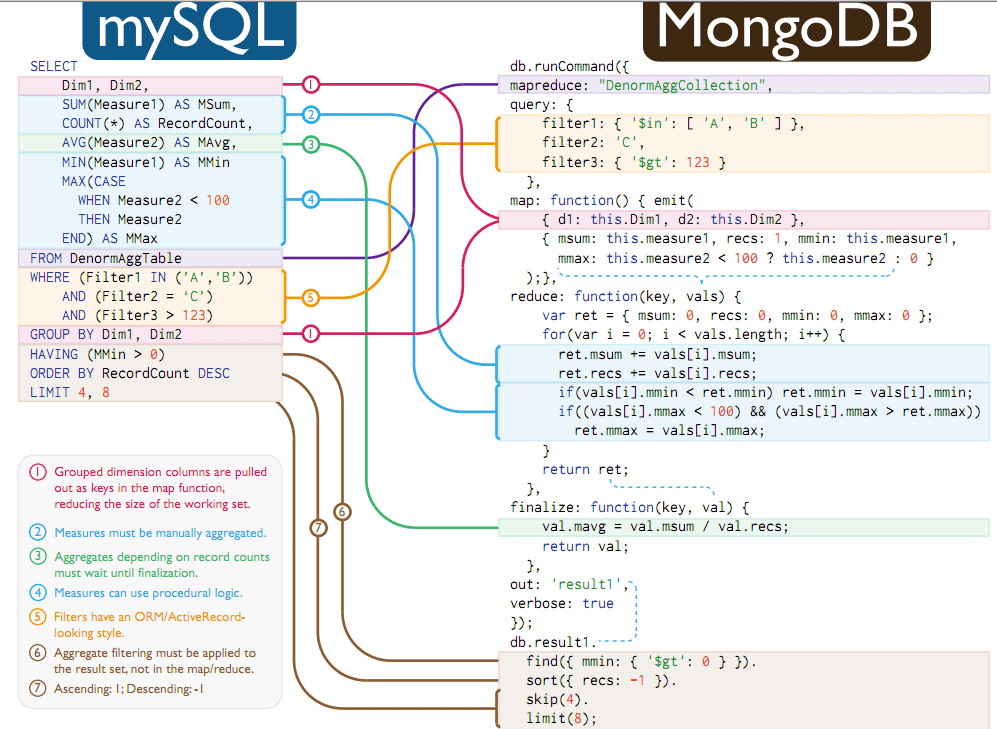
\includegraphics[width=14cm]{5.6.mongodb.png}
   \label{図5.1}
   \caption{MongoDBとMysqlの操作の対応図}
\end{figure}

現在GoでサポートされているmongoDBのもっとも良いドライバはmgo(http://labix.org/mgo)です。このドライバは現在もっともオフィシャルのpkgになりそうなものです。

次にどのようにしてGoからmongoDBを操作するのかご説明します:

\begin{lstlisting}[numbers=none]
package main

import (
    "fmt"
    "gopkg.in/mgo.v2"
    "gopkg.in/mgo.v2/bson"
    "log"
)

type Person struct {
    Name  string
    Phone string
}

func main() {
    session, err := mgo.Dial("server1.example.com,server2.example.com")
    if err != nil {
        panic(err)
    }
    defer session.Close()

    // Optional. Switch the session to a monotonic behavior.
    session.SetMode(mgo.Monotonic, true)

    c := session.DB("test").C("people")
    err = c.Insert(&Person{"Ale", "+55 53 8116 9639"},
        &Person{"Cla", "+55 53 8402 8510"})
    if err != nil {
        log.Fatal(err)
    }

    result := Person{}
    err = c.Find(bson.M{"name": "Ale"}).One(&result)
    if err != nil {
        log.Fatal(err)
    }

    fmt.Println("Phone:", result.Phone)
}
\end{lstlisting}

mgoの操作方法とbeedbの操作方法はほとんど似ていることがわかります。どちらもstructに基づいて操作する方法です。これこそがGo Styleです。


\subsection{まとめ}
この章ではGoがどのようにdatabase/sqlインターフェースを設計するのかご説明しました。その後、サードパーティによるリレーショナルデータベースドライバの使用をご紹介しました。次にbeedbというリレーショナルデータベースに基づくORMライブラリがどのようにしてデータベースに対して簡単な操作を行うかご説明しました。最後にNOSQLのいくつかの知識をご紹介しました。現在GoのNOSQLに対するサポートはなかなかよくできています。Goは21世紀のC言語ですから、21世紀のデータベースに対するサポートも非常によくできています。

この一章の学習を通じて、いろいろなデータベースをどのように操作するか学んできました。Webの中でも重要なデータの保存に関する問題が解決したので、みなさんのdatabase/sqlの設計思想により一歩進んだ理解が深まることを願っています。

\begin{quote}
Go database/sql tutorial(http://go-database-sql.org/)ではよく使われる例と詳細な説明を提供しています。
\end{quote}




\section{sessionとデータの保存}
Web開発ではどのようにしてユーザの閲覧過程のすべてをコントロールするかということは非常に重要です。HTTPプロトコルはステートレスですので、ユーザの毎回のリクエストにはステータスがありません。Web操作の全体の過程の中でどの接続がどのユーザと関係しているのか知る方法がありません。では、どのようにしてこの問題を解決しているのでしょうか?Webでの伝統的な解決方法はcookieとsessionです。cookieによるメカニズムはクライアント側でのメカニズムです。ユーザのデータをクライアントに保存します。sessionメカニズムはサーバ側でのメカニズムです。サーバはハッシュテーブルのような構造でデータを保存します。ホームページの各閲覧者はユニークなIDを与えられます。すなわち、SessionIDです。この保存形式は2つだけです:urlによって渡されるか、クライアントのcookieに保存されるかです。当然、Sessionをデータベースに保存することもできます。よりセキュリティが高まりますが、効率の面ではいくつか後退します。

6.1節ではsessionメカニズムとcookieメカニズムの関係と区別についてご紹介します。6.2ではGo言語がどのようにsessionを実現しているかご説明します。この中では簡単なsessionマネージャを実現します。6.3節ではどのようにしてsessionハイジャックの状態を防ぐかご説明します。どのように効果的にsessionを保護するのか。sessionはそもそもどのようなところに保存してもよいのです。6.3節ではsessionをメモリの中に保存しますが、我々のアプリケーションをもう一歩展開させる場合、アプリケーションのsession共有を実現する必要があります。sessionをデータベースの中(memcachedまたはredis)に保存します。6.4節ではどのようにしてこの機能を実装するかご説明します。


\subsection{sessionとcookie}
sessionとcookieの2つはホームページの閲覧の中で比較的よくみかける概念です。これらはまた区別するのが難しい概念でもあります。しかし認証の必要なサービスやページの統計では相当重要になってきます。まずsessionとcookieがいったいどういうものか理解していくことにしましょう。このような問題を考えます:

どのようにしてアクセスに制限のあるページをスクレイピングすればよいでしょうか?例えば新浪マイクロブログの友達のメインページや個人のマイクロブログのページ等です。

当然ブラウザから手動でユーザ名とパスワードを入力し、ページにアクセスすることができます。いわゆる"スクレイピング"とはプログラムを使って同じような作業を行うことを言います。そのため、"ログイン"の過程で何が発生しているのか理解する必要があります。

ユーザがマイクロブログのログイン画面にきた時、ユーザ名とパスワードを入力した後、"ログイン"をクリックするとブラウザが認証情報をリモートのサーバに送信します。サーバは検証ロジックを実行して、もし検証がパスすれば、ブラウザはログインしたユーザのマイクロブログのトップページにリダイレクトします。ログインが成功した後、サーバはどのように我々がその他の制限のあるページへのアクセスを検証するのでしょうか?HTTPプロトコルはステートレスですので、サーバは我々が前のHTTPリクエストの中で検証をパスした事を知る由もありません。当然、もっとも簡単な解決方法はすべてのリクエストにユーザ名とパスワードを含めることです。これでも構いませんが、サーバの負荷を非常に高めてしまいます。(毎回のリクエストがすべてデータベースでの検証を必要とします。)ユーザのエクスペリエンスも低下します。(すべてのページで再度ユーザ名とパスワードを入力しなければなりません。すべてのページにログインフォームが出てきます。)直接リクエストの中にユーザ名とパスワードを含めるわけにはいかないのでサーバかクライアントに身分を示す情報のようなものを保存するしかありません。cookieとsessionはそのためにあります。

cookieとは、簡単に言えばローカルマシンに保存されたユーザの操作の履歴情報です(当然ログイン情報を含みます)。またユーザが再度このページにアクセスした際ブラウザはHTTPプロトコルを通してローカルのcookieの内容をサーバに送信し、検証を行います。または継続して前の操作を行います。

\begin{figure}[H]
   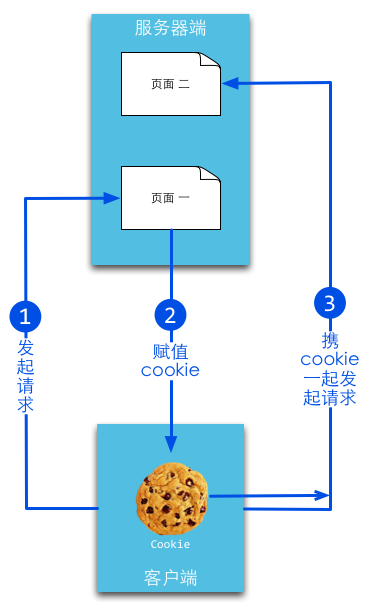
\includegraphics[width=7cm]{6.1.cookie2.png}
   \label{図6.1}
   \caption{cookieの原理図}
\end{figure}

sessionとは、簡単に言えばサーバ上に保存されたユーザの操作の履歴情報です。サーバはsession idを使用してsessionを識別します。session idはサーバが生成します。ランダム性とユニーク性を保証し、ランダムな秘密鍵に相当します。ハンドシェイクやデータ通信中にユーザの本当のパスワードが暴露されるのを防ぎます。しかしこの方法では、依然としてリクエストを送信したクライアントとsessionを対応させる必要があります。そのためcookieメカニズムによってクライアントのID(session id)を取得することで、GETメソッドでidをサーバに送信することができます。

\begin{figure}[H]
   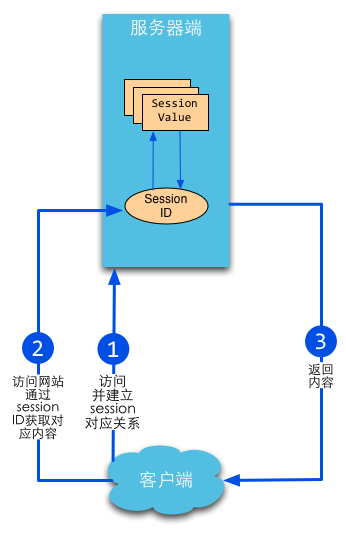
\includegraphics[width=7cm]{6.1.session.png}
   \label{図6.2}
   \caption{sessionの原理図}
\end{figure}




\subsubsection{cookie}
Cookieはブラウザによって維持されます。クライアントに小さな本文情報として保存されます。ユーザのリクエストと画面に沿ってWebサーバとブラウザの間でやりとりされます。ユーザがページにアクセスした際、Webアプリケーションはcookieに含まれる情報を読取ることができます。ブラウザの設定ではcookieのプライバシーデータの選択肢があります。これをオープンするとすでにアクセスしたことのあるページのcookieをたくさん閲覧することができます。下の図をご覧ください:

\begin{figure}[H]
  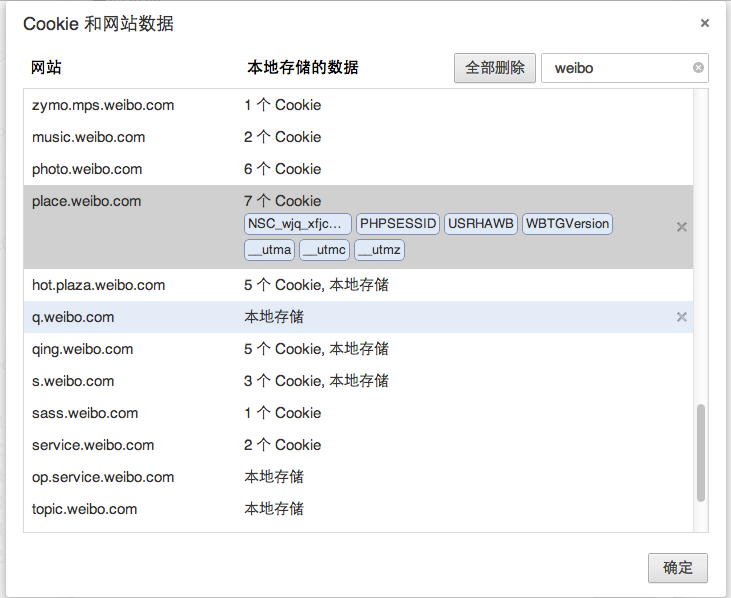
\includegraphics[width=14cm]{6.1.cookie.png}
   \label{図6.3}
   \caption{ブラウザで保存されているcookie情報}
\end{figure}

cookieには有効期限があります。有効期限の違いに従って2つに分けられます:セッションcookieと持続クッキーがあります。

もし有効期限を設定しなければ、このcookieの有効期限は新規に作成されてからブラウザを閉じるまでとなり、cookieは消滅します。このような有効期限は閲覧時のセッションのセッションcookieと呼ばれます。セッションcookieは一般的にハードディスク上には保存されず、メモリに保存されます。

もし有効期限(setMaxAge(606024))が設定されていると、ブラウザはcookieをハードディスクに保存します。ブラウザを閉じて再度開くと、これらのcookieは依然として設定された有効期限まで有効となります。ハードディスク上に保存されたcookieは異なるブラウザのプロセス間で共有することができます。たとえばIEを2つ開き、メモリに保存されたcookieに対し異なるブラウザは異なる処理方法をとります。   



\subsubsection{Goでcookieを設定する}
Go言語ではnet/httpパッケージのSetCookieを通して設定します:


\begin{lstlisting}[numbers=none]
http.SetCookie(w ResponseWriter, cookie *Cookie)
\end{lstlisting}

wは入力する必要のあるresponse、cookieはstructです。cookieオブジェクトがどのようになっているか見てみましょう。

\begin{lstlisting}[numbers=none]
type Cookie struct {
    Name       string
    Value      string
    Path       string
    Domain     string
    Expires    time.Time
    RawExpires string

// MaxAge=0 means no 'Max-Age' attribute specified.
// MaxAge<0 means delete cookie now, equivalently 'Max-Age: 0'
// MaxAge>0 means Max-Age attribute present and given in seconds
    MaxAge   int
    Secure   bool
    HttpOnly bool
    Raw      string
    Unparsed []string // Raw text of unparsed attribute-value pairs
}
\end{lstlisting}

例を一つ見てみましょう。どのようにcookieを設定するかです。

\begin{lstlisting}[numbers=none]
expiration := time.Now()
expiration = expiration.AddDate(1, 0, 0)
cookie := http.Cookie{Name: "username", Value: "astaxie",
                      Expires: expiration}
http.SetCookie(w, &cookie)
\end{lstlisting}



\subsubsection{Goでcookieを読む}
上の例ではどのようにcookieデータを設定するかご説明しました。ここではどのようにcookieを読み取るのか見てみましょう。

\begin{lstlisting}[numbers=none]
cookie, _ := r.Cookie("username")
fmt.Fprint(w, cookie)
\end{lstlisting}

もうひとつのロード方法は

\begin{lstlisting}[numbers=none]
for _, cookie := range r.Cookies() {
    fmt.Fprint(w, cookie.Name)
}
\end{lstlisting}

requestを通してcookieが非常に簡単に取得できるのがおわかりいただけるとおもいます。

\subsubsection{session}
session、中国語ではよく「会話」と翻訳されます。本来は始めから終わりまでの一連のアクション/メッセージを意味します。たとえば電話をかける時は受話器を手にとり電話番号を押して電話を切る間の一連の過程をsessionと呼ぶことができます。しかしsessionという言葉がネットワークプロトコルと関係がある時は、往々にして"接続型通信"または/もしくは"ステートの保持"の2つの意味が含まれています。

sessionはWeb開発環境ではまた新しい意味が含まれます。クライアントサイドとサーバサイドの間でステートを保持するためのソリューションです。しばしばSessionはこのようなソリューションの保存構造も指します。

sessionメカニズムはサーバサイドのメカニズムです。サーバでハッシュテーブルの構造に似たもの(ハッシュテーブルを使う場合もあります)を使用することで情報を保存します。

しかしプログラムがあるクライアントのリクエストにsessionを確立する必要がある場合、サーバはまずこのクライアントのリクエストにsessionIDがあるかを検査します。サーバはsession idを参照し、このsessionを検索し(検索できなかった場合は新規に作成されます。このような状況はサーバがすでにこのユーザに対応するsessionオブジェクトを削除してしまった場合に起こり得ます、しかしユーザは人為的にリクエストのURLの後にSESSIONの引数を追加します。)使用します。もしユーザのリクエストにsession idが含まれなければ、このユーザにsessionを作成し同時にこのsessionと関係するsession idを生成します。このsession idは今回のレスポンスにおいてクライアント側に返され保存されます。

sessionメカニズム自身は特に複雑ではありませんが、その実装と設定の柔軟性は複雑を極めます。これは一回の経験やひとつのブラウザ、サーバのみの経験でもって普遍的に通用するものではありません。

\subsubsection{まとめ}
上述の通り、sessionとcookieの目的は同じです。どちらもhttpプロトコルのステートレスであるという欠点を克服するためにあります。しかしその方法は異なります。sessionはcookieを通じてクライアントにsession idを保存します。またユーザの他のセッション情報はサーバのsessionオブジェクトに保存されます。これとは対照的に、cookieはすべての情報をクライアントに持たせる必要があります。そのためcookieにはある程度潜在的な脅威が存在します。例えばローカルのcookieに保存されたユーザ名とパスワードが解読されたり、cookieが他のホームページに収集されます(例えば:1.appAが主導的にゾーンBのcookieを設定し、ゾーンBにcookieを取得させます;2.XSS、appAでjavascriptを通じてdocument.cookieを取得し、自分のappBに送信します)。

上のいくつかの簡単な紹介でcookieとsessionの基礎的な知識をご紹介しました。これらの間の関係と区別を知り、web開発を行う前に必要な知識をあらかじめよく理解することで、対応に困窮したりbugフィックスを行う際に行き当たりばったりになったりしなくて済みます。以降のいくつかの章ではsessionに関するより細かな知識についてご紹介します。


\subsection{Goはどのようにしてsessionを使用するか}
前の節で、sessionはサーバサイドで実装されるユーザとサーバ間の認証のソリューションのひとつであることをご紹介しました。現在Goの標準パッケージにはsessionのサポートがありません。この節では実際に手を動かしてgoバージョンのsession管理と作成を実現してみます。

\subsubsection{sessionの作成過程}
sessionの基本原理はサーバによって各セッションにおける情報データを保護することです。クライアントサイドはサーバサイドとグローバルでユニークなIDひとつを頼ってこのデータにアクセスし、インタラクティブな目的が達成されます。ユーザがWebアプリケーションにアクセスする際、サーバサイドのプログラムはsession作成の要求に従います。この過程は3つのステップに分けることができます:

\begin{itemize}
  \item グローバルでユニークなIDの生成(sessionid)
  \item データの保存スペースを作成。普通はメモリの中に対応するデータ構造を作成します。しかしこのような状況では、システムは一旦電源が切れると、すべてのセッションデータが消失します。もしeコマースのようなホームページであった場合、これは重大な結果をもたらします。そのため、このような問題を解決するためにセッションデータをファイルの中やデータベースの中に書き込むことができます。当然この場合I/Oオーバーヘッドが増加しますが、ある程度のsessionの永続化は実現できますし、sessionの共有にも有利です。
  \item sessionのグローバルでユニークなIDをクライアントサイドに送信します。
\end{itemize}

上の3つのステップでもっとも重要なのは、どのようにこのsessionのユニークIDを送信するかというステップです。HTTPプロトコルの定義上、データはリクエスト行、ヘッダー部またはBodyの中に含めるしかありません。そのため一般的には2つのよく使われる方法があります:cookieとURLの書き直しです。

\begin{enumerate}
  \item Cookie サーバサイドはSet-cookieヘッダーを設定することでsessionのIDをクライアントサイドに送信することができます。クライアントサイドは以降の各リクエストすべてにこのIDを含めます。またsession情報を含んだcookieの有効期限を0(セッションcookie)、つまりブラウザプロセスの有効期限に設定することもよく行われます。各ブラウザはそれぞれ異なる実装がされていますが、差はそれほど大きくはありません(一般的にはブラウザウィンドウを新規に作成した際に反映されます)。
  \item URLの書き直し いわゆるURLの書き直しとは、ユーザに返されるページの中のすべてのURLの後ろにsessionIDを追加することです。このようにユーザがレスポンスを受け取った後、レスポンスのページの中のどのリンクをクリックしたりフォームを送信しても、すべて自動的にsessionIDが付与されます。これによりセッションの保持を実現します。このような方法はすこし面倒ではありますが、もしクライアントサイドがcookieを禁止している場合、このようなソリューションがまず選ばれます。
\end{enumerate}




\subsubsection{Goでsession管理を実現する}
上のsession作成の課程の解説で、読者はsessionの大体の知識を得られたものと思います。しかし具体的な動的ページ技術においては、またどうやってsessionを実現しているのでしょうか?ここではsessionのライフサイクル(lifecycle)と併せてgo言語バージョンのsession管理を実現します。

\subsubsection{session管理設計}
session管理は以下のいくつかのファクターが関わってきます

\begin{itemize}
  \item グローバルなsessionマネージャ
  \item sessionidがグローバルにユニークであることの保証
  \item 各ユーザをひとつのsessionに関連付ける
  \item sessionの保存(メモリ、ファイル、データベース等に保存できます)
  \item sessionの期限切れ処理
\end{itemize}

以降ではsession管理の全体の設計構想と対応するgoのコード例について解説します:

\subsubsection{Sessionマネージャ}
あるグローバルなsessionマネージャを定義します

\begin{lstlisting}[numbers=none]
type Manager struct {
    cookieName  string     //private cookiename
    lock        sync.Mutex // protects session
    provider    Provider
    maxlifetime int64
}

func NewManager(provideName, cookieName string, maxlifetime int64)
                                                 (*Manager, error) {
    provider, ok := provides[provideName]
    if !ok {
        return nil, fmt.Errorf("session: unknown provide %q
                                  (forgotten import?)", provideName)
    }
    return &Manager{provider: provider, cookieName: cookieName,
                    maxlifetime: maxlifetime}, nil
}
\end{lstlisting}

Goで実現される全体のフローは概ねこのようなものになります。mainパッケージにおいてグローバルなsessionマネージャを作成します。

\begin{lstlisting}[numbers=none]
var globalSessions *session.Manager
//この後init関数で初期化されます。
func init() {
    globalSessions, _ = NewManager("memory","gosessionid",3600)
}
\end{lstlisting}

我々はsessionがサーバサイドに保存されるデータであることを知っています。これはどのような方法で保存されてもかまいません。例えばメモリ、データベースまたはファイルの中に保存します。そのため、Providerインターフェースを抽象化することでトークンsessionマネージャが低レイヤで構造を保存します。

\begin{lstlisting}[numbers=none]
type Provider interface {
    SessionInit(sid string) (Session, error)
    SessionRead(sid string) (Session, error)
    SessionDestroy(sid string) error
    SessionGC(maxLifeTime int64)
}
\end{lstlisting}

\begin{itemize}
  \item SessionInit関数はSessionの初期化を実装します。操作に成功するとこの新しいSession変数を返します。
  \item SessionRead関数はsidが示すSession変数を返します。もし存在しなければ、sidを引数としてSessionInit関数をコールし、真新しいSession変数を新規に作成して、返します。
  \item SessionDestroy関数はsidに対応するSession変数を廃棄するために用いられます。
  \item SessionGCはmaxLifeTimeに従って期限の切れたデータを削除します。
\end{itemize}

ではSessionインターフェースはどのような機能を実装しなければならないのでしょうか?Web開発の経験のある読者であればご存知だとは思いますが、Sessionに対する処理の基本は 値を設定する、値を取得する、値を削除する、現在のsessionIDを取得する の4つの操作となります。ですので我々のSessionインターフェースもこの4つの操作を実装します。

\begin{lstlisting}[numbers=none]
type Session interface {
    Set(key, value interface{}) error //set session value
    Get(key interface{}) interface{}  //get session value
    Delete(key interface{}) error     //delete session value
    SessionID() string                //back current sessionID
}
\end{lstlisting}

\begin{quote}
以上の設計構想はdatabase/sql/driverに由来します。先にインターフェースを定義して、その後実際にsessionを保存する構造が対応するインターフェースを実装し登録すると、対応する機能が使用できるようになります。以下はオンデマンドに登録しsessionの構造を保存するRegister関数の実装です。
\end{quote}


\begin{lstlisting}[numbers=none]
var provides = make(map[string]Provider)

// Register makes a session provide available by the provided name.
// If Register is called twice with the same name or if driver is nil,
// it panics.
func Register(name string, provider Provider) {
    if provider == nil {
        panic("session: Register provide is nil")
    }
    if _, dup := provides[name]; dup {
        panic("session: Register called twice for provide " + name)
    }
    provides[name] = provider
}
\end{lstlisting}



\subsubsection{グローバルでユニークなSession ID}
Session IDはWebアプリケーションにアクセスした各ユーザを識別するために用いられます。その為これはグローバルでユニークであることを保証する必要があります。(GUID)、下のコードはどのようにこの要求を満足させるか示しています。

\begin{lstlisting}[numbers=none]
  func (manager *Manager) sessionId() string {
    b := make([]byte, 32)
    if _, err := io.ReadFull(rand.Reader, b); err != nil {
      return ""
    }
    return base64.URLEncoding.EncodeToString(b)
  }
\end{lstlisting}

\subsubsection{sessionの作成}
各ユーザに対して彼らと結びつくSessionを与えたり取得することで、Session情報に従って操作を検証する必要があります。SessionStartという関数はあるSessionが現在アクセスしているユーザと既に関係しているか検査するために用いられます。もし無ければ新規にこれを作成します。

\begin{lstlisting}[numbers=none]
func (manager *Manager) SessionStart(w http.ResponseWriter,
                                     r *http.Request) (session Session) {
    manager.lock.Lock()
    defer manager.lock.Unlock()
    cookie, err := r.Cookie(manager.cookieName)
    if err != nil || cookie.Value == "" {
        sid := manager.sessionId()
        session, _ = manager.provider.SessionInit(sid)
        cookie := http.Cookie{Name: manager.cookieName,
                              Value: url.QueryEscape(sid),
                              Path: "/", HttpOnly: true,
                              MaxAge: int(manager.maxlifetime)}
        http.SetCookie(w, &cookie)
    } else {
        sid, _ := url.QueryUnescape(cookie.Value)
        session, _ = manager.provider.SessionRead(sid)
    }
    return
}
\end{lstlisting}

前のlogin操作で示したsessionの運用を利用します:

\begin{lstlisting}[numbers=none]
func login(w http.ResponseWriter, r *http.Request) {
    sess := globalSessions.SessionStart(w, r)
    r.ParseForm()
    if r.Method == "GET" {
        t, _ := template.ParseFiles("login.gtpl")
        w.Header().Set("Content-Type", "text/html")
        t.Execute(w, sess.Get("username"))
    } else {
        sess.Set("username", r.Form["username"])
        http.Redirect(w, r, "/", 302)
    }
}
\end{lstlisting}


\subsubsection{値の操作:設定、ロードおよび削除}
SessionStart関数はSessionインターフェースを満足させる変数を返します。ではどのようにこれを利用してsessionデータに対し操作を行うのでしょうか?

上の例のコード\texttt{session.Get("uid")}において基本的なデータのロード操作をお見せしました。ここではより詳しく操作を見ていくことにしましょう:

\begin{lstlisting}[numbers=none]
func count(w http.ResponseWriter, r *http.Request) {
    sess := globalSessions.SessionStart(w, r)
    createtime := sess.Get("createtime")
    if createtime == nil {
        sess.Set("createtime", time.Now().Unix())
    } else if (createtime.(int64) + 360) < (time.Now().Unix()) {
        globalSessions.SessionDestroy(w, r)
        sess = globalSessions.SessionStart(w, r)
    }
    ct := sess.Get("countnum")
    if ct == nil {
        sess.Set("countnum", 1)
    } else {
        sess.Set("countnum", (ct.(int) + 1))
    }
    t, _ := template.ParseFiles("count.gtpl")
    w.Header().Set("Content-Type", "text/html")
    t.Execute(w, sess.Get("countnum"))
}
\end{lstlisting}

上の例には、Sessionの操作とkey/valueデータベースに似た操作である:Set、Get、Deleteといった操作が見受けられます。

Sessionには有効期限の概念がありますので、GC操作を定義しました。アクセス期限が切れるとGCのトリガー条件を満たし、GCを呼び出します。しかし我々が任意のsession操作を行うと、Sessionエンティティに対し更新を行い、最終アクセス時間の修正を行います。このようにGCが行われる際は誤ってまだ使用されているSessionエンティティを削除してしまわないようにします。

\subsubsection{sessionの再設定}
Webアプリケーションにはユーザのログアウト操作があります。ユーザがアプリケーションをログアウトする時、このユーザのsessionデータを破棄する必要があります。上のコードはすでにどのようにsessionの再設定操作を使用するか示しています。ここではこの関数がこの機能を実装します:

\begin{lstlisting}[numbers=none]
//Destroy sessionid
func (manager *Manager) SessionDestroy(w http.ResponseWriter,
                                       r *http.Request){
    cookie, err := r.Cookie(manager.cookieName)
    if err != nil || cookie.Value == "" {
        return
    } else {
        manager.lock.Lock()
        defer manager.lock.Unlock()
        manager.provider.SessionDestroy(cookie.Value)
        expiration := time.Now()
        cookie := http.Cookie{Name: manager.cookieName,
                              Path: "/", HttpOnly: true,
                              Expires: expiration, MaxAge: -1}
        http.SetCookie(w, &cookie)
    }
}
\end{lstlisting}

\subsubsection{sessionの破棄}
ではSessionマネージャがどのように破棄を管理しているのかみてみることにしましょう。Mainが呼び出される際に実行するだけです:

\begin{lstlisting}[numbers=none]
func init() {
    go globalSessions.GC()
}

func (manager *Manager) GC() {
    manager.lock.Lock()
    defer manager.lock.Unlock()
    manager.provider.SessionGC(manager.maxlifetime)
    time.AfterFunc(time.Duration(manager.maxlifetime),
                                 func() { manager.GC() })
}
\end{lstlisting}

GCが十分にtimeパッケージのタイマー機能を利用していることがおわかりいただけるかと思います。時間が\texttt{maxLifeTime}を超えた後GC関数をコールした際、これによって\texttt{maxLiefTime}時間内でsessionが利用できることを保証できます。このような方法はまたオンラインユーザの数といった統計に用いることもできます。

\subsubsection{まとめ}
これまでに、WebアプリケーションにおけるグローバルなSession管理に用いられるSessionManagerを実装してまいりました。Sessionを提供するために用いられるストレージを定義し、Providerのインターフェースを実装しました。次の節では、インターフェースの定義を通してProviderを実装します。ぜひご参考ください。


\subsection{sessionストレージ}
上の節でSessionマネージャの実装原理をご紹介しました。sessionを保存するインターフェースを定義したので、この節ではメモリに基づくsessionストレージインターフェースの実装例をご説明します。その他の保存方法についてはご自身で例を参考に実装してみてください。メモリの実装については下のコード例をご覧ください。

\begin{lstlisting}[numbers=none]
package memory

import (
    "container/list"
    "github.com/astaxie/session"
    "sync"
    "time"
)

var pder = &Provider{list: list.New()}

type SessionStore struct {
    sid          string                      //session idユニークID
    timeAccessed time.Time                   //最終アクセス時間
    value        map[interface{}]interface{} //sessionに保存される値
}

func (st *SessionStore) Set(key, value interface{}) error {
    st.value[key] = value
    pder.SessionUpdate(st.sid)
    return nil
}

func (st *SessionStore) Get(key interface{}) interface{} {
    pder.SessionUpdate(st.sid)
    if v, ok := st.value[key]; ok {
        return v
    } else {
        return nil
    }
    return nil
}

func (st *SessionStore) Delete(key interface{}) error {
    delete(st.value, key)
    pder.SessionUpdate(st.sid)
    return nil
}

func (st *SessionStore) SessionID() string {
    return st.sid
}

type Provider struct {
    lock     sync.Mutex               //ロックに使用します
    sessions map[string]*list.Element //メモリに保存するために使用します
    list     *list.List               //gcを行うために使用します
}

func (pder *Provider) SessionInit(sid string) (session.Session, error) {
    pder.lock.Lock()
    defer pder.lock.Unlock()
    v := make(map[interface{}]interface{}, 0)
    newsess := &SessionStore{sid: sid, timeAccessed: time.Now(), value: v}
    element := pder.list.PushBack(newsess)
    pder.sessions[sid] = element
    return newsess, nil
}

func (pder *Provider) SessionRead(sid string) (session.Session, error) {
    if element, ok := pder.sessions[sid]; ok {
        return element.Value.(*SessionStore), nil
    } else {
        sess, err := pder.SessionInit(sid)
        return sess, err
    }
    return nil, nil
}

func (pder *Provider) SessionDestroy(sid string) error {
    if element, ok := pder.sessions[sid]; ok {
        delete(pder.sessions, sid)
        pder.list.Remove(element)
        return nil
    }
    return nil
}

func (pder *Provider) SessionGC(maxlifetime int64) {
    pder.lock.Lock()
    defer pder.lock.Unlock()

    for {
        element := pder.list.Back()
        if element == nil {
            break
        }
        if (element.Value.(*SessionStore).timeAccessed.Unix() +
                           maxlifetime) < time.Now().Unix() {
            pder.list.Remove(element)
            delete(pder.sessions, element.Value.(*SessionStore).sid)
        } else {
            break
        }
    }
}

func (pder *Provider) SessionUpdate(sid string) error {
    pder.lock.Lock()
    defer pder.lock.Unlock()
    if element, ok := pder.sessions[sid]; ok {
        element.Value.(*SessionStore).timeAccessed = time.Now()
        pder.list.MoveToFront(element)
        return nil
    }
    return nil
}

func init() {
    pder.sessions = make(map[string]*list.Element, 0)
    session.Register("memory", pder)
}
\end{lstlisting}

上のコードはメモリに保存するsessionメカニズムを実現しています。init関数を通じてsessionマネージャに登録されます。このように簡単にコールすることができます。どのようにこのエンジンをコールするのでしょうか?下のコードをご覧ください。


\begin{lstlisting}[numbers=none]
import (
    "github.com/astaxie/session"
    _ "github.com/astaxie/session/providers/memory"
)
\end{lstlisting}

importを行う際、memory関数ではinit関数がすでに実行されています。これによりすでにsessionマネージャへの登録が済んでいますので、使用することができます。下の方法によってsessionマネージャを初期化することができます:

\begin{lstlisting}[numbers=none]
var globalSessions *session.Manager

//この後、init関数で初期化を行います。
func init() {
    globalSessions, _ = session.NewManager("memory", "gosessionid", 3600)
    go globalSessions.GC()
}
\end{lstlisting}




\subsection{sessionハイジャックの予防}
sessionハイジャックは広範囲に存在する比較的重大な脆弱性です。session技術において、クライアントサイドとサーバサイドはsessionのIDによってセッションを維持します。しかしこのIDは簡単にスニッフィングされ、第三者に利用されてしまいます。これは中間者攻撃の一種です。

本章ではセッションハイジャックの実例をお見せします。この実例を通して、読者がよりsessionの本質への理解を深めていただけることを願っています。

\subsubsection{sessionハイジャックの過程}
下のようなcountカウンターを書きます:


\begin{lstlisting}[numbers=none]
func count(w http.ResponseWriter, r *http.Request) {
    sess := globalSessions.SessionStart(w, r)
    ct := sess.Get("countnum")
    if ct == nil {
        sess.Set("countnum", 1)
    } else {
        sess.Set("countnum", (ct.(int) + 1))
    }
    t, _ := template.ParseFiles("count.gtpl")
    w.Header().Set("Content-Type", "text/html")
    t.Execute(w, sess.Get("countnum"))
}
\end{lstlisting}

count.gtplのコードは以下の通り:

\begin{lstlisting}[numbers=none]
Hi. Now count:{{.}}
\end{lstlisting}

ブラウザ上でリロードを行うと以下のような内容が確認できます:

\begin{figure}[H]
  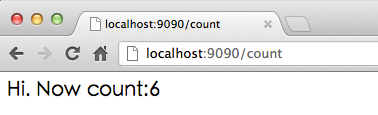
\includegraphics[width=8cm]{6.4.hijack.png}
   \label{図6.4}
   \caption{ブラウザでcount数を表示}
\end{figure}

リロードによって、数字は際限なく増加します。数字が6を示した時ブラウザ(ここではchromeを例にとります)のcookieマネージャを開くと、以下のような情報を見ることができます:

\begin{figure}[H]
  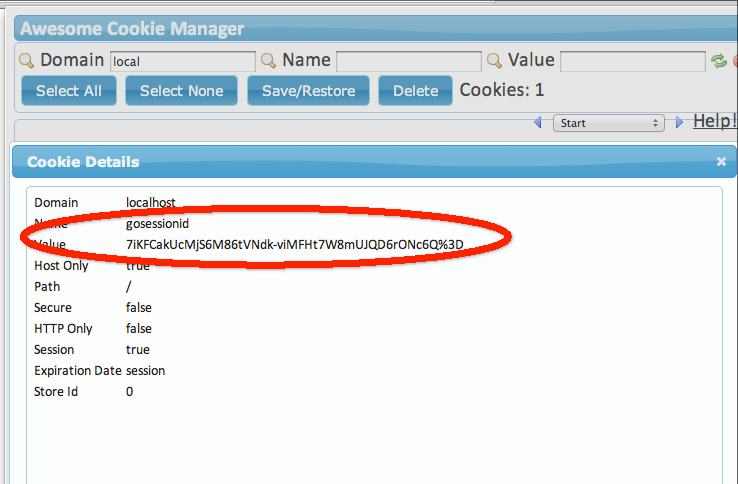
\includegraphics[width=14cm]{6.4.cookie.png}
   \label{図6.5}
   \caption{ブラウザが保存しているcookieを取得}
\end{figure}

次のステップが重要です:別のブラウザ(ここではfirefoxブラウザを開きました)を開き、chromeのアドレスバーのアドレスを新たに開いたブラウザのアドレスバーにコピーします。その後firefoxのcookieエミュレートプラグインを開き、新規にcookieを作成します。上の図のcookieの内容をそのままfirefoxの中に再設定します:

\begin{figure}[H]
  \includegraphics[width=8cm]{6.4.setcookie.png}
   \label{図6.6}
   \caption{cookieをエミュレート}
\end{figure}

エンターキーを押すと、下のような内容が現れます:

\begin{figure}[H]
  \includegraphics[width=8cm]{6.4.hijacksuccess.png}
   \label{図6.7}
   \caption{sessionのハイジャックに成功}
\end{figure}

ブラウザを変えても、sessionIDを取得することができました。この後cookieの保存過程をエミュレートします。この例は一台のコンピュータの上で行ったものです。たとえ二台によって行ったとしても結果は同じです。この時もし交代で2つのブラウザのリンクをクリックした場合、操作しているカウンターが実は同じものであるということに気づくでしょう。驚くことはありません。ここではfirefoxがchromeとgoserver間のセッション維持の鍵を盗みました。すなわち、gosessionidです。これは"セッションハイジャック"の一種です。goserverからすると、httpリクエストからgosessionidを得ました。HTTPプロトコルのステートレスによってgosessionidがchromeから"ハイジャック"されたものなんか知る方法はありません。依然として対応するsessionを探し、関連する計算を実行します。同時にchromeも自分が保持しているセッションがすでに"ハイジャック"されたことを知る方法もありません。


\subsubsection{sessionハイジャックの予防措置}
\paragraph{cookieonlyとtoken}
上のセッションハイジャックの簡単な例で、sessionが他の人にハイジャックされると非常に危険だとわかりました。ハイジャック側はハイジャックされた側を装い多くの非合法な操作を行うことができます。ではどのように効果的にsessionハイジャックを防止するのでしょうか?

ひとつの方法はsessionIDの値にcookieによってのみ設定されるようにすることです。URLの書き直し方法は許さないようにし、同時にcookieのhttponlyをtrueに設定します。このプロパティはクライアントサイドのスクリプトが設定されたcookieにアクセスできるか否かを設定します。まず、これによってこのcookieがXSSによって読み取られ、sessionハイジャックを引き起こすことを防止できます。つぎにcookieの設定がURLの書き直し方法によって容易にsessionIDを取得することができなくなります。

ステップ2は各リクエストの中にtokenを追加することです。前の章で述べたformの重複送信を防止するのに似た機能を実装します。各リクエストの中で隠されたtokenを追加し、毎回このtokenを検証することでユーザのリクエストがユニークであることを保証します。

\begin{lstlisting}[numbers=none]
h := md5.New()
salt:="astaxie%^7&8888"
io.WriteString(h,salt+time.Now().String())
token:=fmt.Sprintf("%x",h.Sum(nil))
if r.Form["token"]!=token{
    //ログイン画面を表示
}
sess.Set("token",token)
\end{lstlisting}

\paragraph{間隔をおいて新しいSIDを生成する}
もう一つの方法は、sessionの他に作成時間を設けることです。一定の時間が過ぎると、このsessionIDは破棄され、再度新しいsessionが生成されます。このようにすることで、ある程度sessionハイジャックの問題を防ぐことができます。

\begin{lstlisting}[numbers=none]
createtime := sess.Get("createtime")
if createtime == nil {
    sess.Set("createtime", time.Now().Unix())
} else if (createtime.(int64) + 60) < (time.Now().Unix()) {
    globalSessions.SessionDestroy(w, r)
    sess = globalSessions.SessionStart(w, r)
}
\end{lstlisting}

sessionが始まると、生成されたsessionIDの時間を記録する一つの値が設定されます。毎回のリクエストが有効期限(ここでは60秒と設定しています)を超えていないか判断し、定期的に新しいIDを生成します。これにより攻撃者は有効なsessionIDを取得する機会を大きく失います。

上の2つの手段を組み合わせると実践においてsessionハイジャックのリスクを取り除くことができます。sessionIDを頻繁に変えると攻撃者に有効なsessionIDを取得する機会を失わせます。sessionIDはcookieの中でやりとりされ、httponlyを設定されるため、URLに基づいた攻撃の可能性はゼロです。同時にXSSによるsessionIDの取得も不可能です。最後にMaxAge=0を設定します。これによりsession cookieがブラウザのログの中に記録されなくなります。



\subsection{まとめ}
この章ではsession/cookieとは何かを、また両者の関係について勉強しました。しかし現在Goのオフィシャルパッケージではsessionがサポートされていません。そのため、sessionマネージャを設計しました。sessionの作成から破棄に至る全体の過程を実装し、Providerのインターフェースを定義することによって、各バックエンドのsessionストレージをサポートできるようにしました。第三節ではメモリストレージによってどのようにsessionの管理を実装するのかご紹介しました。第四節ではsessionハイジャックの過程と、どのようにsessionハイジャックを防止するのかを解説しました。第一章の解説を通して、読者の皆様方にはsessionの実行原理とどのように実現されるか、またどのように安全にsessionを使用するかについて理解いただけるよう望んています。



\section{テキスト処理}
Web開発においてテキスト処理は非常に重要な要素です。往々にして出力または入力する内容に対して処理を行う必要があります。ここでのテキストには文字列、数字、Json、XML等々が含まれます。高性能な一言語としてのGo言語では、これらのテキストの処理はすべてオフィシャルの標準パッケージにサポートされています。また利用中にGo標準ライブラリが巧みに設計されていることに気がつくでしょう。またユーザからすれば非常に簡単にこれらのテキストを処理することができます。本章では4つの節を通してユーザにGo言語のテキスト処理のよい知識をご紹介したいきたいと思います。

XMLは現在多くの標準インターフェースの対話型言語となっています。多くの場合Javaで書かれたwebserverとのやりとりはどれもXML標準にもとづいて行われます。7.1節ではどのようにXMLテキストを処理するかご紹介します。XMLを使用した後あまりに複雑だと気づきます。現在多くのインターネット企業の対外的なAPIでは多くがJSON形式を採用しています。この形式は描写が簡単ですが、意味をよく表現することができます。7.2節ではどのようにこういったJSON形式のデータを処理するかご説明します。正規表現は人に愛され、また恨まれる道具です。このテキスト処理能力は非常に協力です。我々は前のフォームの検証でその強力さをすでに味わっています。7.3節ではどのようにGoの正規表現を利用するのがよいかより詳しく解説していきます。Web開発において非常に重要な部分としてMVCの分離があります。Go言語ではWeb開発中Vにおいて\texttt{template}という専門的にサポートするパッケージがあります。7.4節ではテンプレートをつかってコンテンツをどのように出力するのか詳細に解説していきます。7.5節ではどのようにしてファイルとディレクトリを操作するのか詳しくご紹介します。7.6節のまとめでは文字列に関する操作についてご紹介します。


\subsection{XMLの処理}
XMLはデータと情報のやりとりするための形式として十分普及しています。Webサービスが日々広範囲で応用されてくるにつれ、現在XMLは日常的な開発作業において重要な役割を演じてきました。この節ではGo言語の標準パッケージにあるXML関連のパッケージをご紹介します。

この節ではXMLの規約に関する内容には触れず(もし関連した知識が必要であれば他の文献をあたってください)、どのようにGo言語でXMLファイルをエンコード/デコードするかといった知識についてご紹介します。

あなたが作業員だとして、あなたが管理するすべてのサーバに以下のような内容のxmlの設定ファイルを作成するとします:

\begin{lstlisting}[numbers=none]
<?xml version="1.0" encoding="utf-8"?>
<servers version="1">
    <server>
        <serverName>Shanghai_VPN</serverName>
        <serverIP>127.0.0.1</serverIP>
    </server>
    <server>
        <serverName>Beijing_VPN</serverName>
        <serverIP>127.0.0.2</serverIP>
    </server>
</servers>
\end{lstlisting}

上のXMLドキュメントは2つのサーバの情報を記述しています。サーバ名とサーバのIP情報を含んでいます。以降のGoの例ではこのXML記述に対して操作を行なっていきます。

\subsubsection{XMLの解析}
どのようにして上のXMLファイルを解析するのでしょうか?xmlパッケージの\texttt{Unmarshal}関数を使って目的を達成することができます。

\begin{lstlisting}[numbers=none]
func Unmarshal(data []byte, v interface{}) error
\end{lstlisting}

dataはXMLのデータストリームを受け取ります。vは出力先となる構造体です。定義はinterfaceで、XMLを任意の形式に変換することができます。ここでは主にstructの変換をご紹介します。なぜなら、structとXMLはどちらも似たようなツリー構造の特徴を持っているからです。

コード例は以下の通り:

\begin{lstlisting}[numbers=none]
package main

import (
    "encoding/xml"
    "fmt"
    "io/ioutil"
    "os"
)

type Recurlyservers struct {
    XMLName     xml.Name `xml:"servers"`
    Version     string   `xml:"version,attr"`
    Svs         []server `xml:"server"`
    Description string   `xml:",innerxml"`
}

type server struct {
    XMLName    xml.Name `xml:"server"`
    ServerName string   `xml:"serverName"`
    ServerIP   string   `xml:"serverIP"`
}

func main() {
    file, err := os.Open("servers.xml") // For read access.        
    if err != nil {
        fmt.Printf("error: %v", err)
        return
    }
    defer file.Close()
    data, err := ioutil.ReadAll(file)
    if err != nil {
        fmt.Printf("error: %v", err)
        return
    }
    v := Recurlyservers{}
    err = xml.Unmarshal(data, &v)
    if err != nil {
        fmt.Printf("error: %v", err)
        return
    }

    fmt.Println(v)
}
\end{lstlisting}

XMLは本来ツリー構造のデータ形式なので、対応するgo言語のstruct型を定義することができます。xml.Unmarshalを使ってxmlの中にあるデータを解析し、対応するstructオブジェクトにします。上の例では以下のようなデータを出力します。

\begin{lstlisting}[numbers=none]
{{ servers} 1 [{{ server} Shanghai_VPN 127.0.0.1}
      {{ server} Beijing_VPN 127.0.0.2}]
<server>
    <serverName>Shanghai_VPN</serverName>
    <serverIP>127.0.0.1</serverIP>
</server>
<server>
    <serverName>Beijing_VPN</serverName>
    <serverIP>127.0.0.2</serverIP>
</server>
}
\end{lstlisting}

上の例では、xmlファイルを解析して対応するstructオブジェクトにするには\texttt{xml.Unmarshal}によって行われました。この過程はどのように実現されているのでしょうか?我々のstruct定義の後の方を見てみると\texttt{xml:"serverName"}のような内容があることがわかります。これはstructの特徴の一つです。struct tagと呼ばれています。これはリフレクションを補助するために用いられます。\texttt{Unmarshal}の定義を見てみましょう:

\begin{lstlisting}[numbers=none]
func Unmarshal(data []byte, v interface{}) error
\end{lstlisting}

関数には2つの引数があることがわかります。はじめの引数はXMLデータストリームです。ふたつめは保存される対応した型です。現在struct、sliceおよびstringをサポートしています。XMLパッケージの内部ではリフレクションを採用してデータのリフレクションを行なっています。そのため、vの中のフィールドは必ずエクスポートされなければなりません。\texttt{Unmarshal}が解析する際XML要素とフィールドはどのように対応づけられるのでしょうか?これは優先度のあるロードプロセスです。まずstruct tagを読み込み、もしなければ、対応するフィールド名となります。注意しなければならないのは、tag、フィールド名、XML要素を解析する際大文字と小文字を区別するということです。そのため、フィールドは逐一対応していなければなりません。

Go言語のリフレクションメカニズムはこれらのtag情報を使って将来XMLファイルにあるデータをstructオブジェクトに反映させることができます。リフレクションがどのようにstruct tagを利用するかについてのより詳しい内容はreflectの中の対応するコンテンツをご参照ください。

XMLをstructに解析する際は以下のルールに従います:


\begin{itemize}
  \item もしstructのフィールドがstringまたは[]byte型であり、tagに\texttt{",innerxml"}を含む場合は、Unmarshalはこのフィールドが対応する要素の中に含まれるすべてのオリジナルのxmlをこのフィールドに上乗せします。上の例のDescription定義のように、最後の出力は以下のようになります:
    \begin{lstlisting}[numbers=none]
<server>
    <serverName>Shanghai_VPN</serverName>
    <serverIP>127.0.0.1</serverIP>
</server>
<server>
    <serverName>Beijing_VPN</serverName>
    <serverIP>127.0.0.2</serverIP>
</server>
    \end{lstlisting}
  \item もしstructにXMLNameがあり、かつ型がxml.Nameフィールドであれば、解析する際このelementの名前をこのフィールドに保存します。上の例ではserversにあたります。
  \item もしあるstructフィールドのtagの定義においてXML構造のelementの名前が含まれている場合、解析する際対応するelement値をこのフィールドに代入します。上の例ではservernameとserverip定義にあたります。
  \item もしあるstructフィールドのtag定義の中に\texttt{",attr"}とあれば、解析の際にこの構造に対応するelementとフィールド名のプロパティの値をこのフィールドに代入します。上の例のversion定義にあたります。
  \item もしあるstructフィールドのtag定義の型が\texttt{"a>b>c"}のようであれば、解析の際にxml構造のaの下のbの下のc要素の値をこのフィールドに代入します。
  \item もしあるstructフィールドのtagが\texttt{"-"}を定義していると、このフィールドに対してはいかなるマッチしたxmlデータも解析しません。
  \item もしstructフィールドの後のtagに\texttt{",any"}が定義されていると、もしこの子要素が他のルールを満足していない場合にこのフィールドにマッチします。
  \item もしあるXML要素がひとつまたは複数のコメントを含んでいる場合、これらのコメントはひとつめのtagに含まれる"comments"のフィールドに上乗せされます。このフィールドの型は[]byteやstringである可能性があります。もしこのようなフィールドが存在しなければ、コメントは破棄されます。
\end{itemize}

上でどのようにstructのtagを定義するか詳細に述べました。tagが正しく設定されていさえすれば、XML解析は上の例のように簡単になります。tagとXMLのelementは一つ一つ対応しています。上で示したとおり、sliceによって複数の同じレベルの要素を表現することもできます。

\begin{quote}
注意:正しく解析するために、go言語のxmlパッケージはstructの定義の中ですべてのフィールドがエクスポート可能である必要があります。(つまり、頭文字が大文字であるということです。)
\end{quote}


\subsubsection{XMLの出力}
もし我々が上で示したようなXMLファイルを解析したいのではなく、生成したいとしたら、go言語ではどのように実現すべきでしょうか?xmlパッケージで提供される\texttt{Marshal}と\texttt{MarshalIndent}という2つの関数で我々の需要を満たすことができます。この2つの関数の主な違いは2つ目の関数はプレフィックスを増加したり短縮したりする可能性があるということです。関数の定義は下の通り:

\begin{lstlisting}[numbers=none]
func Marshal(v interface{}) ([]byte, error)
func MarshalIndent(v interface{}, prefix, indent string) ([]byte, error)
\end{lstlisting}

2つの関数のはじめの引数はXMLの構造体が定義する型のデータを生成するために用いられます。どちらも生成したXMLデータストリームを返します。

ここでは上のXMLをどのように出力するのか見てみましょう:

\begin{lstlisting}[numbers=none]
package main

import (
    "encoding/xml"
    "fmt"
    "os"
)

type Servers struct {
    XMLName xml.Name `xml:"servers"`
    Version string   `xml:"version,attr"`
    Svs     []server `xml:"server"`
}

type server struct {
    ServerName string `xml:"serverName"`
    ServerIP   string `xml:"serverIP"`
}

func main() {
    v := &Servers{Version: "1"}
    v.Svs = append(v.Svs, server{"Shanghai_VPN", "127.0.0.1"})
    v.Svs = append(v.Svs, server{"Beijing_VPN", "127.0.0.2"})
    output, err := xml.MarshalIndent(v, "  ", "    ")
    if err != nil {
        fmt.Printf("error: %v\n", err)
    }
    os.Stdout.Write([]byte(xml.Header))

    os.Stdout.Write(output)
}
\end{lstlisting}

上のコードは以下のような情報を出力します:

\begin{lstlisting}[numbers=none]
<?xml version="1.0" encoding="UTF-8"?>
<servers version="1">
<server>
    <serverName>Shanghai_VPN</serverName>
    <serverIP>127.0.0.1</serverIP>
</server>
<server>
    <serverName>Beijing_VPN</serverName>
    <serverIP>127.0.0.2</serverIP>
</server>
</servers>
\end{lstlisting}

我々が以前定義したファイルの形式とまったく同じです。\texttt{os.Stdout.Write([]byte(xml.Header))}というコードが出現したのは、\texttt{xml.MarshalIndent}または\texttt{xml.Marshal}が出力する情報がどちらもXMLヘッダを持たないためです。正しいxmlファイルを生成するために、xmlパッケージであらかじめ定義されているHeader変数を使用しました。

\texttt{Marshal}関数が受け取る引数vはinterface{}型です。つまり任意の型の引数を受け取れることを示しています。ではxmlパッケージはどのようなルールにしたがって対応するXMLファイルを生成しているのでしょうか?

\begin{itemize}
  \item もしvがarrayまたはsliceであれば、各要素を出力します。value</tape>のようなものです。
  \item もしvがポインタであれば、Marshalポインタが指し示す内容となります。もしポインタが空であれば、何も出力しません。
  \item もしvがinterfaceであれば、interfaceが含むデータを処理します。
  \item もしvがその他のデータ型であれば、このデータ型がもつフィールド情報を出力します。
\end{itemize}

また、生成されるXMLファイルの中のelementの名前はどのように決定するのでしょうか?要素名は下の優先度に従ってstructの中より取得されます:

\begin{itemize}
  \item もしvがstructであれば、XMLNameのtagで定義されている名前となります。
  \item 型がxml.Nameの名前であれば、XMLNameのフィールドの値が呼ばれます。
  \item structのフィールドのtagを通して取得されます。
  \item structのフィールド名を通して取得されます。
  \item marshallの型名になります。
\end{itemize}

どのようにしてstructの中のフィールドのtag情報を設定し、最終的なxmlファイルの生成をコントロールするのでしょうか?

\begin{itemize}
  \item XMLNameは出力されません
  \item tagに含まれる\texttt{"-"}のフィールドは出力されません
  \item tagに含まれる\texttt{"name,attr"}では、nameをプロパティ名、フィールド値を値としてこのXML要素を出力します。
  \item tagに含まれる\texttt{",attr"}では、このstructのフィールド名をプロパティ名としてXML要素の属性を出力します。上と同じようにこのnameのデフォルト値がフィールド名となるだけです。
  \item tagに含まれる\texttt{",chardata"}では、xmlのcharacter dataが出力されます。elementではありません。
  \item tagに含まれる\texttt{",innerxml"}では、元の通り出力されます。一般的なエンコーディングプロセスは行われません。
  \item tagに含まれる\texttt{",comment"}では、xmlコメントとして出力されます。一般的なエンコーディングプロセスは行われません。フィールドの値には"--"という文字列を含めることができません。
  \item tagに含まれる\texttt{"omitempty"}では、もしこのフィールドの値が空であればこのフィールドはXMLに出力されません。空の値には以下が含まれます: false、0、nilポインタまたはnilインターフェースまたは長さが0のarray、slice、map、string。
  \item tagに含まれる\texttt{"a>b>c"}では、3つの要素aが含むb、bが含むcが順番に出力されます。例えば以下のコードではこうなります:
    \begin{lstlisting}[numbers=none]
FirstName string   `xml:"name>first"`
LastName  string   `xml:"name>last"`

<name>
<first>Asta</first>
<last>Xie</last>
</name>
    \end{lstlisting}
\end{itemize}

ここではどのようにGo言語のxmlパッケージを使ってXMLファイルをエンコード/デコードするかご紹介しました。大切なのはXMLのすべての操作はすべてstruct tagによって実現されているという点です。より詳しい内容またはtagの定義については対応するオフィシャルドキュメントをご参照ください。




\subsection{JSONの処理}
JSON(Javascript Object Notation)は軽量なデータ記述言語です。文字を基礎とした言語のテキスト形式で、C言語ファミリーに似た習慣を採用しています。JSONとXMLの最も大きな違いはXMLが完全なマークアップ言語であるのに対し、JSONがそうでない点です。JSONはXMLに比べ小さく、早く簡単に解析でき、ブラウザのビルトインの素早い解析のサポートもあり、ネットワークのデータ転送分野により適しています。現在我々が見ることのできる多くのオープンプラットフォームでは基本的にJSONをデータ交換のインターフェースとして採用しています。JSONはWeb開発の中でもこのように重要でありますから、Go言語ではJSONのサポートはどうなっているのでしょうか?Go言語の標準ライブラリはすでに非常に良くJSONをサポートしています。JSONデータに対してとても簡単にエンコード/デコードといった作業を行うことができます。

前の節の操作の例でJSONを使って表示しました。結果は以下の通りです:

\begin{lstlisting}[numbers=none]
{"servers":[{"serverName":"Shanghai_VPN","serverIP":"127.0.0.1"},
    {"serverName":"Beijing_VPN","serverIP":"127.0.0.2"}]}
\end{lstlisting}

この節の残りの内容はこのJSONデータをもとに、go言語のjsonパッケージによるJSONデータのエンコード/デコードをご紹介します。

\subsubsection{JSONの解析}
\paragraph{構造体に解析する}
上のようなJSON文字列があると仮定します。ではどのようにこのJSON文字列を解析するのでしょうか?GoのJSONパッケージには以下のような関数があります

\begin{lstlisting}[numbers=none]
func Unmarshal(data []byte, v interface{}) error
\end{lstlisting}

この関数を使って解析の目的を実現することができます。詳細な解析の例は以下のコードをご覧ください:

\begin{lstlisting}[numbers=none]
package main

import (
    "encoding/json"
    "fmt"
)

type Server struct {
    ServerName string
    ServerIP   string
}

type Serverslice struct {
    Servers []Server
}

func main() {
    var s Serverslice
    str := `{"servers":[{"serverName":"Shanghai_VPN",
                         "serverIP":"127.0.0.1"},
                          {"serverName":"Beijing_VPN",
                           "serverIP":"127.0.0.2"}]}`
    json.Unmarshal([]byte(str), &s)
    fmt.Println(s)
}
\end{lstlisting}



上のコード例の中では、まずjsonデータに対応する構造体を定義します。配列はsliceに、フィールド名はJSONの中のKEYに相当します。解析の際どのようにjsonデータとstructフィールドをマッチさせるのでしょうか?例えばJSONのkeyが\texttt{Foo}であった場合、どのようにして対応するフィールドを探すのでしょうか?

\begin{itemize}
  \item まずtagに含まれる\texttt{Foo}のエクスポート可能なstructフィールド(頭文字が大文字)を探し出します。
  \item 次にフィールド名が\texttt{Foo}のエクスポートフィールドを探し出します。
  \item 最後に\texttt{FOO}または\texttt{FoO}のような頭文字を除いたその他の大文字小文字を区別しないエクスポートフィールドを探し出します。
\end{itemize}

聡明なあなたであればお気づきかもしれません:代入されうるフィールドはエクスポート可能なフィールドである必要があります。(すなわち、頭文字が大文字であるということです。)同時にJSONを解析する際探しだせるフィールドを解析するのみで、探せないフィールドについては無視されます。これのメリットは:とても大きなJSONデータ構造を受け取ってしまいその中のいち部分のデータだけを取得したいような場合です。あなたは必要なデータに対応するフィールド名の大文字だけで簡単にこの問題を解決することができます。

\paragraph{interfaceに解析する}
上のような解析方法は解析されるJSONデータの構造を事前に知っている場合に採用されるソリューションです。もし解析されるデータの形式が事前に分からなかった場合はどのように解析すればよいでしょうか?

我々はinterface{}に任意のデータ型のオブジェクトを保存できることを知っています。このようなデータ構造は未知の構造のjsonデータの解析結果を保存するのにぴったりです。JSONパッケージではmap[string]interface{}と[]interface{}構造を採用して任意のJSONオブジェクトと配列を保存します。Goの型とJSONの型の対応関係は以下の通りです:

\begin{itemize}
  \item bool は JSON booleans を表します,
  \item float64 は JSON numbers を表します,
  \item string は JSON string を表します,
  \item nil は JSON null を表します,
\end{itemize}

現在以下のようなJSONデータがあるものと仮定します

\begin{lstlisting}[numbers=none]
b := []byte(`{"Name":"Wednesday","Age":6,"Parents":["Gomez","Morticia"]}`)
\end{lstlisting}

この構造を知らない段階では、これをinterface{}の中に解析します。

\begin{lstlisting}[numbers=none]
var f interface{}
err := json.Unmarshal(b, &f)
\end{lstlisting}

この時fの中にはmap型が保存されます。これらのkeyはstringで、値は空のinterface{]の中に保存されます。

\begin{lstlisting}[numbers=none]
f = map[string]interface{}{
    "Name": "Wednesday",
    "Age":  6,
    "Parents": []interface{}{
        "Gomez",
        "Morticia",
    },
}
\end{lstlisting}

ではどのようにしてこれらのデータにアクセスするのでしょうか?アサーションによる方法です:

\begin{lstlisting}[numbers=none]
m := f.(map[string]interface{})
\end{lstlisting}

アサーションを通して以下のような方法で中のデータにアクセスすることができます。

\begin{lstlisting}[numbers=none]
for k, v := range m {
    switch vv := v.(type) {
    case string:
        fmt.Println(k, "is string", vv)
    case int:
        fmt.Println(k, "is int", vv)
    case float64:
        fmt.Println(k,"is float64",vv)
    case []interface{}:
        fmt.Println(k, "is an array:")
        for i, u := range vv {
            fmt.Println(i, u)
        }
    default:
        fmt.Println(k, "is of a type I don't know how to handle")
    }
}
\end{lstlisting}

上の例では、interface{}とtype assertの組み合わせによって未知の構造のJSONデータを解析することができました。

これはオフィシャルが提供するソリューションです。実は多くの場合、型のアサーションは操作からしてあまり便利ではありません。現在bitly社では\texttt{simplejson}と呼ばれるパッケージがオープンに開発されています。未知の構造体のJSONを処理する場合にとても便利です。詳細な例は以下の通り:

\begin{lstlisting}[numbers=none]
js, err := NewJson([]byte(`{
    "test": {
        "array": [1, "2", 3],
        "int": 10,
        "float": 5.150,
        "bignum": 9223372036854775807,
        "string": "simplejson",
        "bool": true
    }
}`))

arr, _ := js.Get("test").Get("array").Array()
i, _ := js.Get("test").Get("int").Int()
ms := js.Get("test").Get("string").MustString()
\end{lstlisting}

このようにこのライブラリを使用してJSONを操作するのはオフィシャルパッケージに比べてとても簡単です。詳細は以下のアドレスをご参照ください:https://github.com/bitly/go-simplejson

\subsubsection{JSONを生成する}
多くのアプリケーションを開発する際、最後はJSONデータ文字列を出力する必要があります。ではどのようにして処理するのでしょうか?JSONパッケージでは\texttt{Marshal}関数を通して処理します。関数の定義は以下の通り:


\begin{lstlisting}[numbers=none]
func Marshal(v interface{}) ([]byte, error)
\end{lstlisting}

上のサーバのリスト情報を出力する必要があるものと仮定します。どのように処理すべきでしょうか?下の例をご覧ください:

\begin{lstlisting}[numbers=none]
package main

import (
    "encoding/json"
    "fmt"
)

type Server struct {
    ServerName string
    ServerIP   string
}

type Serverslice struct {
    Servers []Server
}

func main() {
    var s Serverslice
    s.Servers = append(s.Servers, Server{ServerName: "Shanghai_VPN",
                                         ServerIP: "127.0.0.1"})
    s.Servers = append(s.Servers, Server{ServerName: "Beijing_VPN",
                                         ServerIP: "127.0.0.2"})
    b, err := json.Marshal(s)
    if err != nil {
        fmt.Println("json err:", err)
    }
    fmt.Println(string(b))
}
\end{lstlisting}

下のような内容が出力されます:

\begin{lstlisting}[numbers=none]
{"Servers":[{"ServerName":"Shanghai_VPN","ServerIP":"127.0.0.1"},
    {"ServerName":"Beijing_VPN","ServerIP":"127.0.0.2"}]}
\end{lstlisting}

上で出力されたフィールド名の頭文字はどれも大文字です。もし頭文字に小文字を使いたい場合はどうすればよいでしょうか?構造体のフィールド名の頭文字を小文字にすべきでしょうか?JSONで出力する際に注意が必要なのは、エクスポートされたフィールドのみが出力されるということです。もしフィールド名を修正してしまうと、何も出力されなくなってしまいます。ですので必ずstruct tagによって定義した上で実装する必要があります:

\begin{lstlisting}[numbers=none]
type Server struct {
    ServerName string `json:"serverName"`
    ServerIP   string `json:"serverIP"`
}

type Serverslice struct {
    Servers []Server `json:"servers"`
}
\end{lstlisting}

上の構造体の定義を修正することで、出力されるJSON文字列と我々が最初に定義したJSON文字列は一致します。

JSONの出力に対して、struct tagを定義する場合注意すべきいくつかのことは:

\begin{itemize}
  \item フィールドのtagが\texttt{"-"}であった場合、このフィールドはJSONに出力されません。
  \item tagにカスタム定義の名前が含まれる場合、このカスタム定義された名前はJSONのフィールド名に出現します。例えば上の例のserverNameに当たります。
  \item tagに\texttt{"omitempty"}オプションが含まれる場合、このフィールドの値が空であればJSON文字列の中には出力されません。
  \item もしフィールドの型がbool, string, int, int65等で、tagに\texttt{",string"}オプションが含まれる場合、このフィールドがJSONに出力される際はこのフィールドに対応した値が変換されてJSON文字列となります。
\end{itemize}

例をあげてご説明しましょう:

\begin{lstlisting}[numbers=none]
type Server struct {
    // ID はJSONの中にエクスポートされません。
    ID int `json:"-"`

    // ServerName2 の値は二次JSONエンコーディングが行われます。
    ServerName  string `json:"serverName"`
    ServerName2 string `json:"serverName2,string"`

    // もし ServerIP が空であれば、JSON文字列の中には出力されません。
    ServerIP   string `json:"serverIP,omitempty"`
}

s := Server {
    ID:         3,
    ServerName:  `Go "1.0" `,
    ServerName2: `Go "1.0" `,
    ServerIP:   ``,
}
b, _ := json.Marshal(s)
os.Stdout.Write(b)
\end{lstlisting}

以下のような内容が出力されます:

\begin{lstlisting}[numbers=none]
{"serverName":"Go \"1.0\" ","serverName2":"\"Go \\\"1.0\\\" \""}
\end{lstlisting}

Marshal関数は変換に成功した時のみデータを返します。変換の過程で注意しなければならないのは:

\begin{itemize}
  \item JSONオブジェクトはstringのみをkeyとしてサポートします。そのためmapをエンコードしたい場合は必ずmap[string]Tのような型となります。(TはGo言語の中の任意の型です。)
  \item Channel, complexとfunctionはJSONにはエンコードされません。
  \item ネストしたデータはエンコードされません。さもないとJSONのエンコードは永久ループに入ってしまいます。
  \item ポインタがエンコードされる際はポインタが指定している内容が出力されます。空のポインタはnullを出力します。
\end{itemize}

この節ではどのようにGo言語のjson標準パッケージを使ってJSONデータをエンコードするかご紹介しました。同時にどのようにサードパーティパッケージである\texttt{go-simplejson}を使っていくつかの状況で簡単な操作をご紹介しました。これらを学び運用に慣れることは以降にご紹介するWeb開発においてとても重要になります。





\subsection{正規表現の処理}
正規表現はパターンマッチとテキスト操作の複雑で強力なツールです。正規表現は純粋なテキストマッチングに比べ効率は劣りますが、より柔軟性に富みます。この文法規則に従い作り出されるパターンはオリジナルのテキストからあなたが必要とするほとんどすべての文字列の組み合わせをフィルターすることができます。もしWeb開発の中でなにかしらのテキストデータソースからデータを取り出す必要があれば、この文法規則にしたがって正確なパターン文字列を作ることで意味のあるテキスト情報をデータソースから取り出すことができます。

Go言語は\texttt{regexp}標準パッケージを使うことでオフィシャルに正規表現をサポートしています。もしあなたが他のプログラミング言語において提供されている正規表現と同等の機能を使ったことがあるのであれば、Go言語バージョンでもそれほど門外漢というわけではないはずです。しかしこれらの間でも少しばかりの違いがあります。なぜならGoが実装しているのはRE2スタンダードで、\textbackslash Cを除いて詳細な文法の説明は以下をご参照ください:http://code.google.com/p/re2/wiki/Syntax

文字列処理はそもそも\texttt{strings}パッケージを使うことで検索(Contains、Index)、置換(Replace)と懐石(Split、Join)といった操作を行うことができました。しかしこれらはどれも簡単な文字列操作にすぎません。これらの検索はどれも大文字と小文字を区別しますし、固定された文字列です。もし可変のこういったマッチングを行う必要があれば、実現する方法がありません。当然もし\texttt{strings}パッケージがあなたの問題を解決できるのであれば、できるかぎりこれを使って解決すべきです。なぜならこれらは簡単で、性能と可読性も正規表現に比べてよいからです。

前のフォームの検証の節ですでに正規表現に触れたことを覚えていらっしゃるかもしれません。その時はこれを使って入力された情報が何らかの予め設定された条件を満足しているか検証するのに使いました。使用に際して注意すべきことは:いかなる文字列もすべてUTF-8でエンコードされているということです。以降ではより深くGo言語の\texttt{regexp}パッケージに関連する知識を学んでいきましょう。

\subsubsection{正規表現を使ってマッチングするか判断する}
\texttt{regexp}パッケージでは3つの関数を使ってマッチングを判断します。もしマッチングすればtrueを返し、さもなければfalseを返します。

\begin{lstlisting}[numbers=none]
func Match(pattern string, b []byte) (matched bool, error error)
func MatchReader(pattern string, r io.RuneReader) (matched bool, error error)
func MatchString(pattern string, s string) (matched bool, error error)
\end{lstlisting}

上の3つの関数は同じ機能を実現しています。つまり、\texttt{pattern}が入力ソースにマッチするかを判断しています。マッチングしたらtrueを返し、もし正規表現の解析でエラーが出たらerrorを返します。3つの関数の入力ソースはそれぞれbyte slice、RuneReaderとstringです。

入力がIPアドレスであるかどうか検証したい場合は、どのように判断すべきでしょうか?以下をご覧ください

\begin{lstlisting}[numbers=none]
func IsIP(ip string) (b bool) {
    if m, _ := regexp.MatchString("^[0-9]{1,3}\\.[0-9]{1,3}\\.
                                  [0-9]{1,3}\\.[0-9]{1,3}$", ip); !m {
        return false
    }
    return true
}
\end{lstlisting}

ご覧のとおり、\texttt{regexp}のpatternと我々が通常使用している正規表現は全く一緒です。もう一つ例を見てみましょう:ユーザが文字列を入力し、この入力が正しいかどうか知りたいものとします:



\begin{lstlisting}[numbers=none]
func main() {
    if len(os.Args) == 1 {
        fmt.Println("Usage: regexp [string]")
        os.Exit(1)
    } else if m, _ := regexp.MatchString("^[0-9]+$", os.Args[1]); m {
        fmt.Println("数字です。")
    } else {
        fmt.Println("数字ではありません。")
    }
}
\end{lstlisting}

上の2つの例では、Match(Reader$|$String)を使って文字列が我々の要求に合致しているか判断しています。これらは非常に便利です。


\subsubsection{正規表現を使って内容を取得する}
Matchパターンは文字列の判断に対してのみ使うことができ、文字列の一部分を切り取ったり、文字列にフィルターをかけたり、合致する条件の文字列を取り出したりすることはできません。これらの需要を満足したければ、正規表現の複雑なパターンを使用する必要があります。

我々はよく一種のスクレイピングプログラムが必要となります。下ではスクレイピングを例にどのように正規表現を使って取得したデータに対しフィルタリングまたは切り取りを行うかご説明します:

\begin{lstlisting}[numbers=none]
package main

import (
    "fmt"
    "io/ioutil"
    "net/http"
    "regexp"
    "strings"
)

func main() {
    resp, err := http.Get("http://www.baidu.com")
    if err != nil {
        fmt.Println("http get error.")
    }
    defer resp.Body.Close()
    body, err := ioutil.ReadAll(resp.Body)
    if err != nil {
        fmt.Println("http read error")
        return
    }

    src := string(body)

    //HTMLタグを全て小文字に変換します
    re, _ := regexp.Compile("\\<[\\S\\s]+?\\>")
    src = re.ReplaceAllStringFunc(src, strings.ToLower)

    //<style>タグを除去します
    re, _ = regexp.Compile("\\<style[\\S\\s]+?\\</style\\>")
    src = re.ReplaceAllString(src, "")

    //<script>タグを除去
    re, _ = regexp.Compile("\\<script[\\S\\s]+?\\</script\\>")
    src = re.ReplaceAllString(src, "")

    //<>内の全てのHTMLコードを削除し、改行文字に置き換えます
    re, _ = regexp.Compile("\\<[\\S\\s]+?\\>")
    src = re.ReplaceAllString(src, "\n")

    //連続した改行を除去します
    re, _ = regexp.Compile("\\s{2,}")
    src = re.ReplaceAllString(src, "\n")

    fmt.Println(strings.TrimSpace(src))
}
\end{lstlisting}

この例からわかるように、複雑な正規表現を使用する場合はまずCompileを行います。これは正規表現が正しいかどうかを解析し、もし正しければRegexpを返します。返されたRegexpは任意の文字列で必要な操作を実行することができるようになります。

正規表現の解析は以下のいくつかの方法があります:

\begin{lstlisting}[numbers=none]
func Compile(expr string) (*Regexp, error)
func CompilePOSIX(expr string) (*Regexp, error)
func MustCompile(str string) *Regexp
func MustCompilePOSIX(str string) *Regexp
\end{lstlisting}

CompilePOSIXとCompileの違いはPOSIXにはかならずPOSIX文法を使う必要があるということです。これは最長一致方式を使って検索を行い、Compileではただ最長一致方式が採用されます。(例えば[a-z]\{2,4\}のような正規表現を"aa09aaa88aaaa"というようなテキストに適用する際、CompilePOSIXはaaaaを返します。またCompileが返す正規表現はaaとなります)、前にMustとつく関数は正規表現の文法を解析する際もしパターンが正確な文法でなければ直接panicとならず、Mustのつかないものはただエラーを返します。

どのようにRegexpを作成するか理解したところで、このstructがどのような方法によって我々の文字列操作を提供しているのかもう一度見てみることにしましょう。まず下の検索を行うための関数を見てみます:

\begin{lstlisting}[numbers=none]
func (re *Regexp) Find(b []byte) []byte
func (re *Regexp) FindAll(b []byte, n int) [][]byte
func (re *Regexp) FindAllIndex(b []byte, n int) [][]int
func (re *Regexp) FindAllString(s string, n int) []string
func (re *Regexp) FindAllStringIndex(s string, n int) [][]int
func (re *Regexp) FindAllStringSubmatch(s string, n int) [][]string
func (re *Regexp) FindAllStringSubmatchIndex(s string, n int) [][]int
func (re *Regexp) FindAllSubmatch(b []byte, n int) [][][]byte
func (re *Regexp) FindAllSubmatchIndex(b []byte, n int) [][]int
func (re *Regexp) FindIndex(b []byte) (loc []int)
func (re *Regexp) FindReaderIndex(r io.RuneReader) (loc []int)
func (re *Regexp) FindReaderSubmatchIndex(r io.RuneReader) []int
func (re *Regexp) FindString(s string) string
func (re *Regexp) FindStringIndex(s string) (loc []int)
func (re *Regexp) FindStringSubmatch(s string) []string
func (re *Regexp) FindStringSubmatchIndex(s string) []int
func (re *Regexp) FindSubmatch(b []byte) [][]byte
func (re *Regexp) FindSubmatchIndex(b []byte) []int
\end{lstlisting}

上の18個の関数は入力ソース(byte slice、stringおよびio.RuneReader)の違いに従って下のいくつかのように簡素化することができます。その他はただ入力ソースが異なるだけで、そのほかの機能は基本的に同じです:

\begin{lstlisting}[numbers=none]
func (re *Regexp) Find(b []byte) []byte
func (re *Regexp) FindAll(b []byte, n int) [][]byte
func (re *Regexp) FindAllIndex(b []byte, n int) [][]int
func (re *Regexp) FindAllSubmatch(b []byte, n int) [][][]byte
func (re *Regexp) FindAllSubmatchIndex(b []byte, n int) [][]int
func (re *Regexp) FindIndex(b []byte) (loc []int)
func (re *Regexp) FindSubmatch(b []byte) [][]byte
func (re *Regexp) FindSubmatchIndex(b []byte) []int
\end{lstlisting}

これらの関数の使用に対して以下の例を見てみましょう

\begin{lstlisting}[numbers=none]
package main

import (
    "fmt"
    "regexp"
)

func main() {
    a := "I am learning Go language"

    re, _ := regexp.Compile("[a-z]{2,4}")

    //正規表現にマッチする最初のものを探し出す
    one := re.Find([]byte(a))
    fmt.Println("Find:", string(one))

    //正規表現にマッチするすべてのsliceを探し出す。
    //nが0よりも小さかった場合はすべてのマッチする
    //文字列を返します。さもなければ指定した長さが返ります。
    all := re.FindAll([]byte(a), -1)
    fmt.Println("FindAll", all)

    //条件にマッチするindexの位置を探し出す。開始位置と終了位置。
    index := re.FindIndex([]byte(a))
    fmt.Println("FindIndex", index)

    //条件にマッチするすべてのindexの位置を探し出す、nは同上
    allindex := re.FindAllIndex([]byte(a), -1)
    fmt.Println("FindAllIndex", allindex)

    re2, _ := regexp.Compile("am(.*)lang(.*)")

    //Submatchを探し出し、配列を返します。はじめの要素は
    //マッチしたすべての要素です。2つ目の要素ははじめの()
    //の中で、3つ目は2つ目の()の中です。
    //以下の出力でははじめの要素は"am learning Go language"です。
    //2つ目の要素は" learning Go "です。空白を含んで出力すること
    //に注意してください。
    //3つ目の要素は"uage"です。
    submatch := re2.FindSubmatch([]byte(a))
    fmt.Println("FindSubmatch", submatch)
    for _, v := range submatch {
        fmt.Println(string(v))
    }

    //定義と上のFindIndexは同じです。
    submatchindex := re2.FindSubmatchIndex([]byte(a))
    fmt.Println(submatchindex)

    //FindAllSubmatchは条件にマッチするすべてのサブマッチを探し出します。
    submatchall := re2.FindAllSubmatch([]byte(a), -1)
    fmt.Println(submatchall)

    //FindAllSubmatchIndexはすべてのサブマッチのindexを探し出します。
    submatchallindex := re2.FindAllSubmatchIndex([]byte(a), -1)
    fmt.Println(submatchallindex)
}
\end{lstlisting}

ここまででマッチ関数をご紹介しました。Regexpも3つの関数を定義しています。これらは同盟の外部関数と機能はまったく一緒です。じつは、外部関数はこのRegexpの3つの関数をコールすることで実現しています。

\begin{lstlisting}[numbers=none]
func (re *Regexp) Match(b []byte) bool
func (re *Regexp) MatchReader(r io.RuneReader) bool
func (re *Regexp) MatchString(s string) bool
\end{lstlisting}

次に置換関数はどのように操作するか理解していきましょう。

\begin{lstlisting}[numbers=none]
func (re *Regexp) ReplaceAll(src, repl []byte) []byte
func (re *Regexp) ReplaceAllFunc
               (src []byte, repl func([]byte) []byte) []byte
func (re *Regexp) ReplaceAllLiteral(src, repl []byte) []byte
func (re *Regexp) ReplaceAllLiteralString(src, repl string) string
func (re *Regexp) ReplaceAllString(src, repl string) string
func (re *Regexp) ReplaceAllStringFunc
              (src string, repl func(string) string) string
\end{lstlisting}


これらの置換関数は上のスクレイピングの例に詳細な応用例があります。

次にExpandの解説を見てみましょう:

\begin{lstlisting}[numbers=none]
func (re *Regexp) Expand(dst []byte, template []byte,
                         src []byte, match []int) []byte
func (re *Regexp) ExpandString(dst []byte, template string,
                         src string, match []int) []byte
\end{lstlisting}

Expandは一体何に使われるのでしょうか?下の例をご覧ください:

\begin{lstlisting}[numbers=none]
func main() {
    src := []byte(`
        call hello alice
        hello bob
        call hello eve
    `)
    pat := regexp.MustCompile(`(?m)(call)\s+(?P<cmd>\w+)\s+(?P<arg>.+)\s*$`)
    res := []byte{}
    for _, s := range pat.FindAllSubmatchIndex(src, -1) {
        res = pat.Expand(res, []byte("$cmd('$arg')\n"), src, s)
    }
    fmt.Println(string(res))
}
\end{lstlisting}

これまでに既にGo言語の\texttt{regexp}パッケージの全てをご紹介しました。これに対する主な関数の紹介と例を通して、みなさんはGo言語の正規表現パッケージを使って基本的な正規表現の操作が可能になったことと信じております。



\subsection{テンプレートの処理}
\subsubsection{テンプレートとは何か}
おそらくあなたはMVCのデザインパターンについて聞いたことがあると思います。Modelはデータを処理を、Viewは表示結果を、Controllerはユーザのリクエストの制御を行います。Viewレイヤーの処理では、多くの動的な言語ではどれも静的なHTMLの中に動的言語が生成したデータを挿入します。例えばJSPでは\texttt{<\%=....=\%>}を挿入することで、PHPでは\texttt{<?php.....?>}を挿入することで実現します。

下の図でテンプレートのメカニズムについてご紹介します

\begin{figure}[H]
  \includegraphics[width=14cm]{7.4.template.png}
   \label{図7.1}
   \caption{テンプレートのメカニズム図}
\end{figure}


Webアプリケーションがクライアントに返すフィードバックの情報の中の大部分の内容は静的で不変です。また少ない部分でユーザのリクエストによって動的に生成されるものがあります。例えばユーザのアクセスログリストを表示したい場合、ユーザ間ではログデータが異なるのみで、リストのスタイルは固定です。この時テンプレートを用いることで多くの静的なコードを使いまわすことができます。

\subsubsection{Goのテンプレートの使用}
Go言語では、\texttt{template}パッケージを使用してテンプレートの処理を行います。\texttt{Parse}、\texttt{ParseFile}、\texttt{Execute}といった方法を使ってファイルや文字列からテンプレートをロードします。その後植えの図で示したテンプレートのmerge操作のようなものを実行します。下の例をご覧ください:

\begin{lstlisting}[numbers=none]
func handler(w http.ResponseWriter, r *http.Request) {
    t := template.New("some template") //テンプレートを新規に作成する。
    t, _ = t.ParseFiles("tmpl/welcome.html", nil)  //テンプレートファイルを解析
    user := GetUser() //現在のユーザの情報を取得する。
    t.Execute(w, user)  //テンプレートのmerger操作を実行する。
}
\end{lstlisting}

上の例で、Go言語のテンプレート操作は非常に簡単で便利だとおわかりいただけるかと思います。その他の言語のテンプレート処理に似ていて、まずデータを取得した後データを適用します。

デモとテストコードの簡便のため、以降の例では以下の形式のコードを採用します。

\begin{itemize}
  \item ParseFilesの代わりにParseを使用します。Parseは直接文字列をテストでき、外部のファイルを必要としないためです。
  \item handlerを使ってデモコードを書くことはせず、それぞれひとつのmainをテストします。便利なテストです。
  \item \texttt{http.ResponseWriter}の代わりに\texttt{os.Stdout}を使用します。\texttt{os.Stdout}は\texttt{io.Writer}インターフェースを実装しているからです。
\end{itemize}


\subsubsection{どのようにしてテンプレートの中にデータを挿入するのか?}
上においてどのように解析とテンプレートの適用するかデモを行いました。以降ではさらに詳しくどのようにデータを適用していくのか理解していきましょう。テンプレートはすべてGoのオブジェクト上で適用されます。Goオブジェクトのフィールドはどのようにしてテンプレートの中に挿入されるのでしょうか?

\paragraph{フィールドの操作}
Go言語のテンプレートは\texttt{\{\{\}\}}を通して適用時に置換する必要のあるフィールドを含めます。\texttt{\{\{.\}\}}は現在のオブジェクトを示しています。これはJavaやC++の中のthisに似たものです。もし現在のオブジェクトのフィールドにアクセスしたい場合は\texttt{\{\{.FieldName\}\}}というようにします。ただし注意してください:このフィールドは必ずエクスポートされたものとなります(頭文字が大文字になります)、さもなければ適用時にエラーを発生させます。下の例をご覧ください:

\begin{lstlisting}[numbers=none]
package main

import (
    "html/template"
    "os"
)

type Person struct {
    UserName string
}

func main() {
    t := template.New("fieldname example")
    t, _ = t.Parse("hello {{.UserName}}!")
    p := Person{UserName: "Astaxie"}
    t.Execute(os.Stdout, p)
}
\end{lstlisting}

上のコードでは正しく\texttt{hello Astaxie}と出力されます。しかしもしコードに修正を加え、テンプレートにエクスポートされていないフィールドを含むと、エラーを発生させます。

\begin{lstlisting}[numbers=none]
type Person struct {
    UserName string
    email    string  //エクスポートされていないフィールド、頭文字が小文字です。
}

t, _ = t.Parse("hello {{.UserName}}! {{.email}}")
\end{lstlisting}

上のコードはエラーを発生させます。なぜならエクスポートされていないフィールドをコールしたためです。しかしもし存在しないフィールドをコールした場合はエラーを発生させず、空文字列を出力します。

テンプレートで\texttt{\{\{.\}\}}を出力すると、一般的には文字列オブジェクトに対して適用されます。デフォルトでfmtパッケージがコールされ文字列の内容が出力されます。



\paragraph{ネストしたフィールドの内容の出力}
上の例でどのようにひとつのオブジェクトのフィールドを出力するか示しました。もしフィールドの中にまたオブジェクトがある場合は、どのようにループしてこれらの内容を出力するのでしょうか?ここでは\texttt{\{\{with ...\}\}...\{\{end\}\}}と\texttt{\{\{range ...\}\}\{\{end\}\}}によってデータを出力することができます。

\begin{itemize}
  \item \{\{range\}\} はGo言語の中のrangeに似ています。ループしてデータを操作します
  \item \{\{with\}\}操作は現在のオブジェクトの値を指します。コンテキストの概念に似ています。
\end{itemize}

詳細な使用方法は以下の例をご覧ください:

\begin{lstlisting}[numbers=none]
package main

import (
    "html/template"
    "os"
)

type Friend struct {
    Fname string
}

type Person struct {
    UserName string
    Emails   []string
    Friends  []*Friend
}

func main() {
    f1 := Friend{Fname: "minux.ma"}
    f2 := Friend{Fname: "xushiwei"}
    t := template.New("fieldname example")
    t, _ = t.Parse(`hello {{.UserName}}!
            {{range .Emails}}
                an email {{.}}
            {{end}}
            {{with .Friends}}
            {{range .}}
                my friend name is {{.Fname}}
            {{end}}
            {{end}}
            `)
    p := Person{UserName: "Astaxie",
        Emails:  []string{"astaxie@beego.me", "astaxie@gmail.com"},
        Friends: []*Friend{&f1, &f2}}
    t.Execute(os.Stdout, p)
}
\end{lstlisting}

\paragraph{条件分岐}
Goテンプレートにおいてもし条件判断が必要となった場合は、Go言語の\texttt{if-else}文に似た方法を使用することで処理することができます。もしpipelineが空であれば、ifはデフォルトでfalseだと考えます。下の例でどのように\texttt{if-else}文を使用するか示します:


\begin{lstlisting}[numbers=none]
package main

import (
    "os"
    "text/template"
)

func main() {
    tEmpty := template.New("template test")
    tEmpty = template.Must(tEmpty.Parse(
        "空の pipeline if demo: {{if ``}} 出力されません。 {{end}}\n"))
    tEmpty.Execute(os.Stdout, nil)

    tWithValue := template.New("template test")
    tWithValue = template.Must(tWithValue.Parse(
        "空ではない pipeline if demo: {{if `anything`}} コンテンツがあります
        。出力します。 {{end}}\n"))
    tWithValue.Execute(os.Stdout, nil)

    tIfElse := template.New("template test")
    tIfElse = template.Must(tIfElse.Parse("if-else demo:
               {{if `anything`}} if部分 {{else}} else部分.{{end}}\n"))
    tIfElse.Execute(os.Stdout, nil)
}
\end{lstlisting}

上のデモコードを通して\texttt{if-else}文が相当簡単であることがわかりました。使用に際してとても簡単にテンプレートコードの中に集約されます。

\begin{quote}
注意:ifの中では条件判断を使用することができません。例えば、\texttt{Mail=="astaxie@gmail.com"}のような判断は誤りです。ifの中ではbool値のみ使用できます。
\end{quote}

\paragraph{pipelines}
Unixユーザは\texttt{pipe}についてよくご存知でしょう。\texttt{ls | grep "beego"}のような文法はよく使われるものですよね。カレントディレクトリ以下のファイルをフィルターし、"beego"を含むデータを表示します。前の出力を後の入力にするという意味があります。最後に必要なデータを表示します。Go言語のテンプレートの最大のアドバンテージはデータのpipeをサポートしていることです。Go言語の中でいかなる\texttt{\{\{\}\}}の中はすべてpipelinesデータです。例えば上で出力したemailにもしXSSインジェクションを引き起こす可能性があるとすると、どのように変換するのでしょうか?

\begin{lstlisting}[numbers=none]
{{. | html}}
\end{lstlisting}

emailが出力される場所では上のような方法で出力をすべてhtmlの実体に変換することができます。上のような方法は我々が普段書いているUnixの方法とまったく一緒ではないですか。とても簡単に操作することができます。他の関数をコールする場合も似たような方法となります。


\paragraph{テンプレート変数}
ときどき、テンプレートを使っていてローカル変数を定義したい場合があります。操作の中でローカル変数を宣言することができます。例えば\texttt{with``range``if}プロセスではローカル変数を宣言します。この変数のスコープは\texttt{\{\{end\}\}}の前です。Go言語で宣言されたローカル変数の形式は以下のとおりです:


\begin{lstlisting}[numbers=none]
$variable := pipeline
\end{lstlisting}

詳細な例は以下をご覧ください:

\begin{lstlisting}[numbers=none]
{{with $x := "output" | printf "%q"}}{{$x}}{{end}}
{{with $x := "output"}}{{printf "%q" $x}}{{end}}
{{with $x := "output"}}{{$x | printf "%q"}}{{end}}
\end{lstlisting}


\paragraph{テンプレート関数}
テンプレートがオブジェクトのフィールドの値を出力する際、\texttt{fmt}パッケージを採用してオブジェクトを文字列に変換します。しかしときどき我々はこうしたくはないときもあります。例えばスパムメールの送信者がウェブページから拾い集めてくる方法で我々のメールボックスへ情報を送信することを防止したいときがあります。\texttt{@}をatに変換したいわけです。たとえば:\texttt{astaxie at beego.me}のように。このような機能を実装したい場合は、自分で定義した関数でこの機能を作成する必要があります。

各テンプレート関数はいずれも単一の名前をもっていて、一つのGo関数と関係しています。以下の方法によって関係をもたせます。


\begin{lstlisting}[numbers=none]
type FuncMap map[string]interface{}
\end{lstlisting}

例えば、もしemail関数のテンプレート関数の名前を\texttt{emailDeal}としたい場合は、これが関係するGo関数の名前は\texttt{EmailDealWith}となります。下の方法でこの関数を登録することができます。

\begin{lstlisting}[numbers=none]
t = t.Funcs(template.FuncMap{"emailDeal": EmailDealWith})
\end{lstlisting}

\texttt{EmailDealWith}という関数の引数と戻り値は以下のように定義します:

\begin{lstlisting}[numbers=none]
func EmailDealWith(args ...interface{}) string
\end{lstlisting}

以下の実装例を見てみましょう:

\begin{lstlisting}[numbers=none]
package main

import (
    "fmt"
    "html/template"
    "os"
    "strings"
)

type Friend struct {
    Fname string
}

type Person struct {
    UserName string
    Emails   []string
    Friends  []*Friend
}

func EmailDealWith(args ...interface{}) string {
    ok := false
    var s string
    if len(args) == 1 {
        s, ok = args[0].(string)
    }
    if !ok {
        s = fmt.Sprint(args...)
    }
    // find the @ symbol
    substrs := strings.Split(s, "@")
    if len(substrs) != 2 {
        return s
    }
    // replace the @ by " at "
    return (substrs[0] + " at " + substrs[1])
}

func main() {
    f1 := Friend{Fname: "minux.ma"}
    f2 := Friend{Fname: "xushiwei"}
    t := template.New("fieldname example")
    t = t.Funcs(template.FuncMap{"emailDeal": EmailDealWith})
    t, _ = t.Parse(`hello {{.UserName}}!
                {{range .Emails}}
                    an emails {{.|emailDeal}}
                {{end}}
                {{with .Friends}}
                {{range .}}
                    my friend name is {{.Fname}}
                {{end}}
                {{end}}
                `)
    p := Person{UserName: "Astaxie",
        Emails:  []string{"astaxie@beego.me", "astaxie@gmail.com"},
        Friends: []*Friend{&f1, &f2}}
    t.Execute(os.Stdout, p)
}
\end{lstlisting}

上ではどのように自分で関数を定義するかお見せしました。実は、テンプレートパッケージの内部ではすでにビルトインの関数が実装されています。下のコードを切り取って自分のテンプレートパッケージの中にはりつけてください。

\begin{lstlisting}[numbers=none]
var builtins = FuncMap{
    "and":      and,
    "call":     call,
    "html":     HTMLEscaper,
    "index":    index,
    "js":       JSEscaper,
    "len":      length,
    "not":      not,
    "or":       or,
    "print":    fmt.Sprint,
    "printf":   fmt.Sprintf,
    "println":  fmt.Sprintln,
    "urlquery": URLQueryEscaper,
}
\end{lstlisting}


\subsubsection{Must操作}
テンプレートパッケージには\texttt{Must}という関数があります。この作用はテンプレートが正しいか検査することです。例えば大括弧が揃っているか、コメントは正しく閉じられているか、変数は正しく書かれているかといったことです。ここでは例を一つお見せします。Mustを使ってテンプレートが正しいか判断します:


\begin{lstlisting}[numbers=none]
package main

import (
    "fmt"
    "text/template"
)

func main() {
    tOk := template.New("first")
    template.Must(tOk.Parse(" some static text /* and a comment */"))
    fmt.Println("The first one parsed OK.")

    template.Must(template.New("second").
                           Parse("some static text {{ .Name }}"))
    fmt.Println("The second one parsed OK.")

    fmt.Println("The next one ought to fail.")
    tErr := template.New("check parse error with Must")
    template.Must(tErr.Parse(" some static text {{ .Name }"))
}
\end{lstlisting}

出力は以下の内容となります:

\begin{lstlisting}[numbers=none]
The first one parsed OK.
The second one parsed OK.
The next one ought to fail.
panic: template: check parse error with Must:1: unexpected "}" in command
\end{lstlisting}


\subsubsection{ネストしたテンプレート}
Webアプリケーションを作る時はテンプレートの一部が固定され不変である場合がよくあり、抜き出して独立した部分とすることができます。例えばブログのヘッダとフッタが固定で、変更があるのは真ん中のコンテンツの部分だけだとします。そのため\texttt{header}、\texttt{content}、\texttt{footer}の3つの部分として定義することができます。Go言語では以下のような文法によってこれを宣言します


\begin{lstlisting}[numbers=none]
{{define "サブテンプレートの名前"}}コンテンツ{{end}}
\end{lstlisting}

以下の方法によってコールします:

\begin{lstlisting}[numbers=none]
{{template "サブテンプレートの名前"}}
\end{lstlisting}

ここではどのようにしてネストしたテンプレートを使うかお見せします。3つのファイルを定義します。\texttt{header.tmpl}、\texttt{content.tmpl}、\texttt{footer.tmpl}ファイルです。内容は以下のとおり



\begin{lstlisting}[numbers=none]
//header.tmpl
{{define "header"}}
<html>
<head>
    <title>デモンストレーションの情報</title>
</head>
<body>
{{end}}

//content.tmpl
{{define "content"}}
{{template "header"}}
<h1>ネストのデモ</h1>
<ul>
    <li>ネストではdefineを使用してサブテンプレートを定義します。</li>
    <li>templateの使用をコール</li>
</ul>
{{template "footer"}}
{{end}}

//footer.tmpl
{{define "footer"}}
</body>
</html>
{{end}}
\end{lstlisting}

デモコードは以下の通り:

\begin{lstlisting}[numbers=none]
package main

import (
    "fmt"
    "os"
    "text/template"
)

func main() {
    s1, _ := template.ParseFiles("header.tmpl",
                                 "content.tmpl", "footer.tmpl")
    s1.ExecuteTemplate(os.Stdout, "header", nil)
    fmt.Println()
    s1.ExecuteTemplate(os.Stdout, "content", nil)
    fmt.Println()
    s1.ExecuteTemplate(os.Stdout, "footer", nil)
    fmt.Println()
    s1.Execute(os.Stdout, nil)
}
\end{lstlisting}

上の例で\texttt{template.ParseFiles}を使ってすべてのネストしたテンプレートをテンプレートの中にパースできることがお分かりいただけたかと思います。各定義の{{define}}はすべて独立した一個のテンプレートで、互いに独立しています。並列して存在している関係です。内部ではmapのような関係(keyがテンプレートの名前で、valueがテンプレートの内容です。)が保存されています。その後\texttt{ExecuteTemplate}を使って対応するサブテンプレートの内容を実行します。headerとfooterのどちらも互いに独立していることがわかります。どれもコンテンツを出力できます。contentの中でheaderとfooterのコンテンツがネストしているので、同時に3つの内容を出力できます。しかし、\texttt{s1.Execute}を実行した時、何も出力されません。デフォルトではデフォルトのサブテンプレートが無いからです。そのため何も出力されません。

\begin{quote}
単一の集合のようなテンプレートは互いを知っています。もしあるテンプレートが複数の集合によって使用された場合、複数の集合の中で別々にパースされる必要があります。
\end{quote}

\subsubsection{まとめ}
テンプレートに対する上記の詳細な紹介で、どのようにして動的なデータとテンプレートを融合させるかご理解いただけたかと思います:ループしたデータの出力、関数を定義、テンプレートのネスト等々。テンプレートの技術を応用することで、MVCパターンのVの処理を完成させることができます。以降の章ではどのようにMとCを処理するかご紹介します。


\subsection{ファイルの操作}
どのようなコンピュータ設備でもファイルは必要です。またWebプログラミングではファイルの操作はWebプログラマがよくぶつかる問題です。ファイルの操作はWebアプリケーションにおいて必須で、非常に有用です。我々はよくディレクトリ(フォルダ)の生成、ファイルの編集といった操作をすることになります。ここではGoによるこれらの操作をいくつかかいつまんで詳細に説明し、どのように使用するか実例をお見せします。

\subsubsection{ディレクトリの操作}
ファイル操作の大部分の関数はどれもosパッケージにあります。以下にいくつかディレクトリの操作を行うものを挙げます:

\begin{itemize}
  \item func Mkdir(name string, perm FileMode) error\\ 名前がnameのディレクトリを作成します。パーミッションの設定はpermで、例えば0777です。
  \item func MkdirAll(path string, perm FileMode) error\\ pathに従って階層的なサブディレクトリを作成します。たとえばastaxie/test1/test2です。
  \item func Remove(name string) error\\ 名前がnameのディレクトリを削除します。ディレクトリにファイルまたはその他のディレクトリがある場合はエラーを発生させます。
  \item func RemoveAll(path string) error\\ pathに従って階層的なサブディレクトリを削除します。たとえばpathがあるひとつの名前であった場合、このディレクトリ以下のサブディレクトリが全て削除されます。
\end{itemize}

以下はコード例です:

\begin{lstlisting}[numbers=none]
package main

import (
    "fmt"
    "os"
)

func main() {
    os.Mkdir("astaxie", 0777)
    os.MkdirAll("astaxie/test1/test2", 0777)
    err := os.Remove("astaxie")
    if err != nil {
        fmt.Println(err)
    }
    os.RemoveAll("astaxie")
}
\end{lstlisting}

\subsubsection{ファイルの操作}
\paragraph{新規作成とファイルのオープン}
ファイルを新規作成するには以下の2つのメソッドがあります

\begin{itemize}
  \item func Create(name string) (file *File, err Error)\\ 与えられたファイル名に従って新しいファイルを作成し、ファイルオブジェクトを返します。デフォルトでパーミッションは0666のファイルになります。返されたファイルオブジェクトは読み書きできます。
  \item func NewFile(fd uintptr, name string) *File\\ ファイルディスクリプタに従って対応するファイルを作成し、ファイルオブジェクトを返します。
\end{itemize}

以下の2つのメソッドによってファイルを開きます:

\begin{itemize}
  \item func Open(name string) (file *File, err Error)\\ このメソッドは名前がnameのファイルを開きます。しかし読み込みしかできません。内部では実はOpenFileがコールされています。
  \item func OpenFile(name string, flag int, perm uint32) (file *File, err Error) \\ 名前がnameのファイルを開きます。flagはオープンモードです。読み込むだけか、読み書きできるかといったものです。permはパーミッションです。
\end{itemize}

\paragraph{ファイルへの書き込み}
ファイルへの書き込みを行う関数:

\begin{itemize}
  \item func (file *File) Write(b []byte) (n int, err Error)\\ byte型の情報をファイルに書き込みます。
  \item func (file *File) WriteAt(b []byte, off int64) (n int, err Error)\\ 指定した位置から開始してbyte型の情報を書き込みます。
  \item func (file *File) WriteString(s string) (ret int, err Error)\\ string情報をファイルに書き込みます。
\end{itemize}


ファイルへの書き込みを行うコード例


\begin{lstlisting}[numbers=none]
package main

import (
    "fmt"
    "os"
)

func main() {
    userFile := "astaxie.txt"
    fout, err := os.Create(userFile)        
    if err != nil {
        fmt.Println(userFile, err)
        return
    }
    defer fout.Close()
    for i := 0; i < 10; i++ {
        fout.WriteString("Just a test!\r\n")
        fout.Write([]byte("Just a test!\r\n"))
    }
}
\end{lstlisting}

\paragraph{ファイルの読み込み}
ファイルへの読み込みを行う関数:

\begin{itemize}
  \item func (file *File) Read(b []byte) (n int, err Error)\\ データを読み取りbに渡します
  \item func (file *File) ReadAt(b []byte, off int64) (n int, err Error)\\ offから開始してデータを読み取りbに渡します
\end{itemize}

ファイルを読み取るコード例:

\begin{lstlisting}[numbers=none]
package main

import (
    "fmt"
    "os"
)

func main() {
    userFile := "asatxie.txt"
    fl, err := os.Open(userFile)        
    if err != nil {
        fmt.Println(userFile, err)
        return
    }
    defer fl.Close()
    buf := make([]byte, 1024)
    for {
        n, _ := fl.Read(buf)
        if 0 == n {
            break
        }
        os.Stdout.Write(buf[:n])
    }
}
\end{lstlisting}

\paragraph{ファイルの削除}
Go言語ではファイルの削除とディレクトリの削除は同じ関数で行われます

\begin{itemize}
  \item func Remove(name string) Error\\ この関数をコールすることでファイル名がnameのファイルを削除できます
\end{itemize}


\subsection{文字列の処理}
文字列は我々が通常Web開発においてよく使うものです。ユーザの入力やデータベースでのデータの読み取りなどを含め、我々はよく文字列に対して分割、連結、変換といった操作を行います。この節ではGoの標準ライブラリにあるstringsとstrconvという2つのパッケージの関数を使ってどのようにして素早く操作を行うかご説明します。

\subsubsection{文字列の操作}
以下の関数はstringsパッケージに入っています。ここでは普段よく使う関数をいくつかご紹介します。詳細はオフィシャルドキュメントをご参照ください。

\begin{itemize}
\item func Contains(s, substr string) bool\\ 文字列sにsubstrが含まれるか判断します。bool値を返します。
\begin{lstlisting}[numbers=none]
fmt.Println(strings.Contains("seafood", "foo"))
fmt.Println(strings.Contains("seafood", "bar"))
fmt.Println(strings.Contains("seafood", ""))
fmt.Println(strings.Contains("", ""))
//Output:
//true
//false
//true
//true
\end{lstlisting}
\item func Join(a []string, sep string) string\\ 文字列連結。slice aに対しsepで連結します。
\begin{lstlisting}[numbers=none]
s := []string{"foo", "bar", "baz"}
fmt.Println(strings.Join(s, ", "))
//Output:foo, bar, baz
\end{lstlisting}
\item func Index(s, sep string) int \\ 文字列sでsepが存在する位置です。インデックスを返します。見つからなければ-1を返します。
\begin{lstlisting}[numbers=none]
fmt.Println(strings.Index("chicken", "ken"))
fmt.Println(strings.Index("chicken", "dmr"))
//Output:4
//-1
\end{lstlisting}
\item func Repeat(s string, count int) string\\ s文字列をcount回リピートします。最後にリピートされた文字列を返します。
\begin{lstlisting}[numbers=none]
fmt.Println("ba" + strings.Repeat("na", 2))
//Output:banana
\end{lstlisting}
\item func Replace(s, old, new string, n int) string\\ s文字列において、old文字列をnew文字列に置換します。nは置換回数を表しています。0以下では全て置換します。
\begin{lstlisting}[numbers=none]
fmt.Println(strings.Replace("oink oink oink", "k", "ky", 2))
fmt.Println(strings.Replace("oink oink oink", "oink", "moo", -1))
//Output:oinky oinky oink
//moo moo moo
\end{lstlisting}
\item func Split(s, sep string) []string\\sepによってs文字列を分割します。sliceを返します。
\begin{lstlisting}[numbers=none]
fmt.Printf("%q\n", strings.Split("a,b,c", ","))
fmt.Printf("%q\n", strings.Split("a man a plan a canal panama", "a "))
fmt.Printf("%q\n", strings.Split(" xyz ", ""))
fmt.Printf("%q\n", strings.Split("", "Bernardo O'Higgins"))
//Output:["a" "b" "c"]
//["" "man " "plan " "canal panama"]
//[" " "x" "y" "z" " "]
//[""]
\end{lstlisting}
\item func Trim(s string, cutset string) string\\ s文字列の先頭と末尾からcutsetで指定した文字列を除去する。
\begin{lstlisting}[numbers=none]
fmt.Printf("[%q]", strings.Trim(" !!! Achtung !!! ", "! "))
//Output:["Achtung"]
\end{lstlisting}
\item func Fields(s string) []string\\ s文字列の空白文字を除去し、空白に従って分割されたsliceを返します。
\begin{lstlisting}[numbers=none]
fmt.Printf("Fields are: %q", strings.Fields("  foo bar  baz   "))
//Output:Fields are: ["foo" "bar" "baz"]
\end{lstlisting}
\end{itemize}

\subsubsection{文字列の変換}
文字列を変換する関数はstrconvにあります。以下はそのうちよく使われるもののリストでしかありません:

\begin{itemize}
  \item Append シリーズの関数は整数などを文字列に変換した後、現在のバイト列に追加します。
\begin{lstlisting}[numbers=none]
package main

import (
    "fmt"
    "strconv"
)

func main() {
    str := make([]byte, 0, 100)
    str = strconv.AppendInt(str, 4567, 10)
    str = strconv.AppendBool(str, false)
    str = strconv.AppendQuote(str, "abcdefg")
    str = strconv.AppendQuoteRune(str, '単')
    fmt.Println(string(str))
}
\end{lstlisting}
  \item Format シリーズの関数は他の型を文字列に変換します。
\begin{lstlisting}[numbers=none]
package main

import (
    "fmt"
    "strconv"
)

func main() {
    a := strconv.FormatBool(false)
    b := strconv.FormatFloat(123.23, 'g', 12, 64)
    c := strconv.FormatInt(1234, 10)
    d := strconv.FormatUint(12345, 10)
    e := strconv.Itoa(1023)
    fmt.Println(a, b, c, d, e)
}
\end{lstlisting}
  \item Parse シリーズの関数は文字列をその他の型に変換します。
\begin{lstlisting}[numbers=none]
package main

import (
    "fmt"
    "strconv"
)
func checkError(e error){
    if e != nil{
        fmt.Println(e)
    }
}
func main() {
    a, err := strconv.ParseBool("false")
    checkError(err)
    b, err := strconv.ParseFloat("123.23", 64)
    checkError(err)
    c, err := strconv.ParseInt("1234", 10, 64)
    checkError(err)
    d, err := strconv.ParseUint("12345", 10, 64)
    checkError(err)
    e, err := strconv.Atoi("1023")
    checkError(err)
    fmt.Println(a, b, c, d, e)
}
\end{lstlisting}
\end{itemize}


\subsection{まとめ}
この章ではみなさんにXML、JSON、正規表現およびテンプレートの技術といったテキスト処理のツールをいくつかご紹介しました。XMLとJSONを使って様々な意味を表現することができます。正規表現ではテキストの検索/置換/切り取りといった処理を行うことができます。テンプレート技術を使うとこれらのデータをユーザに表示させることができます。これらはどれもWebアプリケーションを開発する過程で必要となる技術です。この節のご紹介を通じてどのようにテキストを処理、表示するかご理解いただけたかと思います。



\section{Webサービス}
WebサービスではHTTPプロトコルの基礎の上にXMLまたはJSONを使って情報を交換することができるようになります。もし上海の天気予報やチャイナペトロの株価やタオバオの商店にある商品の情報を知りたいとすると、簡単なコードを少し書くことでこれらの情報を標準的なオープンインターフェースを介して取得することができます。ローカルで関数をコールすると値をひとつ返すのと同じようなものです。

Webサービスのバックエンドのキーはプラットフォームに依存しないことです。あなたはあなたのサービスをLinuxシステムで実行してもかまいませんし、他のWindowsのasp.netプログラムと交互に同様に一つのインターフェースを通じてFreeBSD上で実行されているJSPとなんの障害も無く通信することもできます。

現在主流となっているのは以下のいくつかのWebサービスです:REST、SOAP。

RESTリクエストはとても直感的です。なぜならRESTはHTTPプロトコルに基いた追加だからです。各リクエストはどれもHTTPリクエストです。異なるmethodに従って異なるロジックを処理します。多くのWeb開発者はいずれもHTTPプロトコルに詳しいので、RESTを学ぶことは比較的簡単でしょう。ですので我々は8.3節においてどのようにGo言語でRESTメソッドを実装するか詳細にご紹介します。

SOAPはW3Cのネットワークを超えた情報伝達とリモートコンピュータの関数呼び出し規約の標準のひとつです。しかしSOAPはとても複雑で、完全な規則は非常に長くなります。また内容はいまでも増加しています。Go言語は簡単さで有名ですのでSOAPのような複雑なものはここではご紹介しません。Go言語は生まれながらにしてとても良い、開発に便利なRPCメカニズムを提供しています。8.4節ではどのようにしてGo言語を使ってRPCを実装するか詳しくご紹介するつもりです。

Go言語は21世紀のC言語です。性能と簡単さを追求するため、8.1節ではどのようにしてSocketプログラミングを行うかご説明します。多くのゲームサービスはどれもSocketを採用してサーバをプログラムしています。HTTPプロトコルは比較的性能を必要とするものですので、Go言語がどのようにしてSocketプログラミングを行うのか見てみることにしましょう。現在HTML5の発展にしたがって、WebSocketも多くのゲーム会社が引き続き開発する手段の一つとなりつつあります。8.2節ではGo言語でどのようにしてWebSocketのコードをプログラムするかご説明します。


\subsection{Socketプログラミング}
多くの低レイヤのネットワークアプリケーションの開発者の目には一切のプログラムがどれもSocketのように映ります。すこし大げさかもしれませんが、だいたいこのようなものです。現在のネットワークプログラミングはほぼすべてにおいてSocketを使用してプログラムされています。このような場面を考えたことはありませんか?毎日ブラウザを開いてページを閲覧する際、ブラウザプロセスはどのようにしてWebサーバと通信を行っているのでしょう?QQを使ってチャットする時、QQプロセスはどのようにしてサーバまたはあなたの友達がいるQQプロセスと通信を行なっているのでしょう?PPstreamを開いてストリーミング映像を見るとき、PPstreamプロセスはどのようにして動画サーバと通信を行っているのでしょう?このように、すべてはSocketに依存して通信を行なっています。ひとつを見てすべてを理解すると、Socketプログラミングは現代のプログラミングの中でも非常に多くの重要な地位を占めていることが見て取れます。この章ではGo言語においてどのようにSocketプログラミングを行うのかご紹介します。

\subsubsection{Socketとは何か?}
SocketはUnixを起源とします。Unixの基本哲学の一つは"すべてはファイルである"です。すべては"開くopen -$>$ 読み書きwrite/read -$>$ 閉じるclose"のパターンによって操作されます。Socketはこのパターンの実装の一つです。ネットワークのSocketデータ通信は特殊なI/Oの一つです。Socketもファイルディスクリプタの一種です。Socketもファイルを開く関数を持っています:Socket()。この関数はint型のSocketディスクリプタを返します。以後の接続の確立によってデータ転送といった操作はすべてこのSocketを通ることで実現されます。

よく使われるSocketには二種類があります:ストリームSocket(SOCK\_STREAM)とデータグラムSocket(SOCK\_DGRAM)です。ストリームは接続指向のSocketの一種です。接続指向のTCPサービスアプリケーションに使用されます。またデータグラムSocketは無接続のSocketの一種です。接続の無いUDPサービスアプリケーションに利用されます。

\subsubsection{Socketはどのようにして通信を行うか}
ネットワークではプロセス間はどのようにしてSocketを使って通信を行うのでしょうか?まず解決しなければならない問題はどのようにユニークなプロセスのひとつを認識するのかということです。そうでなければ通信を始めることすらままなりません!ローカルでプロセスPIDを使って一つのプロセスを識別します。実はTCP/IPプロトコル族ではすでにこの問題を解決してくれています。ネットワーク層の"ipアドレス"はネットワーク上のホストを一意に認識しており、トランスポート層の"プロトコル+ポート"はホストのアプリケーションプログラム(プロセス)を一意に認識することができます。これら3つの組み合わせ(ipアドレス、プロトコル、ポート)を利用することで、ネットワークのプロセスを認識することができます。ネットワークにおいて通信を行う必要のあるプロセスはこのタグを利用して互い通信を行うことができます。以下のTCP/IPプロトコルの構造図をご覧ください。

\begin{figure}[H]
  \includegraphics[width=14cm]{8.1.socket.png}
   \label{図8.1}
   \caption{七階層のネットワークプロトコルの図}
\end{figure}

TCP/IPプロトコルを使用したアプリケーションプログラムは通常アプリケーションプログラムのポートを採用します:UNIX BSDのソケット(socket)とUNIX System VのTLI(すでに淘汰されています)によってネットワークプロセス間の通信を実現します。現在ではほぼすべてのアプリケーションプログラムではsocketが採用されています。現在はネットワーク時代で、ネットワークのプロセス通信はどこにでも存在します。"すべてがSocket"というのはこういうことです。

\subsubsection{Socketの基礎知識}
Socketには二種類存在することをご紹介しました:TCP SocketとUDP Socketです。TCPとUDPはプロトコルで、ひとつのプロセスを確定するためには3つの組が必要です。IPアドレスとポート番号が必要です。

\paragraph{IPv4アドレス}
現在のインターネットが採用しているプロトコル族はTCP/IPプロトコルです。IPはTCP/IPプロトコルのネットワーク層のプロトコルです。TCP/IPプロトコル族のコアとなるプロトコルです。現在主に採用されているIPプロトコルのバージョンは4(簡単な呼び名はIPv4)です。現在まで30数年あまりに渡って使用されてきました。

IPv4のアドレスビット数は32ビットです。つまり多くても2の32乗のネットワーク機器がInternetに接続できることになります。ここ十年来インターネットの力強い発展にともなって、IPアドレスの需要は高まりつつあります。IPアドレスの割り当てはより厳しくなり、以前報道によるとIPV4のアドレスがすでに割り当てが終了しました。私達の会社に現在多く存在するサーバーのIPはどれも貴重な資源の一つとなっています。

アドレスの形式はこのようなものです:127.0.0.1 172.122.121.111

\paragraph{IPv6アドレス}
IPv6は次のバージョンのインターネットプロトコルです。次世代のインターネットプロトコルといってもかまいません。これはIPv4の実施過程において発生した各種の問題を解決するために提案されたものです。IPv6は128ビットのアドレス長を採用しており、ほぼ無制限にアドレスを提供することができます。IPv6を実際に分配できるアドレスを計算すると、安く見積もっても地球上の1平方メートルの面積に1000以上のアドレスを割り当てることができます。IPv6の設計においては前もってアドレスの枯渇問題を解決した以外に、IPv4でうまく解決できなかったその他の問題についても考慮しています。主にエンドツーエンドのIP接続、クォリティオブサービス(QoS)、セキュリティ、マルチキャスト、モバイル性、プラグアンドプレイ等です。

アドレスの形式は以下のようになります:2002:c0e8:82e7:0:0:0:c0e8:82e7

\paragraph{GoでサポートされるIP形式}
Goの\texttt{net}パッケージではいくつもの型が定義されています。関数とメソッドはネットワークプログラミングを行うために使われます。この中でIPの定義は以下の通りです:

\begin{lstlisting}[numbers=none]
type IP []byte
\end{lstlisting}

\texttt{net}パッケージではたくさんの関数によってIPを操作します。しかし比較的使われるものは数個しかありません。このうち\texttt{ParseIP(s string) IP}関数はIPv4またはIPv6のアドレスをIP型に変換します。下の例をご覧ください:

\begin{lstlisting}[numbers=none]
package main
import (
    "net"
    "os"
    "fmt"
)
func main() {
    if len(os.Args) != 2 {
        fmt.Fprintf(os.Stderr, "Usage: %s ip-addr\n", os.Args[0])
        os.Exit(1)
    }
    name := os.Args[1]
    addr := net.ParseIP(name)
    if addr == nil {
        fmt.Println("Invalid address")
    } else {
        fmt.Println("The address is ", addr.String())
    }
    os.Exit(0)
}
\end{lstlisting}

実行するとIPアドレスを入力することで対応するIP形式が出力されるのがお分かりいただけるかと思います。


\paragraph{TCP Socket}
どのようにしてネットワークのポートからサービスにアクセスするか知っていれば、何ができるのでしょうか?クライアントからすれば、あるリモートの機器のあるネットワークポートに対してリクエストを一つ送信することによって、機器のこのポートを監視しているサーバのフィードバック情報を得ることができます。サーバからすると、サーバをある指定されたポートに紐付け、このポートを監視する必要があります。クライアントからアクセスがあった時情報を取得し、フィードバック情報を書き込むことになります。

Go言語の\texttt{net}パッケージには\texttt{TCPConn}という型があります。この型はクライアントとサーバ間のやりとりの通り道として使用することができます。これには主に2つの関数が存在します:

\begin{lstlisting}[numbers=none]
func (c *TCPConn) Write(b []byte) (n int, err os.Error)
func (c *TCPConn) Read(b []byte) (n int, err os.Error)
\end{lstlisting}

\texttt{TCPConn}はクライアントとサーバがデータを読み書きするのに使うことができます。

また\texttt{TCPAddr}型も知っておく必要があります。これはTCPのアドレス情報を示しています。この定義は以下の通り:

\begin{lstlisting}[numbers=none]
type TCPAddr struct {
    IP IP
    Port int
}
\end{lstlisting}

Go言語では\texttt{ResolveTCPAddr}を使ってひとつの\texttt{TCPAddr}を取得します。



\begin{lstlisting}[numbers=none]
func ResolveTCPAddr(net, addr string) (*TCPAddr, os.Error)
\end{lstlisting}


\begin{itemize}
  \item net引数は"tcp4"、"tcp6"、"tcp"の中の任意の一つです。それぞれTCP(IPv4-only),TCP(IPv6-only)とTCP(IPv4,IPv6の任意の一つ)を表しています。
  \item addrはドメインまたはIPアドレスを示しています。例えば"www.google.com:80"または"127.0.0.1:22"です。
\end{itemize}


\paragraph{TCP client}
Go言語ではnetパッケージの\texttt{DialTCP}関数によってTCP接続を一つ確立し、\texttt{TCPConn}型のオブジェクトを一つ返します。接続が確立した時サーバも同じ型のオブジェクトを作成します。この時クライアントとサーバは各自が持っている\texttt{TCPConn}オブジェクトを使ってデータのやりとりを行います。一般的に、クライアントは\texttt{TCPConn}オブジェクトを使ってリクエスト情報をサーバに送信し、サーバのレスポンス情報を読み取ります。サーバはクライアントからのリクエストを読み取り、解析して、応答情報を返します。この接続はどちらかが接続を切断することによってのみ失効し、そうでなければこの接続はずっと使うことができます。接続を確立する関数の定義は以下のとおり:

\begin{lstlisting}[numbers=none]
func DialTCP(net string, laddr, raddr *TCPAddr) (c *TCPConn, err os.Error)
\end{lstlisting}

\begin{itemize}
  \item net引数は"tcp4"、"tcp6"、"tcp"の中の任意の一つです。それぞれTCP(IPv4-only),TCP(IPv6-only)とTCP(IPv4,IPv6の任意の一つ)を表しています。
  \item laddrはローカルのアドレスを表しています。一般にはnilを設定します。
  \item raddrはリモートのサーバアドレスを表しています。
\end{itemize}

ここでは簡単な例を一つ書いてみましょう。HTTPプロトコルに基づくクライアントによるWebサーバへのリクエストをエミュレートします。簡単なhttpリクエストヘッダを書く必要があります。形式は以下のようになります:

\begin{lstlisting}[numbers=none]
"HEAD / HTTP/1.0\r\n\r\n"
\end{lstlisting}

サーバから受け取るレスポンス情報の形式は以下のようになります:

\begin{lstlisting}[numbers=none]
HTTP/1.0 200 OK
ETag: "-9985996"
Last-Modified: Thu, 25 Mar 2010 17:51:10 GMT
Content-Length: 18074
Connection: close
Date: Sat, 28 Aug 2010 00:43:48 GMT
Server: lighttpd/1.4.23
\end{lstlisting}

我々のクライアントのコードは以下のようになります:

\begin{lstlisting}[numbers=none]
package main

import (
    "fmt"
    "io/ioutil"
    "net"
    "os"
)

func main() {
    if len(os.Args) != 2 {
        fmt.Fprintf(os.Stderr, "Usage: %s host:port ", os.Args[0])
        os.Exit(1)
    }
    service := os.Args[1]
    tcpAddr, err := net.ResolveTCPAddr("tcp4", service)
    checkError(err)
    conn, err := net.DialTCP("tcp", nil, tcpAddr)
    checkError(err)
    _, err = conn.Write([]byte("HEAD / HTTP/1.0\r\n\r\n"))
    checkError(err)
    result, err := ioutil.ReadAll(conn)
    checkError(err)
    fmt.Println(string(result))
    os.Exit(0)
}
func checkError(err error) {
    if err != nil {
        fmt.Fprintf(os.Stderr, "Fatal error: %s", err.Error())
        os.Exit(1)
    }
}
\end{lstlisting}

上のコードでわかることは:まずプログラムはユーザの入力を引数\texttt{service}として\texttt{net.ResolveTCPAddr}に渡し、tcpAddrを一つ取得します。その後tcpAddrをDialTCPに渡し、TCP接続\texttt{conn}を確立します。\texttt{conn}を通してリクエスト情報を送信し、最後に\texttt{ioutil.ReadAll}を通して\texttt{conn}からすべてのテキスト、つまりサーバのリクエストフィードバックの情報を取得します。


\paragraph{TCP server}
上でTCPのクライアントプログラムを書きました。また、netパッケージを使ってサーバのプログラムを作成することもできます。サーバではサービスを指定のアクティベートされていないポートに紐付け、このポートを監視する必要があります。クライアントのリクエストが到着した時にクライアントから接続したリクエストを受け取ることができます。netパッケージには対応する機能の関数があります。関数の定義は以下のとおりです:

\begin{lstlisting}[numbers=none]
func ListenTCP(net string, laddr *TCPAddr) (l *TCPListener, err os.Error)
func (l *TCPListener) Accept() (c Conn, err os.Error)
\end{lstlisting}

引数の説明はDialTCPの引数と同じです。以下では簡単な時間同期サービスを実装しています。7777ポートを監視します。

\begin{lstlisting}[numbers=none]
package main

import (
    "fmt"
    "net"
    "os"
    "time"
)

func main() {
    service := ":7777"
    tcpAddr, err := net.ResolveTCPAddr("tcp4", service)
    checkError(err)
    listener, err := net.ListenTCP("tcp", tcpAddr)
    checkError(err)
    for {
        conn, err := listener.Accept()
        if err != nil {
            continue
        }
        daytime := time.Now().String()
        conn.Write([]byte(daytime)) // don't care about return value
        conn.Close()                // we're finished with this client
    }
}
func checkError(err error) {
    if err != nil {
        fmt.Fprintf(os.Stderr, "Fatal error: %s", err.Error())
        os.Exit(1)
    }
}
\end{lstlisting}

上のサービスは動かすと、ずっとそこで新しいクライアントがリクエストを送ってくるのを待っています。新しいクライアントのリクエストが届き、受け付け\texttt{Accept}に同意すると、このリクエストの時現在の時刻情報をフィードバックします。注意すべきは、コードの中の\texttt{for}ループです。エラーが発生した際、直接continueし、ループは抜けません。なぜならサーバがコードを走らせて、エラーが発生するような状況ではサーバにエラーを記録させ、現在接続しているクライアントは直接エラーを発生させてログアウトします。そのため、現在のサーバが実行しているサービス全体には影響を与えません。

上のコードには欠点があります。実行される際はひとつのタスクです。同時に複数のリクエストを受け取ることができません。ではどのようにして並列処理をサポートできるよう改造するのでしょうか?Goではgoroutineメカニズムがあります。下の改造後のコードをご覧ください。

\begin{lstlisting}[numbers=none]
package main

import (
    "fmt"
    "net"
    "os"
    "time"
)

func main() {
    service := ":1200"
    tcpAddr, err := net.ResolveTCPAddr("tcp4", service)
    checkError(err)
    listener, err := net.ListenTCP("tcp", tcpAddr)
    checkError(err)
    for {
        conn, err := listener.Accept()
        if err != nil {
            continue
        }
        go handleClient(conn)
    }
}

func handleClient(conn net.Conn) {
    defer conn.Close()
    daytime := time.Now().String()
    conn.Write([]byte(daytime)) // don't care about return value
    // we're finished with this client
}
func checkError(err error) {
    if err != nil {
        fmt.Fprintf(os.Stderr, "Fatal error: %s", err.Error())
        os.Exit(1)
    }
}
\end{lstlisting}

タスク処理を関数\texttt{handleClinet}に分離することで、一歩進んで並列実行を実現できるようになります。見た目にはあまりかっこ良くありません。\texttt{go}キーワードを追加することでサーバの並列処理を実現しました。この例からgoroutineの強力さを見ることができます。

こう思う方もおられるかもしれません:このサーバはクライアントが実際にリクエストしたコンテンツを処理していない。もしもクライアントから異なるリクエストで異なる時刻形式を求められ、しかも長時間に渡る接続だった場合どうすればよいのか?と。その場合は以下をご覧ください:



\begin{lstlisting}[numbers=none]
package main

import (
    "fmt"
    "net"
    "os"
    "time"
    "strconv"
)

func main() {
    service := ":1200"
    tcpAddr, err := net.ResolveTCPAddr("tcp4", service)
    checkError(err)
    listener, err := net.ListenTCP("tcp", tcpAddr)
    checkError(err)
    for {
        conn, err := listener.Accept()
        if err != nil {
            continue
        }
        go handleClient(conn)
    }
}

func handleClient(conn net.Conn) {
    conn.SetReadDeadline(time.Now().Add(2 * time.Minute))
                                 // set 2 minutes timeout
    request := make([]byte, 128)
    // set maxium request length to 128B to prevent flood attack
    defer conn.Close()  // close connection before exit
    for {
        read_len, err := conn.Read(request)

        if err != nil {
            fmt.Println(err)
            break
        }

        if read_len == 0 {
            break // connection already closed by client
        } else if string(request) == "timestamp" {
            daytime := strconv.FormatInt(time.Now().Unix(), 10)
            conn.Write([]byte(daytime))
        } else {
            daytime := time.Now().String()
            conn.Write([]byte(daytime)) 
        }

        request = make([]byte, 128) // clear last read content
    }
}

func checkError(err error) {
    if err != nil {
        fmt.Fprintf(os.Stderr, "Fatal error: %s", err.Error())
        os.Exit(1)
    }
}
\end{lstlisting}

上の例では\texttt{conn.Read()}を使用してクライアントが送信するリクエストを絶え間なく読み込んでいます。クライアントとの長時間接続を保持しなければならないため、一度のリクエストを読み終わった後も接続を切断することはできません。\texttt{conn.SetReadDeadline()}はタイムアウトを設定しているので、一定時間内にクライアントからリクエストが送られなければ、\texttt{conn}は自動的に接続を切断します。下のforループは接続が切断されることによって抜け出します。注意しなければならないのは、\texttt{request}は新規に作成される際にflood attackを防止するため最大の長さを指定しなければならないということです;毎回リクエストが読み込まれ処理が完了する度にrequestを整理しなければなりません。なぜなら\texttt{conn.Read()}は新しく読み込んだ内容を元の内容の後にappendしてしまうかもしれないからです。

\paragraph{TCP接続のコントロール}
TCPには多くの接続コントロール関数があります。我々が普段よく使うものは以下のいくつかの関数です:

\begin{lstlisting}[numbers=none]
func DialTimeout(net, addr string, timeout time.Duration) (Conn, error)
\end{lstlisting}

接続のタイムアウトを設定すると、クライアントとサーバのどちらにも適用されます。設定された時間が過ぎると、接続は自動的に切断されます。

\begin{lstlisting}[numbers=none]
func (c *TCPConn) SetReadDeadline(t time.Time) error
func (c *TCPConn) SetWriteDeadline(t time.Time) error
\end{lstlisting}

接続のタイムアウトへの書き込み/読み取りを設定するのに用いられます。接続は自動的に切断されます。

\begin{lstlisting}[numbers=none]
func (c *TCPConn) SetKeepAlive(keepalive bool) os.Error
\end{lstlisting}

クライアントがサーバと長時間接続を保つかどうか設定することで、TCP接続時のハンドシェイクのオーバーヘッドを減らすことができます。頻繁にデータをやりとりする必要のあるアプリケーションに適しています。

より詳しい内容については\texttt{net}パッケージのドキュメントをご参照ください。

\paragraph{UDP Socket}
Go言語におけるUDP SocketとTCP Socketの処理の違いはサーバで処理される複数のクライアントのリクエストデータパケットの方法です。UDPはクライアントの接続リクエストに対するAccept関数が欠けています。その他基本的にはほとんど同じです。TCPをただUDPに置き換えただけです。UDPの主ないくつかの関数は以下の通り:

\begin{lstlisting}[numbers=none]
func ResolveUDPAddr(net, addr string) (*UDPAddr, os.Error)
func DialUDP(net string, laddr, raddr *UDPAddr) (c *UDPConn, err os.Error)
func ListenUDP(net string, laddr *UDPAddr) (c *UDPConn, err os.Error)
func (c *UDPConn) ReadFromUDP(b []byte) (n int, addr *UDPAddr, err os.Error
func (c *UDPConn) WriteToUDP(b []byte, addr *UDPAddr) (n int, err os.Error)
\end{lstlisting}

UDPのクライアントコードは以下に示しています。違いはTCPをUDPに置き換えただけだとわかります。

\begin{lstlisting}[numbers=none]
package main

import (
    "fmt"
    "net"
    "os"
)

func main() {
    if len(os.Args) != 2 {
        fmt.Fprintf(os.Stderr, "Usage: %s host:port", os.Args[0])
        os.Exit(1)
    }
    service := os.Args[1]
    udpAddr, err := net.ResolveUDPAddr("udp4", service)
    checkError(err)
    conn, err := net.DialUDP("udp", nil, udpAddr)
    checkError(err)
    _, err = conn.Write([]byte("anything"))
    checkError(err)
    var buf [512]byte
    n, err := conn.Read(buf[0:])
    checkError(err)
    fmt.Println(string(buf[0:n]))
    os.Exit(0)
}
func checkError(err error) {
    if err != nil {
        fmt.Fprintf(os.Stderr, "Fatal error ", err.Error())
        os.Exit(1)
    }
}
\end{lstlisting}

UDPサーバがどのように処理するか見てみましょう;

\begin{lstlisting}[numbers=none]
package main

import (
    "fmt"
    "net"
    "os"
    "time"
)

func main() {
    service := ":1200"
    udpAddr, err := net.ResolveUDPAddr("udp4", service)
    checkError(err)
    conn, err := net.ListenUDP("udp", udpAddr)
    checkError(err)
    for {
        handleClient(conn)
    }
}
func handleClient(conn *net.UDPConn) {
    var buf [512]byte
    _, addr, err := conn.ReadFromUDP(buf[0:])
    if err != nil {
        return
    }
    daytime := time.Now().String()
    conn.WriteToUDP([]byte(daytime), addr)
}
func checkError(err error) {
    if err != nil {
        fmt.Fprintf(os.Stderr, "Fatal error ", err.Error())
        os.Exit(1)
    }
}
\end{lstlisting}

\subsubsection{まとめ}
TCPとUDP Socketプログラミングの描写と実装を通して、GoはすでにSocketプログラミングを完全にサポートしていることがお分かりいただけたかと思います。使用に際してもとても便利です。Goはたくさんの関数を提供しています。これらの関数を使って簡単に高性能なSocketアプリケーションを書くことができます。


\subsection{WebSocket}
WebSocketはHTML5の重要な特徴です。これはブラウザに基づいたリモートsocketを実現します。ブラウザとサーバが全二重通信することができ、多くのブラウザ(Firefox、Google ChromeとSafari)ではすでにサポートされています。

WebSocketが現れる前はリアルタイム通信を実現するために、"ポーリング"とよばれる技術が全面的に採用されていました。すなわち、特定の時間間隔においてブラウザがサーバに対しHTTP Requestを送信し、サーバはリクエストを受け取った後、最新のデータをブラウザに返してリロードします。"ポーリング"ではブラウザがサーバに対して絶え間なくリクエストを送っており、大量の帯域幅を占有します。

WebSocketは特殊なパケットヘッダを採用しています。ブラウザとサーバはハンドシェイクの動作のみを必要とするだけで、ブラウザとサーバ間で接続チャンネルを確立することができます。またこの接続では活動状態が保持され、JavaScriptを使用することでコネクションに書き込むことも、中からデータを取り出すこともできます。通常のTCP Scoketを使用するのと同じようなものです。これはWebのリアルタイム化の問題を解決しています。伝統的なHTTPに比べ下のようなメリットがあります:

\begin{itemize}
  \item WebクライアントはTCP接続を確立するだけです
  \item Websocketサーバーはデータをwebクライアントにプッシュ(push)できます
  \item 軽いヘッダによりデータの転送量を抑えます。
\end{itemize}

WebSocket URLのはじめの入力はws://またはwss://(SSL上で)です。下の図はWebSocketの通信課程を示しています。特定のヘッダを伴ったHTTPハンドシェイクがサーバに送信され、サーバまたはクライアントはJavaScriptを使って何らかのソケット(socket)を使用します。このインターフェースはイベントを通して非同期にデータを受け取ることができます。

\begin{figure}[H]
  \includegraphics[width=14cm]{8.2.websocket.png}
  \label{図8.2}
   \caption{WebSocketの原理図}
\end{figure}




\subsubsection{WebSocketの原理}
WebSocketのプロトコルは実に簡単です。はじめのhandshakeが通った後、接続の確立に成功します。この後のデータの通信はすべて"\textbackslash x00"から始まり、"\textbackslash xFF"で終わります。クライアントではこれは透明です。WebSocketモジュールは自動的にオリジナルのデータから大事なところを残してあとは取り除いてくれます。

ブラウザがWebSocketの接続リクエストを送信すると、サーバはレスポンスを送信します。その後接続の確立に成功します。この過程を通常"ハンドシェイク"(handshaking)と呼びます。下のリクエストとフィードバック情報をご覧ください:

\begin{figure}[H]
  \includegraphics[width=14cm]{8.2.websocket2.png}
  \label{図8.3}
   \caption{WebSocketのrequestとresponse情報}
\end{figure}

リクエストの"Sec-WebSocket-Key"はランダムです。日々エンコーディングとやりあっているプログラマにはひと目で分かります:これはbase64エンコードが施されたデータで、サーバはこのリクエストを受け取った後この文字列を固定の文字列に連結させる必要があります:


\begin{lstlisting}[numbers=none]
258EAFA5-E914-47DA-95CA-C5AB0DC85B11
\end{lstlisting}

すなわち、\texttt{f7cb4ezEAl6C3wRaU6JORA==}を上の固定の文字列に連結し、このような文字列を生成します:

\begin{lstlisting}[numbers=none]
f7cb4ezEAl6C3wRaU6JORA==258EAFA5-E914-47DA-95CA-C5AB0DC85B11
\end{lstlisting}

この文字列に対しまずsha1セキュリティハッシュアルゴリズムを使って2進数の値を計算します。その後base64を使ってこれをエンコードし、ハンドシェイク後の文字列を得ることができます:



\begin{lstlisting}[numbers=none]
rE91AJhfC+6JdVcVXOGJEADEJdQ=
\end{lstlisting}

これをレスポンスヘッダ\texttt{Sec-WebSocket-Accept}の値としてクライアントに返します。




\subsubsection{GoによるWebSocketの実装}
Go言語の標準パッケージにはWebSocketに対するサポートはありません。しかしオフィシャルでメンテナンスされているgo.netサブパッケージにはこれに対するサポートがあります。以下のようなコマンドによってこのパッケージを取得することができます:


\begin{lstlisting}[numbers=none]
go get code.google.com/p/go.net/websocket
\end{lstlisting}

WebSocketはクライアントとサーバに分けられます。ここでは簡単な例を実現します:ユーザが情報を入力し、クライアントはWebSocketを通じて情報をサーバに送信します。サーバが情報を受け取った後主動的に情報をクライアントにPushします。クライアントは受け取った情報を出力します。クライアントのコードは以下のとおり:

\begin{lstlisting}[numbers=none]
<html>
<head></head>
<body>
    <script type="text/javascript">
        var sock = null;
        var wsuri = "ws://127.0.0.1:1234";

        window.onload = function() {

            console.log("onload");

            sock = new WebSocket(wsuri);

            sock.onopen = function() {
                console.log("connected to " + wsuri);
            }

            sock.onclose = function(e) {
                console.log("connection closed (" + e.code + ")");
            }

            sock.onmessage = function(e) {
                console.log("message received: " + e.data);
            }
        };

        function send() {
            var msg = document.getElementById('message').value;
            sock.send(msg);
        };
    </script>
    <h1>WebSocket Echo Test</h1>
    <form>
        <p>
            Message: <input id="message" type="text" value="Hello, world!">
        </p>
    </form>
    <button onclick="send();">Send Message</button>
</body>
</html>
\end{lstlisting}

クライアントのJSを見ると、WebSocket関数を使って簡単にサーバと接続するsockを作成することができると分かります。ハンドシェイクが成功した後、WebScoketオブジェクトのonopenイベントが呼ばれ、クライアントの接続の確立が成功したことを伝えます。クライアントでは4つのイベントを結びつけています。

\begin{enumerate}
  \item onopen 接続を確立すると呼ばれます
  \item onmessage 情報を受取ると呼ばれます
  \item onerror エラーが発生した時に呼ばれます
  \item onclose 接続を閉じた際に呼ばれます
\end{enumerate}

我々のサーバの実装は以下の通り:

\begin{lstlisting}[numbers=none]
package main

import (
    "golang.org/x/net/websocket"
    "fmt"
    "log"
    "net/http"
)

func Echo(ws *websocket.Conn) {
    var err error

    for {
        var reply string

        if err = websocket.Message.Receive(ws, &reply); err != nil {
            fmt.Println("Can't receive")
            break
        }

        fmt.Println("Received back from client: " + reply)

        msg := "Received:  " + reply
        fmt.Println("Sending to client: " + msg)

        if err = websocket.Message.Send(ws, msg); err != nil {
            fmt.Println("Can't send")
            break
        }
    }
}

func main() {
    http.Handle("/", websocket.Handler(Echo))

    if err := http.ListenAndServe(":1234", nil); err != nil {
        log.Fatal("ListenAndServe:", err)
    }
}
\end{lstlisting}

クライアントがユーザの入力した情報をSendした後、サーバはReceiveを通して対応する情報を受け取ります。その後Sendを通して応答情報を送信します。

\begin{figure}[H]
  \includegraphics[width=7cm]{8.2.websocket3.png}
   \label{図8.4}
   \caption{WebSocketサーバが受け取った情報}
\end{figure}

上の例でクライアントとサーバでWebSocketを実装するのが非常に簡単だとわかりました。Goのソースコードのnetブランチではすでにこのプロトコルが実装されており、直接持ってきて使用することができます。現在HTML5の発展にしたがって将来WebSocketがWeb開発にとって重要になると考えています。我々はこの方面の知識を蓄える必要があります。




\subsection{REST}
RESTful、とは現在もっとも流行しているインターネットソフトウェアフレームワークです。構造が明瞭で、標準に合っており、理解しやすく、拡張に便利です。そのため、まさに多くのホームページで採用されつつあります。この節ではこれが一体どのようなフレームワークなのか、Goではどのようにして実現するのかを学んでいきます。

\subsubsection{RESTとは何か}
REST(Representational State Transfer)という概念は2000年Roy Thomas Fielding(彼はHTTP仕様の主な著者の一人です。)の博士論文の中で初めて登場しました。この中ではあるフレームワークの制約条件と原則について触れています。これらの制約条件と原則を満足したアプリケーションまたは設計はRESTfulということです。

RESTが何かを理解するためには、以下のようないくつかの概念を理解する必要があります:

\begin{itemize}
  \item リソース(Resources)  RESTは"プレゼンテーション層の状態遷移"です。これは主語が省略されています。"プレゼンテーション層"というのは"リソース"の"プレゼンテーション層"です。
\end{itemize}

ではリソースとは何でしょうか?普段我々がアクセスする画像、ドキュメント、映像等です。これらのリソースはURIによって特定されます。つまりひとつのURIがひとつのリソースを表しています。


\begin{itemize}
  \item プレゼンテーション層(Representation)
\end{itemize}

リソースはある具体的な実体を伴う情報を作成します。これはいくつもの表現方法を持っており、実体の表現こそがプレゼンテーション層です。例えばtxtテキスト情報があれば、これはhtml、json、xml等の形式に出力することができます。画像はjpg、png等の方法で表現することができます。これがプレゼンテーション層の意味です。

 URIはひとつのリソースを確定します。しかしどのようにこの具体的な表現形式を確定するのでしょうか?HTTPリクエストのヘッダ情報においてAcceptとContent-Typeフィールドを用いて指定されているはずです。この2つのフィールドこそが"プレゼンテーション層"に対する描写なのです。


\begin{itemize}
  \item 状態遷移(State Transfer)
\end{itemize}

あるホームページにアクセスすることは、クライアントがサーバとインタラクティブな過程を表しています。この過程の中では必ずデータと状態遷移が関わってきます。HTTPプロトコルはステートレスですので、これらの状態はサーバに保存されているはずです。そのため、もしクライアントがサーバにデータの変更と状態遷移を通知したい場合は、なんらかの方法によってこれを通知する必要があります。

 クライアントがサーバに通知する手段はHTTPプロトコルしかありません。具体的にはHTTPプロトコルの中にある4つの操作方法を表す動詞:GET、POST、PUT、DELETEです。これらは4つの基本操作に分かれます:GETはリソースを取得するのに使われます。POSTはリソースを新規に作成するために使われます(リソースの更新に使うこともできます)。PUTは資源の更新に使われます。DELETEは資源の削除に使われます。

上の解釈を総合して、RESTfulフレームワークとは何かまとめてみます:

\begin{itemize}
  \item 各URIがひとつのリソースを表す
  \item クライアントとサーバ間で、これらの資源の何かしらのプレゼンテーション層を転送する
  \item クライアントは4つのHTTPの動詞を通して、サーバの資源に対し操作を行う。"プレゼンテーション層の状態遷移"の実現。
\end{itemize}

Webアプリケーションが満たすべきRESTの最も重要なルールは:クライアントとサーバ間のやりとりにおいてリクエスト間はステートレスだということです。すなわち、クライアントからサーバへの各リクエストはすべてリクエストが必要としている情報を含んでいなければなりません。もしサーバがリクエスト間のいかなる時点で再起動しても、クライアントはその通知を受けることができません。また、このリクエストはどのような利用できるサーバからによっても回答できます。これはクラウドコンピューティングといった環境に十分適しています。ステートレスですので、クライアントはデータをキャッシュすることで性能を改善することができます。

もうひとつ重要なRESTのルールはシステムの分離です。これはモジュールがこれと直接やりとりをしているレイヤのモジュールを除いて解除することができないことを示しています。システムの知りうる内容を単一のレイヤに制限することで、システム全体の複雑さを制限することができます。そのため、低レイヤの独立性を促すことができます。

下の図はRESTのフレームワーク図です:

\begin{figure}[H]
   \includegraphics[width=14cm]{8.3.rest2.png}
   \label{図8.5}
   \caption{RESTフレームワーク図}
\end{figure}

RESTフレームワークの制約条件を全体に適用する際、大量のクライアントに向けて拡張できるアプリケーションプログラムを生成することができます。またクライアントとサーバ間のやり取りの遅延も減らします。統一されたインターフェースがシステムフレームワークの全体を簡略化し、サブシステム間のやり取りの見通しを改善します。RESTはクライアントとサーバの実装を簡略化し、RESTを使用して開発されたアプリケーションプログラムをより拡張しやすくします。

下はRESTの拡張性を示しています:


\begin{figure}[H]
   \includegraphics[width=14cm]{8.3.rest.png}
   \label{図8.6}
   \caption{RESTの拡張性}
\end{figure}






\subsubsection{RESTfulの実装}
GoにはRESTに対する直接のサポートはありません。しかし、RESTfulなwebアプリケーションはHTTPプロトコルに基づいて実装されるものですので、\texttt{net/http}パッケージを利用することで自分で実装することができます。当然RESTに対していくつか改造を行う必要があります。RESTは異なるmethodによって対応するリソースを処理します。現在すでに存在する多くの自称RESTアプリケーションは、実は本当にRESTを実装しているわけではありません。ここではとりあえずこれらのアプリケーションを実装しているメソッドにしたがっていくつかのレベルに分けてみます、以下の図をご覧ください:



\begin{figure}[H]
   \includegraphics[width=14cm]{8.3.rest3.png}
   \label{図8.7}
   \caption{RESTのレベル分け}
\end{figure}


上の図は我々が現在実装しているRESTの3つのlevelを示しています。我々がアプリケーションを開発する時も必ずしも全てのRESTfulのルールをまるっとその方式を実装しているわけではありません。なぜならある時はRESTfulの方式を完全に参照しなくても大丈夫だからです。RESTfulサービスは\texttt{DELETE}と\texttt{PUT}を含む各HTTPの方法を十分に利用します。しかしある時は、HTTPクライアントは\texttt{GET}と\texttt{POST}リクエストのみを送信できます:

\begin{itemize}
  \item HTML標準はリンクとフォームを通してのみ\texttt{GET}と\texttt{POST}をサポートしています。Ajaxをサポートしていないウェブブラウザでは\texttt{PUT}や\texttt{DELETE}コマンドを送信することはできません。
  \item あるファイアウォールはHTTPの\texttt{PUT}と\texttt{DELETE}リクエスト遮ることがあり、この制限を迂回するにはクライアントの実際の\texttt{PUT}と\texttt{DELETE}リクエストをPOSTリクエストから通していかなくてはなりません。そのためRESTfulサービスは受け取ったPOSTリクエストからオリジナルのHTTPメソッドを探し出す方法と元に戻す方法を行う責任があります。
\end{itemize}

現在\texttt{POST}の中において隠されたフィールドである\texttt{\_method}を増加するなどの方法で\texttt{PUT}、\texttt{DELETE}といったメソッドをエミュレートすることができます。しかし、サーバでは変換を行う必要があります。現在私のプロジェクトではこのような方法によってRESTインターフェースを作成しています。当然Go言語では完全にRESTfulに沿った実装を行うのは容易です。下の例を通してどのようにRESTfulなアプリケーションの設計を実現するかご説明しましょう。

\begin{lstlisting}[numbers=none]
package main

import (
    "fmt"
    "github.com/julienschmidt/httprouter"
    "log"
    "net/http"
)

func Index(w http.ResponseWriter, r *http.Request, _ httprouter.Params) {
    fmt.Fprint(w, "Welcome!\n")
}

func Hello(w http.ResponseWriter, r *http.Request, ps httprouter.Params) {
    fmt.Fprintf(w, "hello, %s!\n", ps.ByName("name"))
}

func getuser(w http.ResponseWriter, r *http.Request, ps httprouter.Params) {
    uid := ps.ByName("uid")
    fmt.Fprintf(w, "you are get user %s", uid)
}

func modifyuser(w http.ResponseWriter, r *http.Request, ps httprouter.Params) {
    uid := ps.ByName("uid")
    fmt.Fprintf(w, "you are modify user %s", uid)
}

func deleteuser(w http.ResponseWriter, r *http.Request, ps httprouter.Params) {
    uid := ps.ByName("uid")
    fmt.Fprintf(w, "you are delete user %s", uid)
}

func adduser(w http.ResponseWriter, r *http.Request, ps httprouter.Params) {
    // uid := r.FormValue("uid")
    uid := ps.ByName("uid")
    fmt.Fprintf(w, "you are add user %s", uid)
}

func main() {
    router := httprouter.New()
    router.GET("/", Index)
    router.GET("/hello/:name", Hello)

    router.GET("/user/:uid", getuser)
    router.POST("/adduser/:uid", adduser)
    router.DELETE("/deluser/:uid", deleteuser)
    router.PUT("/moduser/:uid", modifyuser)

    log.Fatal(http.ListenAndServe(":8080", router))
}
\end{lstlisting}

上のコードではどのようにRESTなアプリケーションを書くかご覧いただきました。我々がアクセスするリソースはユーザです。異なるmethodによって異なる関数にアクセスしました。ここではサードパーティライブラリgithub.com/julienschmidt/httprouterを使用しています。前の章でどのように自分で定義したルータを実現するかご紹介しました。このライブラリは自分で定義したルートと便利なルートのルールを反映させます。これを使って簡単にRESTのフレームワークを実装することができます。

\subsubsection{まとめ}
RESTはフレームワークスタイルの一種です。WWWの成功経験を汲み取っています:ステートレス、リソースを中心とし、HTTPプロトコルとURIプロトコルを十分利用しています。統一したインターフェース定義を提供し、Webサービスを設計する方法の一つとして流行しました。ある意味でURIとHTTPといった黎明期のInternet標準を強調することで、RESTは大型のアプリケーションプログラムサーバ時代の前のWeb方式に回帰しています。今のところGoのRESTに対するサポートはまだシンプルです。自分で定義したルーティングを通して、異なるmethodに異なるhandleを実装することができます。このようにRESTのフレームワークは実現されています。



\subsection{RPC}
前の節でどのようにSocketとHTTPに基づいてネットワークアプリケーションを書くかご紹介しました。SocketとHTTPが採用しているのは"情報交換"パターン、すなわちクライアントがサーバに情報を一つ送信し、その後(一般的に)サーバが一定の情報を返すことでレスポンスとする、ようなものであると理解しました。双方は互いが発生させた情報を解析できるように、クライアントとサーバ間で情報をやり取りする形式が取り決められています。しかし多くの独立したアプリケーションは特にこのようなモデルを採用していません。その代わり通常の関数をコールするのに似た方法で必要となる機能を実現しています。

RPCは関数をコールするモデルをネットワーク化したものです。クライアントはローカルの関数をコールするのと同じように、引数をひっくるめてネットワークを通じてサーバに送信します。サーバでは処理の中でそれを展開し実行します。そして、実行結果をクライアントにフィードバックします。

RPC(Remote Procedure Call Protocol) 、このリモートプロセスのコールプロトコルは、ネットワークを通してリモートコンピュータのプログラムにおいてリクエストするサービスです。低レイヤのネットワーク技術におけるプロトコルを理解する必要はありません。これは何らかの転送プロトコルの存在を仮定します。例えばTCPまたはUDPです。通信を行うプログラム間で情報データを簡単にやりとりすることができます。これを使って関数をコールするモデルをネットワーク化することができます。OSIネットワーク通信モデルで、RPCはデータリンク層とアプリケーション層を飛び越えます。RPCはネットワーク分散型の複数プログラムを含めてアプリケーションプログラムの開発を容易にします。

\subsubsection{RPCの動作原理}
\begin{figure}[H]
   \includegraphics[width=8cm]{8.4.rpc.png}
   \label{図8.8}
   \caption{RPCの動作プロセス図}
\end{figure}

実行時、クライアントマシンがサーバのRPCに対してコールを行うと、そこにはだいたい以下のような10ステップの操作があります:

\begin{enumerate}
  \item クライアントハンドルをコールする。転送引数を実行する。
  \item ローカルシステムのカーネルがネットワーク情報を送信する。
  \item 情報がリモートホストに送信される。
  \item サーバハンドル情報を受け取り、引数を取り出す。
  \item リモートプロセスを実行する。
  \item 実行されたプロセスは結果をサーバハンドルに返す。
  \item サーバハンドルは結果を返し、リモートシステムのカーネルをコールする。
  \item 情報がローカルホストに送信される。
  \item クライアントハンドルがカーネルから情報を取得する。
  \item クライアントはハンドルが返すデータを受け取る。
\end{enumerate}



\subsubsection{Go RPC}
Go標準パッケージではすでにRPCに対するサポートがされています。また、3つのレベルとなるRPC、HTTP、JSONRPCをサポートしています。しかしGoのRPCパッケージは唯一無二のRPCであり、伝統的なRPCシステムとは異なります。これはGoが開発したサーバとクライアント間のやりとりのみをサポートします。なぜなら内部ではGoを採用してエンコードされているからです。

Go RPCの関数は以下の条件に合致した時のみリモートアクセスされます。そうでないものは無視されます。細かい条件は以下の通り:

\begin{itemize}
  \item 関数はエクスポートされていなければなりません。(頭文字が大文字)
  \item 2つのエクスポートされた型の引数が必要です。
  \item はじめの引数は受け取る引数、2つ目の引数はクライアントに返す引数です。2つ目の引数はポインタ型でなければなりません。
  \item 関数はさらに戻り値errorを持っています。
\end{itemize}

例を挙げましょう。正しいRPC関数では以下のような形式になります:

\begin{lstlisting}[numbers=none]
func (t *T) MethodName(argType T1, replyType *T2) error
\end{lstlisting}

T、T1とT2型はかならず\texttt{encoding/gob}パッケージによってエンコード/デコードできなければなりません。

いかなるRPCもネットワークを通じてデータを転送します。Go RPCはHTTPとTCPによってデータを転送することができます。HTTPを利用するメリットは直接\texttt{net/http}の中のいくつかの関数を再利用することができるということです。詳細な例は以下をご覧ください。

\subsubsection{HTTP RPC}
httpのサーバコードは以下の通り:

\begin{lstlisting}[numbers=none]
package main

import (
    "errors"
    "fmt"
    "net/http"
    "net/rpc"
)

type Args struct {
    A, B int
}

type Quotient struct {
    Quo, Rem int
}

type Arith int

func (t *Arith) Multiply(args *Args, reply *int) error {
    *reply = args.A * args.B
    return nil
}

func (t *Arith) Divide(args *Args, quo *Quotient) error {
    if args.B == 0 {
        return errors.New("divide by zero")
    }
    quo.Quo = args.A / args.B
    quo.Rem = args.A % args.B
    return nil
}

func main() {

    arith := new(Arith)
    rpc.Register(arith)
    rpc.HandleHTTP()

    err := http.ListenAndServe(":1234", nil)
    if err != nil {
        fmt.Println(err.Error())
    }
}
\end{lstlisting}

上の例を見ると、ArithのRPCサーバを登録しており、\texttt{rpc.HandleHTTP}関数を使ってこのサービスをHTTPプロトコルに登録し、httpのメソッドを使ってデータを転送することができるとわかります。

下のクライアントのコードをご覧ください:

\begin{lstlisting}[numbers=none]
package main

import (
    "fmt"
    "log"
    "net/rpc"
    "os"
)

type Args struct {
    A, B int
}

type Quotient struct {
    Quo, Rem int
}

func main() {
    if len(os.Args) != 2 {
        fmt.Println("Usage: ", os.Args[0], "server")
        os.Exit(1)
    }
    serverAddress := os.Args[1]

    client, err := rpc.DialHTTP("tcp", serverAddress+":1234")
    if err != nil {
        log.Fatal("dialing:", err)
    }
    // Synchronous call
    args := Args{17, 8}
    var reply int
    err = client.Call("Arith.Multiply", args, &reply)
    if err != nil {
        log.Fatal("arith error:", err)
    }
    fmt.Printf("Arith: %d*%d=%d\n", args.A, args.B, reply)

    var quot Quotient
    err = client.Call("Arith.Divide", args, &quot)
    if err != nil {
        log.Fatal("arith error:", err)
    }
    fmt.Printf("Arith: %d/%d=%d remainder %d\n", args.A,
               args.B, quot.Quo, quot.Rem)

}
\end{lstlisting}

我々は上のサーバとクライアントのコードを別々にコンパイルして、先にサーバ側を起動し、その後クライアントを起動して、コードを入力し、以下のような情報が出力されました:



\begin{lstlisting}[numbers=none]
$ ./http_c localhost
Arith: 17*8=136
Arith: 17/8=2 remainder 1
\end{lstlisting}

上のコールにおいて引数と戻り値は我々が定義したstruct型であると確認できます。サーバではこれらをコールする関数の引数の型とみなしています。クライアントでは\texttt{client.Call}の第二、第三のふたつの引数の型となります。クライアントで最も重要なのはこのCall関数です。これは3つの引数を持っています。はじめの引数はコールする関数の名前、2つ目は転送する引数、3つ目は戻り値の参照(これはポインタ型です)となります。上のコードを通して、GoでRPCを実装するのは非常に簡単で便利であるとお分かりいただけたかと思います。


\subsubsection{TCP RPC}
上ではHTTPプロトコルに基づくRPCを実現しました。以降ではTCPプロトコルに基づいたRPCを実現します。サーバで実装されるコードは以下の通り:

\begin{lstlisting}[numbers=none]
package main

import (
    "errors"
    "fmt"
    "net"
    "net/rpc"
    "os"
)

type Args struct {
    A, B int
}

type Quotient struct {
    Quo, Rem int
}

type Arith int

func (t *Arith) Multiply(args *Args, reply *int) error {
    *reply = args.A * args.B
    return nil
}

func (t *Arith) Divide(args *Args, quo *Quotient) error {
    if args.B == 0 {
        return errors.New("divide by zero")
    }
    quo.Quo = args.A / args.B
    quo.Rem = args.A % args.B
    return nil
}

func main() {

    arith := new(Arith)
    rpc.Register(arith)

    tcpAddr, err := net.ResolveTCPAddr("tcp", ":1234")
    checkError(err)

    listener, err := net.ListenTCP("tcp", tcpAddr)
    checkError(err)

    for {
        conn, err := listener.Accept()
        if err != nil {
            continue
        }
        rpc.ServeConn(conn)
    }

}

func checkError(err error) {
    if err != nil {
        fmt.Println("Fatal error ", err.Error())
        os.Exit(1)
    }
}
\end{lstlisting}

上のコードはhttpのサーバと比べ、以下の点が異なっています:ここではTCPプロトコルを採用しています。自分で接続をコントロールする必要があり、クライアントが接続した場合に、この接続をrpcに渡して処理する必要があります。

これはブロッキング型の単一のユーザのプロセスだとお気づきかもしれません。もしマルチスレッドを実装したい場合、goroutineを使って実現することができます。前のsocket節ですでにどのようにgoroutineを処理するかご紹介しました。 以下ではTCPで実現するRPCクライアントをお見せします:

\begin{lstlisting}[numbers=none]
package main

import (
    "fmt"
    "log"
    "net/rpc"
    "os"
)

type Args struct {
    A, B int
}

type Quotient struct {
    Quo, Rem int
}

func main() {
    if len(os.Args) != 2 {
        fmt.Println("Usage: ", os.Args[0], "server:port")
        os.Exit(1)
    }
    service := os.Args[1]

    client, err := rpc.Dial("tcp", service)
    if err != nil {
        log.Fatal("dialing:", err)
    }
    // Synchronous call
    args := Args{17, 8}
    var reply int
    err = client.Call("Arith.Multiply", args, &reply)
    if err != nil {
        log.Fatal("arith error:", err)
    }
    fmt.Printf("Arith: %d*%d=%d\n", args.A, args.B, reply)

    var quot Quotient
    err = client.Call("Arith.Divide", args, &quot)
    if err != nil {
        log.Fatal("arith error:", err)
    }
    fmt.Printf("Arith: %d/%d=%d remainder %d\n", args.A,
               args.B, quot.Quo, quot.Rem)

}
\end{lstlisting}

このクライアントコードとhttpのクライアントコードを比較した場合、唯一の違いはDialHTTPです。もう片方はDial(tcp)で、その他の処理は全く同じです。



\subsubsection{JSON RPC}
JSON RPCはデータエンコードにJSONを採用しております。gobエンコードではありません。その他は上でご紹介したRPCの概念と全く同じです。以下ではどのようにGoが提供するjson-rpc標準パッケージを使うかご説明します。サーバのコードの実装をご覧ください:

\begin{lstlisting}[numbers=none]
package main

import (
    "errors"
    "fmt"
    "net"
    "net/rpc"
    "net/rpc/jsonrpc"
    "os"
)

type Args struct {
    A, B int
}

type Quotient struct {
    Quo, Rem int
}

type Arith int

func (t *Arith) Multiply(args *Args, reply *int) error {
    *reply = args.A * args.B
    return nil
}

func (t *Arith) Divide(args *Args, quo *Quotient) error {
    if args.B == 0 {
        return errors.New("divide by zero")
    }
    quo.Quo = args.A / args.B
    quo.Rem = args.A % args.B
    return nil
}

func main() {

    arith := new(Arith)
    rpc.Register(arith)

    tcpAddr, err := net.ResolveTCPAddr("tcp", ":1234")
    checkError(err)

    listener, err := net.ListenTCP("tcp", tcpAddr)
    checkError(err)

    for {
        conn, err := listener.Accept()
        if err != nil {
            continue
        }
        jsonrpc.ServeConn(conn)
    }

}

func checkError(err error) {
    if err != nil {
        fmt.Println("Fatal error ", err.Error())
        os.Exit(1)
    }
}
\end{lstlisting}

json-rpcはTCPプロトコルにもとづいて実装されていることがお分かりいただけるかと思います。現在はまだHTTPメソッドをサポートしていません。

クライアントのコードをご覧ください:

\begin{lstlisting}[numbers=none]
package main

import (
    "fmt"
    "log"
    "net/rpc/jsonrpc"
    "os"
)

type Args struct {
    A, B int
}

type Quotient struct {
    Quo, Rem int
}

func main() {
    if len(os.Args) != 2 {
        fmt.Println("Usage: ", os.Args[0], "server:port")
        log.Fatal(1)
    }
    service := os.Args[1]

    client, err := jsonrpc.Dial("tcp", service)
    if err != nil {
        log.Fatal("dialing:", err)
    }
    // Synchronous call
    args := Args{17, 8}
    var reply int
    err = client.Call("Arith.Multiply", args, &reply)
    if err != nil {
        log.Fatal("arith error:", err)
    }
    fmt.Printf("Arith: %d*%d=%d\n", args.A, args.B, reply)

    var quot Quotient
    err = client.Call("Arith.Divide", args, &quot)
    if err != nil {
        log.Fatal("arith error:", err)
    }
    fmt.Printf("Arith: %d/%d=%d remainder %d\n", args.A,
               args.B, quot.Quo, quot.Rem)

}
\end{lstlisting}

\subsubsection{まとめ}
GoはすでにRPCに対して良いサポートを提供しています。上のHTTP、TCP、JSON RPCの実装を通して、多くの分散型のWebアプリケーションの開発を簡単に行うことができます。読者であるあなたはすでにここまでマスターしたものと思われます。ただ残念なことに現在GoはまだSOAP RPCのサポートを提供していません。幸い現在すでにサードパーティのオープンソースで実現されています。


\subsection{まとめ}
この章では現在流行しているいくつかの主なネットワークアプリケーションの開発方法についてご紹介しました。第一節ではネットワークプログラミングの基礎をご紹介しました。Socketプログラミングです。なぜなら現在ネットワークはクラウドの方向に急速に進化しています。この技術で展開されるsocket知識の基礎は開発者としてマスターしておかなければなりません。第二節では現在流行しつつあるHTML5の重要な特徴であるWebSocketについてご紹介しました。これを使うとサーバは主導的に情報をpushできるようになります。昔のajaxポーリングパターンの簡略化も述べました。第三節ではRESTプログラミングパターンをご紹介しました。これらのパターンは特にネットワークアプリケーションAPIの開発に適しています。上の四種類の開発方法において、Goはすでに良いサポートを提供しています。netパッケージおよびそのサブパッケージはいずれもネットワークプログラミングのツールの在り処を含んでいます。もしより詳しく関連する実装の詳細に足を踏み入れるのであれば、このパッケージのソースコードを試しに読んでみてください。



\section{セキュリティと暗号化}
Webアプリケーションの開発者にとっても、Webアプリケーションのセキュリティホールの攻撃者も、Webアプリケーションのセキュリティという話題に対してはますます熱い視線を送っています。特に最近のCSDNのパスワード漏洩事件によって我々はWebセキュリティという話題により注視するようになっています。パスワードの話をするとみんな顔色が変わります。みんな自分のシステムにセキュリティホールがないか検査し始めました。Goプログラムの開発者として、我々のアプリケーション・プログラムがいつでも大多数の攻撃者の目標となりうることを知っておかなければなりません。前もって防御する準備を整えておかなければなりません。

Webアプリケーションプログラムのセキュリティ問題の理由の多くは軽々しく第三者からもたらされたデータを信じてしまうことにあります。例えばユーザの入力したデータに対して、これに対し検証を行う前はすべて安全ではないデータであるとみなさなければなりません。もしこれらの安全ではないデータをクライアントに出力すると、クロスサイトスクリプティング(XSS)の問題を引き起こしかねません。もし安全ではないデータをデータベースの検索に使用すると、SQLインジェクションの問題を引き起こす可能性があります。我々は9.3、9.4節においてどのようにこれらの問題を避けるかについてご紹介します。

ユーザの提供するデータなど第三者が提供したデータを使用する際、まずこれらのデータの合法性を検証することは非常に重要です。これらのプロセスをフィルタリングと呼びます。9.2節においてどのようにすべてのデータに対してフィルタリングを行うかご紹介します。

入力のフィルタリングと出力のエスケープはすべての問題を解決するわけではありません。9.1節でCSRFアタックについてご紹介します。ターゲットが攻撃者の指定するリクエストを送ってしまうことで破壊を発生させる可能性があります。

セキュリティ暗号化では、我々のWebアプリケーションプログラムを強化できる強力な手段が暗号化です。CSDN漏洩事件はパスワードを平文で保存していたことによるものです。攻撃者がデータベースを取得した後直接いくつかの破壊行為が実施できてしまいました。しかし、他のツールと同じく暗号化手段もしっかりしていなければなりません。9.5節ではどのようにパスワードを保存し、パスワードを安全に保存するかご紹介します。

暗号化の本質はデータをかき乱すことにあります。ある逆算不可能なデータの撹拌を単方向暗号化もしくはハッシュアルゴリズムと呼びます。また双方向の暗号化方式もあります。暗号化したデータを逆に復号することができます。9.6節でどのようにしてこのような双方向の暗号化方式を実現するかご紹介します。


\subsection{CSRF攻撃の予防}
\subsection{入力フィルタリングの確保}
\subsection{XSS攻撃の回避}
\subsection{SQLインジェクションの回避}
\subsection{パスワードの保存}
\subsection{データを暗号化/復元する}
\subsection{まとめ}

\section{国際化とローカライズ}
経済のグローバル化に対応する為、開発者として、多言語、国際化をサポートするWebアプリケーションを開発する必要があります。すなわち、同じページに異なる言語環境下で異なる効果を表示させる必要があります。つまりアプリケーションプログラムが実行される際リクエストの発信元の地域と言語の違いによって異なるユーザ・インターフェースを表示できなければなりません。このように、アプリケーション・プログラムにおいて新しい言語の追加をサポートする時、アプリケーションプログラムのコードの修正を必要とせずとも、言語パッケージを追加するだけで実現することができます。

国際化とローカライズ(Internationalization and localization,通常はi18nとL10Nによって表現されます)、国際化とは、ある地域に対してデザインされたプログラムを再構築するということです。それによりその他の多くの地域でも使用できるようにします。ローカライズとは国際化を睨んだプログラムにおいて新しい地域に対するサポートを追加することを指します。

現在、Go言語の標準パッケージではi18nのサポートは提供されておりません。しかし、比較的簡単なサードパーティの実装があります。この章ではgo-i18nライブラリを実装し、Go言語のi18nをサポートすることにします。

いわゆる国際化とは:特定のlocal情報に従って、これに対応する文字列またはそのたの物(たとえば時間や通貨のフォーマットです)を取り出すといったことです。これには3つの問題があります:


\begin{enumerate}
  \item どのようにしてlocaleを確定するのか。
  \item どのようにしてlocaleに対応した文字列またはその他の情報を保存するのか。
  \item どのようにしてlocaleに沿って文字列とその他対応する情報を取り出すのか。
\end{enumerate}

この節ではどのようにして正しいlocaleを設定し、アクセスしたサイトのユーザにその言語に対応するページを取得させるようにできるかをご紹介します。第二節ではどのようにして文字列、通貨、日時といったlocaleに対応した情報を処理または保存するのかについてご紹介します。第三節ではサイトの国際化をどのように実現するのかについてご紹介します。すなわち、どのようにして異なるlocaleに対してふさわしいコンテンツを返すかということです。この3つの節を学習することで、完全なi18nソリューションを得ることができます。


\subsection{デフォルトロケールの設定}
\subsubsection{Localeとは何か}
Localeとは世界中のある特定の地域を表現したテキスト形式と言語習慣の設定のセットです。locale名は通常3つの部分から構成されます:第一部分は強制的なもので、言語の省略を表します。例えば"en"は英文を表し、"zh"は中文を表します。第二部分はアンダースコアを一つ置いてオプションとなる国の説明記号が入ります。同じ言語の異なる国を区別するために用いられます。例えば"en\_US"はアメリカ英語を表し、"en\_UK"はイギリス英語を表します。最後の部分はピリオドを挟んでオプションとなる文字符号化方式の説明記号となります。例えば"zh\_CN.gb2312"は中国で使用されるgb2312符号化方式を表します。

GO言語はデフォルトで"UTF-8"符号化方式を採用しています。ですので、i18nを実装する際3つ目の部分は考慮しません。以降ではlocaleが表現する前の2つの部分でもってi18n標準のlocale名とします。

\begin{quote}
LinuxとSolarisシステムでは\texttt{locale -a}コマンドを使ってサポートされるすべての地域名をリストアップすることができます。読者はこれらの地域名の命名規則を見ることができます。BSDといったシステムではlocaleコマンドはありません。しかし地域情報は\texttt{/usr/share/locale}に保存されています。
\end{quote}

\subsubsection{Localeを設定}
上のlocaleに対する定義で、ユーザの情報(アクセス情報、個人情報、アクセスしたドメイン名等)に従ってこれに対応するlocaleを設定する必要があります。以下のいくつかの方法を使ってユーザのlocaleを設定することができます。

\paragraph{ドメイン名によってLocaleを設定}
Localeの設定にはアプリケーションが実行される際のドメインによって区別する方法があります。例えば、\texttt{www.asta.com}を我々の英語のサイト(デフォルトサイト)として、\texttt{www.asta.cn}というドメイン名を中国語のサイトとしたとします。この場合アプリケーションではドメイン名と対応するlocaleの対応関係を設定することで地域を設定sるうことができます。このような処理にはいくつかのメリットがあります:

\begin{itemize}
  \item URLを見るだけで簡単に識別できる
  \item ユーザはドメイン名を通して直感的にどの言語のサイトに訪問するか知ることができる。
  \item Goプログラムでは実装が非常に簡単で便利。mapを一つ使うだけで実現できる。
  \item サーチエンジンのクローリングに有利。サイトのSEOを高めることができる。
\end{itemize}

下のコードによってドメイン名の対応するlocaleを実現できます:

\begin{lstlisting}[numbers=none]
if r.Host == "www.asta.com" {
    i18n.SetLocale("en")
} else if r.Host == "www.asta.cn" {
    i18n.SetLocale("zh-CN")
} else if r.Host == "www.asta.tw" {
    i18n.SetLocale("zh-TW")
}
\end{lstlisting}

当然全体のドメイン名で地域を設定する以外に、サブドメインによって地域を設定することもできます。例えば"en.asta.com"が英語のサイトを表し、"cn.asta.com"が中文のサイトを表します。実装するコードは以下の通り:

\begin{lstlisting}[numbers=none]
prefix := strings.Split(r.Host,".")

if prefix[0] == "en" {
    i18n.SetLocale("en")
} else if prefix[0] == "cn" {
    i18n.SetLocale("zh-CN")
} else if prefix[0] == "tw" {
    i18n.SetLocale("zh-TW")
}
\end{lstlisting}

ドメイン名によるLocaleの設定は上で示したようなメリットがあります。しかし一般的にWebアプリケーションを開発する場合このような方法は採用されません。なぜならまずドメインはコストが比較的高く、Localeを一つ開発するのに一つドメイン名を必要とするからです。また、往々にして統一されたドメイン名を申請できるかどうか分かりません。次に各サイトに対してローカライズというひとつの設定を行いたくなく、urlの後にパラメータを追加する方法が採用されがちです。下のご紹介をご覧ください。

\paragraph{ドメインのパラメータからLocaleを設定}
現在最もよく使われるLocaleの設定方法はURLにパラメータを追加することです。例えば\texttt{www.asta.com/hello?locale=zh}または\texttt{www.asta.com/zh/hello}といった具合に。このようにすることで地域を設定することができます:\texttt{i18n.SetLocale(params["locale"])}。

このような設定方法は前に述べたドメインによるLocaleの設定のすべてのメリットをほとんど持ちあわせています。これはRESTfulな方法を採用しており、余計な方法を追加することで処理する必要がありません。しかしこのような方法では各linkにおいて対応するパラメータlocaleを追加する必要があり、すこし複雑でかなりめんどくさい場合もあります。しかし共通の関数urlを書くことですべてのlinkアドレスをこの関数を通して生成することができます。この関数では\texttt{locale=params["locale"]}パラメータを追加することでめんどくささを和らげます。

URLアドレスをもっとRESTfulな見た目にしたいと思うかもしれません。例えば:\texttt{www.asta.com/en/books}(英語のサイト)と\texttt{www.asta.com/zh/books}(中国語のサイト)。このような方法のURLはさらにSEOに効果的です。またユーザビリティもよく、URLから直感的にアクセスしているサイトを知ることができます。このようなURLアドレスはrouterを使ってlocaleを取得します(RESTの節でご紹介したrouterプラグインの実装をご参考ください):


\begin{lstlisting}[numbers=none]
mux.Get("/:locale/books", listbook)
\end{lstlisting}

\paragraph{クライアントからロケールを設定}
ある特殊な状況下では、URLによってではなくクライアントの情報からLocaleを設定する必要があります。これらの情報はクライアントで設定された言語(ブラウザで設定されています)やユーザのIPアドレス、ユーザが登録した時に入力した所在地情報などからきているかもしれません。これらの方法はWebを基礎とするアプリケーションに比較的合っています。
\begin{itemize}
\item Accept-Language\\
  クライアントがリクエストした時HTTPヘッダ情報には\texttt{Accept-Language}があります。一般のクライアントはこの情報を設定しています。以下はGo言語で実装した\texttt{Accept-Languge}にしたがってロケールを設定する簡単なコードです:
\begin{lstlisting}[numbers=none]
AL := r.Header.Get("Accept-Language")
if AL == "en" {
    i18n.SetLocale("en")
} else if AL == "zh-CN" {
    i18n.SetLocale("zh-CN")
} else if AL == "zh-TW" {
    i18n.SetLocale("zh-TW")
}
\end{lstlisting}
当然実際のアプリケーションでは、より厳格に判断することでロケールの設定を行う必要があるかもしれません
\item IPアドレス\\
  もうひとつクライアントからロケールを設定する方法はユーザアクセスのIPです。対応するIPライブラリによって対応するアクセスIPをロケールにします。現在世界中で比較的よく使われているのはGeoIP Lite Countryというライブラリです。このようなロケール設定のメカニズムは非常に簡単で、IPデータベースでユーザのIPを検索するだけで国と地域が返ってきます。返された結果にしたがって対応するロケールを設定します。
  \item ユーザprofile\\
当然ユーザにあなたが提供するセレクトボックスや他の何らかの方法で対応するlocaleを設定させることもできます。ユーザの入力した情報を、このアカウントに関連するprofileに保存し、ユーザが再度ログインした時にこの設定をlocale設定にコピーします。これによってこのユーザの毎回のアクセスで自分が以前に設定したlocaleをもとにページを取得するよう保証することができます。
\end{itemize}

\subsubsection{まとめ}
上のご紹介から、Localeの設定にはいくつもの方法があるとわかりました。要求の違いによって異なるLocaleの設定方法を選択する必要があります。ユーザが最もよく知る方法で我々が提供するサービスを得る事で、アプリケーションのユーザビリティを高めます。


\subsection{ローカライズリソース}
前の節ではどのようにしてLocaleを設定するかご紹介しました。Localeを設定したあとはどのようにしてLocaleに対応する情報を保存するかという問題を解決する必要があります。ここでの情報とは以下の内容を含みます:テキスト情報、時間と日時、通貨の値、画像、ファイルや動画といったリソース等です。ここではこれらの情報に対してご紹介していきたいと思います。Go言語ではこれらのフォーマットの情報をJSONに保存します。その後それぞれ適した方法によって表示します。(以下では日本語と英語の2つの言語を対比して例を挙げます。保存の形式はそれぞれen.jsonとja-JP.jsonです。)


\subsubsection{ローカライズテキスト情報}
この情報はWebアプリケーションを書く中で最も使われるもので、ローカライズリソースでも最も多い情報でもあります。ロケールの言語に合った方法でテキスト情報を表示したい場合、ひとつの方法としては必要となる言語に対応したmapを作成することでkey-valueの関係を維持するというものがあります。出力される前に最適なmapから対応するテキストを取り出します。以下は簡単な例です:

\begin{lstlisting}[numbers=none]
package main

import "fmt"

var locales map[string]map[string]string

func main() {
    locales = make(map[string]map[string]string, 2)
    en := make(map[string]string, 10)
    en["pea"] = "pea"
    en["bean"] = "bean"
    locales["en"] = en
    cn := make(map[string]string, 10)
    cn["pea"] = "ピーナッツ"
    cn["bean"] = "枝豆"
    locales["ja-JP"] = cn
    lang := "ja-JP"
    fmt.Println(msg(lang, "pea"))
    fmt.Println(msg(lang, "bean"))
}

func msg(locale, key string) string {
    if v, ok := locales[locale]; ok {
        if v2, ok := v[key]; ok {
            return v2
        }
    }
    return ""
}
\end{lstlisting}

上の例では異なるlocaleのテキストの翻訳を試みました。日本語と英語に対して同じkeyで異なる言語の実装を実現しています。上では中文のテキスト情報を実装しています。もし英語バージョンに切り替えたい場合は、lang設定を\texttt{en}にするだけです。

場合によってはkey-valueを切り替えるだけでは要求を満足できない場合があります。たとえば"I am 30 years old"といったような、日本語では"今年で30になります"となる場合、ここでの30は変数です。どうすればよいでしょうか?この時、\texttt{fmt.Printf}関数を組み合わせることで実装することができます。下のコードをご覧ください:


\begin{lstlisting}[numbers=none]
en["how old"] ="I am %d years old"
cn["how old"] ="今年で%dになります"

fmt.Printf(msg(lang, "how old"), 30)
\end{lstlisting}

上のコード例では内部の実装方法を使用しただけで、実際のデータはJSONの中に保存されています。そのため、\texttt{json.Unmarshal}を使って対応するmapにデータを追加することができます。

\subsubsection{日付と日時のローカライズ}
タイムゾーンの関係で、同一時刻においても異なる地域でその表示は異なってきます。またLocaleの関係で、時間のフォーマットも全く異なってきます。例えば日本語の環境下では:\texttt{2013年 10月24日 水曜日 23時11分13秒 JST}となり、英語の環境下では\texttt{Wed Oct 24 23:11:13 CST 2012}のように表示されます。ここでは2つの項目を解決しなければなりません。

\begin{enumerate}
  \item タイムゾーンの問題
  \item フォーマットの問題
\end{enumerate}

\texttt{\$GOROOT/lib/time}パッケージのtimeinfo.zipにはlocaleに対応するタイムゾーンの定義が含まれています。対応する現在のlocaleの時間を取得するためには、まず\texttt{time.LoadLocation(name string)}を使用して対応するタイムゾーンのlocaleを取得します。例えば\texttt{Asia/Shanghai}または\texttt{America/Chicago}に対応するタイムゾーンデータです。その後、この情報を再利用し、\texttt{time.Now}をコールすることにより得られるTimeオブジェクトとあわせて最終的な時間を取得します。詳細は以下の例をご覧ください(この例では上のいくつかの変数を採用しています):


\begin{lstlisting}[numbers=none]
en["time_zone"]="America/Chicago"
cn["time_zone"]="Asia/Tokyo"

loc,_:=time.LoadLocation(msg(lang,"time_zone"))
t:=time.Now()
t = t.In(loc)
fmt.Println(t.Format(time.RFC3339))
\end{lstlisting}

本文形式を処理する似たような方法によって時間のフォーマットの問題を解決することができます。以下に例を挙げます:

\begin{lstlisting}[numbers=none]
en["date_format"]="%Y-%m-%d %H:%M:%S"
cn["date_format"]="%Y年 %m月%d日 %H時%M分%S秒"

fmt.Println(date(msg(lang,"date_format"),t))

func date(fomate string,t time.Time) string{
    year, month, day = t.Date()
    hour, min, sec = t.Clock()
    //対応する%Y %m %d %H %M %Sをパースして情報を返します
    //%Y は2012に置換されます
    //%m は10に置換されます
    //%d は24に置換されます
}
\end{lstlisting}



\subsubsection{通貨の値のローカライズ}
各地域の通過の表示も異なります。処理方法も日時とあまり変わりありません。詳細は以下のコードをご覧ください:

\begin{lstlisting}[numbers=none]
en["money"] ="USD %d"
cn["money"] ="¥%d円"

fmt.Println(date(msg(lang,"date_format"),100))

func money_format(fomate string,money int64) string{
    return fmt.Sprintf(fomate,money)
}
\end{lstlisting}

\subsubsection{ビューとリソースのローカライズ}
Localeの違いによってビューを表示させる場合もあるかもしれません。これらのビューには画像、css、jsといった各種静的なリソースが含まれています。ではこれらの情報をどのようにして処理すべきでしょうか?まずlocaleによってファイル情報を構成しなければなりません。下のディレクトリの構成をご覧ください:


\begin{lstlisting}[numbers=none]
views
|--en  //英語のテンプレート
    |--images     //画像情報を保存
    |--js         //JSファイルを保存
    |--css        //cssファイルを保存
    index.tpl     //ユーザのトップページ
    login.tpl     //ログインのトップページ
|--ja-JP //日本語のテンプレート
    |--images
    |--js
    |--css
    index.tpl
    login.tpl
\end{lstlisting}

このディレクトリ構成があってはじめて以下のようなコードで実装することができます:

\begin{lstlisting}[numbers=none]
s1, _ := template.ParseFiles("views"+lang+"index.tpl")
VV.Lang=lang
s1.Execute(os.Stdout, VV)
\end{lstlisting}

また\texttt{index.tpl}の中リソースの設定は以下のとおりです:

\begin{lstlisting}[numbers=none]
// jsファイル
<script type="text/javascript"
   src="views/{{.VV.Lang}}/js/jquery/jquery-1.8.0.min.js"></script>
// cssファイル
<link href="views/{{.VV.Lang}}/css/bootstrap-responsive.min.css"
   rel="stylesheet">
// 画像ファイル
<img src="views/{{.VV.Lang}}/images/btn.png">
\end{lstlisting}


このような方法を採用することでビューとリソースをローカライズすると、用意に拡張を行うことができます。

\subsubsection{まとめ}
この節ではどのようにしてローカライズリソースを使用し、保存するかご紹介しました。ある時は置換関数によって実装する必要があり、またある時はlangによって設定する必要があります。しかし最終的にはどれもkey-valueの方法によってLocaleに対応したデータを保存することになります。必要な時に対応するLocaleの情報を取り出して、もしそれがてkしうと情報であれば直接出力し、もし時間や日時または通過であった場合は\texttt{fmtPrintf}を使ったりその他のフォーマッタ関数によって処理する必要があります。異なるLocaleのビューとリソースに対しては最も簡単で、パスにlangを追加するだけで実装することができます。


\subsection{国際化サイト}
前の節でどのようにしてローカライズリソースを処理するかご紹介しました。Localeに対応した設定ファイルです。ではもし複数のローカライズリソースを処理する場合は?いくつかの我々が通常使用する例は:簡単なテキスト翻訳、時間や日時、数字といったものはどのように処理するのでしょうか?この節では一つ一つこれらの問題を解決していきます。

\subsubsection{複数のロケールパッケージの管理}
アプリケーションをひとつ開発する時、まず決めなければならないのは、一つの言語だけをサポートすればよいのか、それとも多言語をサポートするのかということです。もし複数の言語のサポートする必要があれば、ある組織構成を作成することで、将来より多くの言語を追加できるようにしなければなりません。ここでは以下のように設計します:Localeに関係のあるファイルを\texttt{config/locales}の下に配置し、もし日本語と英語をサポートしなければならない場合は、このディレクトリの下にen.jsonとja.jsonを配置する必要があります。だいたいの内容は以下の通り:

\begin{lstlisting}[numbers=none]
# ja.json

{
"ja": {
    "submit": "送信",
    "create": "作成"
    }
}

# en.json

{
"en": {
    "submit": "Submit",
    "create": "Create"
    }
}
\end{lstlisting}

国際化をサポートするにあたって、ここでは国際化に関連したパッケージを使用することにします- - go-i18nです。まずgo-i18nパッケージに\texttt{config/locales}のディレクトリを登録することで、すべてのlocaleファイルをロードします。

\begin{lstlisting}[numbers=none]
Tr:=i18n.NewLocale()
Tr.LoadPath("config/locales")
\end{lstlisting}

このパッケージは非常に使いやすく、以下の方法によって試すことができます:

\begin{lstlisting}[numbers=none]
fmt.Println(Tr.Translate("submit"))
//Submitを出力
Tr.SetLocale("ja")
fmt.Println(Tr.Translate("submit"))
//"送信"を出力
\end{lstlisting}




\subsubsection{自動的にロケールパッケージをロード}
上ではどのようにして自動的にカスタムな言語パッケージをロードするかご紹介しました。実はgo-i18nライブラリはすでに多くのデフォルトのフォーマット情報をロードしています。たとえば時間フォーマット、通貨フォーマットです。ユーザはカスタムな設定を行う場合これらのデフォルトの設定を修正することができます。以下の処理プロセスをご覧ください:

\begin{lstlisting}[numbers=none]
//デフォルトの設定ファイルをロードします。これらのファイルは
//すべてgo-i18n/localesの下にあります。

//ファイルはそれぞれzh.json、en-json、en-US.json等と名前をつけます。
//より多くの言語を続けて拡張することができます。

func (il *IL) loadDefaultTranslations(dirPath string) error {
    dir, err := os.Open(dirPath)
    if err != nil {
        return err
    }
    defer dir.Close()

    names, err := dir.Readdirnames(-1)
    if err != nil {
        return err
    }

    for _, name := range names {
        fullPath := path.Join(dirPath, name)

        fi, err := os.Stat(fullPath)
        if err != nil {
            return err
        }

        if fi.IsDir() {
            if err := il.loadTranslations(fullPath); err != nil {
                return err
            }
        } else if locale := il.matchingLocaleFromFileName(name); locale != "" {
            file, err := os.Open(fullPath)
            if err != nil {
                return err
            }
            defer file.Close()

            if err := il.loadTranslation(file, locale); err != nil {
                return err
            }
        }
    }

    return nil
}
\end{lstlisting}

上の方法で設定ファイルをデフォルトのファイルにロードします。このようにカスタムな時間情報がない場合でも以下のようなコードで対応する情報を取得することができます:

\begin{lstlisting}[numbers=none]
//locale=zhの状況で、以下のコードを実行:

fmt.Println(Tr.Time(time.Now()))
//出力:2009年1月08日 星期四 20:37:58 CST

fmt.Println(Tr.Time(time.Now(),"long"))
//出力:2009年1月08日

fmt.Println(Tr.Money(11.11))
//出力:¥11.11
\end{lstlisting}

\subsubsection{template mapfunc}
上では複数の言語パッケージの管理とロードを実装しました。いくつかの関数の実装はロジックレイヤに基いています。例えば:"Tr.Translate"、"Tr.Time"、"Tr.Money"等です。ロジックレイヤではこのような関数を利用して必要なパラメータに対し置換を行った後テンプレートレイヤに適用する際直接出力することができます。しかしもしテンプレートレイヤでこれらの関数を直接使いたい場合はどのように実現するのでしょうか?覚えていらっしゃいますか、前にテンプレートをご紹介した時に:Go言語のテンプレートはカスタムなテンプレート関数をサポートしています。以下では操作に便利なmapfuncを実装します:

\begin{enumerate}
\item テキスト情報\\
  テキスト情報は\texttt{Tr.Translate}をコールすることで対応するデータを置換します。mapFuncの実装は以下のとおり:
\begin{lstlisting}[numbers=none]
func I18nT(args ...interface{}) string {
    ok := false
    var s string
    if len(args) == 1 {
        s, ok = args[0].(string)
    }
    if !ok {
        s = fmt.Sprint(args...)
    }
    return Tr.Translate(s)
}
\end{lstlisting}
関数の登録は以下のとおり:
\begin{lstlisting}[numbers=none]
t.Funcs(template.FuncMap{"T": I18nT})
\end{lstlisting}
テンプレートでの使用は以下のとおり:
\begin{lstlisting}[numbers=none]
{{.V.Submit | T}}
\end{lstlisting}
\item 時間と日時\\
時間と日時は\texttt{Tr.Time}関数をコールすることで対応する時間を置換します。mapFuncの実装は以下のとおり:
\begin{lstlisting}[numbers=none]
func I18nTimeDate(args ...interface{}) string {
    ok := false
    var s string
    if len(args) == 1 {
        s, ok = args[0].(string)
    }
    if !ok {
        s = fmt.Sprint(args...)
    }
    return Tr.Time(s)
}
\end{lstlisting}
関数の登録は以下のとおり:
\begin{lstlisting}[numbers=none]
t.Funcs(template.FuncMap{"TD": I18nTimeDate})
\end{lstlisting}
テンプレートでの使用は以下のとおり:
\begin{lstlisting}[numbers=none]
{{.V.Now | TD}}
\end{lstlisting}
\item 通貨情報\\
通貨\texttt{Tr.Money}関数をコールすることで対応する時間を置換します。mapFuncの実装は以下のとおり:
  \begin{lstlisting}[numbers=none]
func I18nMoney(args ...interface{}) string {
    ok := false
    var s string
    if len(args) == 1 {
        s, ok = args[0].(string)
    }
    if !ok {
        s = fmt.Sprint(args...)
    }
    return Tr.Money(s)
}
  \end{lstlisting}
関数の登録は以下のとおり:
  \begin{lstlisting}[numbers=none]
t.Funcs(template.FuncMap{"M": I18nMoney})
  \end{lstlisting}
テンプレートでの使用は以下のとおり:
  \begin{lstlisting}[numbers=none]
{{.V.Money | M}}
  \end{lstlisting}
\end{enumerate}


\subsubsection{まとめ}
この節を通して多言語パッケージのWebアプリケーションをどのようにして実現するかわかりました。カスタム言語パッケージでは便利に多言語を実装することができます。また、設定ファイルによって非常に簡単に複数の言語を拡張することもできます。デフォルトではgo-i18nはパブリックな設定ファイルをロードします。例えば時間、通貨等です。非常に簡単に使用することができ、同時にテンプレートにおいてこれらの関数をサポートするため、対応するテンプレート関数も実装しました。このようにしてWebアプリケーションを開発する際直接テンプレートにおいてpipelineの方法で多言語パッケージを操作することができます。


\subsection{まとめ}
この章の紹介を通じて、読者はどのようにしてi18nを操作するかに対して深く理解が得られたはずです。私もこの章の内容にもとづいてオープンソースのソリューションであるgo-i18nをご紹介しました:\texttt{https://github.com/astaxie/go-i18n} このオープンソースライブラリを通して多言語バージョンのWebアプリケーションを非常に簡単に実現することができ、我々のアプリケーションに気楽に国際化を実現させることができます。もしこのオープンソースライブラリに間違いや足りない部分があれば、ぜひこのオープンソースプロジェクトに参加することで、このライブラリがGoの標準ライブラリになるよう手助けしてください。



\section{エラー処理、デバッグとテスト}
大部分のプログラマが"プログラム"を行う時間をbugの検査とbugの修正にかけています。あなたがコードを修正しているかシステムを再構築しているかに関わらず、ほとんどは大量の時間を故障の排除とテストに費やしています。外の世界は我々プログラマをデザイナだと思い込んでいます。システムをゼロから作り出すことができ、とても偉大で相当面白みのある仕事だと。しかし実際のところ我々は毎日エラーを取り除き、デバッグし、テストを行うことに終始しています。当然もしあなたに良い習慣があり、技術プランとこのような問題に直面しているとしたら、エラーを排除する時間を最小限に抑えて時間を価値のある事柄に費やそうとするかもしれません。

しかし残念なことに多くのプログラマはエラーの処理、デバッグやテストに時間をかけたいとは思いません。結果、アプリケーションが実運用された後になってエラーを探し出し問題を特定することにより多くの時間を費やすことになります。そのため、我々はアプリケーションを設計する前にエラー処理のプランやテスト等を前もって準備します。将来コードを修正、システムをアップグレードするのが簡単になります。

Webアプリケーションを開発するにあたって、エラーは避けられないものです。ではどのようにしてエラーの原因と問題の解決を探し出せばよいのでしょうか? 11.1節ではGo言語においてどのようにエラー処理を行い、自分のパッケージを設計して、関数のエラー処理を行うかご紹介します。11.2節ではGDBを使ってどのように我々のプログラムをデバッグするかご紹介します。動的に実行した状況かで各種変数の情報、実行状況の監視とデバッグ。

11.3節ではGo言語のユニットテストに対して深く見ていくことにします。どのようにしてユニットテストを書くのかやGoのユニットテストのルールをどのように定義するのかをご紹介し、今後アップグレードや修正に対応したテストコードが最小化されたテストを実行できるよう保証します。

長きにわたって、良好なデバッグ、テストの習慣を身につけるのは多くのプログラマが逃げてきた事柄です。ですから、もう逃げないでください。あなたの現在のプロジェクトの開発から。Go Web開発を学習することで良好な習慣を身につけてください。


\subsection{エラー処理}
Go言語の主な設計方針は:簡潔、明瞭です。簡潔とは文法がCと似ていて、かなり簡単であるということです。明瞭とはいかなるキーワードも分かりやすいということを指しています。どのような隠された意味も含まず、エラー処理の設計でもこの思想は一貫しています。C言語では-1またはNULLをといった情報を返すことでエラーを表していることをご存知だと思います。しかしユーザからすると、対応するAPIの説明ドキュメントを見なければ、この戻り値がいったいどういう意味を表しているのかそもそもよくわかりません。例えば:0を返すと成功するのか失敗するのかといったことです。Goではerrorと呼ばれる型を定義することで、エラーを表しています。使用する際は、返されるerror変数とnilを比較することで操作が成功したか判断します。例えば\texttt{os.Open}関数はファイルのオープンに失敗した時にnilではないerror変数を返します。

\begin{lstlisting}[numbers=none]
func Open(name string) (file *File, err error)
\end{lstlisting}

下の例は\texttt{os.Open}を使ってファイルをひとつオープンします。もしエラーが発生すれば\texttt{log.Fatal}にをコールすることでエラー情報を出力することができます:



\begin{lstlisting}[numbers=none]
f, err := os.Open("filename.ext")
if err != nil {
    log.Fatal(err)
}
\end{lstlisting}

\texttt{os.Open}関数に似て、標準パッケージのすべてのエラーを発生させうるAPIはどれもerror変数を返すので、簡単にエラー処理を行うことができます。この節ではerror型の設計を詳細にご紹介し、Webアプリケーションの開発におけるよりよいerror処理について論じます。

\subsubsection{Error型}
error型はインターフェース型の一つです。定義は:

\begin{lstlisting}[numbers=none]
type error interface {
    Error() string
}
\end{lstlisting}

errorはビルトインのインターフェース型のひとつです。/builtin/パッケージの下に対応する定義を探すことができます。多くの内部パッケージにおいて使用されるerrorはerrorsパッケージ以下で実装されたプライベート構造体errorStringです。

\begin{lstlisting}[numbers=none]
// errorString is a trivial implementation of error.
type errorString struct {
    s string
}

func (e *errorString) Error() string {
    return e.s
}
\end{lstlisting}

\texttt{errors.New}を通して文字列をerrorStringに変換することで、インターフェースerrorを満たすオブジェクトを得ることができます。内部の実装は以下の通り:

\begin{lstlisting}[numbers=none]
// New returns an error that formats as the given text.
func New(text string) error {
    return &errorString{text}
}
\end{lstlisting}

以下の例ではどのように\texttt{errors.New}を使用するかデモを行います:



\begin{lstlisting}[numbers=none]
func Sqrt(f float64) (float64, error) {
    if f < 0 {
        return 0, errors.New("math: square root of negative number")
    }
    // implementation
}
\end{lstlisting}

以下の例ではSqrtをコールした際に負の数を渡し、non-nilなerrorオブジェクトを取得しています。このオブジェクトをnilと比較し、結果としてtrueを得ることでfmt.Println(fmtパッケージはerrorを処理する際Errorメソッドをコールします)がコールされ、エラーを出力します。下のコールのコード例をご覧ください:



\begin{lstlisting}[numbers=none]
f, err := Sqrt(-1)
if err != nil {
    fmt.Println(err)
}    
\end{lstlisting}

\subsubsection{カスタム定義のError}
上のご紹介で我々はerrorが単なるinterfaceだとわかりました。そのため自分のパッケージを実装する際、このインターフェースを実装する構造体を定義することで、自分のエラー定義を実装することができます。Jsonパッケージの例をご覧ください:

\begin{lstlisting}[numbers=none]
type SyntaxError struct {
    msg    string // エラーの説明
    Offset int64  // エラーが発生した場所
}

func (e *SyntaxError) Error() string { return e.msg }
\end{lstlisting}

OffsetフィールドはErrorをコールする時には出力されません。しかし型アサーションを通してエラーの型を取得することができますので、対応するエラー情報を出力することができます。下の例をご覧ください:

\begin{lstlisting}[numbers=none]
if err := dec.Decode(&val); err != nil {
    if serr, ok := err.(*json.SyntaxError); ok {
        line, col := findLine(f, serr.Offset)
        return fmt.Errorf("%s:%d:%d: %v", f.Name(), line, col, err)
    }
    return err
}
\end{lstlisting}

関数がカスタム定義のエラーを返す時は戻り値にerror型を設定するようおすすめします。特に前もって宣言しておく必要のないエラー型の変数には注意が必要です。例えば:


\begin{lstlisting}[numbers=none]
func Decode() *SyntaxError { // エラー、上のレイヤでコールした
                             //利用者によるerr!=nilの判断が
                             //永遠にtrueになります。
    var err *SyntaxError     // 予めエラー変数を宣言します
    if エラー条件 {
        err = &SyntaxError{}
    }
    return err               // エラー、errは永久にnilでは
                             //ない値と等しくなり、上のレイヤで
                             //コールした利用者によるerr!=nilの
                             //判断が常にtrueとなります
}
\end{lstlisting}

原因はこちら \texttt{http://golang.org/doc/faq\#nil\_error}

上の例による簡単なデモでError型をどのようにして自分で定義するかお見せしました。しかしもしもっと複雑なエラー処理を必要とした場合はどうすればよいのでしょうか?netパッケージが採用している方法を参考にします:

\begin{lstlisting}[numbers=none]
package net

type Error interface {
    error
    Timeout() bool   // Is the error a timeout?
    Temporary() bool // Is the error temporary?
}
\end{lstlisting}

コールされる場所ではerrがnet.Errorかどうか型アサーションにより判断することで、エラーの処理を細分化しています。例えば下の例ではもしネットワークに一時的にエラーが発生している場合にsleep 1秒を行なってリトライを行います:

\begin{lstlisting}[numbers=none]
if nerr, ok := err.(net.Error); ok && nerr.Temporary() {
    time.Sleep(1e9)
    continue
}
if err != nil {
    log.Fatal(err)
}
\end{lstlisting}

\subsubsection{エラー処理}
Goはエラー処理においてCに似た戻り値を検査する方法を採用しており、その他の大多数の主流な言語が採用する例外方式ではありません。これはコードを書く上でとても大きな欠点の一つです。エラー処理コードの冗長さは、このような状況において我々が検査関数を再利用することによって似たようなコードを減らします。

このコード例をご確認ください:

\begin{lstlisting}[numbers=none]
func init() {
    http.HandleFunc("/view", viewRecord)
}

func viewRecord(w http.ResponseWriter, r *http.Request) {
    c := appengine.NewContext(r)
    key := datastore.NewKey(c, "Record", r.FormValue("id"), 0, nil)
    record := new(Record)
    if err := datastore.Get(c, key, record); err != nil {
        http.Error(w, err.Error(), 500)
        return
    }
    if err := viewTemplate.Execute(w, record); err != nil {
        http.Error(w, err.Error(), 500)
    }
}
\end{lstlisting}

上の例ではデータの取得とテンプレートの展開をコールする時にエラーの検査を行なっています。エラーが発生した場合は共通の処理関数である\texttt{http.Error}をコールし、クライアントに500エラーを返して対応するエラーデータを表示します。しかしHnadleFuncが追加されるに従って、このようなエラー処理ロジックのコードが多くなってきてしまいます。実は我々は自分で定義したルータを使ってコードを短縮させることができます(実装のやり方は第三章のHTTPの詳しい説明をご参考下さい)。

\begin{lstlisting}[numbers=none]
type appHandler func(http.ResponseWriter, *http.Request) error

func (fn appHandler) ServeHTTP(w http.ResponseWriter, r *http.Request) {
    if err := fn(w, r); err != nil {
        http.Error(w, err.Error(), 500)
    }
}
\end{lstlisting}

上では自分でルータを定義しています。以下の方法によって関数を登録することができます:



\begin{lstlisting}[numbers=none]
func init() {
    http.Handle("/view", appHandler(viewRecord))
}
\end{lstlisting}

/viewをリクエストした時、我々のロジック処理は以下のようなコードに変わります。はじめの実装方法と比べるとだいぶ簡単になっています。



\begin{lstlisting}[numbers=none]
func viewRecord(w http.ResponseWriter, r *http.Request) error {
    c := appengine.NewContext(r)
    key := datastore.NewKey(c, "Record", r.FormValue("id"), 0, nil)
    record := new(Record)
    if err := datastore.Get(c, key, record); err != nil {
        return err
    }
    return viewTemplate.Execute(w, record)
}
\end{lstlisting}

上の例でエラー処理を行った場合すべてのエラーはユーザに500エラーとして返ります。その後対応するエラーコードを出力します。このエラー情報の定義はもっとユーザビリティを上げることもできます。デバッグする際に問題の箇所を確定するのに便利です。自分で返るエラー型を定義することもできます:

\begin{lstlisting}[numbers=none]
type appError struct {
    Error   error
    Message string
    Code    int
}
\end{lstlisting}

自分で定義したルータを以下のようなメソッドに変更します:

\begin{lstlisting}[numbers=none]
type appHandler func(http.ResponseWriter, *http.Request) *appError

func (fn appHandler) ServeHTTP(w http.ResponseWriter, r *http.Request) {
    if e := fn(w, r); e != nil { // e is *appError, not os.Error.
        c := appengine.NewContext(r)
        c.Errorf("%v", e.Error)
        http.Error(w, e.Message, e.Code)
    }
}
\end{lstlisting}

このように自分で定義したエラーを修正した後、ロジックは以下のようなメソッドに修正できます:



\begin{lstlisting}[numbers=none]
func viewRecord(w http.ResponseWriter, r *http.Request) *appError {
    c := appengine.NewContext(r)
    key := datastore.NewKey(c, "Record", r.FormValue("id"), 0, nil)
    record := new(Record)
    if err := datastore.Get(c, key, record); err != nil {
        return &appError{err, "Record not found", 404}
    }
    if err := viewTemplate.Execute(w, record); err != nil {
        return &appError{err, "Can't display record", 500}
    }
    return nil
}
\end{lstlisting}

上で示したとおり、viewにアクセスした際異なる状況によって異なるエラーコードとエラー情報を取得することができます。これははじめのバージョンに比べてコード量にさほど変化はありませんが、これが表示するエラーはよりわかりやすくなっています。提示されるエラー情報のユーザビリティが高められ、拡張性もはじめのものに比べてよくなっています。




\subsubsection{まとめ}
プログラムの設計において障害の許容は重要な仕事の一部です。Goではエラー処理によってこれを実現します。errorはひとつのインターフェースに過ぎませんが、多くに変化させることができます。自分の需要に合わせて異なる処理を実装することができます。最後にご紹介したエラー処理の方法で、皆様によりよいWebエラーの処理の方法を設計するにあたってご助力になれば幸いです。


\subsection{GDBを使用したデバッグ}
プログラムを開発するにあたって開発者は度々デバッグコードを書く必要があります。Go言語は、PHPやPythonといった動的な言語のようにコンパイラを必要とせず修正を行うだけで直接出力し、動的に実行環境下でデータを出力できるわけではありません。当然Go言語もPrintlnのようにデータを出力することでデバッグすることはできますが、毎回再コンパイルする必要があります。これは非常に面倒くさいことです。Pythonではpdb/ipdbのようなツールによってデバッグを行うことができますし、Javascriptにも似たようなツールがあります。これらのツールはどれも動的に変数情報を表示させることや、ステップ実行ができます。我々はGDBを使ってデバッグすることができます。ではこの節ではどのようにしてGDBによってGoプログラムをデバッグするのかご紹介しましょう。

\subsubsection{GDBデバッグの簡単な紹介}
GDBはFSF(フリーソフトウェア財団)が配布している強力なUNIXシステムのプログラムデバッグツールです。GDBを使って以下のようなことができます:

\begin{enumerate}
  \item プログラムを起動して、開発者が定義した要求にしたがってプログラムを実行できます。
  \item デバッグされるプログラムは開発者の設定したブレークポイントで止めることができます。(ブレークポイントは条件式にすることができます。)
  \item プログラムが停止した時、この時のプログラムで発生している事柄を検査することができます。
  \item 動的に現在のプログラムの実行環境を変更することができます。
\end{enumerate}

現在GoプログラムのデバッグをサポートしているGDBのバージョンは7.1以上です。

Goプログラムをコンパイルするときは以下のいくつかに注意してください

\begin{enumerate}
  \item パラメータは-ldflags "-s"は、debugの情報の出力を省略します。
  \item -gcflags "-N -l" パラメータではGoの内部で行われるいくつかの最適化を無視できます。集成体型変数と関数の最適化です。これらはGDBのデバッグでは非常に困難ですので、コンパイルする時にこの2つのパラメータを追加することで最適化を避けます。
\end{enumerate}


\subsubsection{よく使うコマンド}
GDBでよく使うコマンドのいくつかは以下の通りです

\begin{itemize}
\item list\\
  \texttt{l}と省略されます。ソースコードを表示するために使用されます。デフォルトで10行のコードを表示します。後ろに表示する具体的な行をパラメータとして渡すことができます。例えば:\texttt{list 15}では10行のコードを表示し、以下のように15行目が10行のうちの中心に表示されます。
\begin{lstlisting}[numbers=none]
  10            time.Sleep(2 * time.Second)
  11            c <- i
  12        }
  13        close(c)
  14    }
  15    
  16    func main() {
  17        msg := "Starting main"
  18        fmt.Println(msg)
  19        bus := make(chan int)
\end{lstlisting}
\item break\\
\texttt{b}と省略されます。ブレークポイントを設定するために用いられます。後ろにブレークポイントを置く行をパラメータとして追加します。例えば\texttt{b 10}では10行目にブレークポイントが置かれます。
\item delete\\
  \texttt{d}と省略されます。ブレークポイントを削除するために用いられます。後ろにブレークポイントの番号がつきます。この番号は\texttt{info breakpoints}によって対応する設定されたブレークポイントの番号を取得できます。以下では設定されたブレークポイントの番号を表示します。
\begin{lstlisting}[numbers=none]
  Num     Type           Disp Enb Address            What
  2       breakpoint     keep y   0x0000000000400dc3 in main.main at /home/xiemengjun/gdb.go:23
  breakpoint already hit 1 time
\end{lstlisting}
\item backtrace\\
  \texttt{bt}と省略されます。以下のように実行しているコードの過程を出力するために用いられます:
\begin{lstlisting}[numbers=none]
  #0  main.main () at /home/xiemengjun/gdb.go:23
  #1  0x000000000040d61e in runtime.main () at /home/xiemengjun/go/src/pkg/runtime/proc.c:244
  #2  0x000000000040d6c1 in schedunlock () at /home/xiemengjun/go/src/pkg/runtime/proc.c:267
  #3  0x0000000000000000 in ?? ()
\end{lstlisting}
\item info\\
  infoコマンドは情報を表示します。後ろにいくつかのパラメータがあります。よく使われるものは以下のいくつかです:
  \begin{itemize}
  \item \texttt{info locals}\\ 現在実行しているプログラムの変数の値を表示します。
  \item \texttt{info breakpoints}\\ 現在設定しているブレークポイントのリストを表示します。
  \item \texttt{info goroutines}\\現在実行しているgoroutineのリストを表示します。以下のコードが示すとおり*がついているものは現在実行しているものです。
\begin{lstlisting}[numbers=none]
  * 1  running runtime.gosched
  * 2  syscall runtime.entersyscall
    3  waiting runtime.gosched
    4 runnable runtime.gosched
\end{lstlisting}
\end{itemize}
\item print\\\texttt{p}と省略されます。変数またはその他の情報を表示するのに用いられます。後ろに出力する必要のある変数名が追加されます。当然とても使いやすい関数\$len()と\$cap()もあります。現在のstring、slicesまたはmapsの長さと容量を返すのに使われます。
\item whatis\\現在の変数の型を表示するのに用いられます。後ろに変数名がつきます。たとえば\texttt{whatis msg}では以下のように表示されます:
\begin{lstlisting}[numbers=none]
  type = struct string
\end{lstlisting}
\item next\\ \texttt{n}と省略されます。ステップ実行に使われます。次のステップに進みます。ブレークポイントがあれば\texttt{n}を入力することで次のステップまで続けて実行することができます。
\item coutinue\\ \texttt{c}と省略されます。現在のブレークポイントから抜けます。後ろにパラメータをつけることで、何回かのブレークポイントを飛び越えることができます。
\item set variable\\ このコマンドは実行中の変数の値を変更するのに用いられます。フォーマットは以下のとおり: \texttt{set variable <var>=<value>}
\end{itemize}

\subsubsection{デバッグ過程}
以下のコードによってどのようにGDBを使ってGoプログラムをデバッグするのかデモを行います。以下はデモコードです:

\begin{lstlisting}[numbers=none]
package main

import (
    "fmt"
    "time"
)

func counting(c chan<- int) {
    for i := 0; i < 10; i++ {
        time.Sleep(2 * time.Second)
        c <- i
    }
    close(c)
}

func main() {
    msg := "Starting main"
    fmt.Println(msg)
    bus := make(chan int)
    msg = "starting a gofunc"
    go counting(bus)
    for count := range bus {
        fmt.Println("count:", count)
    }
}
\end{lstlisting}

ファイルをコンパイルして実行可能ファイルgdbfileを生成します:

\begin{lstlisting}[numbers=none]
go build -gcflags "-N -l" gdbfile.go
\end{lstlisting}

gdbコマンドによってデバッグを起動します:

\begin{lstlisting}[numbers=none]
gdb gdbfile
\end{lstlisting}

起動したらまずこのプログラムが実行できるか見てみましょう。\texttt{run}コマンドを入力してエンターキーを押すとプログラムが実行されます。プログラムが正常であれば、プログラムは以下のように出力します。コマンドラインで直接プログラムを実行したのと同じです:

\begin{lstlisting}[numbers=none]
(gdb) run
Starting program: /home/xiemengjun/gdbfile 
Starting main
count: 0
count: 1
count: 2
count: 3
count: 4
count: 5
count: 6
count: 7
count: 8
count: 9
[LWP 2771 exited]
[Inferior 1 (process 2771) exited normally]    
\end{lstlisting}

よし、プログラムをどのようにして起動するかわかりました。次にプログラムにブレークポイントを設定します:

\begin{lstlisting}[numbers=none]
(gdb) b 23
Breakpoint 1 at 0x400d8d: file /home/xiemengjun/gdbfile.go, line 23.
(gdb) run
Starting program: /home/xiemengjun/gdbfile 
Starting main
[New LWP 3284]
[Switching to LWP 3284]

Breakpoint 1, main.main () at /home/xiemengjun/gdbfile.go:23
23            fmt.Println("count:", count)
\end{lstlisting}

上の例では\texttt{b 23}で23行目にブレークポイントを設定しました。その後\texttt{run}を入力するとプログラムが開始します。現在プログラムは前に設定されたブレークポイントで停止しています。ブレークポイントに対応するコンテキストのソースコードを知るためには、\texttt{list}と入力することでソースコードが現在停止している行の前の5行から表示させることができます:



\begin{lstlisting}[numbers=none]
(gdb) list
18        fmt.Println(msg)
19        bus := make(chan int)
20        msg = "starting a gofunc"
21        go counting(bus)
22        for count := range bus {
23            fmt.Println("count:", count)
24        }
25    }
\end{lstlisting}

GDBが実行している現在のプログラムの環境ではいくつかの便利なデバッグ情報を持っています。対応する変数を出力するだけで、対応する変数の型と値を確認することができます:


\begin{lstlisting}[numbers=none]
(gdb) info locals
count = 0
bus = 0xf840001a50
(gdb) p count
$1 = 0
(gdb) p bus
$2 = (chan int) 0xf840001a50
(gdb) whatis bus
type = chan int
\end{lstlisting}

次にこのプログラムを継続して実行させ続けなければなりません。以下のコマンドをご覧ください

\begin{lstlisting}[numbers=none]
(gdb) c
Continuing.
count: 0
[New LWP 3303]
[Switching to LWP 3303]

Breakpoint 1, main.main () at /home/xiemengjun/gdbfile.go:23
23 fmt.Println("count:", count)
(gdb) c
Continuing.
count: 1
[Switching to LWP 3302]

Breakpoint 1, main.main () at /home/xiemengjun/gdbfile.go:23
23 fmt.Println("count:", count)
\end{lstlisting}

毎回\texttt{c}を入力する度に一回のコードが実行されます。次のforループにジャンプして、続けて対応する情報を出力します。

現在コンテキストの関連する変数の情報を変えたいとします。いくつかのプロセスを飛び越えて、続けて次のステップを実行し、修正を行った後に欲しい結果を得ます:

\begin{lstlisting}[numbers=none]
(gdb) info locals
count = 2
bus = 0xf840001a50
(gdb) set variable count=9
(gdb) info locals
count = 9
bus = 0xf840001a50
(gdb) c
Continuing.
count: 9
[Switching to LWP 3302]

Breakpoint 1, main.main () at /home/xiemengjun/gdbfile.go:23
23 fmt.Println("count:", count)        
\end{lstlisting}

最後に少しだけ考えてみましょう。前のプログラムの実行の全過程ではいくつのgorutineが作成されたでしょうか。各goroutineは何をやっているのでしょうか:



\begin{lstlisting}[numbers=none]
(gdb) info goroutines
* 1 running runtime.gosched
* 2 syscall runtime.entersyscall 
3 waiting runtime.gosched 
4 runnable runtime.gosched
(gdb) goroutine 1 bt
#0 0x000000000040e33b in runtime.gosched () at /home/xiemengjun/go/src/pkg/runtime/proc.c:927
#1 0x0000000000403091 in runtime.chanrecv (c=void, ep=void, selected=void, received=void)
at /home/xiemengjun/go/src/pkg/runtime/chan.c:327
#2 0x000000000040316f in runtime.chanrecv2 (t=void, c=void)
at /home/xiemengjun/go/src/pkg/runtime/chan.c:420
#3 0x0000000000400d6f in main.main () at /home/xiemengjun/gdbfile.go:22
#4 0x000000000040d0c7 in runtime.main () at /home/xiemengjun/go/src/pkg/runtime/proc.c:244
#5 0x000000000040d16a in schedunlock () at /home/xiemengjun/go/src/pkg/runtime/proc.c:267
#6 0x0000000000000000 in ?? ()
\end{lstlisting}

goroutinesのコマンドを確認することでgoroutineの内部がどのように実行されているのか詳しく理解することができます。各関数のコールされる順番はすでにはっきり表示されています。




\subsubsection{まとめ}
この章ではGDBデバッグにおけるGoプログラムの基本コマンドのいくつかをご紹介しました。\texttt{run}、\texttt{print}、\texttt{info}、\texttt{set variable}、\texttt{continue}、\texttt{list}、\texttt{break}といったよく使われるデバッグコマンドを含め、上のデモで行ったように、読者はすでにGoプログラムに対してGDBを使ったデバッグを基本的に理解したものと信じています。もしより多くのデバッグテクニックを知りたければオフィシャルのページのGDBデバッグの項目をご参照ください。



\subsection{Goによるテスト例}
プログラムの開発においてテストはとても重要です。どのようにコードの質を保証するか、どのように各関数が実行できることを保証するか、また書いたコードの性能が良いことをどのように保証するかです。我々はユニットテストは主にプログラムの設計や実装のロジックエラーを発見することであると知っています。問題を早期に発見し、問題を特定し解決せしめ、性能をテストするにはプログラム設計上の問題のいくつかを発見することで、オンラインのプログラムがマルチプロセッシングしている状況でも安定を保てるようにします。この節ではこの一連の問題からGo言語でどのようにユニットテストと性能テストを実現するかご紹介します。

Go言語はあらかじめ用意されている軽量なテストフレームワーク\texttt{testing}と\texttt{go test}コマンドを使ってユニットテストと性能テストを実現します。\texttt{testing}フレームワークとその他の言語でのテストフレームワークはよく似ています。このフレームワークに基いて対応する関数に対してテストを書くことができます。またこのフレームワークに基づいて対応する耐久テストを書くこともできます。ではどのように書くのか一つ一つ見ていくことにしましょう。

\subsubsection{どのようにテストを書くか}
\texttt{go test}コマンドでは対応するディレクトリ下の全てのファイルを実行するしかできません。そのため、\texttt{gotest}というディレクトリを新規に作成することで、すべてのコードとテストコードをこのディレクトリの中に配置することにします。

次にこのディレクトリの下に2つのファイルを新規に作成します:gotest.goとgotest\_test.go

\begin{enumerate}
\item gotest.go:このファイルにはパッケージを一つ書きます。中身は除算を行う関数がひとつあります:\\
\begin{lstlisting}[numbers=none]
package gotest

import (
    "errors"
)

func Division(a, b float64) (float64, error) {
    if b == 0 {
        return 0, errors.New("除数は0以外でなければなりません")
    }

    return a / b, nil
}
\end{lstlisting}
  \item gotest\_test.go:これはユニットテストのファイルですが、以下の原則を覚えておいてください:
\begin{itemize}
  \item ファイル名は必ず\texttt{\_test.go}が最後につくようにしてください。これによって\texttt{go test}を実行した時に対応するコードが実行されるようになります。
  \item \texttt{testing}というパッケージをimportする必要があります。
  \item すべてのテスト関数名は\texttt{Test}から始まります。
  \item テストはソースコードに書かれた順番に実行されます。
  \item テスト関数\texttt{TestXxx()}のパラメータは\texttt{testing.T}です。この型を使ってエラーやテストの状態を記録することができます。
  \item テストフォーマット: \texttt{func TestXxx (t *testing.T)}、\texttt{Xxx}の部分は任意の英数字の組み合わせです。ただし頭文字は小文字[a-z]ではいけません、例えば\texttt{Testintdiv}というのは間違った関数名です。
  \item 関数では\texttt{testing.T}の\texttt{Error}、\texttt{Errorf}、\texttt{FailNow}、\texttt{Fatal}、\texttt{FatalIf}メソッドをコールすることでテストがパスしないことを説明します。\texttt{Log}メソッドをコールすることでテストの情報を記録します。
\end{itemize}
以下は我々のテストコードです:
\begin{lstlisting}[numbers=none]
 package gotest

import (

  "testing"

)

func Test_Division_1(t *testing.T) {
  if i, e := Division(6, 2); i != 3 || e != nil { //try a unit test on function
      t.Error("除算関数のテストが通りません") // もし予定されたものでなければエラーを発生させます。
  } else {
      t.Log("はじめのテストがパスしました") //記録したい情報を記録します
  }
}

func Test_Division_2(t *testing.T) {

  t.Error("パスしません")

}
\end{lstlisting}
プロジェクトのディレクトリにおいて\texttt{go test}を実行すると以下のような情報が表示されます:
\begin{lstlisting}[numbers=none]
 --- FAIL: Test_Division_2 (0.00 seconds)

  gotest_test.go:16: パスしません
FAIL exit status 1 FAIL gotest 0.013s
\end{lstlisting}
この結果が示すようにテストをパスしないのは、2つ目のテスト関数でテストが通らないコード\texttt{t.Error}を書いていたからです。では1つ目の関数が実行した状況はどうでしょうか?デフォルトでは\texttt{go test}を実行するとテストがパスする情報は表示されません。\texttt{go test -v}というオプションを追加する必要があります。このようにすると以下の情報が表示されます:
\begin{lstlisting}[numbers=none]
 === RUN Test_Division_1 --- PASS: Test_Division_1 (0.00 seconds)

  gotest_test.go:11: 1つ目のテストがパス

=== RUN Test_Division_2 --- FAIL: Test_Division_2 (0.00 seconds)

  gotest_test.go:16: パスしません

FAIL exit status 1 FAIL gotest 0.012s
\end{lstlisting}
上の出力はこのテストのプロセスを詳細に表示しています。テスト関数1\texttt{Test\_Division\_1}ではテストが通りました。しかし関数2\texttt{Test\_Division\_2}のテストは失敗しました。最後にテストが通らないという結論を得ました。以降ではテスト関数2を以下のようなコードに修正します:
\begin{lstlisting}[numbers=none]
 func Test_Division_2(t *testing.T) {

  if _, e := Division(6, 0); e == nil { //try a unit test on function
      t.Error("Division did not work as expected.")
                // 予期したものでなければエラーを発生
  } else {
      t.Log("one test passed.", e) //記録したい情報を記録
  }
}
\end{lstlisting}
その後\texttt{go test -v}を実行すると以下のような情報を表示してテストがパスします:
\begin{lstlisting}[numbers=none]
 === RUN Test_Division_1 --- PASS: Test_Division_1 (0.00 seconds)

  gotest_test.go:11: 1つ目のテストがパス

=== RUN Test_Division_2 --- PASS: Test_Division_2 (0.00 seconds)

  gotest_test.go:20: one test passed. 除数は0以外

PASS ok gotest 0.013s
\end{lstlisting}
\end{enumerate}

\subsubsection{どのようにして耐久テストを書くか}
耐久テストは関数(メソッド)の性能を測るために用いられます。ここでは再掲しませんが、ユニットテストを書くのと同じようなものです。ただし以下のいくつかに注意しなければなりません:

\begin{itemize}
  \item 耐久テストは以下のループの形式で行われなければなりません。この中でXXXは任意の英数字の組み合わせです。ただし、頭文字は小文字ではいけません。
\begin{lstlisting}[numbers=none]
func BenchmarkXXX(b *testing.B) { ... }
\end{lstlisting}
  \item \texttt{go test}はデフォルトで耐久テストの関数を実行しません。もし耐久テストを実行したい場合はオプション\texttt{-test.bench}を追加します。文法:\texttt{-test.bench="test\_name\_regex"}。例えば\texttt{go test -test.bench=".*"}はすべての耐久テスト関数をテストすることを表します
  \item 耐久テストではテストが正常に実行されるよう、ループの中において\texttt{testing.B.N}を使用することを覚えておいてください
  \item ファイル名はかならず\texttt{\_test.go}で終わります
\end{itemize}

以下ではwebbench\_test.goという名前の耐久テストファイルを作成します。コードは以下の通り:

\begin{lstlisting}[numbers=none]
package gotest

import (
    "testing"
)

func Benchmark_Division(b *testing.B) {
    for i := 0; i < b.N; i++ { //use b.N for looping 
        Division(4, 5)
    }
}

func Benchmark_TimeConsumingFunction(b *testing.B) {
  b.StopTimer() //ストレステストのタイムカウントを停止するためにこの関数を呼び出す

  //ファイルデータの読み込みやデータベースの接続など、
  // いくつかの初期化作業を行います。
  //これにより、これらの時間がテスト機能自体のパフォーマンスに
  //影響を与えることはありません。

  b.StartTimer() //再起動時間
    for i := 0; i < b.N; i++ {
        Division(4, 5)
    }
}
\end{lstlisting}

\texttt{go test -file webbench\_test.go -test.bench=".*"}というコマンドを実行すると、以下のような結果が現れます:



\begin{lstlisting}[numbers=none]
PASS
Benchmark_Division    500000000             7.76 ns/op
Benchmark_TimeConsumingFunction    500000000             7.80 ns/op
ok      gotest    9.364s    
\end{lstlisting}


上の結果は我々がどのような\texttt{TestXXX}なユニットテスト関数も実行していないことを示しています。表示される結果は耐久テスト関数のみを実行しただけです。第一行には\texttt{Benchmark\_Division}が500000000回実行され示し、毎回の実行が平均で7.76ミリ秒であったことを示しています。第二行は\texttt{Benchmark\_TimeConsumingFunctin}が500000000回実行され、毎回の平均実行時間が7.80ミリ秒であったことを示しています。最後の1行は全体の実行時間を示しています。

\subsubsection{まとめ}
上のユニットテストと耐久テストの学習を通じて、\texttt{testing}パッケージが非常に軽量で、ユニットテストと耐久テストを書くのは非常に簡単であるとわかりました。ビルトインの\texttt{go test}コマンドを組み合わせることで、非常に便利にテストを行うことができます。このように我々が毎回コードを修正し終わる度に、\texttt{go test}を実行するだけで簡単に回帰テストを行うことができます。


\subsection{まとめ}
この章では3つの節に分けてGo言語においてどのようにエラーを処理するか、どのようにエラー処理を設計するかをご紹介しました。第二節ではどのようにしてGDBを使ってプログラムをデバッグするかご紹介しました。GDBを使うことで我々は簡単にステップ実行、変数の表示、変数の修正、実行過程の出力等を行うことができます。最後にどのようにしてGo言語がはじめから持っている軽量なフレームワーク\texttt{testing}を利用してユニットテストと耐久テストを書くかについてご紹介しました。\texttt{go test}を使用することで便利にこれらのテストを行うことができ、将来のコードがアップグレードされ、修正された後でも簡単に回帰テストを行うことができます。この章はあなたがプログラムのロジックを書くことに対して何の助けにもならなかったかもしれません。しかし、あなたが書いたプログラムコードの質を高く保つには非常に重要です。なぜならよくできたWebアプリケーションは必ずよくできたエラー処理メカニズム(エラーの表示がユーザフレンドリーで拡張性がある)を持っているからです。ユーザフレンドリーなユニットテストと耐久テストは実運用が開始された後のコードが良い性能を保ち、予定通り実行されることを保証してくれます。



\section{デプロイとメンテナンス}
現在までのところ、我々はどのようにプログラムを開発するかご紹介しました。プログラムのデバッグとテストには開発の最後の10\%は90\%の時間を必要とすると言われます。ですから、この章では最後の10\%の部分を強調して、信用と使用に足る優秀なアプリケーションになるよう細部を考慮する必要があります。上の10\%はこれらの細部を指しています。

この章では4つの節によってこれらの細部の処理をご紹介します。第一節ではサーバでプログラムが生成するログをどのように記録するかご紹介します。第二節ではエラーが発生した時に我々のプログラムがどのように処理されるかと、ユーザのアクセスに与える影響をなるべく少なくするにはどうすべきかご紹介します。第三節ではGoの独立したプログラムをどのようにデプロイするかご紹介します。現在GoプログラムはまだCのようにdaemonを書くことができません。ではこれらのプロセスとプログラムのバックエンドをどのように実行すべきでしょうか?第四節ではアプリケーションデータのバックアップとリストアをご紹介します。アプリケーションが壊れた状況でなるべくデータの完全性を保証します。


\subsection{アプリケーションログ}
我々は開発しているWebアプリケーションプログラムにプログラム全体の実行過程において発生する様々なイベントを一つ一つ記録できるようにしたいと望んでいます。Go言語では簡易のlogパッケージを提供しています。このパッケージを使用することで簡単にログを記録する機能を実装することができます。これらのログはどれもfmtパッケージの出力とpanicといった関数を組み合わせることで普段の出力、エラーの発生といった処理を行なっています。Goの標準パッケージは現在簡単な機能のみを含んでいます。もし我々のアプリケーションログをファイルに保存し、ログと組み合わせてより複雑な機能(JavaまたはC++の開発経験のある読者はlog4jとlog4cppといったログツールを使ったことがあると思います)を実装したい場合、サードパーティが開発したログシステムを使用することができます。\texttt{https://github.com/cihub/seelog}。これは非常に強力なログ機能を実現しています。以降ではこのログシステムを使ってどのように我々のアプリケーションにログ機能を実装するかご紹介します。

\subsubsection{seelogのご紹介}
seelogはGo言語で実装されたログシステムのひとつです。これは複雑なログの割り当て、フィルタリングとフォーマッティングを実現する簡単な関数を提供します。主に以下の特徴があります:

\begin{itemize}
  \item XMLの動的な変更、プログラムを再コンパイルすることなく動的にデータを変更することができます。
  \item ホットアップデート。動的に再起動する必要なく設定を変更することができます。
  \item マルチ出力ストリームのサポート。同時にログを複数のストリームに出力することができます。たとえばファイルストリーム、ネットワークストリーム等
  \item 異なるログの出力のサポート
\begin{itemize}
  \item コマンドライン出力
  \item ファイル出力
  \item キャッシュ出力
  \item log rotateのサポート
  \item SMTPメール
\end{itemize}
\end{itemize}
上では特徴のいくつかを列挙しただけです。seelogは非常に強力なログ処理システムです。詳細はオフィシャルのwikiをご参照ください。以降ではどのようにしてプロジェクトにおいてこれを利用するのか簡単にご紹介します:

まずseelogをインストールします

\begin{lstlisting}[numbers=none]
go get -u github.com/cihub/seelog
\end{lstlisting}

次に簡単な例を見てみます:

\begin{lstlisting}[numbers=none]
package main

import log "github.com/cihub/seelog"

func main() {
    defer log.Flush()
    log.Info("Hello from Seelog!")
}
\end{lstlisting}

コンパイルして実行すると\texttt{Hello from seelog}という出力がでます。seelogログシステムのインストールに成功して、正常に実行されています。

\subsubsection{seelogに基づいたカスタム定義のログ処理}
seelogはカスタムなログ処理の定義をサポートしています。以下はカスタムに定義されたログ処理パッケージの一部の内容にもとづいています:

\begin{lstlisting}[numbers=none]
package logs

import (
    "errors"
    "fmt"
    seelog "github.com/cihub/seelog"
    "io"
)

var Logger seelog.LoggerInterface

func loadAppConfig() {
    appConfig := `
<seelog minlevel="warn">
    <outputs formatid="common">
        <rollingfile type="size" filename="/data/logs/roll.log"
                                maxsize="100000" maxrolls="5"/>
        <filter levels="critical">
            <file path="/data/logs/critical.log" formatid="critical"/>
            <smtp formatid="criticalemail" senderaddress="astaxie@gmail.com"
               sendername="ShortUrl API" hostname="smtp.gmail.com"
               hostport="587" username="mailusername"
               password="mailpassword">
                <recipient address="xiemengjun@gmail.com"/>
            </smtp>
        </filter>
    </outputs>
    <formats>
        <format id="common" format="%Date/%Time [%LEV] %Msg%n" />
        <format id="critical" format="%File %FullPath %Func %Msg%n" />
        <format id="criticalemail" format=
        "Critical error on our server!\n    %Time %Date %RelFile %Func %Msg \n
        Sent by Seelog"/>
    </formats>
</seelog>
`
    logger, err := seelog.LoggerFromConfigAsBytes([]byte(appConfig))
    if err != nil {
        fmt.Println(err)
        return
    }
    UseLogger(logger)
}

func init() {
    DisableLog()
    loadAppConfig()
}

// DisableLog disables all library log output
func DisableLog() {
    Logger = seelog.Disabled
}

// UseLogger uses a specified seelog.LoggerInterface to output library log.
// Use this func if you are using Seelog logging system in your app.
func UseLogger(newLogger seelog.LoggerInterface) {
    Logger = newLogger
}
\end{lstlisting}

上は主に3つの関数を実装しています、

\begin{itemize}
  \item \texttt{DisableLog}\\ グローバル変数Loggerをseelogを使用しない状態に初期化します。主にLoggerが複数回初期化されないよう防止するためです。
  \item \texttt{loadAppConfig}\\ 設定ファイルが初期化したseelogの設定情報にもとづいて、設定ファイルを文字列を通して読み取り設定します。当然XMLファイルを読み取ってもかまいません。中の設定の説明は以下の通り:
\begin{itemize}
  \item seelog\\ minlevelパラメータはオプションです。もし設定されていれば、このレベルと同じかそれ以上のログが記録されます。maxlevelと同じです。
  \item outputs\\ データの出力先です。ここでは2つのデータにわけます。ひとつはlog rotateファイルに記録され、もうひとつはfilterを設定します。もしエラーレベルがcriticalであれば、エラーメールを送信します。
  \item formats\\ 各種ログフォーマットを定義します
\end{itemize}
  \item \texttt{UseLogger}\\ 現在のロガーを対応するログ処理に設定します
\end{itemize}

上ではカスタムにログ処理パッケージを定義しています。以下は使用例です:

\begin{lstlisting}[numbers=none]
package main

import (
    "net/http"
    "project/logs"
    "project/configs"
    "project/routes"
)

func main() {
    addr, _ := configs.MainConfig.String("server", "addr")
    logs.Logger.Info("Start server at:%v", addr)
    err := http.ListenAndServe(addr, routes.NewMux())
    logs.Logger.Critical("Server err:%v", err)
}
\end{lstlisting}

\subsubsection{エラーの発生によりメールを送信}
上の例ではどのようにメールの送信を設定するか説明しています。以下のようなsmtp設定によってメールを送信します:

\begin{lstlisting}[numbers=none]
<smtp formatid="criticalemail" senderaddress="astaxie@gmail.com"
  sendername="ShortUrl API" hostname="smtp.gmail.com"
  hostport="587" username="mailusername" password="mailpassword">
    <recipient address="xiemengjun@gmail.com"/>
</smtp>
\end{lstlisting}

メールのフォーマットはcriticalemail設定とその他のSMTPサーバの設定によって設定されます。recipient設定でメールの送信先を設定します。もし複数のユーザがいる場合はもう一行追加することができます。

このコードが正しく動作するかテストする場合、コードに以下のような偽の情報を追加することが可能です。しかし後に削除することを忘れないようにしてください、さもなければ、実運用で沢山のスパムメールを受け取ることになります。

\begin{lstlisting}[numbers=none]
logs.Logger.Critical("test Critical message")
\end{lstlisting}

現在、我々のアプリケーションが実運用でCriticalな情報を一つ記録すると、あなたのメールボックスにEmailが届きます。このように一旦実運用されたシステムに問題が発生するとすぐにメールの受信ができ、その時に処理を実行することができます。

\subsubsection{アプリケーションログの使用}
アプリケーションログに対しては人によってアプリケーションのバックグラウンドが異なる可能性があります。一部の人はアプリケーションログを使ってデータ分析を行うかもしれませんし、ある人はアプリケーションログを使って性能を分析するかもしれません。またある人はユーザの行動分析を行うかもしれませんし、アプリケーションに問題が発生した際問題を見つけやすくするために、純粋に記録を行いたいだけの場合もあります。

一つ例を挙げましょう。ユーザがシステムにログインしようとする操作を追跡したいとします。ここでは成功と失敗の試みがすべて記録されています。成功のログは"Info"ログレベルが使用され、失敗には"warn"レベルが使用されます。もしすべてのログイン失敗記録を探したい場合、linuxのgrepといったコマンドツールを使って以下のようにすることができます:

\begin{lstlisting}[numbers=none]
# cat /data/logs/roll.log | grep "failed login"
  2012-12-11 11:12:00 WARN : failed login attempt from 11.22.33.44
                                                 username password
\end{lstlisting}


このような方法によって簡単に対応する情報を探し出すことができます。これにはアプリケーションログに対して統計と分析を行えるという利点があります。また、ログのサイズを考慮する必要もあります。高トラフィックのWebアプリケーションにとって、ログの増加は恐るべきものです。そのため、seelogの設定ファイルでlogrotateを設定することで、ログファイルが絶え間なく増大し我々のディスクスペースが足りなくなるといった問題を引き起こさないよう保証することができます。

\subsubsection{まとめ}
上のseelogシステムとこれに基づいてどのようにログシステムを定義するかを学ぶことによって、非常に気軽に強力で適切な機能を持つログシステムを作成できることができました。ログシステムはデータ分析に信用できるデータソースを提供します。例えばログの分析を通して、システムをより一歩改善することができますし、アプリケーションに問題が発生した時に問題の位置を特定しやすくなります。また、seelogはログのレベル分け機能もサポートしています。minlevelの設定によって簡単にテストや配布版の出力情報のレベルを設定することができます。


\subsection{サイトのエラー処理}
我々のWebアプリケーションが一旦実運用されると、さまざまなエラーが発生する可能性があります。Webアプリケーションの日常の実行ではいくつものエラーが発生する可能性があります。具体的には以下のとおり:

\begin{itemize}
  \item データベースエラー:データベースサーバへのアクセスまたはデータと関係のあるエラーです。例えば、以下は何らかのデータベースエラーを発生させることがあります。
\begin{itemize}
  \item 接続エラー:このエラーはデータベースサーバのネットワークが切断された時や、ユーザ名とパスワードが不正だった場合、またはデータベースが存在しない場合に発生することがあります。
  \item 検索エラー:使用されたSQLが正しく無く、エラーが発生する場合です。このようなSQLエラーはもしプログラムに厳格なテストを行うことで回避できます。
  \item データエラー:データベースの約束が衝突する場合。例えば一つしかないフィールドに複数の主キーを持つデータが挿入されるとエラーを発生させます。しかし、あなたのアプリケーションプログラムが運用される前に厳格なテストを行うことでこれらの問題を回避することもできます。
\end{itemize}
  \item アプリケーション実行時のエラー:これらのエラーの範囲は非常に広く、コードの中で出現するほとんどすべてのエラーをカバーしています。ありえるアプリケーションエラーは以下のような状況です:
\begin{itemize}
  \item ファイルシステムとパーミッション:アプリケーションが存在しないファイルを読み込むか、権限の無いファイルを読むか、書き込む事を許されていないファイルに書き込みを行うといったこれらの行為は全てエラーを発生させます。もしアプリケーションが読み込むファイルのフォーマットが正しくなかった場合もエラーを発生させます。例えば設定ファイルがiniの設定フォーマットでなければならないのに、json形式で設定されているとエラーを発生させます。
  \item サードパーティアプリケーション:もし我々のアプリケーションプログラムを他のサードパーティのインターフェースプログラムと組み合わせる場合、例えばアプリケーションプログラムがテキストを出力し、自動的にマイクロブログのインターフェースをコールすると、このインターフェースは正常に実行されなければ我々のテキストを出力する機能は実現することができません。
\end{itemize}
  \item HTTPエラー:これらのエラーはユーザのリクエストによって発生するエラーです。もっともよく見かけるのは404エラーです。その他にも多くのエラーが発生することはあるとしても、他によく見かけるエラーには401無許可エラー(認証によってアクセスできるリソース)、403アクセス拒否エラー(ユーザがリソースにアクセスするのを拒否)と503エラー(プログラムの内部エラー)です。
  \item オペレーティングシステムエラー:これらのエラーはすべてアプリケーション上のオペレーティングシステムによって発生するものです。主にオペレーティングシステムのリソースが分配されたり、フリーズを引き起こしたり、オペレーティングシステムのハードディスクをいっぱいにして書き込みができなくなったりと、多くのエラーを引き起こします。
  \item ネットワークエラー:これは2つのエラーを示します。ひとつはユーザがアプリケーションにリクエストを行う場合ネットワークが切れてしまうもので、ネットワークの接続が中断されてしまいます。これらのエラーはアプリケーションの崩壊こそ招きませんが、ユーザのアクセス効果に影響を及ぼします。もうひとつはアプリケーションプログラムがほかのネットワーク上のデータを読み込み、その他のネットワークが切断することで読み込みに失敗するものです。これらはアプリケーション・プログラムに有効なテストを施すことで、これらの問題が発生する状況でアプリケーションが崩壊することを防ぐことができます。
\end{itemize}

\subsubsection{エラー処理の目標}
エラー処理を実装する前に、エラー処理が目指す目標が何かを明確にすべきです。エラー処理システムは以下のような作業のもと行います:

\begin{itemize}
  \item アクセスしたユーザにエラーの発生を通知する:発生したのがシステムエラーであれユーザのエラーであれ、ユーザはWebアプリケーションに問題が発生しユーザの今回のリクエストが正常に完了しなかったたことを知る必要があります。例えば、ユーザのエラーリクエストに対して、我々は共通のエラー画面(404.html)を表示します。システムエラーが発生した場合は、カスタム定義されたエラー画面によってシステムがしばらく使用できないといった類のエラー画面(error.html)を表示させます。
  \item ログエラー:システムにエラーが発生、つまり一般的には関数をコールする際に返されるerrがnilではない状況において、前の節でご紹介したログシステムを使用することによりログファイルに記録することができます。例えば、クリティカルなエラーだったとすると、メールによってシステム管理者に通知します。404といったエラーでは普通メールを送信するようなことは必要ありませんが、ログシステムに記録する必要があります。
  \item 現在のリクエスト操作をロールバックする:あるユーザのリクエスト中にサーバエラーが発生しました。すでに完了している操作をロールバックする必要があります。ここではひとつ例をあげましょう:あるシステムがユーザの送信したフォームをデータベースに保存し、このデータをサードパーティのサーバに送信するとします。ただし、サードパーティのサーバが死んでエラーを発生させたとすると事前にデータベースに保存されたフォームデータは削除されなければならず(アナウンスメントは無効にならなければなりません)、ユーザのシステムにエラーが発生したことを通知しなければなりません。
  \item 現在のプログラムが実行可能でサービスできることを保証する:プログラムがかならず常に正常に実行されることを保証できる人間は居ない事を我々は知っています。万が一いつの日かプログラムがぶっ壊れてしまったら、エラーを記録しなければなりません。その後すぐにプログラムを再起動して、プログラムにサービスを提供させつづけます。その後システム管理者に通知を行い、ログ等を通じて問題を探し出します。
\end{itemize}

\subsubsection{どのようにエラーを処理するか}
エラー処理は実は我々も第十一章の第一節でどのようにエラー処理を設計するかご紹介しました。ここではまたひとつの例から詳細にご解説します。どのように異なるエラーを処理するのでしょうか:

\begin{itemize}
  \item ユーザにエラーが発生したことを通知する:\\ ユーザがページにアクセスした時はふたつのエラーがあります:404.htmlとerror.htmlです。以下はそれぞれエラーページを表示するソースです:
\begin{lstlisting}[numbers=none]
<html lang="en">
<head>
    <meta http-equiv="Content-Type" content="text/html; charset=utf-8">
    <title>ページが見つかりません</title>
    <meta name="viewport" content="width=device-width, initial-scale=1.0">
</head>
<body>
<div class="container">
    <div class="row">
        <div class="span10">
            <div class="hero-unit">
                <h1>404!</h1>
                <p>{{.ErrorInfo}}</p>
            </div>
        </div><!--/span-->
    </div>
</div>
</body>
</html>
\end{lstlisting}
もうひとつのソース:
\begin{lstlisting}[numbers=none]
<html lang="en">
<head>
    <meta http-equiv="Content-Type" content="text/html; charset=utf-8">
    <title>システムエラーページ</title>
    <meta name="viewport" content="width=device-width, initial-scale=1.0">
</head>
<body>
<div class="container">
    <div class="row">
        <div class="span10">
            <div class="hero-unit">
                <h1>システムはしばらく使用できません!</h1>
                <p>{{.ErrorInfo}}</p>
            </div>
        </div><!--/span-->
    </div>
</div>
</body>
</html>
\end{lstlisting}
404のエラー処理ロジック、もしシステムのエラーだった場合もにたような操作になります。以下を見てみましょう:
\begin{lstlisting}[numbers=none]
func (p *MyMux) ServeHTTP(w http.ResponseWriter, r *http.Request) {
    if r.URL.Path == "/" {
        sayhelloName(w, r)
        return
    }
    NotFound404(w, r)
    return
}

func NotFound404(w http.ResponseWriter, r *http.Request) {
    log.Error("ページが見つかりません")   //エラーログに記録
    t, _ = t.ParseFiles("tmpl/404.html", nil)  //テンプレートファイルを解析
    ErrorInfo := "ファイルが見つかりません" //現在のユーザ情報を取得
    t.Execute(w, ErrorInfo)  //テンプレートのmerger操作を実行
}

func SystemError(w http.ResponseWriter, r *http.Request) {
    log.Critical("システムエラー")
    //システムエラーはクリティカルですので、
    //ログに記録するだけでなくメールを送信します。
    t, _ = t.ParseFiles("tmpl/error.html", nil)  //テンプレートファイルを解析
    ErrorInfo := "システムは現在ご利用できません" //現在のユーザ情報を取得
    t.Execute(w, ErrorInfo)  //テンプレートのmerger操作を実行
}
\end{lstlisting}
\end{itemize}

\subsubsection{どのように例外を処理するか}
多くの他の言語の中にはtry..catchキーワードがあることをご存知だと思います。例外をキャッチするために使う状況ですが、そもそもエラーの多くはあらかじめ発生が予測できるものばかりで、例外処理を行う必要はありません。エラーによって処理しなければならないのも、Go言語が関数にエラーを返させる設計になっているためです。これはpanicになりません。もしあなたが切れたネットワーク接続に対してデータを書き込む場合、net.ConnシリーズのWrite関数がエラーを返します。これらはpanicになりません。これらの状態はこのようなプログラムにおいて予測できるものです。あなたがこれらの操作が失敗しうると知っているのは、設計者がエラーを返す事で明確にこれを表明しているからです。これが上で述べた発生が予測可能なエラーです。

しかしまた別の状況もあります。ある操作がほとんど失敗せず、ある特定の状況下においてエラーを返すこともできず、継続して実行することもできない場合、panicになります。例をあげましょう:もしあるプログラムがx[j]を計算したところjが範囲を超えてしまった場合、この部分のコードはpanicを引き起こします。このように予測できない重大なエラーがpanicを引き起こします。デフォルトではこれはプロセスを殺します。これは現在実行されているこのコードのgoroutineがエラーを発生させたpanicから復帰することを許します。これはGoがわざとこのように設計しており、エラーと例外を区別するためです。panicは実は例外処理なのです。以下のコードでは、uidによってUserのusername情報を取得することを期待していますが、uidが範囲を超えてしまうと例外を発生させます。この時もしrecoverメカニズムがなければ、プロセスが殺され、それによってプログラムがサービス不能に陥ります。ですから、プログラムの健全性を保つため、いくつかの場所ではrecoverメカニズムを作る必要があります。

\begin{lstlisting}[numbers=none]
func GetUser(uid int) (username string) {
    defer func() {
        if x := recover(); x != nil {
            username = ""
        }
    }()

    username = User[uid]
    return
}
\end{lstlisting}

上ではエラーと例外の区別をご紹介しました。我々がプログラムを開発する時はどのように設計すべきでしょうか?ルールは非常に簡単です:もしあなたが定義した関数が失敗する可能性があるなら、エラーを返さなければなりません。他のpackageの関数をコールする時、もしこの関数の実装がとてもよい場合、panicの心配をする必要もありません。本当に例外を発生させなければならない状況ではないのに発生させてしまっているにしても、私がこれを処理するいわれはないはずです。panicとrecoverは自分が開発したpackageで実装されたロジックや、特殊な状況に対して設計されます。

\subsubsection{まとめ}
この節では我々のWebアプリケーションをデプロイした後どのようにして各種のエラーを処理するかについてまとめました:ネットワークエラー、データベースエラー、オペレーティングシステムのエラー等、エラーが発生した際、我々のプログラムはどのようにして正しく処理するのでしょうか:ユーザフレンドリーなエラーインターフェースを表示し、操作をロールバックし、ログを記録し、管理者に通知するといった操作を行います。最後にどのようにしてエラーと例外を正しく処理するかについてご紹介しました。一般的なプログラムにおいてはエラーと例外はよく混同されます。しかし、Goではエラーと例外は常に明確な区別がなされます。そのため、我々がプログラムを設計するにあたってエラーと例外を処理する際はどのような原則に従うべきかについてご紹介しました。


\subsection{アプリケーションのデプロイ}
プログラムの開発が完了したら、Webアプリケーションをデプロイする必要があります。しかし、これらのプログラムはどのようにしてデプロイするのでしょうか?Goプログラムがコンパイルされた後は実行可能なファイルになりますので、Cプログラムを書いたことのある読者であればおそらくdaemonを採用することで完璧にプログラムをバックグラウンドで継続して実行できることを知っておられると思います。しかし、現在Goは完全にdaemonを実現することはできません。そのため、Goのアプリケーションプログラムをデプロイするにあたって、サードパーティのツールを使って管理することができます。サードパーティのツールにはいくつかあります。たとえば、Supervisord、upstart、daemontools等です。この節では現在自分のシステムにおいて採用しているツール、Supervisordをご紹介したいと思います。

\subsubsection{daemon}
現在Goプログラムではdaemonを実装することはまだできません。このGo言語のbugについての詳細は: `\texttt{http://code.google.com/p/go/issues/detail?id=227}` をご参照ください。かいつまんで言うと現在使用しているプロセスにおいてforkすることはとても難しいということです。簡単にすでに使用されているすべてのプロセスの状態を一致させる方法がないためです。

しかし、多くのウェブサイトでdaemonを実装する方法について見ることができます。例えば以下の2つの方法です:

\begin{itemize}
  \item MarGoの実装思想の一つで、Commandを使用して自身のアプリケーションを実行します。もし本当に実装したい場合、このソリューションをおすすめします。
\begin{lstlisting}[numbers=none]
d := flag.Bool("d", false,
    "Whether or not to launch in the background(like a daemon)")
if *d {
    cmd := exec.Command(os.Args[0],
        "-close-fds",
        "-addr", *addr,
        "-call", *call,
    )
    serr, err := cmd.StderrPipe()
    if err != nil {
        log.Fatalln(err)
    }
    err = cmd.Start()
    if err != nil {
        log.Fatalln(err)
    }
    s, err := ioutil.ReadAll(serr)
    s = bytes.TrimSpace(s)
    if bytes.HasPrefix(s, []byte("addr: ")) {
        fmt.Println(string(s))
        cmd.Process.Release()
    } else {
        log.Printf(
          "unexpected response from MarGo: `%s` error: `%v`\n", s, err)
        cmd.Process.Kill()
    }
}
\end{lstlisting}
  \item もう一つはsyscallを利用したソリューションです。しかしこのソリューションは完全ではありません:
\begin{lstlisting}[numbers=none]
package main

import (
    "log"
    "os"
    "syscall"
)

func daemon(nochdir, noclose int) int {
    var ret, ret2 uintptr
    var err uintptr

    darwin := syscall.OS == "darwin"

    // already a daemon
    if syscall.Getppid() == 1 {
        return 0
    }

    // fork off the parent process
    ret, ret2, err = syscall.RawSyscall(syscall.SYS_FORK, 0, 0, 0)
    if err != 0 {
        return -1
    }

    // failure
    if ret2 < 0 {
        os.Exit(-1)
    }

    // handle exception for darwin
    if darwin && ret2 == 1 {
        ret = 0
    }

    // if we got a good PID, then we call exit the parent process.
    if ret > 0 {
        os.Exit(0)
    }

    /* Change the file mode mask */
    _ = syscall.Umask(0)

    // create a new SID for the child process
    s_ret, s_errno := syscall.Setsid()
    if s_errno != 0 {
        log.Printf("Error: syscall.Setsid errno: %d", s_errno)
    }
    if s_ret < 0 {
        return -1
    }

    if nochdir == 0 {
        os.Chdir("/")
    }

    if noclose == 0 {
        f, e := os.OpenFile("/dev/null", os.O_RDWR, 0)
        if e == nil {
            fd := f.Fd()
            syscall.Dup2(fd, os.Stdin.Fd())
            syscall.Dup2(fd, os.Stdout.Fd())
            syscall.Dup2(fd, os.Stderr.Fd())
        }
   }
   return 0
}    
\end{lstlisting}
\end{itemize}

上ではGoで実装する二種類のdaemonのソリューションをご紹介しました。しかし、このように皆さんが実装するのはやはりおすすめしません。なぜなら、オフィシャルではまだ正式にdaemonのサポートが宣言されていないからです。当然、一つめのソリューションは今のところまだマシに見えますし、実際現在オープンソースリポジトリskynetではこの方法によってdaemonを採用しています。

\subsubsection{Supervisord}
上ではGoが現在二種類のソリューションによってdaemonを実装していることをご紹介しました。しかしオフィシャルではまだサポートしていませんので、みなさんにおかれましてはサードパーティの成熟したツールを使って我々のアプリケーション・プログラムを管理することを提案します。supervisordはあなたが管理するアプリケーションプログラムをdaemonプログラムにする事を助け、コマンドを通して簡単にスタート、ストップ、リスタートといった操作を行うことができます。また、管理されているプロセスが一旦崩壊すると自動的に再起動を行うので、プログラムが実行中に中断した場合の自己修復機能を保証することができます。

\begin{quote}
私は前にアプリケーションで地雷を踏んだことがあります。全てのアプリケーション・プログラムがSupervisordの親プロセスから生成されているため、オペレーティングシステムのファイルディスクリプタを修正した時には忘れずにSupervisordを再起動してください。その下のアプリケーションを再起動しただけではダメです。当初私はOSをインストールしたらまずSupervisordをインストールし、プログラムのデプロイを行い、ファイルディスクリプタを修正して、プログラムを再起動していました。ファイルディスクリプタなんか100000個もあるだろうと思い込んでいたのです。実はSupervisordにはこの時デフォルトの1024個しか用意されていませんでした。結果管理されていたプログラムを含むファイルディスクリプタも全部で1024個しか無く、開放した途端圧力が一気に膨れ上がりOSがファイルディスクリプタを使い切った事でエラーを吐き始めたのです。長い時間をかけてやっとこの地雷を見つけました。
\end{quote}

\subsubsection{Supervisordのインストール}
Supervisordは\texttt{sudo easy\_install supervisor}でインストールすることができます。当然Supervisordのオフィシャルサイトでダウンロードし、解凍してソースコードのあるディレクトリで\texttt{setup.py install}を実行してインストールすることもできます。

\begin{itemize}
  \item easy\_installを使用する場合は必ずsetuptoolsをインストールする必要があります\\
    \texttt{http://pypi.python.org/pypi/setuptools\#files}を開きます。あなたのシステムのpythonのバージョンに従って対応するファイルをダウンロードし、\texttt{sh setuptoolsxxxx.egg}を実行します。これによりeasy\_installコマンドでSupervisordをインストールすることができます。
\end{itemize}

\subsubsection{Supervisordの設定}
Supervisordのデフォルトの設定ファイルのパスは/etc/supervisord.confです。テキストエディタを使ってこのファイルを修正します。以下は設定ファイルの例です:

\begin{lstlisting}[numbers=none]
;/etc/supervisord.conf
[unix_http_server]
file = /var/run/supervisord.sock
chmod = 0777
chown= root:root

[inet_http_server]
# Web管理インターフェース設定
port=9001
username = admin
password = yourpassword

[supervisorctl]
; 必ず'unix_http_server'の設定と合わせる必要があります。
serverurl = unix:///var/run/supervisord.sock

[supervisord]
logfile=/var/log/supervisord/supervisord.log ; (main log file;default $CWD/supervisord.log)
logfile_maxbytes=50MB       ; (max main logfile bytes b4 rotation;default 50MB)
logfile_backups=10          ; (num of main logfile rotation backups;default 10)
loglevel=info               ; (log level;default info; others: debug,warn,trace)
pidfile=/var/run/supervisord.pid ; (supervisord pidfile;default supervisord.pid)
nodaemon=true              ; (start in foreground if true;default false)
minfds=1024                 ; (min. avail startup file descriptors;default 1024)
minprocs=200                ; (min. avail process descriptors;default 200)
user=root                 ; (default is current user, required if root)
childlogdir=/var/log/supervisord/            ; ('AUTO' child log dir, default $TEMP)

[rpcinterface:supervisor]
supervisor.rpcinterface_factory = supervisor.rpcinterface:make_main_rpcinterface

; 管理する単一のプロセスの設定。いくつもprogramを追加することができます。
[program:blogdemon]
command=/data/blog/blogdemon
autostart = true
startsecs = 5
user = root
redirect_stderr = true
stdout_logfile = /var/log/supervisord/blogdemon.log
\end{lstlisting}




\subsubsection{Supervisordの管理}
Supervisordをインストールするとsupervisorとsupervisorctlという2つのコマンドが使えるようになります。以下ではコマンドの説明を行います:

\begin{itemize}
  \item supervisord、Supervisordを初期化し起動します。コンフィグの中で設定されたプロセスを起動、管理します。
  \item supervisorctl stop programxxx、プロセス(programxxx)を停止します。programxxxは[program:blogdemon]の中で設定された値です。この例ではblogdemonになります。
  \item supervisorctl start programxxx、プロセスを起動します。
  \item supervisorctl restart programxxx、プロセスを再起動します。
  \item supervisorctl stop all、すべてのプロセスを停止します。注:start、restart、stopは最新の設定ファイルを読み込みません。
  \item supervisorctl reload、最新の設定ファイルを読み込み、新しい設定に沿ってすべてのプロセスを起動、管理します。
\end{itemize}

\subsubsection{まとめ}
この節ではGoがどのようにdaemon化を実現しているのかについてご紹介しました。ただ現在Goのdaemon実装は不足しており、サードパーティのツールによるアプリケーションプログラムのdaemon管理を行う方法に頼る必要があります。そのためここではpythonで書かれたプロセス管理ツールSupervisordをご紹介しました。Supervisordを使って簡単にGoアプリケーションプログラムを管理することができます。


\subsection{バックアップとリストア}
この節ではアプリケーションプログラムを管理するもうひとつの側面について討論したいとおもいます:サーバ上で生成されたデータのバックアップとリストアについてです。サーバのネットワークが切断されたり、ハードディスクが壊れたり、OSが崩壊したり、データベースが使用できなくなったりという各種以上な状態はよく発生します。そのため、メンテナはサーバ上で発生したアプリケーションとデータに対しリモート障害時のリカバリ、コールドスタンドバイやホットスタンドバイといった準備をする必要があります。以下のご紹介において、どのようにアプリケーションのバックアップを行うか、Mysqlデータベースおよびredisデータベースのバックアップ/リストアについてご説明します。

\subsubsection{アプリケーションのバックアップ}
多くのクラスタ環境において、Webアプリケーションプログラムは基本的にバックアップをとる必要はありません。なぜならこれは単なるコードのコピーでしかないからです。ローカルの開発環境またはバージョンコントロールシステムにおいてすでにこれらのコードを保持しています。しかし多くの場合、いくつかの開発サイトにおいてはユーザがファイルをアップロードする必要があり、これらのユーザがアップロードしたファイルに対してバックアップを行う必要があります。現在理にかなった方法はウェブサイトに関係する保存されるべきファイルをクラウドストレージ上に保存するというものです。このようにすることでシステムが崩壊しても、クラウドストレージ上にありさえすれば、データが失われることはありません。

もしクラウドストレージを採用していなかった場合、どのようにしてウェブサイトのバックアップを行うのでしょうか?ここではファイルの同期ツールであるrsyncをご紹介します:rsyncはウェブサイトのコピーを行うことができ、異なるシステムのファイルを同期することができます。もしwindowsであれば、windows版のcwrsyncが必要です。

\paragraph{rsyncのインストール}
rsyncのオフィシャルサイト:\texttt{http://rsync.samba.org/} において最新版のソースコードを取得できます。当然、rsyncはとても使い勝手のよいソフトウェアですので、多くのLinuxのディストリビューションにおいてその中に収録されています。

ソフトウェアパッケージのインストール

\begin{lstlisting}[numbers=none]
# sudo apt-get  install  rsync  注:debian、ubuntu 等のライブインストール方法;
# yum install rsync    注:Fedora、Redhat、CentOS 等のライブインストール方法;
# rpm -ivh rsync       注:Fedora、Redhat、CentOS 等rpmパッケージによるインストール方法;
\end{lstlisting}

その他のLinuxディストリビューションでは、対応するソフトウェアパッケージ管理方法によってインストールしてください。ソースコードパッケージのインストールは



\begin{lstlisting}[numbers=none]
tar xvf  rsync-xxx.tar.gz
cd rsync-xxx
./configure --prefix=/usr  ;make ;make install
注:ソースコードパッケージをコンパイルしてインストールする前に
    gccといったコンパイルツールをインストールしておく必要があります;
\end{lstlisting}

\paragraph{rsyncの設定}
rsyncは主に以下の3つの設定ファイルrsyncd.conf(メインの設定ファイル)、rsyncd.secrets(パスワードファイル)、rsyncd.motd(rsyncサーバの情報)があります。

これらのファイルの設定に関してはみなさんはオフィシャルサイトやその他のrsyncを紹介しているサイトを参考にしていただけます。以下ではサーバサイドとクライアントサイドがどのようにして起動するかご紹介します。

\begin{itemize}
  \item サーバサイドの起動:
\begin{lstlisting}[numbers=none]
#/usr/bin/rsync --daemon  --config=/etc/rsyncd.conf
\end{lstlisting}
 --daemonオプション方式は、rsyncをサーバモードで実行します。rsyncを起動時に起動するには
\begin{lstlisting}[numbers=none]
echo 'rsync --daemon' >> /etc/rc.d/rc.local
\end{lstlisting}
rsyncのパスワードを設定
\begin{lstlisting}[numbers=none]
echo 'ユーザ名:パスワード' > /etc/rsyncd.secrets
chmod 600 /etc/rsyncd.secrets
\end{lstlisting}
  \item クライアントサイドの同期:\\ クライアントサイドは以下のコマンドによってサーバ上のファイルと同期することができます:
    \begin{lstlisting}[numbers=none]
rsync -avzP  --delete  --password-file=rsyncd.secrets
        ユーザ名@192.168.145.5::www /var/rsync/backup
    \end{lstlisting}
このコマンドの幾つかの要点を以下に簡単に説明します:
\begin{enumerate}
  \item -avzPとは何か、読者は--helpを使って調べることができます。
  \item --delete はAにおいてファイルを削除すると、同期の際にBは自動的に対応するファイルを削除します。
  \item -password-file クライアントサイドの/etc/rsyncd.secretsで設定されたパスワードで、サーバサイドの /etc/rsyncd.secrets の中のパスワードと一致させる必要があります。このようにcronを実行した場合、パスワードを入力する必要がありません。
  \item このコマンドの中の"ユーザ名"はサーバサイドの /etc/rsyncd.secretsの中のユーザ名です。
  \item このコマンドの中の 192.168.145.5 はサーバのIPアドレスです。
  \item ::www、二つのコロンマークに注意してください。wwwはサーバの設定ファイル /etc/rsyncd.conf にある[www]です。意味はサーバ上の/etc/rsyncd.confに従ってその中の[www]フィールドの内容を同期します。一つのコロンマークの時は設定ファイルに従わず、直接指定したディレクトリを同期します。\\ 同期にリアルタイム性を持たせるため、crontabを設定しrsyncを分毎に同期させてもかまいません。当然ユーザはファイルの重要性によって異なる同期頻度を設定することもできます。
\end{enumerate}
\end{itemize}



\subsubsection{MySQLのバックアップ}
アプリケーションのデータベースは現在やはりMySQLが主流です。現在MySQLのバックアップには二種類の方法があります:ホットスタンドバイとコールドスタンドバイです。ホットスタンドバイは現在主にmaster/slave方式をとっています(master/slave方式の同期は現在データベースの読み込みと書き込みを分離しています。ホットスタンドバイでも使用することができます)。どのようにこの方面の資料を設定するのかについては、いくつも検索することができます。コールドスタンドバイの場合、データベースには一定のち円が存在します。しかし、この時間の前のデータを完璧に保証することができます。例えば、誤操作がデータの喪失を引き起こしてしまったような場合、master/slaveモードでは失われたデータを取り戻すことはできません。しかし、コールドスタンドバイではデータの一部を復元することができます。

コールドスタンドバイは一般的にshellスクリプトを使用して時間毎にデータベースのバックアップをとることになります。上で紹介したrsyncによってローカルでないデータセンターのサーバの一つに同期します。

以下はmysqlのバックアップを定期的に行うスクリプトです。mysqldumpプログラムを使用しており、このコマンドはデータベースを一つのファイルにエクスポートします。

\begin{lstlisting}[numbers=none]
#!/bin/bash

# 以下の設定情報はご自分で修正してください。
mysql_user="USER" #MySQLバックアップユーザ
mysql_password="PASSWORD" #MySQLバックアップユーザのパスワード
mysql_host="localhost"
mysql_port="3306"
mysql_charset="utf8" #MySQLの文字エンコード
backup_db_arr=("db1" "db2") #バックアップするデータベースの名前、
                           #複数の場合は空白によって分けます。
                           #例えば("db1" "db2" "db3")
backup_location=/var/www/mysql  #バックアップされたデータの保存場所、
                               #末尾に"/"を含めないようにしてください。
                               #この項目はデフォルトのままでもかまいません。
                               #プログラムは自動的にディレクトリを作成します。
expire_backup_delete="ON" #期限の切れたバックアップの削除するかどうか。
                         #ONで起動、OFFで停止
expire_days=3 #期限の日数。デフォルトは3日、この項目は
             #expire_backup_deleteを起動した時のみ有効です。

# この行以降は修正する必要はありません。
backup_time=`date +%Y%m%d%H%M`  #バックアップの詳細な時間を定義
backup_Ymd=`date +%Y-%m-%d` #バックアップのディレクトリの年月日を定義
backup_3ago=`date -d '3 days ago' +%Y-%m-%d` #3日前の日時
backup_dir=$backup_location/$backup_Ymd  #バックアップディレクトリの絶対パス
welcome_msg="Welcome to use MySQL backup tools!" #ウェルカムメッセージ

# MYSQLが起動しているか判断します。mysqlが起動していなければ
# バックアップから抜けます。
mysql_ps=`ps -ef |grep mysql |wc -l`
mysql_listen=`netstat -an |grep LISTEN |grep $mysql_port|wc -l`
if [ [$mysql_ps == 0] -o [$mysql_listen == 0] ]; then
        echo "ERROR:MySQL is not running! backup stop!"
        exit
else
        echo $welcome_msg
fi

# mysqlデータベースに接続します。接続できなければバックアップから抜けます。
mysql -h$mysql_host -P$mysql_port -u$mysql_user -p$mysql_password <<end
use mysql;
select host,user from user where user='root' and host='localhost';
exit
end

flag=`echo $?`
if [ $flag != "0" ]; then
        echo "ERROR:Can't connect mysql server! backup stop!"
        exit
else
        echo "MySQL connect ok! Please wait......"
        # バックアップのデータベースが定義されているか判断します。
        # 定義されていればバックアップを開始し、そうでなければ
        # バックアップから抜けます。
        if [ "$backup_db_arr" != "" ];then
                #dbnames=$(cut -d ',' -f1-5 $backup_database)
                #echo "arr is (${backup_db_arr[@]})"
                for dbname in ${backup_db_arr[@]}
                do
                        echo "database $dbname backup start..."
                        `mkdir -p $backup_dir`
                        `mysqldump -h$mysql_host -P$mysql_port
                                   -u$mysql_user -p$mysql_password
                                   $dbname --default-character-set=$mysql_charset |
                                   gzip > $backup_dir/$dbname-$backup_time.sql.gz`
                        flag=`echo $?`
                        if [ $flag == "0" ];then
                            echo "database $dbname success backup to $backup_dir/$dbname-$backup_time.sql.gz"
                        else
                                echo "database $dbname backup fail!"
                        fi

                done
        else
                echo "ERROR:No database to backup! backup stop"
                exit
        fi
        # 期限切れのバックアップを削除するよう設定されていれば、
        # 削除操作を実行します。
        if [ "$expire_backup_delete" == "ON" -a  "$backup_location" != "" ];then
                  #`find $backup_location/ -type d -o -type f
                  #       -ctime +$expire_days -exec rm -rf {} \;`
                  `find $backup_location/ -type d -mtime +$expire_days |
                       xargs rm -rf`
                 echo "Expired backup data delete complete!"
        fi
        echo "All database backup success! Thank you!"
        exit
fi
\end{lstlisting}

shellスクリプトの属性を修正します:

\begin{lstlisting}[numbers=none]
chmod 600 /root/mysql_backup.sh
chmod +x /root/mysql_backup.sh
\end{lstlisting}

属性を設定すると、コマンドをcrontabに追加します。私達は毎日00:00に定時で自動バックアップを行うよう設定しましたので、バックアップスクリプトのディレクトリ/var/www/mysqlをrsyncの同期ディレクトリに設定します。

\begin{lstlisting}[numbers=none]
00 00 * * * /root/mysql_backup.sh
\end{lstlisting}


\subsubsection{MySQLのリストア}
MySQLのバックアップにはホットスタンドバイとコールドスタンドバイがあるとご説明しました。ホットスタンドバイは主にリアルタイムのリストあを実現するために用いられます。例えば、アプリケーションサーバにおいてハードディスクの故障が発生した場合、設定ファイルを修正することでデータベースの読み込みと書き込みをslaveに移すことでサービスの中断をなるべく少ない時間に抑えることができます。

しかし時にはコールドスタンドバイによるバックアップのSQLからデータを復元する必要があります。データベースのバックアップがあるので、コマンドによってインポートすることができます。

\begin{lstlisting}[numbers=none]
mysql -u username -p databse < backup.sql
\end{lstlisting}

データベースのデータをエクスポートまたはインポートするのはかなり簡単でしょう。しかしパーミッションや、文字エンコードの設定も管理する必要がある場合、すこし複雑になるかもしれません。しかしこれらはどれもコマンドによって完了することができます。

\subsubsection{redisのバックアップ}
redisは現在我々が最もよく使っているNoSQLです。このバックアップにも二種類があります:ホットスタンドバイとコールドスタンドバイです。redisもmaster/slaveモードをサポートしています。ですので、我々のホットバックアップはこの方法によって実現することができます。対応する設定についてはみなさんオフィシャルのドキュメントにある設定をご参考ください。とても簡単です。ここではコールドスタンドバイについてご紹介します。redisは実はメモリ内のキャッシュデータをデータベースファイルの中に定期的に書き込んでいます。我々のバックアップではただ対応するファイルをコピーするだけで十分です。つまり、前にご紹介したrsyncによってローカルでないデータセンターにコピーを行うだけで実現します。

\subsubsection{redisのリストア}
redisのリストアはホットバックアップとコールドバックアップに分けられます。ホットバックアップの目的と方法はMySQLのリストアと同じです。アプリケーションで対応するデータベースに接続するだけでかまいません。

しかし時にはコールドバックアップによってデータをリストアする必要もあります。redisのコールドバックアップは実は保存されたデータベースファイルをredisのワーキングディレクトリにコピーするだけです。その後redisを起動すればOKです。redisは起動している間自動的にデータベースファイルをメモリにロードします。起動の速度はデータベースのファイルの大小によって決定します。

\subsubsection{まとめ}
この節ではアプリケーションのバックアップとリストアについてご紹介しました。ファイルのバックアップからデータベースのバックアップまで、どのように災害に対応するかです。また、rsyncを使った異なるシステムでのファイルの同期についてもご紹介しました。MySQLデータベースとredisデータベースのバックアップとリストアです。この節の紹介を通して開発された本番プロダクトの障害に対するひとつの参考になれば幸いです。

\subsection{まとめ}
この章ではどのようにして我々の開発したWebアプリケーションのデプロイとメンテナンスを行うかについていくつかのトピックを討論しました。これらの内容は非常に重要で、メンテナンスを最小化し、アプリケーションの円滑な運用を行うためにはかならずこれらの問題を考慮する必要があります。

この章で討論した内容は具体的には:

\begin{itemize}
  \item 強靭なログシステムを作成し、問題が発生した際にエラーを記録してシステム管理者に通知を行うことができます。
  \item 実行時に発生しうるエラーの処理。ログへの記録を含み、システムが発生させた問題についてユーザフレンドリーな表示をどのようにユーザに行うか。
  \item 404エラーの処理。ユーザがリクエストしたページが見つからないことを示します。
  \item アプリケーションを生産環境の中にデプロイする。(どのようにしてデプロイを更新するかを含みます)
  \item デプロイしたアプリケーションの可用性を高めるにはどうすればよいか。
  \item ファイル及びデータベースのバックアップとリストア
\end{itemize}

この章を読み終わると、スクラッチで一つのWebアプリケーションを開発するのに対してどのような問題を考慮しなければならないのか、あなたは既に全面的な理解が得られたはずです。この章の内容は実際の環境において前の各章でご紹介した開発コードを管理するのに役立ちます。



\section{どのようにしてWebフレームワークを設計するか}
前の12章ではGoを使ってどのようにWebアプリケーションを開発するかについてご紹介しました。多くの基礎的な知識、開発ツールおよび開発テクニックをご紹介したので、この章ではこれらの知識を通じて簡単なWebフレームワークを実装してみましょう。Go言語を通じて完全なフレームワークを設計します。このフレームワークでは主に第1章でご紹介したWebフレームワークの構造ルールを含みます。例えば、MVCモードを採用して開発を行う場合の、プログラムの実行プロセス設計といった内容;第2章でご紹介したフレームワークの1つ目の機能:ルーティング、どのようにしてアクセスされたURLを対応する処理ロジックに投影するか;第3章でご紹介した処理ロジック、どのようにパブリックなcontrollerを設計するか、オブジェクトを継承した後処理関数にてどのようにresponseとrequestを処理するか;第4章ではフレームワークの一部の補助機能をご紹介しました。例えばログ処理、設定情報などです;第5章ではWebフレームワークに基いてどのようにブログを実装するかについてご紹介しました。これにはブログの投稿、修正、削除、リストの表示といった操作を含みます。

この完全な項目の例を通じて、読者におかれましてはどのようにWebアプリケーションを開発するか、どのように自分のディレクトリ構造を作成するか、どのようにルーティングを実装するか、どのようにMVCモードといった各方面の開発コンテンツを実装するかご理解いただけたものと期待しております。フレームワークが盛り上がりを見せる昨今、MVCはもはや神話ではありません。プログラマがどのフレームワークが良いか、どれがダメかと討論しているのを多く見かけるようになりました。フレームワークはツールにすぎません。本来良いも悪いもないのです。そこにはただ適切か不適切かのみが存在します。自分に合えばそれが最良ですので、みなさんに自分の手でフレームワークを書くことをお教えできれば、異なった需要に対しても自分の思考に合わせて実装することができるようになります。


\subsection{プロジェクトプラン}
何をするにしてもプランを作成することは大切です。我々がブログシステムを開発する前にも、プロジェクトのプランを作ることは同じように重要です。ディレクトリ構造をどのように設定するか、プロジェクト全体のプロセス図をどのように理解するか、アプリケーションの実行プロセスを我々が理解した時、以降のコーディングの設計についても相対的に容易になるはずです。

\subsubsection{gopath及びプロジェクトの設定}
指定したgopathがファイルシステムの普通のディレクトリ名だったとしましょう。当然、自由に一つのディレクトリ名を設定することができます。次にこのパスをGOPATHに追加します。GOPATHは複数のディレクトリを含んでもよいと前にご紹介しました:windowシステムでは環境変数を設定します;linux/MacOSシステムではターミナルに\texttt{export gopath=/home/astaxie/gopath}コマンドを入力するだけです。しかし、gopathというソースディレクトリには3つのディレクトリpkg、bin、srcがあることを保証しなければなりません。作成した新しいプロジェクトのソースコードはsrcディレクトリの下に置きます。現在暫定的に我々のブログディレクトリをbeeblogと呼ぶことにしましょう。下はwindow下での環境変数とディレクトリ構造のスクリーンショットです:

\begin{figure}[H]
   \includegraphics[width=7cm]{13.1.gopath.png}
   \label{図13.1}
   \caption{環境変数GOPATHの設定}
\end{figure}

\begin{figure}[H]
   \includegraphics[width=7cm]{13.1.gopath2.png}
   \label{図13.2}
   \caption{ワーキングディレクトリは\$gopath/srcの下にあります}
\end{figure}



\subsubsection{アプリケーションプログラムのプロセス図}
ブログシステムはモデル-ビュー-コントローラという設計モードにもとづいています。MVCはアプリケーションプログラムのロジック層とプレゼンテーション層を分離する構造方式です。実践の中で、プレゼンテーション層からGoの中で分離されているので、あなたのウェブページにはほんの少しのスクリプトを含めるだけでかまいません。

\begin{itemize}
  \item モデル(Model)はデータ構造を表します。通常ではモデルクラスはデータベースのデータを取り出し、挿入し、更新するといった機能を含みます。
  \item ビュー(View)はユーザの情報を表示する構造およびスタイルです。ひとつのビューは通常一つのウェブページとなります。しかし、Goにおいては、一つのビューはページのいち部分であってもかまいません。例えば、ヘッダ、フッタ等です。これはRSSページや他の種類の"ページ"であってもかまいません。Goが実装するtemplateパッケージはすでに非常によくView層での一部の機能を実現しています。
  \item コントローラ(Controller)はモデル、ビュー及びその他の任意のHTTPリクエストが必要としているリソース間の仲介を処理し、ウェブページを生成します。
\end{itemize}

下の図はプロジェクトの設計においてフレームワークのデータのがどのようにシステム全体を流れているか表しています:

\begin{figure}[H]
   \includegraphics[width=14cm]{13.1.flow.png}
   \label{図13.3}
   \caption{フレームワークのデータフロー}
\end{figure}


\begin{enumerate}
  \item main.goはアプリケーションの入り口です。ブログを実行する上で必要となる基本的なリソースを初期化し、情報を設定し、ポートを監視します。
  \item ルーティング機能はHTTPリクエストを検査し、URLおよびmethodによって誰(コントローラ層)がリクエストのリソースへのリダイレクトを処理するかを決定します。
  \item もしキャッシュファイルが存在した場合、通常のプロセスを迂回して実行し、ブラウザに直接送信されます。
  \item セキュリティチェック:アプリケーションプログラムのコントローラがコールされる前にHTTPリクエストと任意のユーザが送信したデータがフィルタにかけられます。
  \item コントローラがモデル、コアライブラリ、補助関数および特定のリクエストに必要となるその他のリソースにおける任意の処理をロードします。コントローラは主に業務ロジックの処理に責任を負います。
  \item ビュー層において出力された内容はWebブラウザのコンテンツに送信されます。もしキャッシュが起動されていた場合、ビューはまずキャッシュされ、以降の通常のリクエストにおいて利用されます。
\end{enumerate}

\subsubsection{ディレクトリ構造}
上のアプリケーションプログラムのプロセス設計にもとづいて、ブログのディレクトリ構造の設計は以下のようになります:

\begin{lstlisting}[numbers=none]
|——main.go         入り口ファイル
|——conf            設定ファイルと処理モジュール
|——controllers     コントローラの入り口
|——models          データベースの処理モジュール
|——utils           補助関数ライブラリ
|——static          静的ファイルディレクトリ
|——views           ビューライブラリ
\end{lstlisting}

\subsubsection{フレームワーク設計}
ブログの迅速な作成を実現するため、上のプロセス設計に従って最小化されたフレームワークを開発します。フレームワークにはルーティング機能、RESTをサポートしたコントローラ、自動化とテンプレートの適用、ログシステム、設定管理等が含まれます。

\subsubsection{まとめ}
この節ではブログシステムにおいてGOPATHを設定するところからディレクトリの作成といった基礎情報までをご紹介しました。フレームワークの構造がMVCモードを採用することや、ブログシステムのデータフローの実行プロセスについても簡単にご紹介しました。最後にこれらのプロセスを通じてブログシステムのディレクトリ構造を設計しました。ここまでで、フレームワークの基本的な作成が完了しました。以降のいくつかの節ではひとつひとつ実装していきます。


\subsection{カスタムルータの設計}
\subsubsection{HTTPルーティング}
HTTPルーティングのセットアップはHTTPリクエストが対応する関数の処理(またはstructの方法)に送信されることを担当します。例えば前の節においてご紹介した構造図では、ルーティングはフレームワークにおいてイベントプロセッサに相当します。このイベントは以下を含みます:



\begin{itemize}
  \item ユーザリクエストのパス(path)(例えば:/user/123,/article/123)、当然文字列情報も検索します(例えば?id=11)
  \item HTTPのリクエストメソッド(method)(GET、POST、PUT、DELETE、PATCH等)
\end{itemize}

ルータはユーザがリクエストしたイベント情報に基づいて対応する処理関数(コントロールレイヤ)にリダイレクトします。

\subsubsection{デフォルトルーティングの実装}
3.4節でGoのhttpパッケージの詳細の中でGoのhttpパッケージがどのように設計されルーティングを実装しているかをご紹介しました。ここではもうひとつ例を挙げてご説明しましょう:

\begin{lstlisting}[numbers=none]
func fooHandler(w http.ResponseWriter, r *http.Request) {
    fmt.Fprintf(w, "Hello, %q", html.EscapeString(r.URL.Path))
}

http.Handle("/foo", fooHandler)

http.HandleFunc("/bar", func(w http.ResponseWriter, r *http.Request) {
    fmt.Fprintf(w, "Hello, %q", html.EscapeString(r.URL.Path))
})

log.Fatal(http.ListenAndServe(":8080", nil))
\end{lstlisting}

上の例ではhttpのデフォルトであるDefaultServeMuxをコールしてルーティングを追加しています。2つの引数を渡すことでユーザがアクセスするリソースを提供します。1つ目の引数はユーザがこのリソースにアクセスするであろうURLパス(r.URL.Pathに保存されます)、2つ目の引数は次に実行される関数です。ルーティングの考え方は次の二点に集約されます:

\begin{itemize}
  \item ルーティング情報の追加
  \item ユーザのリクエストを実行される関数にリダイレクトする
\end{itemize}

Goのデフォルトのルーティングは関数\texttt{http.Handle}とhttp.HandleFuncによって追加され、どちらも深いレイヤで\texttt{DefaultServeMux.Handle(pattern string, handler Handler)}をコールしています。この関数はルーティング情報をmap情報\texttt{map[string]muxEntity}に保存することで上の1つ目を解決します。

Goはポートを監視し、tcp接続を受け付けるとHandlerに処理を投げます。上の例ではデフォルトのnilは\texttt{http.DefaultServeMux}です。\texttt{DefaultServeMux.ServeHTTP}関数によってディスパッチを行います。事前に保存しておいたmapルーティング情報を、ユーザがアクセスするURLにマッチングすることで、対応する登録された処理関数を探し出します。このように上の二点目を実装します。


\begin{lstlisting}[numbers=none]
for k, v := range mux.m {
    if !pathMatch(k, path) {
        continue
    }
    if h == nil || len(k) > n {
        n = len(k)
        h = v.h
    }
}
\end{lstlisting}



\subsubsection{beegoフレームワークのルーティングの実装}
現在ほとんどすべてのWebアプリケーションのルーティングはすべてhttpのデフォルトのルータに基いて実装されています。しかし、Goにはじめから備わっているルータにはいくつかの制限があります:

\begin{itemize}
  \item パラメータ設定をサポートしない。例えば/user/:uid といったマッチング等です。
  \item RESTモードをあまりよくサポートしていません。アクセスを制限する方法がありません。例えば上の例で言えば、ユーザによる/fooへのアクセスに、GET、POST、DELETE、HEADといったメソッドでアクセスすることです。
  \item 一般的にウェブサイトのルーティングルールは多すぎて、書くのが大変です。以前私はあるAPIアプリケーションを開発したことがあるのですが、ルーティングルールは30数個ありました。このようなルーティングの多さは実は簡素化することができます。structの方法を通して簡素化することが可能です。
\end{itemize}

beegoフレームワークのルータは上のいくつかの制限を考慮して設計されたRESTメソッドのルーティングを実装しています。ルーティングの設計も上のGoデフォルトの設計の二点を考慮しています:すなわち、ルーティングの保存とルーティングのリダイレクトです。

\subsubsection{ルーティングの保存}
ここでお話した制限に対して、我々はまずパラメータのサポートに正規表現を使えるよう解決する必要があります。2点目と3点目については柔軟な方法によって解決します。RESTの方法をstructの方法に組み込んでしまうのです。その後関数ではなくstructにルーティングすることで、ルーティングをリダイレクトする際methodに従って異なるメソッドを実行することができるようになります。

上の考え方で、我々は2つのデータ型controllerInfo(パスと対応するstructを保存する。ここではreflect.Type型)とControllerRegistor(routersはsliceを使ってユーザが追加したルーティング情報を保存する)を設計しました。

\begin{lstlisting}[numbers=none]
type controllerInfo struct {
    regex          *regexp.Regexp
    params         map[int]string
    controllerType reflect.Type
}

type ControllerRegistor struct {
    routers     []*controllerInfo
    Application *App
}
\end{lstlisting}

ControllerRegistorの外側のインターフェース関数には以下があります。



\begin{lstlisting}[numbers=none]
func (p *ControllerRegistor) Add(pattern string, c ControllerInterface)
\end{lstlisting}

細かい実装は以下に示します:



\begin{lstlisting}[numbers=none]
func (p *ControllerRegistor) Add(pattern string, c ControllerInterface) {
    parts := strings.Split(pattern, "/")

    j := 0
    params := make(map[int]string)
    for i, part := range parts {
        if strings.HasPrefix(part, ":") {
            expr := "([^/]+)"

            //a user may choose to override the defult expression
            // similar to expressjs: ‘/user/:id([0-9]+)’

            if index := strings.Index(part, "("); index != -1 {
                expr = part[index:]
                part = part[:index]
            }
            params[j] = part
            parts[i] = expr
            j++
        }
    }

    //recreate the url pattern, with parameters replaced
    //by regular expressions. then compile the regex

    pattern = strings.Join(parts, "/")
    regex, regexErr := regexp.Compile(pattern)
    if regexErr != nil {

        //TODO add error handling here to avoid panic
        panic(regexErr)
        return
    }

    //now create the Route
    t := reflect.Indirect(reflect.ValueOf(c)).Type()
    route := &controllerInfo{}
    route.regex = regex
    route.params = params
    route.controllerType = t

    p.routers = append(p.routers, route)

}
\end{lstlisting}




\subsubsection{スタティックルーティングの実装}
上では動的なルーティングの実装を行いました。Goのhttpパッケージはデフォルトで静的なファイルを処理するFileServerをサポートしています。自分で定義したルータを実装したわけですから、静的なファイルも自分たちで設定しなければなりません。beegoの静的ディレクトリパスはグローバル変数StaticDirに保存されています。StaticDirはmap型で、以下のように実装されています:

\begin{lstlisting}[numbers=none]
func (app *App) SetStaticPath(url string, path string) *App {
    StaticDir[url] = path
    return app
}
\end{lstlisting}

アプリケーションにおいて静的なルーティングを設定するには以下の方法で行います:

\begin{lstlisting}[numbers=none]
beego.SetStaticPath("/img","/static/img")
\end{lstlisting}


\subsubsection{リダイレクトルーティング}
リダイレクトルーティングはControllerRegistorの中のルーティング情報に基づいてリダイレクトが行われます。細かい実装は以下のコードに示します:

\begin{lstlisting}[numbers=none]
// AutoRoute
func (p *ControllerRegistor) ServeHTTP(w http.ResponseWriter, r *http.Request) {
    defer func() {
        if err := recover(); err != nil {
            if !RecoverPanic {
                // go back to panic
                panic(err)
            } else {
                Critical("Handler crashed with error", err)
                for i := 1; ; i += 1 {
                    _, file, line, ok := runtime.Caller(i)
                    if !ok {
                        break
                    }
                    Critical(file, line)
                }
            }
        }
    }()
    var started bool
    for prefix, staticDir := range StaticDir {
        if strings.HasPrefix(r.URL.Path, prefix) {
            file := staticDir + r.URL.Path[len(prefix):]
            http.ServeFile(w, r, file)
            started = true
            return
        }
    }
    requestPath := r.URL.Path

    //find a matching Route
    for _, route := range p.routers {

        //check if Route pattern matches url
        if !route.regex.MatchString(requestPath) {
            continue
        }

        //get submatches (params)
        matches := route.regex.FindStringSubmatch(requestPath)

        //double check that the Route matches the URL pattern.
        if len(matches[0]) != len(requestPath) {
            continue
        }

        params := make(map[string]string)
        if len(route.params) > 0 {
            //add url parameters to the query param map
            values := r.URL.Query()
            for i, match := range matches[1:] {
                values.Add(route.params[i], match)
                params[route.params[i]] = match
            }

            //reassemble query params and add to RawQuery
            r.URL.RawQuery = url.Values(values).Encode() + "&" + r.URL.RawQuery
            //r.URL.RawQuery = url.Values(values).Encode()
        }
        //Invoke the request handler
        vc := reflect.New(route.controllerType)
        init := vc.MethodByName("Init")
        in := make([]reflect.Value, 2)
        ct := &Context{ResponseWriter: w, Request: r, Params: params}
        in[0] = reflect.ValueOf(ct)
        in[1] = reflect.ValueOf(route.controllerType.Name())
        init.Call(in)
        in = make([]reflect.Value, 0)
        method := vc.MethodByName("Prepare")
        method.Call(in)
        if r.Method == "GET" {
            method = vc.MethodByName("Get")
            method.Call(in)
        } else if r.Method == "POST" {
            method = vc.MethodByName("Post")
            method.Call(in)
        } else if r.Method == "HEAD" {
            method = vc.MethodByName("Head")
            method.Call(in)
        } else if r.Method == "DELETE" {
            method = vc.MethodByName("Delete")
            method.Call(in)
        } else if r.Method == "PUT" {
            method = vc.MethodByName("Put")
            method.Call(in)
        } else if r.Method == "PATCH" {
            method = vc.MethodByName("Patch")
            method.Call(in)
        } else if r.Method == "OPTIONS" {
            method = vc.MethodByName("Options")
            method.Call(in)
        }
        if AutoRender {
            method = vc.MethodByName("Render")
            method.Call(in)
        }
        method = vc.MethodByName("Finish")
        method.Call(in)
        started = true
        break
    }

    //if no matches to url, throw a not found exception
    if started == false {
        http.NotFound(w, r)
    }
}
\end{lstlisting}

\subsubsection{事始め}
このようなルーティング設計に基いていると、前に説明した3つの制限をクリアできます。使い方は以下に示します:

基本的なルーティング登録の使用:

\begin{lstlisting}[numbers=none]
beego.BeeApp.RegisterController("/", &controllers.MainController{})
\end{lstlisting}

オプションの登録:



\begin{lstlisting}[numbers=none]
beego.BeeApp.RegisterController("/:param", &controllers.UserController{})
\end{lstlisting}

正規表現マッチング:

\begin{lstlisting}[numbers=none]
beego.BeeApp.RegisterController("/users/:uid([0-9]+)", &controllers.UserController{})
\end{lstlisting}




\subsection{controllerの設計}
伝統的なMVCフレームワークにおいて、多くの場合Action設計のサフィックス反映にもとづいています、しかしながら、現在webではREST風のフレームワークが流行しています。なるべくFilterかrewriteを使用してURLのリライトを行い、REST風のURLを実現しています。しかしなぜ直接新しくREST風のMVCフレームワークを設計しないのでしょうか?本章ではこういった考え方に基いてどのようにREST風のMVCフレームワークにフルスクラッチでcontroller、最大限に簡素化されたWebアプリケーションの開発、ひいては一行で可能な"Hello, world"の実装についてご説明します。

\subsubsection{controllerの作用}
MVC設計は現在Webアプリケーションの開発において最もよく見かけるフレームワーク設計です。Model(モデル)、View(ビュー)およびController(コントローラ)を分離することで、拡張しやすいユーザーインターフェース(UI)を簡単に実装することができます。Modelとはバックエンドが返すデータの事を指します。Viewは表示されるページのことで、通常はテンプレートページになっています。テンプレートを適用したコンテンツは通常HTMLです。ControllerとはWebデベロッパがコーディングする異なるURLの処理によるコントローラです。前の節ではURLリクエストをコントローラにリダイレクトする過程となるルータをご紹介しました。controllerはMVCフレームワーク全体のコアとなる作用を持っています。サービスロジックの処理を担当するため、コントローラはフレームワークに必要不可欠となります。ModelとViewはサービスによっては書く必要はありません、例えばデータ処理の無いロジック処理、ページを出力しない302調整といったものはModelとViewを必要としません。しかし、Controllerは必ず必要となります。

\subsubsection{beegoのREST設計}
前の節ではルータにstructを登録する機能を実装しました。また、structではRESTメソッドを実装しています。そのため、ロジック処理に用いられるcontrollerの基底クラスを設計する必要があります。ひとつはstructで、もうひとつはinterfaceです。

\begin{lstlisting}[numbers=none]
type Controller struct {
    Ct        *Context
    Tpl       *template.Template
    Data      map[interface{}]interface{}
    ChildName string
    TplNames  string
    Layout    []string
    TplExt    string
}

type ControllerInterface interface {
    Init(ct *Context, cn string)    //コンテキストとサブクラスの名前を初期化
    Prepare()                       //実行前のいくつかの処理を開始
    Get()                           //method=GETの処理
    Post()                          //method=POSTの処理
    Delete()                        //method=DELETEの処理
    Put()                           //method=PUTの処理
    Head()                          //method=HEADの処理
    Patch()                         //method=PATCHの処理
    Options()                       //method=OPTIONSの処理
    Finish()                        //実行完了後の処理
    Render() error                  //methodが対応する方法を実行し終えた後、ページを構築
}
\end{lstlisting}

前にadd関数へのルータをご紹介した際ControllerInterfaceクラスを定義しました。ですので、ここではこのインターフェースを実装すれば十分です。基底クラスのContorollerの実装は以下のようなメソッドになります:

\begin{lstlisting}[numbers=none]
func (c *Controller) Init(ct *Context, cn string) {
    c.Data = make(map[interface{}]interface{})
    c.Layout = make([]string, 0)
    c.TplNames = ""
    c.ChildName = cn
    c.Ct = ct
    c.TplExt = "tpl"
}

func (c *Controller) Prepare() {

}

func (c *Controller) Finish() {

}

func (c *Controller) Get() {
    http.Error(c.Ct.ResponseWriter, "Method Not Allowed", 405)
}

func (c *Controller) Post() {
    http.Error(c.Ct.ResponseWriter, "Method Not Allowed", 405)
}

func (c *Controller) Delete() {
    http.Error(c.Ct.ResponseWriter, "Method Not Allowed", 405)
}

func (c *Controller) Put() {
    http.Error(c.Ct.ResponseWriter, "Method Not Allowed", 405)
}

func (c *Controller) Head() {
    http.Error(c.Ct.ResponseWriter, "Method Not Allowed", 405)
}

func (c *Controller) Patch() {
    http.Error(c.Ct.ResponseWriter, "Method Not Allowed", 405)
}

func (c *Controller) Options() {
    http.Error(c.Ct.ResponseWriter, "Method Not Allowed", 405)
}

func (c *Controller) Render() error {
    if len(c.Layout) > 0 {
        var filenames []string
        for _, file := range c.Layout {
            filenames = append(filenames, path.Join(ViewsPath, file))
        }
        t, err := template.ParseFiles(filenames...)
        if err != nil {
            Trace("template ParseFiles err:", err)
        }
        err = t.ExecuteTemplate(c.Ct.ResponseWriter, c.TplNames, c.Data)
        if err != nil {
            Trace("template Execute err:", err)
        }
    } else {
        if c.TplNames == "" {
            c.TplNames = c.ChildName + "/" + c.Ct.Request.Method + "." + c.TplExt
        }
        t, err := template.ParseFiles(path.Join(ViewsPath, c.TplNames))
        if err != nil {
            Trace("template ParseFiles err:", err)
        }
        err = t.Execute(c.Ct.ResponseWriter, c.Data)
        if err != nil {
            Trace("template Execute err:", err)
        }
    }
    return nil
}

func (c *Controller) Redirect(url string, code int) {
    c.Ct.Redirect(code, url)
}
\end{lstlisting}

上のcontroller基底クラスはインターフェースが定義する関数を実装しています。urlにもとづいてルータが対応するcontrollerを実行する原則に従って、以下のように実行されます:


\begin{lstlisting}[numbers=none]
Init()      初期化
Prepare()   この初期化を実行することで、継承されたサブクラスはこの関数を実装することができます。
method()    異なるmethodに従って異なる関数を実行します:GET、POST、PUT、HEAD等、サブクラスによってこれらの関数を実装します。もし実装されていなければどれもデフォルトで403となります。
Render()    オプション。グローバル変数AutoRenderによって実行するか否かを判断します。
Finish()    実行後に実行される操作。各サブクラスはこの関数を実装することができます。
\end{lstlisting}



\subsubsection{応用}
上ではbeegoフレームワークにおいてcontroller基底クラスの設計を完成させました。我々のアプリケーションでは我々のメソッドを以下のように設計することができます:

\begin{lstlisting}[numbers=none]
package controllers

import (
    "github.com/astaxie/beego"
)

type MainController struct {
    beego.Controller
}

func (this *MainController) Get() {
    this.Data["Username"] = "astaxie"
    this.Data["Email"] = "astaxie@gmail.com"
    this.TplNames = "index.tpl"
}
\end{lstlisting}

上のメソッドではサブクラスMainControllerを実装し、Getメソッドを実装しています。もしユーザがその他のメソッド(POST/HEAD等)によってこのリソースにアクセスすると、403を返します。もしGetであれば、AutoRender=trueを設定していますのでGetメソッドの実行後自動的にRender関数が実行され、以下のようなインターフェースが表示されます:

\begin{figure}[H]
   \includegraphics[width=14cm]{13.4.beego.png}
   \label{}
   \caption{}
\end{figure}

index.tplのコードは以下のようになります。データの設定と表示が非常に簡単になっていることが見てとれます:

\begin{lstlisting}[numbers=none]
<!DOCTYPE html>
<html>
  <head>
    <title>beego welcome template</title>
  </head>
  <body>
    <h1>Hello, world!{{.Username}},{{.Email}}</h1>
  </body>
</html>
\end{lstlisting}



\subsection{ログとデプロイ設計}
\subsubsection{ログとコンフィグの重要性}
ログがわれわわれの開発において非常に重要な作用を持つことは前にご紹介しました。ログを通じて我々の情報をデバッグすることができます。当初seelogというログシステムをご紹介しました。異なるlevelに基いて異なるログを出力します。これはプログラムの開発とデプロイにおいて非常に重要となります。プログラムを開発中はlevelを低く設定しておき、デプロイ時にlevelを上げることで開発中に行っていた情報を隠蔽することができます。

コンフィグモジュールはアプリケーションのデプロイからサーバの異なる設定情報まで非常に有用です。例えばデータベースの設定情報、ポートの監視、アドレスの監視などは設定ファイルによって設定を行うことができます。このようにアプリケーションは非常に強力な柔軟性を持ちますので、異なるマシン上に設定ファイルを用意することで違うデータベースにアクセスするといったことができるようになります。

\subsubsection{beegoのログ設計}
beegoのログ設計デプロイ思想はseelogより来ています。異なるlevelによってログに記録しますが、beegoが設計するログシステムは比較的ライトウェイトです。システムのlog.Loggerインターフェースを採用し、デフォルトでos.Stdoutに出力します。ユーザはこのインターフェースを実装することで、beego.SetLoggrを通してカスタム定義の出力を設定することができます。詳しい実装を以下に示します:


\begin{lstlisting}[numbers=none]
// Log levels to control the logging output.
const (
    LevelTrace = iota
    LevelDebug
    LevelInfo
    LevelWarning
    LevelError
    LevelCritical
)

// logLevel controls the global log level used by the logger.
var level = LevelTrace

// LogLevel returns the global log level and can be used in
// own implementations of the logger interface.
func Level() int {
    return level
}

// SetLogLevel sets the global log level used by the simple
// logger.
func SetLevel(l int) {
    level = l
}
\end{lstlisting}

上ではログシステムのログレベルを実装しています。デフォルトのレベルはTraceで、ユーザはSetLevelによって異なるレベルを設定することができます。

\begin{lstlisting}[numbers=none]
// logger references the used application logger.
var BeeLogger = log.New(os.Stdout, "", log.Ldate|log.Ltime)

// SetLogger sets a new logger.
func SetLogger(l *log.Logger) {
    BeeLogger = l
}

// Trace logs a message at trace level.
func Trace(v ...interface{}) {
    if level <= LevelTrace {
        BeeLogger.Printf("[T] %v\n", v)
    }
}

// Debug logs a message at debug level.
func Debug(v ...interface{}) {
    if level <= LevelDebug {
        BeeLogger.Printf("[D] %v\n", v)
    }
}

// Info logs a message at info level.
func Info(v ...interface{}) {
    if level <= LevelInfo {
        BeeLogger.Printf("[I] %v\n", v)
    }
}

// Warning logs a message at warning level.
func Warn(v ...interface{}) {
    if level <= LevelWarning {
        BeeLogger.Printf("[W] %v\n", v)
    }
}

// Error logs a message at error level.
func Error(v ...interface{}) {
    if level <= LevelError {
        BeeLogger.Printf("[E] %v\n", v)
    }
}

// Critical logs a message at critical level.
func Critical(v ...interface{}) {
    if level <= LevelCritical {
        BeeLogger.Printf("[C] %v\n", v)
    }
}
\end{lstlisting}


上のコードはデフォルトでBeeLoggerオブジェクトを初期化し、デフォルトでos.Stdoutに出力します。ユーザはbeego.SetLoggerによってloggerのインターフェース出力を実装することができます。ここでは6つの関数を実装しています。

\begin{itemize}
\item Trace(一般的な情報の記録、例:)
  \begin{itemize}
  \item "Entered parse function validation block"
  \item "Validation: entered second 'if'"
  \item "Dictionary 'Dict' is empty. Using default value"
  \end{itemize}
\item Debug(デバッグ情報、例:)
  \begin{itemize}
  \item "Web page requested: http://somesite.com Params='...'"
  \item "Response generated. Response size: 10000. Sending."
  \item "New file received. Type:PNG Size:20000"
  \end{itemize}
\item Info(プリント情報、例:)
  \begin{itemize}
  \item "Web server restarted"
  \item "Hourly statistics: Requested pages: 12345 Errors: 123 ..."
  \item "Service paused. Waiting for 'resume' call"
  \end{itemize}
\item Warn(警告情報、例:)
  \begin{itemize}
  \item "Cache corrupted for file='test.file'. Reading from back-end"
  \item "Database 192.168.0.7/DB not responding. Using backup 192.168.0.8/DB"
  \item "No response from statistics server. Statistics not sent"
  \end{itemize}
\item Error(エラー情報、例:)
  \begin{itemize}
  \item "Internal error. Cannot process request \#12345 Error:...."
  \item "Cannot perform login: credentials DB not responding"
  \end{itemize}
\item Critical(致命的なエラー、例:)
  \begin{itemize}
  \item "Critical panic received: .... Shutting down"
  \item "Fatal error: ... App is shutting down to prevent data corruption or loss"
  \end{itemize}
\end{itemize}

どの関数にもlevelに対する判断があるのがおわかりいただけるかと思います、ですのでもし我々がデプロイ時にlevel=LevelWarningを設置すると、Trace、Debug、Infoのみっつの関数は何も出力しなくなります。

\subsubsection{beegoのコンフィグ設計}
設定情報のパースにおいて、beegoはkey=valueの設定ファイルの読み込みを実装しています。ini設定ファイルのフォーマットに似ていて、あるファイルをパースするものです。その後パースしたデータをmapに保存し、最後にコールする際にいくつかのstring、intといった対応する値を関数が返します。具体的な実装は以下を御覧ください:

まずini設定ファイルのグローバルな定数をいくつか定義します:

\begin{lstlisting}[numbers=none]
var (
    bComment = []byte{'#'}
    bEmpty   = []byte{}
    bEqual   = []byte{'='}
    bDQuote  = []byte{'"'}
)
\end{lstlisting}

定義された設定ファイルのフォーマット:


\begin{lstlisting}[numbers=none]
// A Config represents the configuration.
type Config struct {
    filename string
    comment  map[int][]string  // id: []{comment, key...}; id 1 is for main comment.
    data     map[string]string // key: value
    offset   map[string]int64  // key: offset; for editing.
    sync.RWMutex
}
\end{lstlisting}

パースファイルの関数を定義したら、まずファイルを開きます。その後一行一行読み取り、コメント、空行およびkey=valueのデータをパースします:

\begin{lstlisting}[numbers=none]
// ParseFile creates a new Config and parses the file configuration from the
// named file.
func LoadConfig(name string) (*Config, error) {
    file, err := os.Open(name)
    if err != nil {
        return nil, err
    }

    cfg := &Config{
        file.Name(),
        make(map[int][]string),
        make(map[string]string),
        make(map[string]int64),
        sync.RWMutex{},
    }
    cfg.Lock()
    defer cfg.Unlock()
    defer file.Close()

    var comment bytes.Buffer
    buf := bufio.NewReader(file)

    for nComment, off := 0, int64(1); ; {
        line, _, err := buf.ReadLine()
        if err == io.EOF {
            break
        }
        if bytes.Equal(line, bEmpty) {
            continue
        }

        off += int64(len(line))

        if bytes.HasPrefix(line, bComment) {
            line = bytes.TrimLeft(line, "#")
            line = bytes.TrimLeftFunc(line, unicode.IsSpace)
            comment.Write(line)
            comment.WriteByte('\n')
            continue
        }
        if comment.Len() != 0 {
            cfg.comment[nComment] = []string{comment.String()}
            comment.Reset()
            nComment++
        }

        val := bytes.SplitN(line, bEqual, 2)
        if bytes.HasPrefix(val[1], bDQuote) {
            val[1] = bytes.Trim(val[1], `"`)
        }

        key := strings.TrimSpace(string(val[0]))
        cfg.comment[nComment-1] = append(cfg.comment[nComment-1], key)
        cfg.data[key] = strings.TrimSpace(string(val[1]))
        cfg.offset[key] = off
    }
    return cfg, nil
}
\end{lstlisting}

以下の関数は、設定ファイルを読み込むために実装されており、bool、int、float64、stringのいずれかの値を返します。

\begin{lstlisting}[numbers=none]
// Bool returns the boolean value for a given key.
func (c *Config) Bool(key string) (bool, error) {
    return strconv.ParseBool(c.data[key])
}

// Int returns the integer value for a given key.
func (c *Config) Int(key string) (int, error) {
    return strconv.Atoi(c.data[key])
}

// Float returns the float value for a given key.
func (c *Config) Float(key string) (float64, error) {
    return strconv.ParseFloat(c.data[key], 64)
}

// String returns the string value for a given key.
func (c *Config) String(key string) string {
    return c.data[key]
}
\end{lstlisting}

\subsubsection{応用}
以下の関数はあるアプリケーションでの例です。リモートurlアドレスのjsonデータを取得するのに用います。実装は以下のとおり:

\begin{lstlisting}[numbers=none]
func GetJson() {
    resp, err := http.Get(beego.AppConfig.String("url"))
    if err != nil {
        beego.Critical("http get info error")
        return
    }
    defer resp.Body.Close()
    body, err := ioutil.ReadAll(resp.Body)
    err = json.Unmarshal(body, &AllInfo)
    if err != nil {
        beego.Critical("error:", err)
    }
}
\end{lstlisting}

関数において、フレームワークのログ関数である\texttt{beego.Critical}関数をコールすることでエラーを発生させています。\texttt{beego.AppConfig.String("url")}をコールし、設定ファイルの情報を取得します。設定ファイルの情報は以下のとおり(app.conf):

\begin{lstlisting}[numbers=none]
appname = hs
url ="http://www.api.com/api.html"
\end{lstlisting}




\subsection{ブログの追加/削除/修正の実装}
前ではbeegoフレームワークの全体的な構造思想の実装とニセコードの一部の実装についてご紹介しました。この節ではbeegoを通してブログシステムを設計しましょう。これにはブログの閲覧、追加、修正、削除といった操作が含まれます。

\subsubsection{ブログディレクトリ}
ブログディレクトリは以下のようになります:

\begin{lstlisting}[numbers=none]
/main.go
/views:
    /view.tpl
    /new.tpl
    /layout.tpl
    /index.tpl
    /edit.tpl
/models/model.go
/controllers:
    /index.go
    /view.go
    /new.go
    /delete.go
    /edit.go            
\end{lstlisting}

\subsubsection{ブログのルーティング}
ブログの主なルーティング規則は以下のようになります:

\begin{lstlisting}[numbers=none]
//ブログのトップページを表示
beego.Router("/", &controllers.IndexController{})
//ブログの詳細な情報を検索
beego.Router("/view/:id([0-9]+)", &controllers.ViewController{})
//ブログの文章を作成
beego.Router("/new", &controllers.NewController{})
//ブログの削除
beego.Router("/delete/:id([0-9]+)", &controllers.DeleteController{})
//ブログの編集
beego.Router("/edit/:id([0-9]+)", &controllers.EditController{})
\end{lstlisting}

\subsubsection{データベーススキーマ}
データベースの設計は最も簡単なブログ情報です

\begin{lstlisting}[numbers=none]
CREATE TABLE entries (
    id INT AUTO_INCREMENT,
    title TEXT,
    content TEXT,
    created DATETIME,
    primary key (id)
);
\end{lstlisting}

\subsubsection{コントローラ}
IndexController:

\begin{lstlisting}[numbers=none]
type IndexController struct {
    beego.Controller
}

func (this *IndexController) Get() {
    this.Data["blogs"] = models.GetAll()
    this.Layout = "layout.tpl"
    this.TplNames = "index.tpl"
}
\end{lstlisting}

ViewController:

\begin{lstlisting}[numbers=none]
type ViewController struct {
    beego.Controller
}

func (this *ViewController) Get() {
    id, _ := strconv.Atoi(this.Ctx.Input.Params[":id"])
    this.Data["Post"] = models.GetBlog(id)
    this.Layout = "layout.tpl"
    this.TplNames = "view.tpl"
}
\end{lstlisting}

NewController

\begin{lstlisting}[numbers=none]
type NewController struct {
    beego.Controller
}

func (this *NewController) Get() {
    this.Layout = "layout.tpl"
    this.TplNames = "new.tpl"
}

func (this *NewController) Post() {
    inputs := this.Input()
    var blog models.Blog
    blog.Title = inputs.Get("title")
    blog.Content = inputs.Get("content")
    blog.Created = time.Now()
    models.SaveBlog(blog)
    this.Ctx.Redirect(302, "/")
}        
\end{lstlisting}

EditController

\begin{lstlisting}[numbers=none]
type EditController struct {
    beego.Controller
}

func (this *EditController) Get() {
    id, _ := strconv.Atoi(this.Ctx.Input.Params[":id"])
    this.Data["Post"] = models.GetBlog(id)
    this.Layout = "layout.tpl"
    this.TplNames = "edit.tpl"
}

func (this *EditController) Post() {
    inputs := this.Input()
    var blog models.Blog
    blog.Id, _ = strconv.Atoi(inputs.Get("id"))
    blog.Title = inputs.Get("title")
    blog.Content = inputs.Get("content")
    blog.Created = time.Now()
    models.SaveBlog(blog)
    this.Ctx.Redirect(302, "/")
}
\end{lstlisting}

DeleteController

\begin{lstlisting}[numbers=none]
type DeleteController struct {
    beego.Controller
}

func (this *DeleteController) Get() {
    id, _ := strconv.Atoi(this.Ctx.Input.Params[":id"])
    blog := models.GetBlog(id)
    this.Data["Post"] = blog
    models.DelBlog(blog)
    this.Ctx.Redirect(302, "/")
}
\end{lstlisting}

\subsubsection{modelレイヤ}
\begin{lstlisting}[numbers=none]
package models

import (
    "database/sql"
    "github.com/astaxie/beedb"
    _ "github.com/ziutek/mymysql/godrv"
    "time"
)

type Blog struct {
    Id      int `PK`
    Title   string
    Content string
    Created time.Time
}

func GetLink() beedb.Model {
    db, err := sql.Open("mymysql", "blog/astaxie/123456")
    if err != nil {
        panic(err)
    }
    orm := beedb.New(db)
    return orm
}

func GetAll() (blogs []Blog) {
    db := GetLink()
    db.FindAll(&blogs)
    return
}

func GetBlog(id int) (blog Blog) {
    db := GetLink()
    db.Where("id=?", id).Find(&blog)
    return
}

func SaveBlog(blog Blog) (bg Blog) {
    db := GetLink()
    db.Save(&blog)
    return bg
}

func DelBlog(blog Blog) {
    db := GetLink()
    db.Delete(&blog)
    return
}
\end{lstlisting}

\subsubsection{viewレイヤ}
layout.tpl

\begin{lstlisting}[numbers=none]
<html>
<head>
    <title>My Blog</title>
    <style>
        #menu {
            width: 200px;
            float: right;
        }
    </style>
</head>
<body>

<ul id="menu">
    <li><a href="/">Home</a></li>
    <li><a href="/new">New Post</a></li>
</ul>

{{.LayoutContent}}

</body>
</html>
\end{lstlisting}

index.tpl

\begin{lstlisting}[numbers=none]
<h1>Blog posts</h1>

<ul>
{{range .blogs}}
    <li>
        <a href="/view/{{.Id}}">{{.Title}}</a>
        from {{.Created}}
        <a href="/edit/{{.Id}}">Edit</a>
        <a href="/delete/{{.Id}}">Delete</a>
    </li>
{{end}}
</ul>
\end{lstlisting}

view.tpl

\begin{lstlisting}[numbers=none]
<h1>{{.Post.Title}}</h1>
{{.Post.Created}}<br/>

{{.Post.Content}}                
\end{lstlisting}

new.tpl

\begin{lstlisting}[numbers=none]
<h1>New Blog Post</h1>
<form action="" method="post">
タイトル:<input type="text" name="title"><br>
内容:<textarea name="content" colspan="3" rowspan="10"></textarea>
<input type="submit">
</form>
\end{lstlisting}

edit.tpl

\begin{lstlisting}[numbers=none]
<h1>Edit {{.Post.Title}}</h1>

<h1>New Blog Post</h1>
<form action="" method="post">
タイトル:<input type="text" name="title" value="{{.Post.Title}}"><br>
内容:<textarea name="content" colspan="3" rowspan="10">{{.Post.Content}}</textarea>
<input type="hidden" name="id" value="{{.Post.Id}}">
<input type="submit">
</form>
\end{lstlisting}



\subsection{まとめ}
この章ではどのように基礎的なGo言語のフレームワークを実装するかについてご紹介しました。フレームワークにはルーティング設計が含まれます。Goのビルトインのhttpパッケージにあるルーティングにはいくつか足りない部分があるため、我々は動的なルーティング規則を設計し、その後MVCモデルにおけるController設計をご紹介しました。controllerはRESTを実装しており、主な考え方はtornadeフレームワークからきています。次にも出るのlayoutおよびテンプレートの自動化技術を実装しました。主に採用したのはGoのビルトインのモデルエンジンです。最後に補足的なログ、設定といった情報の設計をご紹介しました。これらの設計を通して基礎的なフレームワークbeegoを実装しました。現在このフレームワークはすでにgithub上でオープンソースになっています。最後に我々はbeegoを通じてブログシステムの実装を行いました。この実例コードを通してどのように快速にホームページを開発するのかが見渡せたのではないかと思います。



\section{Webフレームワークの拡張}
第13章においてWebフレームワークの開発をご紹介しました。MVC、ルーティング、ログ処理、設定処理の紹介を通じて基本的なフレームワークシステムを完成しました。しかしより良いフレームワークは便利な補助ツールでもって素早いWeb開発を行うものです。ではこの章ではどのように素早くWeb開発を行うツールを利用するかについてご紹介していきましょう。第1章で静的なファイルをどのように処理するかご紹介しました。現在あるtwitterのオープンソースのbootstrapをどのように利用することで素早く美しいホームページを開発するか、第二節では前にご紹介したsessionを使ってどのようにユーザのログイン処理を行うかについてご紹介します。第3節ではどのように簡便にフォームを出力し、どのようにフォームのデータの検証を行うか、また、どのように素早くmodelと結合してデータの追加、削除、修正といった操作を行うかご紹介しました。第4節ではどのようにユーザの認証をおこなうかご紹介しました。http basci認証、http digest認証を含みます。第5節では前にご紹介したi18nを使ってどのように多言語をサポートアプリケーションを開発するかご紹介しました。

この章の拡張を通して、beegoフレームワークが素早いWeb開発の特徴を有することになります。最後にどのようにこれらの拡張の特徴を利用して第13章で開発したブログシステムを拡張するかご紹介しましょう。完全で美しいブログシステムを開発することで、読者はbeego開発があなたに与えるスピードをご理解いただけると思います。


\subsection{静的ファイルのサポート}
前にすでにどのように静的なファイルをサポートするかについてご説明していますが、この節ではbeegoの中でどのように静的なファイルを設定および使用するか詳細にご紹介しましょう。ここでまたtwitterのオープンソースのhtml、cssフレームワークbootstrapをご紹介します。大量の設計を必要とせずに美しいホームページを作成することができます。

\subsubsection{beegoの静的なファイルの実装と設定}
Goのnet/httpパッケージでは静的なファイルのサービスを提供しています。\texttt{ServeFile}と\texttt{FileServer}といった関数です。beegoの静的なファイルの処理はこのレイヤーによって処理されます。具体的な実装は以下のとおり:

\begin{lstlisting}[numbers=none]
//static file server
for prefix, staticDir := range StaticDir {
    if strings.HasPrefix(r.URL.Path, prefix) {
        file := staticDir + r.URL.Path[len(prefix):]
        http.ServeFile(w, r, file)
        w.started = true
        return
    }
}
\end{lstlisting}

StaticDirに保存されているのはurlが対応する静的なファイルが存在するディレクトリです。そのため、URLリクエストを処理する際対応するリクエストアドレスに静的な処理ではじまるurlを含んでいるか判断するだけです。もし含まれていれば、http.ServeFileによってサービスが提供されます。

例を挙げましょう:

\begin{lstlisting}[numbers=none]
beego.StaticDir["/asset"] = "/static"
\end{lstlisting}


ではリクエストされたurlが\texttt{http://www.beego.me/asset/bootstrap.css}だった場合、リクエスト\texttt{/static/bootstrap.css}によってフィードバックがクライアントに提供されます。

\subsubsection{bootstrapセット}
BootstrapはTwitterが生み出したオープンソースのフロントエンド開発のツールパッケージです。開発者にとっては、Bootstrapは素早いWebアプリケーション・プログラムの開発における最良のフロントエンドツールパッケージです。これはCSSとHTMLのセットで、最新のHTML5標準を使用しています。Web開発のモダンなバージョン、フォーム、ボタン、テーブル、ネットワークシステム等を提供します。


\begin{itemize}
  \item モジュール Bootstrapには豊富なWebモジュールが含まれています。これらのモジュールによって美しく、機能の揃ったページを作成することができます。これには以下のモジュールが含まれています: プルダウンメニュー、ボタンセット、ボタンプルダウンメニュー、ナビゲーション、ナビゲーションバー、パンくずリスト、ページング、ランキング、サムネイル、エラーダイアログ、プログレスバー、メディアオブジェクト等
  \item Javascriptプラグイン Bootstrapは13個のjQueryプラグインを備えています。これらのプラグインはBootstrapのモジュールに"生命"を与えます。これには以下が含まれます: モードダイアログ、ラベルページ、スクロールバー、ポップアップウィンドウ等
  \item カスタマイズしたフレームワークのコード BootstrapのすべてのCSS変数は修正できます。自分の好みに合わせてコードを切り取ることができます。
\end{itemize}


\begin{figure}[H]
   \includegraphics[width=14cm]{14.1.bootstrap.png}
   \label{図14.1}
   \caption{bootstrapサイト}
\end{figure}



次にbootstrapをbeegoフレームワークに集めることで、美しいサイトを作成することができます。

\begin{enumerate}
  \item まずダウンロードしたbootstrapディレクトリを我々のプロジェクトのディレクトリに展開します。以下のスクリーンショットのように名前をstaticとします。
\begin{figure}[H]
   \includegraphics[width=5cm]{14.1.bootstrap2.png}
   \label{図14.2}
   \caption{プロジェクトにおける静的なファイルのディレクトリ構造}
\end{figure}
  \item beegoはデフォルトでStaticDirの値を設定しますので、あなたの静的なディレクトリがstaticであれば、追加する必要はありません:\\ StaticDir["/static"] = "static"
  \item テンプレートで以下のようなアドレスを使用すればOKです:
\begin{lstlisting}[numbers=none]
//cssファイル
<link href="/static/css/bootstrap.css" rel="stylesheet">

//jsファイル
<script src="/static/js/bootstrap-transition.js"></script>

//画像ファイル
<img src="/static/img/logo.png">
\end{lstlisting}
\end{enumerate}

上ではbootstrapをbeegoの中に実装しています。以下に示す図は実装後の効果図です:


\begin{figure}[H]
   \includegraphics[width=14cm]{14.1.bootstrap3.png}
   \label{図14.3}
   \caption{bootstrapにもとづいて作成されたサイトのインターフェース}
\end{figure}


これらのテンプレートとフォーマットはbootstrapのオフィシャルが提供しているものです。ここではコードを再び貼り直すことはしません。みなさんはbootstrapのオフィシャルサイトでどのようにテンプレートを記述するか学んでください。


\subsection{Sessionのサポート}
第6章ではGo言語においてどのようにsessionを使用するのかご紹介しました。また、sessionMangerを実装しました。beegoフレームワークはsessionManagerに基づいて便利な処理機能を実装します。

\subsubsection{sessionの実装}
beegoでは主に以下のグローバル変数でsession処理をコントロールします:

\begin{lstlisting}[numbers=none]
//related to session 
SessionOn            bool
// sessionモジュールが起動されているか。デフォルトでは起動しません。
SessionProvider      string
// sessionバックエンドでは処理モジュールを提供します。
// デフォルトはsessionManagerがサポートするmemoryです。
SessionName          string // クライアントで保存されるcookiesの名前
SessionGCMaxLifetime int64  // cookiesの有効期限

GlobalSessions *session.Manager //グローバルなsessionコントローラ
\end{lstlisting}

当然上のいくつかの変数は値を初期化する必要があり、以下のコードによって設定ファイルとともにこれらの値を設定することができます。



\begin{lstlisting}[numbers=none]
if ar, err := AppConfig.Bool("sessionon"); err != nil {
    SessionOn = false
} else {
    SessionOn = ar
}
if ar := AppConfig.String("sessionprovider"); ar == "" {
    SessionProvider = "memory"
} else {
    SessionProvider = ar
}
if ar := AppConfig.String("sessionname"); ar == "" {
    SessionName = "beegosessionID"
} else {
    SessionName = ar
}
if ar, err := AppConfig.Int("sessiongcmaxlifetime"); err != nil && ar != 0 {
    int64val, _ := strconv.ParseInt(strconv.Itoa(ar), 10, 64)
    SessionGCMaxLifetime = int64val
} else {
    SessionGCMaxLifetime = 3600
}    
\end{lstlisting}

beego.Run関数では以下のようなコードが追加されています:



\begin{lstlisting}[numbers=none]
if SessionOn {
    GlobalSessions, _ = session.NewManager(SessionProvider,
                                           SessionName,
                                           SessionGCMaxLifetime)
    go GlobalSessions.GC()
}
\end{lstlisting}

SessionOn設定をtrueにするだけで、デフォルトでsession機能が起動します。独立してgoroutineを起動することでsessionを処理します。

カスタム設定のControllerにおいて素早くsessionを使用するため、作者は\texttt{beego.Controller}で以下のような方法を提供しています:

\begin{lstlisting}[numbers=none]
func (c *Controller) StartSession() (sess session.Session) {
    sess = GlobalSessions.SessionStart(c.Ctx.ResponseWriter, c.Ctx.Request)
    return
}        
\end{lstlisting}




\subsubsection{sessionの使用}
上のコードによって、beegoフレームワークは簡単にsession機能を継承することができるとわかります。ではプロジェクトにおいてどのように使用するのでしょうか?

まずアプリケーションのmainでsessionを起動します:

\begin{lstlisting}[numbers=none]
beego.SessionOn = true
\end{lstlisting}

その次にコントローラの対応するメソッドで以下に示すようにsessionを使用します:



\begin{lstlisting}[numbers=none]
func (this *MainController) Get() {
    var intcount int
    sess := this.StartSession()
    count := sess.Get("count")
    if count == nil {
        intcount = 0
    } else {
        intcount = count.(int)
    }
    intcount = intcount + 1
    sess.Set("count", intcount)
    this.Data["Username"] = "astaxie"
    this.Data["Email"] = "astaxie@gmail.com"
    this.Data["Count"] = intcount
    this.TplNames = "index.tpl"
}
\end{lstlisting}

上のコードはどのようにしてコントロールロジックにおいてsessionを使用するか示しています。主に2ステップに分けられます:

\begin{enumerate}
  \item sessionオブジェクトを取得する
\begin{lstlisting}[numbers=none]
 //オブジェクトを取得、PHPのsession_start()に似ています。
 sess := this.StartSession()
\end{lstlisting}
  \item sessionを使用して一般的なsession値を操作します
\begin{lstlisting}[numbers=none]
 //session値を取得します。PHPの$_SESSION["count"}に似ています。
 sess.Get("count")

 //session値を設定します
 sess.Set("count", intcount)
\end{lstlisting}
\end{enumerate}

上のコードからbeegoフレームワークの開発するアプリケーションにおいて使用するsessionはなかなか便利だとわかります。基本的にPHPでコールする\texttt{session\_start()}とよく似ています。


\subsection{フォームのサポート}
Web開発ではこのようなプロセスをよく見かけます:

\begin{itemize}
  \item ページを開いてフォームを表示する。
  \item ユーザが入力を行い、フォームを送信する。
  \item もしユーザが無効な情報を送信した場合または何か必須項目を書き漏らしていた場合、フォームはユーザのデータとエラーの詳細情報を返す。
  \item ユーザが再度書き直し、上のプロセスを継続し、有効なフォームを送信する。
\end{itemize}

サーバのスクリプトでは必ず:

\begin{itemize}
  \item ユーザが送信したフォームのデータを検証しなければなりません。
  \item データが正しい型、標準に適合しているか検証し、もしユーザ名が送信された場合、許された文字列のみを含んでいるか検証されなければなりません。これは最小の長さ以上最大の長さ以下でなければなりません。ユーザ名はすでに存在する他のユーザ名と重複してはいけません。とりわけ一つのキーワードについてもです。
  \item データをフィルタリングし危険な文字列を削除してロジックの処理において受け取るデータが安全であることを保証します。
  \item 必要であれば、データをあらかじめフォーマットします(データから空白文字やHTMLタグを削除するといったことです。)
  \item データが準備できると、データベースに保存します。
\end{itemize}


上のプロセスは特に複雑ということではありませんが、通常はとても多くのコードを書く必要があります。またエラー情報を表示するために、多くの場合ページに多くの異なるコントロール構造を使用します。フォームの検証を作成するのは簡単とはいいますが、実際に行うのはとても無味乾燥な作業です。

\subsubsection{フォームと検証}
開発者にとって、開発のプロセスというものはとても複雑なものです。また、多くの場合同じ作業を何回も行うことになります。例えばシーンプロジェクトにおいてフォームデータを一つ追加する必要がでてきたとしましょう。この場合ローカルなコードの全体の流れをすべて修正する必要が出てきます。Goではstructはよく使われるデータ構造であることを知っています。そのため、beegoのformではstructを用いてフォームの情報を処理します。

まずWebアプリケーションを開発する時に対応するstructを定義します。ひとつのフィールドはひとつのform要素に対応しています。structのtagによって対応するよすおの情報と懸賞する情報を以下のように対応付けします:


\begin{lstlisting}[numbers=none]
type User struct{
    Username     string     `form:text,valid:required`
    Nickname     string     `form:text,valid:required`
    Age            int     `form:text,valid:required|numeric`
    Email         string     `form:text,valid:required|valid_email`
    Introduce     string     `form:textarea`
}
\end{lstlisting}

structを定義したらcontrollerにおいてこのように操作します

\begin{lstlisting}[numbers=none]
func (this *AddController) Get() {
    this.Data["form"] = beego.Form(&User{})
    this.Layout = "admin/layout.html"
    this.TplNames = "admin/add.tpl"
}        
\end{lstlisting}

テンプレートで以下のようにフォームを表示します



\begin{lstlisting}[numbers=none]
<h1>New Blog Post</h1>
<form action="" method="post">
{{.form.render()}}
</form>
\end{lstlisting}

上では全体の第1ステップを定義しました。structからフォームを表示したあとは、ユーザが情報を入力し、サーバがデータを受け取って検証を行った後、データベースに保存されます。


\begin{lstlisting}[numbers=none]
func (this *AddController) Post() {
    var user User
    form := this.GetInput(&user)
    if !form.Validates() {
        return
    }
    models.UserInsert(&user)
    this.Ctx.Redirect(302, "/admin/index")
}        
\end{lstlisting}


\subsubsection{フォームの型}
以下のリストは対応するform要素の情報を表しています:

\begin{tabular}{|l|l|l|} \hline
名前 & 引数 & 機能の詳細 \\ \hline
text &	No &	textbox入力欄 \\ \hline
button &	No &	ボタン \\ \hline
checkbox &	No &	チェックボックス \\ \hline
dropdown &	No &	ドロップダウン \\ \hline
file &	No &	ファイルアップロード \\ \hline
hidden &	No &	hidden要素 \\ \hline
password &	No &	パスワード入力欄 \\ \hline
radio &	No &	ラジオボタン \\ \hline
textarea &	No &	テキストエリア \\ \hline
\end{tabular}

\subsubsection{フォームの検証}
以下のリストは使用されるオリジナルのルールを表しています

\begin{longtable}{|l|l|p{6cm}|l|}
  \hline ルール &	引数 & 	詳細 &	例 \\ \hline
  required &	No &	要素が空だった場合、FALSEを返します & {} \\ \hline
  matches &	Yes &	もしフォームの要素の値と引数の対応するフォームのフィールドの値が等しくなければ、FALSEを返します & matches[form\_item] \\ \hline
is\_unique &	Yes &	もしフォームの要素の値と指定されたデータ表に重複があった場合、Falseを返します(訳注:例えばis\_unique[User.Email]とあれば、バリデーションクラスはUser表からEmail欄に要素と同じ値が無いか確かめます。もし重複が存在すれば、falseを返します。これにより開発者は他にCallbackバリデーションコードを書く必要がなくなります。) &	is\_unique[table.field] \\ \hline
min\_length &	Yes &	もしフォームの要素の値の文字列の長さが引数で定義された数字よりも少なかった場合、FALSEを返します。& 	min\_length[6] \\ \hline
max\_length &	Yes &	もしフォームの要素の値の文字列の長さが引数で定義された数字よりも大きい場合、FALSEを返します。 &	max\_length[12] \\ \hline
exact\_length &	Yes &	もしフォームの要素の値の文字列の長さが引数で定義された数字と異なっていた場合、FALSEを返します。& 	exact\_length[8] \\ \hline
greater\_than &	Yes &	もしフォームの要素の値が数字型でないか、引数で定義された値よりも小さかった場合、FALSEを返します。& 	greater\_than[8] \\ \hline
less\_than &	Yes &	もしフォームの要素の値が数字型でないか、引数で定義された値よりも大きかった場合、FALSEを返します。& 	less\_than[8] \\ \hline
alpha &	No &	もしフォームの要素の値にアルファベット以外の文字列が含まれていた場合、FALSEを返します。& {}  \\ \hline
alpha\_numeric &	No &	もしフォームの要素の値にアルファベットか数字以外の文字列が含まれていた場合、FALSEを返します。 	 & {}  \\ \hline
alpha\_dash &	No &	もしフォームの要素の値にアルファベット/数字/アンダースコア/ダッシュ以外の文字列が含まれていた場合、FALSEを返します。 	 & {}  \\ \hline
numeric &	No &	もしフォームの要素の値に数字以外の文字列が含まれていた場合、FALSEを返します。 	 & {}  \\ \hline
integer &	No &	もしフォームの要素の中に整数以外の文字列が含まれていた場合、FALSEを返します。 	 & {}  \\ \hline
decimal &	Yes &	もしフォームの要素に(少数でない)不完全な値が入力されていた場合、FALSEを返します。 	 & {}  \\ \hline
is\_natural &	No &	もしフォームの要素の値に自然数ではない他の数値が含まれていた場合(その他の数値には0は含みません)、FALSEを返します。自然数は:0,1,2,3....などです。 & {}  \\ \hline	 
is\_natural\_no\_zero &	No &	もしフォームの要素の値に自然数を除くその他の数値が含まれていた場合(その他の数値には0を含みます)、FALSEを返します。0でない自然数は:1,2,3.....などです。 	 & {}  \\ \hline
valid\_email &	No &	もしフォームの要素の値に正しくないemailアドレスが含まれている場合、FALSEを返します。 	& {}  \\ \hline 
valid\_emails &	No &	もしフォームの要素の値の中のある値に正しくないemailアドレス(アドレスの間はカンマで区切られています)を含んでいた場合、FALSEを返します。 & {}  \\ \hline	 
valid\_ip &	No &	もしフォームの要素の値が正しくないIPアドレスだった場合、FALSEを返します。 	 & {}  \\ \hline
valid\_base64 &	No &	もしフォームの要素の値にbase64でエンコードされる文字以外の文字列が含まれる場合、FALSEを返します。 	 & {}  \\ \hline
\end{longtable}



\subsection{ユーザ認証}
Webアプリケーションを開発する過程で、ユーザ認証は開発者がよくぶつかる問題です。ユーザのログイン、サインアップ、ログアウト等といった操作で、一般的な認証は3つの方面の認証に分けることができます

\begin{itemize}
  \item HTTP BasicとHTTP Digest認証
  \item サードパーティ認証:QQ、weibo、doubian、OPENID、google、github、facebookおよびtwitterなどです
  \item カスタム定義のユーザログイン、サインアップ、ログアウトは一般的にsession、cookie認証にもとづいています。
\end{itemize}

beegoは現在この3つの方式のどの形式にも対応していません。しかしサードパーティのオープンソースライブラリによって上の3つの方法のユーザ認証を実装することができます。しかし後々beegoは前者2つの認証を一つ一つ実装するかもしれません。

\subsubsection{HTTP BasicとHTTP Digest認証}
この2つの認証はいくつかのアプリケーションが採用している比較的簡単な認証です。現在すでにオープンソースのサードパーティライブラリでこの2つの認証をサポートしています;

\begin{lstlisting}[numbers=none]
github.com/abbot/go-http-auth 
\end{lstlisting}

下のコードはこれらのライブラリをどのようにbeegoに導入するかを示しています:

\begin{lstlisting}[numbers=none]
package controllers

import (
    "github.com/abbot/go-http-auth"
    "github.com/astaxie/beego"
)

func Secret(user, realm string) string {
    if user == "john" {
        // password is "hello"
        return "$1$dlPL2MqE$oQmn16q49SqdmhenQuNgs1"
    }
    return ""
}

type MainController struct {
    beego.Controller
}

func (this *MainController) Prepare() {
    a := auth.NewBasicAuthenticator("example.com", Secret)
    if username := a.CheckAuth(this.Ctx.Request); username == "" {
        a.RequireAuth(this.Ctx.ResponseWriter, this.Ctx.Request)
    }
}

func (this *MainController) Get() {
    this.Data["Username"] = "astaxie"
    this.Data["Email"] = "astaxie@gmail.com"
    this.TplNames = "index.tpl"
}
\end{lstlisting}

上のコードはbeegoのprepare関数を利用しています。正常なロジックを実行する前に認証関数をコールすることで、非常に簡単にhttp authを実装しています。digest認証も同様の原理です。


\subsubsection{oauthとoauth2の認証}
oauthとoauth2は現在比較的流行している二種類の認証方式です。サードパーティでちょうどこの認証を実装しているライブラリがあるのですが、国外で実装されたもので、QQ、weiboといった中国国内のアプリケーション認証はありません。

\begin{lstlisting}[numbers=none]
github.com/bradrydzewski/go.auth
\end{lstlisting}

下のコードはどのようにしてこのライブラリをbeegoの中に導入しoauth認証を実装するか示しています。ここではgithubを例にしています:


\begin{enumerate}
  \item ルーティングを2本追加
\begin{lstlisting}[numbers=none]
beego.RegisterController("/auth/login", &controllers.GithubController{})
beego.RegisterController("/mainpage", &controllers.PageController{})
\end{lstlisting}
  \item 次にGithubControllerログインの画面を処理:
\begin{lstlisting}[numbers=none]
package controllers

import (
    "github.com/astaxie/beego"
    "github.com/bradrydzewski/go.auth"
)

const (
    githubClientKey = "a0864ea791ce7e7bd0df"
    githubSecretKey = "a0ec09a647a688a64a28f6190b5a0d2705df56ca"
)

type GithubController struct {
    beego.Controller
}

func (this *GithubController) Get() {
    // set the auth parameters
    auth.Config.CookieSecret = []byte("7H9xiimk2QdTdYI7rDddfJeV")
    auth.Config.LoginSuccessRedirect = "/mainpage"
    auth.Config.CookieSecure = false

    githubHandler := auth.Github(githubClientKey, githubSecretKey)

    githubHandler.ServeHTTP(this.Ctx.ResponseWriter, this.Ctx.Request)
}
\end{lstlisting}
  \item ログインに成功した後のページ画面を処理
\begin{lstlisting}[numbers=none]
package controllers

import (
    "github.com/astaxie/beego"
    "github.com/bradrydzewski/go.auth"
    "net/http"
    "net/url"
)

type PageController struct {
    beego.Controller
}

func (this *PageController) Get() {
    // set the auth parameters
    auth.Config.CookieSecret = []byte("7H9xiimk2QdTdYI7rDddfJeV")
    auth.Config.LoginSuccessRedirect = "/mainpage"
    auth.Config.CookieSecure = false

    user, err := auth.GetUserCookie(this.Ctx.Request)

    //if no active user session then authorize user
    if err != nil || user.Id() == "" {
        http.Redirect(this.Ctx.ResponseWriter,
                      this.Ctx.Request,
                      auth.Config.LoginRedirect,
                      http.StatusSeeOther)
        return
    }

    //else, add the user to the URL and continue
    this.Ctx.Request.URL.User = url.User(user.Id())
    this.Data["pic"] = user.Picture()
    this.Data["id"] = user.Id()
    this.Data["name"] = user.Name()
    this.TplNames = "home.tpl"
}
\end{lstlisting}
\end{enumerate}

全体の流れは以下のようになります。まずブラウザを開いてアドレスを入力します:

\begin{figure}[H]
   \includegraphics[width=14cm]{14.4.github.png}
   \label{図14.4}
   \caption{ログインボタンを持つトップページの表示}
\end{figure}

次にリンクをクリックすると以下のようなインターフェースが現れます:

\begin{figure}[H]
   \includegraphics[width=14cm]{14.4.github2.png}
   \label{図14.5}
   \caption{ログインボタンをクリックしてgithubの権限取得ページを表示}
\end{figure}

Authorize appをクリックすると以下のようなインターフェースが現れます:

\begin{figure}[H]
   \includegraphics[width=7cm]{14.4.github3.png}
   \label{図14.6}
   \caption{権限取得にログインした後表示される取得済みのgithub情報のページ}
\end{figure}



\subsubsection{カスタム定義認証}
カスタム定義の認証は一般的にはsessionと組み合わせて検証されます。以下のコードはあるbeegoのオープンソースブログに基づいています:

\begin{lstlisting}[numbers=none]
//ログイン処理
func (this *LoginController) Post() {
    this.TplNames = "login.tpl"
    this.Ctx.Request.ParseForm()
    username := this.Ctx.Request.Form.Get("username")
    password := this.Ctx.Request.Form.Get("password")
    md5Password := md5.New()
    io.WriteString(md5Password, password)
    buffer := bytes.NewBuffer(nil)
    fmt.Fprintf(buffer, "%x", md5Password.Sum(nil))
    newPass := buffer.String()

    now := time.Now().Format("2006-01-02 15:04:05")

    userInfo := models.GetUserInfo(username)
    if userInfo.Password == newPass {
        var users models.User
        users.Last_logintime = now
        models.UpdateUserInfo(users)

        //ログイン成功でsessionを設定
        sess := globalSessions.SessionStart(this.Ctx.ResponseWriter,
                                            this.Ctx.Request)
        sess.Set("uid", userInfo.Id)
        sess.Set("uname", userInfo.Username)

        this.Ctx.Redirect(302, "/")
    }    
}

//サインアップ処理
func (this *RegController) Post() {
    this.TplNames = "reg.tpl"
    this.Ctx.Request.ParseForm()
    username := this.Ctx.Request.Form.Get("username")
    password := this.Ctx.Request.Form.Get("password")
    usererr := checkUsername(username)
    fmt.Println(usererr)
    if usererr == false {
        this.Data["UsernameErr"] = "Username error, Please to again"
        return
    }

    passerr := checkPassword(password)
    if passerr == false {
        this.Data["PasswordErr"] = "Password error, Please to again"
        return
    }

    md5Password := md5.New()
    io.WriteString(md5Password, password)
    buffer := bytes.NewBuffer(nil)
    fmt.Fprintf(buffer, "%x", md5Password.Sum(nil))
    newPass := buffer.String()

    now := time.Now().Format("2006-01-02 15:04:05")

    userInfo := models.GetUserInfo(username)

    if userInfo.Username == "" {
        var users models.User
        users.Username = username
        users.Password = newPass
        users.Created = now
        users.Last_logintime = now
        models.AddUser(users)

        //ログイン成功でsessionを設定
        sess := globalSessions.SessionStart(this.Ctx.ResponseWriter,
                                            this.Ctx.Request)
        sess.Set("uid", userInfo.Id)
        sess.Set("uname", userInfo.Username)
        this.Ctx.Redirect(302, "/")
    } else {
        this.Data["UsernameErr"] = "User already exists"
    }

}

func checkPassword(password string) (b bool) {
    if ok, _ := regexp.MatchString("^[a-zA-Z0-9]{4,16}$", password); !ok {
        return false
    }
    return true
}

func checkUsername(username string) (b bool) {
    if ok, _ := regexp.MatchString("^[a-zA-Z0-9]{4,16}$", username); !ok {
        return false
    }
    return true
}
\end{lstlisting}

ユーザのログインとサインアップがあって、その他のモジュールでも以下のようにユーザがログインしているかどうかの判断を追加することができます:

\begin{lstlisting}[numbers=none]
func (this *AddBlogController) Prepare() {
    sess := globalSessions.SessionStart(this.Ctx.ResponseWriter,
                                        this.Ctx.Request)
    sess_uid := sess.Get("userid")
    sess_username := sess.Get("username")
    if sess_uid == nil {
        this.Ctx.Redirect(302, "/admin/login")
        return
    }
    this.Data["Username"] = sess_username
}
\end{lstlisting}


\subsection{多言語サポート}
第10章において国際化とローカライゼーションおよびgo-i18nライブラリの開発についてご紹介しました。この節ではこのライブラリをbeegoフレームワークの中にもってくることで、我々のフレームワークにおいて国際化とローカライゼーションをサポートさせます。

\subsubsection{i18nの導入}
beegoにおいて以下のようにグローバル変数を設定します:


\begin{lstlisting}[numbers=none]
Translation    i18n.IL  
Lang         string  //言語パッケージの設定、zh、en
LangPath    string  //言語パッケージのパスを設定
\end{lstlisting}

多言語関数を初期化:

\begin{lstlisting}[numbers=none]
func InitLang(){
    beego.Translation:=i18n.NewLocale()
    beego.Translation.LoadPath(beego.LangPath)
    beego.Translation.SetLocale(beego.Lang)
}
\end{lstlisting}

テンプレートにおいて直接多言語パッケージをコールできるよう、3つの関数によって対応する多言語を設計します:

\begin{lstlisting}[numbers=none]
beegoTplFuncMap["Trans"] = i18n.I18nT
beegoTplFuncMap["TransDate"] = i18n.I18nTimeDate
beegoTplFuncMap["TransMoney"] = i18n.I18nMoney

func I18nT(args ...interface{}) string {
    ok := false
    var s string
    if len(args) == 1 {
        s, ok = args[0].(string)
    }
    if !ok {
        s = fmt.Sprint(args...)
    }
    return beego.Translation.Translate(s)
}

func I18nTimeDate(args ...interface{}) string {
    ok := false
    var s string
    if len(args) == 1 {
        s, ok = args[0].(string)
    }
    if !ok {
        s = fmt.Sprint(args...)
    }
    return beego.Translation.Time(s)
}

func I18nMoney(args ...interface{}) string {
    ok := false
    var s string
    if len(args) == 1 {
        s, ok = args[0].(string)
    }
    if !ok {
        s = fmt.Sprint(args...)
    }
    return beego.Translation.Money(s)
}
\end{lstlisting}




\subsubsection{多言語開発の使用}
\begin{enumerate}
  \item 言語および言語パッケージのパスを設定します。その後i18nオブジェクトを初期化します:
\begin{lstlisting}[numbers=none]
beego.Lang = "zh"
beego.LangPath = "views/lang"
beego.InitLang()
\end{lstlisting}
  \item 上ではどのようにして多言語パッケージを初期化するかについてご紹介しました。今から多言語パッケージを設計します。多言語パッケージはjsonファイルです。第10章でご紹介したのと同じように、設計する必要のあるファイルをLangPathの下に置きます。例えばzh.jsonまたはen.jsonといったものです。
\begin{lstlisting}[numbers=none]
# zh.json

{
"zh": {
    "submit": "送信",
    "create": "新規作成"
    }
}

# en.json

{
"en": {
    "submit": "Submit",
    "create": "Create"
    }
}
\end{lstlisting}
  \item 多言語パッケージを使用する\\ controllerの中でコンパイラをコールして対応する翻訳言語を取得することができます。以下に示します:
\begin{lstlisting}[numbers=none]
func (this *MainController) Get() {
    this.Data["create"] = beego.Translation.Translate("create")
    this.TplNames = "index.tpl"
}
\end{lstlisting}
テンプレートの中で直接対応する翻訳関数をコールしてもかまいません:
\begin{lstlisting}[numbers=none]
//直接テキスト翻訳
{{.create | Trans}}

//時間の翻訳
{{.time | TransDate}}

//通貨の翻訳
{{.money | TransMoney}}
\end{lstlisting}
\end{enumerate}



\subsection{pprofのサポート}
Go言語のとても良い設計は、標準ライブラリにコードの性能監視ツールを有することです。2つのパッケージがあります:

\begin{lstlisting}[numbers=none]
net/http/pprof

runtime/pprof
\end{lstlisting}


実はnet/http/pprofではruntime/pprofパッケージを使ってラップしているだけで、httpポートで現れるだけなのです。

\subsubsection{beegoはpprofをサポートしています}
現在beegoフレームワークはpprofを追加しています。この特徴はデフォルトで起動しません。もし性能をテストしたり、対応するgoroutineの実行といった情報を確認したりする必要があれば、Goのデフォルトパッケージ"/net/http/pprof"にはすでにこの機能があります。例えばGoのデフォルトの方法でWebを実行すれば、デフォルトで使用することができます。しかしbeegoはServHTTP関数をラップしていますので、もしデフォルトのパッケージをそのまま使っているのであればこの機能を起動することはできません。そのため、beegoの内部で改造を施し、pprofをサポートさせる必要があります。

\begin{itemize}
  \item まずbeego.Run関数において変数によって自動的に機能パッケージをロードするか決定します。
\begin{lstlisting}[numbers=none]
if PprofOn {
    BeeApp.RegisterController(`/debug/pprof`, &ProfController{})
    BeeApp.RegisterController(`/debug/pprof/:pp([\w]+)`, &ProfController{})
}
\end{lstlisting}
  \item ProfConterllerを設計する
\begin{lstlisting}[numbers=none]
package beego

import (
    "net/http/pprof"
)

type ProfController struct {
    Controller
}

func (this *ProfController) Get() {
    switch this.Ctx.Params[":pp"] {
    default:
        pprof.Index(this.Ctx.ResponseWriter, this.Ctx.Request)
    case "":
        pprof.Index(this.Ctx.ResponseWriter, this.Ctx.Request)
    case "cmdline":
        pprof.Cmdline(this.Ctx.ResponseWriter, this.Ctx.Request)
    case "profile":
        pprof.Profile(this.Ctx.ResponseWriter, this.Ctx.Request)
    case "symbol":
        pprof.Symbol(this.Ctx.ResponseWriter, this.Ctx.Request)
    }
    this.Ctx.ResponseWriter.WriteHeader(200)
}
\end{lstlisting}
\end{itemize}


\subsubsection{使用方法}
上の設計を通して、以下のようなコードによってpprofを起動することができます:


\begin{lstlisting}[numbers=none]
beego.PprofOn = true
\end{lstlisting}

次に、ブラウザで以下のURLを開くと以下のようなインターフェースが現れます: 

\begin{figure}[H]
   \includegraphics[width=7cm]{14.6.pprof.png}
   \label{図14.7}
   \caption{システムの現在のgoroutine、heap、threadの情報}
\end{figure}

goroutineをクリックすると詳細な情報を得ることができます:


\begin{figure}[H]
   \includegraphics[width=14cm]{14.6.pprof2.png}
   \label{図14.8}
   \caption{現在のgoroutineの詳細情報を表示}
\end{figure}

コマンドラインから更に多くの詳細な情報を得ることもできます

\begin{lstlisting}[numbers=none]
go tool pprof http://localhost:8080/debug/pprof/profile
\end{lstlisting}

この時、プログラムは30秒のprofile収集時間に入ります。この時間内に必死にブラウザ上のページをリロードし、なるべくcpuを専有させてデータを生成します。



\begin{lstlisting}[numbers=none]
(pprof) top10

Total: 3 samples

   1 33.3% 33.3% 1 33.3% MHeap_AllocLocked

   1 33.3% 66.7% 1 33.3% os/exec.(*Cmd).closeDescriptors

   1 33.3% 100.0% 1 33.3% runtime.sigprocmask

   0 0.0% 100.0% 1 33.3% MCentral_Grow

   0 0.0% 100.0% 2 66.7% main.Compile

   0 0.0% 100.0% 2 66.7% main.compile

   0 0.0% 100.0% 2 66.7% main.run

   0 0.0% 100.0% 1 33.3% makeslice1

   0 0.0% 100.0% 2 66.7% net/http.(*ServeMux).ServeHTTP

   0 0.0% 100.0% 2 66.7% net/http.(*conn).serve    

(pprof)web
\end{lstlisting}


\begin{figure}[H]
   \includegraphics[width=14cm]{14.6.pprof3.png}
   \label{図14.9}
   \caption{デモの実行プロセス情報}
\end{figure}




\subsection{まとめ}
この章は主にどのようにしてbeegoフレームワークにもとづいて展開を行うかについて詳しく述べました。これには静的なファイルのサポートが含まれます。第1節では静的なファイルでは主にどのようにしてbeegoを利用して素早くウェブページを開発するか、bootstrapを利用して美しいサイトの作成についてご紹介しました;第2節ではどのようにしてbeegoにおいてsessionManagerを構成するかについてご紹介しました。これはユーザがbeegoを利用した時に素早くsessionを利用するのに便利です;第3節ではフォームとバリデーションについてご紹介しました。Go言語のstructの定義に基づくと、Webを開発する過程で重複する作業から解放されます。また、バリデーションを追加するとできるかぎりデータを安全にすることができます。第4節ではユーザの認証についてご紹介しました。ユーザの認証は主に3つの需要があります。http basicとhttp digest認証、サードパーティ認証、カスタム定義の認証です。コードを用いてどのようにして現在あるサードパーティパッケージからbeegoアプリケーションでこれらの認証を実装するのかデモを行いました。第5節では多言語サポートをご紹介しました。beegoではgo-i18nという多言語パッケージを使用しています。ユーザはとても簡単にこのライブラリを利用して多言語Webアプリケーションを開発することができます。第6節ではどのようにしてGoのpprofパッケージを利用するのかご紹介しました。pprofパッケージは性能テストに使われるツールです。beegoに対する改造を施した後pprofパッケージを使うことでユーザはpprofからbeegoにもとづいて開発されたアプリケーションのテストを行うことができます。これら6つの節を通して比較的健全なbeegoフレームワークを展開してきました。このフレームワークは現在の数多くのWebアプリケーションに十分対応することができます。ユーザは自身の相続力を継続して発揮することができます。私はここで簡単にいくつか重要と思われる拡張についてご紹介したにすぎません。



\section{参考資料}
\section{Closures}

Go は、 無名関数 (anonymous functions) をサポートするため、クロージャ (closures) を作れます。無名関数は、名前をつけずに インラインで関数を定義したい場合に便利です。

\lstinputlisting[caption = closures.go]{closures.go}
\lstinputlisting[caption = closures.run,numbers=none]{closures.run}

関数の最後の機能は、再帰です。
